\documentclass[10pt]{article}
\usepackage[utf8]{inputenc}
\usepackage[T1]{fontenc}
\usepackage{hyperref}
\hypersetup{colorlinks=true, linkcolor=blue, filecolor=magenta, urlcolor=cyan,}
\urlstyle{same}
\usepackage{amsmath}
\usepackage{amsfonts}
\usepackage{amssymb}
\usepackage[version=4]{mhchem}
\usepackage{stmaryrd}
\usepackage{graphicx}
\usepackage[export]{adjustbox}
\graphicspath{ {./images/} }
\usepackage{mathtools}

\title{2-8-2019 }


\author{Julio Gea-Banacloche\\
University of Arkansas, Fayetteville}
\date{}


%New command to display footnote whose markers will always be hidden
\let\svthefootnote\thefootnote
\newcommand\blfootnotetext[1]{%
  \let\thefootnote\relax\footnote{#1}%
  \addtocounter{footnote}{-1}%
  \let\thefootnote\svthefootnote%
}

%Overriding the \footnotetext command to hide the marker if its value is `0`
\let\svfootnotetext\footnotetext
\renewcommand\footnotetext[2][?]{%
  \if\relax#1\relax%
    \ifnum\value{footnote}=0\blfootnotetext{#2}\else\svfootnotetext{#2}\fi%
  \else%
    \if?#1\ifnum\value{footnote}=0\blfootnotetext{#2}\else\svfootnotetext{#2}\fi%
    \else\svfootnotetext[#1]{#2}\fi%
  \fi
}

\begin{document}
\maketitle
University of Arkansas, Fayetteville\\
ScholarWorks@UARK

Open Educational Resources

\section*{University Physics I: Classical Mechanics}
Follow this and additional works at: \href{https://scholarworks.uark.edu/oer}{https://scholarworks.uark.edu/oer}\\
Part of the Atomic, Molecular and Optical Physics Commons, Elementary Particles and Fields and String Theory Commons, Engineering Physics Commons, and the Other Physics Commons

\section*{Citation}
Gea-Banacloche, J. (2019). University Physics I: Classical Mechanics. Open Educational Resources. Retrieved from \href{https://scholarworks.uark.edu/oer/3}{https://scholarworks.uark.edu/oer/3}

This Textbook is brought to you for free and open access by ScholarWorks@UARK. It has been accepted for inclusion in Open Educational Resources by an authorized administrator of ScholarWorks@UARK. For more information, please contact \href{mailto:scholar@uark.edu}{scholar@uark.edu}, \href{mailto:uarepos@uark.edu}{uarepos@uark.edu}.

\section*{University Physics I: Classical Mechanics}
Julio Gea-Banacloche

Cover image from NASA, \href{https://www.nasa.gov/image-feature/jpl/not-really-starless-at-saturn}{https://www.nasa.gov/image-feature/jpl/not-really-starless-at-saturn}

\section*{University Physics I: Classical Mechanics}
\section*{Julio Gea-Banacloche}
First revision, Fall 2019

\section*{Contents}
Preface ..... i\\
1 Reference frames, displacement, and velocity ..... 1\\
1.1 Introduction ..... 1\\
1.1.1 Particles in classical mechanics ..... 1\\
1.1.2 Aside: the atomic perspective ..... 3\\
1.2 Position, displacement, velocity ..... 3\\
1.2.1 Position ..... 4\\
1.2.2 Displacement ..... 6\\
1.2.3 Velocity ..... 8\\
1.3 Reference frame changes and relative motion ..... 14\\
1.4 In summary ..... 19\\
1.5 Examples ..... 21\\
1.5.1 Motion with (piecewise) constant velocity ..... 21\\
1.5.2 Addition of velocities, relative motion ..... 24\\
1.6 Problems ..... 27\\
2 Acceleration ..... 31\\
2.1 The law of inertia ..... 31\\
2.1.1 Inertial reference frames ..... 33\\
2.2 Acceleration ..... 35\\
2.2.1 Average and instantaneous acceleration ..... 35\\
2.2.2 Motion with constant acceleration ..... 39\\
2.2.3 Acceleration as a vector ..... 41\\
2.2.4 Acceleration in different reference frames ..... 41\\
2.3 Free fall ..... 42\\
2.4 In summary ..... 44\\
2.5 Examples ..... 46\\
2.5.1 Motion with piecewise constant acceleration ..... 46\\
2.6 Problems ..... 48\\
3 Momentum and Inertia ..... 51\\
3.1 Inertia ..... 51\\
3.1.1 Relative inertia and collisions ..... 51\\
3.1.2 Inertial mass: definition and properties ..... 55\\
3.2 Momentum ..... 56\\
3.2.1 Conservation of momentum; isolated systems ..... 56\\
3.3 Extended systems and center of mass ..... 58\\
3.3.1 Center of mass motion for an isolated system ..... 59\\
3.3.2 Recoil and rocket propulsion ..... 61\\
3.4 In summary ..... 61\\
3.5 Examples ..... 63\\
3.5.1 Reading a collision graph ..... 63\\
3.5.2 Collision in different reference frames, center of mass, and recoil ..... 65\\
3.6 Problems ..... 67\\
4 Kinetic Energy ..... 69\\
4.1 Kinetic Energy ..... 69\\
4.1.1 Kinetic energy in collisions ..... 70\\
4.1.2 Relative velocity and coefficient of restitution ..... 74\\
4.2 "Convertible" and "translational" kinetic energy ..... 76\\
4.2.1 Kinetic energy and momentum in different reference frames ..... 79\\
4.3 In summary ..... 80\\
4.4 Examples ..... 82\\
4.4.1 Collision graph revisited ..... 82\\
4.4.2 Inelastic collision and explosive separation ..... 83\\
4.5 Problems ..... 86\\
5 Interactions and energy ..... 89\\
5.1 Conservative interactions ..... 89\\
5.1.1 Potential energy ..... 90\\
5.1.2 Potential energy functions and "energy landscapes" ..... 94\\
5.2 Dissipation of energy and thermal energy ..... 96\\
5.3 Fundamental interactions, and other forms of energy ..... 98\\
5.4 Conservation of energy ..... 99\\
5.5 In summary ..... 101\\
5.6 Examples ..... 103\\
5.6.1 Inelastic collision in the middle of a swing ..... 103\\
5.6.2 Kinetic energy to spring potential energy: block collides with spring ..... 104\\
5.7 Advanced Topics ..... 106\\
5.7.1 Two carts colliding and compressing a spring ..... 106\\
5.7.2 Getting the potential energy function from collision data ..... 107\\
5.8 Problems ..... 109\\
6 Interactions, part 2: Forces ..... 113\\
6.1 Force ..... 113\\
6.1.1 Forces and systems of particles ..... 115\\
6.2 Forces and potential energy ..... 116\\
6.3 Forces not derived from a potential energy ..... 120\\
6.3.1 Tensions ..... 120\\
6.3.2 Normal forces ..... 122\\
6.3.3 Static and kinetic friction forces ..... 123\\
6.3.4 Air resistance ..... 125\\
6.4 Free-body diagrams ..... 126\\
6.5 In summary ..... 127\\
6.6 Examples ..... 129\\
6.6.1 Dropping an object on a weighing scale ..... 129\\
6.6.2 Speeding up and slowing down ..... 130\\
6.7 Problems ..... 134\\
7 Impulse, Work and Power ..... 137\\
7.1 Introduction: work and impulse ..... 137\\
7.2 Work on a single particle ..... 138\\
7.2.1 Work done by the net force, and the Work-Energy Theorem ..... 140\\
7.3 The "center of mass work" ..... 141\\
7.4 Work done on a system by all the external forces ..... 142\\
7.4.1 The no-dissipation case ..... 143\\
7.4.2 The general case: systems with dissipation ..... 147\\
7.4.3 Energy dissipated by kinetic friction ..... 150\\
7.5 Power ..... 150\\
7.6 In summary ..... 151\\
7.7 Examples ..... 153\\
7.7.1 Braking ..... 153\\
7.7.2 Work, energy and the choice of system: dissipative case ..... 154\\
7.7.3 Work, energy and the choice of system: non-dissipative case ..... 155\\
7.7.4 Jumping ..... 156\\
7.8 Problems ..... 158\\
8 Motion in two dimensions ..... 161\\
8.1 Dealing with forces in two dimensions ..... 161\\
8.2 Projectile motion ..... 164\\
8.3 Inclined planes ..... 167\\
8.4 Motion on a circle (or part of a circle) ..... 169\\
8.4.1 Centripetal acceleration and centripetal force ..... 169\\
8.4.2 Kinematic angular variables ..... 172\\
8.5 In summary ..... 175\\
8.6 Examples ..... 177\\
8.6.1 The penny on the turntable ..... 177\\
8.7 Advanced Topics ..... 179\\
8.7.1 Staying on track ..... 179\\
8.7.2 Going around a banked curve ..... 181\\
8.7.3 Rotating frames of reference: Centrifugal force and Coriolis force ..... 184\\
8.8 Problems ..... 186\\
9 Rotational dynamics ..... 191\\
9.1 Rotational kinetic energy, and moment of inertia ..... 191\\
9.2 Angular momentum ..... 193\\
9.3 The cross product and rotational quantities ..... 197\\
9.4 Torque ..... 201\\
9.5 Statics ..... 204\\
9.6 Rolling motion ..... 207\\
9.7 In summary ..... 211\\
9.8 Examples ..... 213\\
9.8.1 Torques and forces on the wheels of an accelerating bicycle ..... 213\\
9.8.2 Blocks connected by rope over a pulley with non-zero mass ..... 214\\
9.9 Problems ..... 217\\
10 Gravity ..... 221\\
10.1 The inverse-square law ..... 221\\
10.1.1 Gravitational potential energy ..... 224\\
10.1.2 Types of orbits under an inverse-square force ..... 227\\
10.1.3 Kepler's laws ..... 233\\
10.2 Weight, acceleration, and the equivalence principle ..... 236\\
10.3 In summary ..... 241\\
10.4 Examples ..... 243\\
10.4.1 Orbital dynamics ..... 243\\
10.4.2 Orbital data from observations: Halley's comet ..... 245\\
10.5 Advanced Topics ..... 247\\
10.5.1 Tidal Forces ..... 247\\
10.6 Problems ..... 249\\
11 Simple harmonic motion ..... 253\\
11.1 Introduction: the physics of oscillations ..... 253\\
11.2 Simple harmonic motion ..... 254\\
11.2.1 Energy in simple harmonic motion ..... 259\\
11.2.2 Harmonic oscillator subject to an external, constant force ..... 260\\
11.3 Pendulums ..... 262\\
11.3.1 The simple pendulum ..... 262\\
11.3.2 The "physical pendulum" ..... 265\\
11.4 In summary ..... 266\\
11.5 Examples ..... 268\\
11.5.1 Oscillator in a box (a basic accelerometer!) ..... 268\\
11.5.2 Meter stick as a physical pendulum ..... 270\\
11.6 Advanced Topics ..... 272\\
11.6.1 Mass on a spring damped by friction with a surface ..... 272\\
11.6.2 The Cavendish experiment: how to measure $G$ with a torsion balance ..... 273\\
11.7 Problems ..... 276\\
12 Waves in one dimension ..... 279\\
12.1 Traveling waves ..... 279\\
12.1.1 The "wave shape" function: displacement and velocity of the medium. ..... 281\\
12.1.2 Harmonic waves ..... 282\\
12.1.3 The wave velocity ..... 285\\
12.1.4 Reflection and transmission of waves at a medium boundary ..... 286\\
12.2 Standing waves and resonance ..... 289\\
12.3 Conclusion, and further resources ..... 293\\
12.4 In summary ..... 293\\
12.5 Examples ..... 295\\
12.5.1 Displacement and density/pressure in a longitudinal wave ..... 295\\
12.5.2 Violin sounds ..... 298\\
12.6 Advanced Topics ..... 299\\
12.6.1 Chain of masses coupled with springs: dispersion, and long-wavelength limit. ..... 299\\
12.7 Problems ..... 302\\
13 Thermodynamics ..... 303\\
13.1 Introduction ..... 303\\
13.2 Introducing temperature ..... 304\\
13.2.1 Temperature and heat capacity ..... 304\\
13.2.2 The gas thermometer ..... 306\\
13.2.3 The zero-th law ..... 308\\
13.3 Heat and the first law ..... 309\\
13.3.1 "Direct exchange of thermal energy" and early theories of heat ..... 309\\
13.3.2 The first law of thermodynamics ..... 311\\
13.4 The second law and entropy ..... 312\\
13.4.1 Entropy ..... 313\\
13.4.2 The efficiency of heat engines ..... 314\\
13.4.3 But what IS entropy, anyway? ..... 317\\
13.5 In summary ..... 319\\
13.6 Examples ..... 321\\
13.6.1 Calorimetry ..... 321\\
13.6.2 Equipartition of energy ..... 322\\
13.7 Problems ..... 323

\section*{Preface}
\section*{Students: if this is too long, at the very least read the last four paragraphs. Thank you!}
For many years Eric Mazur's Principles and Practice of Physics was the required textbook for University Physics I at the University of Arkansas. In writing this open-source replacement I have tried to preserve some of its best features, while at the same time condensing much of the presentation, and reworking several sections that did not quite fit the needs of our curriculum: primarily, the chapters on Thermodynamics, Waves, and Work. I have also skipped entirely the chapter on the "Principle of Relativity," and instead distributed its contents among other chapters: in particular, the Galilean reference frame transformations are now introduced at the very beginning of the book, as are the law of inertia and the concept of inertial reference frames.

Over the past few decades, there has been a trend to increase the size of introductory physics textbooks, by including more and more visual aids (pictures, diagrams, boxes...), as well as lengthier and more detailed explanations, perhaps in an attempt to reach as many students as possible, and maybe even to take the place of the instructor altogether. It seems to me that the result is rather the opposite: a massive (and expensive) tome that no student could reasonably be expected to read all the way through, at a time when "TL;DR" has become a popular acronym, and visual learning aids (videotaped lectures, demonstrations, and computer simulations) are freely available everywhere.

Our approach at the University of Arkansas, developed as a result of the work of Physics Education Research experts John and Gay Stewart, is based instead on two essential facts. First, that different students learn differently: some will learn best from a textbook, others will learn best from a lecture, and most will only really learn from a hands-on approach, by working out the answers to questions themselves. Second, just about everybody will benefit from repeated presentations of the material to be learned, in different environments and even from slightly different points of view.

In keeping with this, we start by requiring the students to read the textbook material before coming to lecture, and also take an online "reading quiz" where they can check their understanding of what\\
they have read. Then, in the lecture, they will have an opportunity to see the material presented again, as a sort of executive summary delivered by, typically, a different instructor, who will also be able to answer any questions they might have about the book's presentation. Additionally, the instructor will directly test the students' understanding by means of conceptual questions asked of the whole class, which are to be answered using clickers. This prompts the students to think harder about the material, and encourages them to discuss it on the spot with their classmates.

Immediately after each lecture, the students will have a lab activity where they will be able to verify experimentally the concepts and principles to which they have just been introduced. Finally, every week they will have an "open response" homework assignment where they get to apply the principles, mathematically, to concrete problems. For both the labs and the homework, additional assistance is provided by a group of dedicated teaching assistants, who are often able to explain the material to the students in a way that better relates to their own experience.

In all this, the textbook is expected to play an important role, but certainly not to be the students' only (nor even, necessarily, the primary) source of understanding or knowledge. Its job is to start the learning process, and to stand by to provide a reference (among possibly several others) afterwards. To fulfill this role, perhaps the most essential requirement is that it should be readable, and hence concise enough for every reading assignment to be of manageable size. This (as well as a sensible organization, clear explanations, and a minimal assortment of worked-out exercises and end-of chapter problems) is what I have primarily tried to provide here.

A student who wants more information than provided in this textbook, or alternative explanations, or more worked-out examples, can certainly get these from many other sources: first, of course, the instructor and the teaching assistants, whose essential role as learning facilitators has to be recognized from the start. Then, there is a variety of alternative textbooks available: the best choice, probably, would still be Mazur's Principles and Practice of Physics, since it uses the same terminology and notation, introduces the material in almost the same sequence, and has tons of worked-out examples and self-quiz conceptual questions. That book is available on reserve in the Physics library, where it can be consulted by anybody. If a student feels the need for an alternative textbook that they can actually take home, one option is, of course, to actually buy Mazur's (which is what everybody had to do before); another option is to explore other open-source textbooks available online, which have been around longer than this one and benefit from more worked-out exercises and a more conventional presentation. One such book is University Physics I at \href{http://openstax.org}{openstax.org} (\href{https://openstax.org/details/books/university-physics-volume-1}{https://openstax.org/details/books/university-physics-volume-1}).

Finally, there are also a large number of other online resources, although I would advise the students to approach them with caution, since not all of them may be totally rigorous, and some may end up being more confusing than helpful. Some of my students have found the Khan Academy lectures and/or the "Flipping Physics" lectures helpful; I personally would recommend the lectures of Walter Lewin at MIT, if only for the wide array of cool demonstrations you can see there.

One last word, for the students who may have read this far, concerning the use of equations and "proofs" in this book. It is essential to the nature of physics to be able to cast its results in mathematical terms, and to use math to explain and predict new results; hence, equations and mathematical derivations are integral parts of any physics textbook. I have, however, tried to keep the math as simple as possible throughout, and I would not want a lengthy mathematical derivation to get in the way of your reading assignment. If you are reading the text and come upon several lines of math, skim them at first to see if they make sense, but if you get stuck do not spend too much time on them: move on to the bottom line, and keep reading from there. You can always ask your instructor or TA for help with the math later.

I would, however, encourage you to return, eventually, to any bit of math that you found challenging the first time around. Do try to go through all the algebra yourself! I have occasionally skipped intermediate steps, just to keep the math from overwhelming the text: but these are typically straightforward manipulations (multiplying or dividing both sides by something, moving something from one side of the equation to the other, multiplying out a parenthesis or, conversely, pulling out a common factor or denominator...). If you actually work out, on your own, all the missing steps, you will find it's a great way to improve your algebra skills. This is something that will make it much easier for you to deal with the homework and the exams later on this semester - and for the rest of your career as well.

\section*{P.S. A few possibly useful features.}
The pdf version of this book is, of course searchable: you can use command-F on the Mac or control-F in Windows to search the text for any term (hint: try searching the textbook before hitting Google!!). Hopefully, this will make up a little for the lack of an actual index, which I just haven't found the time to compile yet.

The text is also pretty thoroughly hyperlinked: every equation number and figure number quoted is a link. Clicking on the equation number (for instance, the (6.30), in this sentence) will take you to where the equation was first displayed (in this case, in Chapter 6). Then you can use command-left arrow (on the Mac) or alt-left arrow (on Windows) to go back to the page you were reading before you clicked on the link. Command- (or alt-) left and right arrows will let you go back and forth between the two pages. (Note: these keyboard shortcuts only work in Adobe Acrobat, as far as I know.)

The same thing works if you click on the reference to a figure number (actually that takes you to the caption to the figure, so you may need to scroll up a bit to see the figure).

Finally, the entries in the table of contents are links to the respective sections as well (except for the preface, which for some reason does not work; oh, well... if you are reading this, at least you made it here!).

\section*{Chapter 1}
\section*{Reference frames, displacement, and velocity}
\subsection*{1.1 Introduction}
Classical mechanics is the branch of physics that deals with the study of the motion of anything (roughly speaking) larger than an atom or a molecule. That is a lot of territory, and the methods and concepts of classical mechanics are at the foundation of any branch of science or engineering that is concerned with the motion of anything from a star to an amoeba-fluids, rocks, animals, planets, and any and all kinds of machines. Moreover, even though the accurate description of processes at the atomic level requires the (formally very different) methods of quantum mechanics, at least three of the basic concepts of classical mechanics that we are going to study this semester, namely, momentum, energy, and angular momentum, carry over into quantum mechanics as well, with the last two playing, in fact, an essential role.

\subsection*{1.1.1 Particles in classical mechanics}
In the study of motion, the most basic starting point is the concept of the position of an object. Clearly, if we want to describe accurately the position of a macroscopic object such as a car, we may need a lot of information, including the precise shape of the car, whether it is turned this way or that way, and so on; however, if all we want to know is how far the car is from Fort Smith or Fayetteville, we do not need any of that: we can just treat the car as a dot, or mathematical point, on the map - which is the way your GPS screen will show it, anyway. When we do this, we say that are describing the car (or whatever the macroscopic object may be) as a particle.

In classical mechanics, an "ideal" particle is an object with no appreciable size - a mathematical point. In one dimension (that is to say, along a straight line), its position can be specified just by giving a single number, the distance from some reference point, as we shall see in a moment (in three dimensions, of course, three numbers are required). In terms of energy (which is perhaps the most important concept in all of physics, and which we will introduce properly in due course), an ideal particle has only one kind of energy, what we will later call translational kinetic energy; it cannot have, for instance, rotational kinetic energy (since it has "no shape" for practical purposes), or any form of internal energy (elastic, thermal, etc.), since we assume it is too small to have any internal structure in the first place.

The reason this is a useful concept is not just that we can often treat extended objects as particles in an approximate way (like the car in the example above), but also, and most importantly, that if we want to be more precise in our calculations, we can always treat an extended object (mathematically) as a collection of "particles." The physical properties of the object, such as its energy, momentum, rotational inertia, and so forth, can then be obtained by adding up the corresponding quantities for all the particles making up the object. Not only that, but the interactions between two extended objects can also be calculated by adding up the interactions between all the particles making up the two objects. This is how, once we know the form of the gravitational force between two particles (which is fairly simple, as we will see in Chapter 10), we can use that to calculate the force of gravity between a planet and its satellites, which can be fairly complicated in detail, depending, for instance, on the relative orientation of the planet and the satellite.

The mathematical tool we use to calculate these "sums" is calculus - specifically, integration-and you will see many examples of this... in your calculus courses. Calculus I is only a corequisite for this course, so we will not make a lot of use of it here, and in any case you would need multidimensional integrals, which are an even more advanced subject, to do these kinds of calculations. But it may be good for you to keep these ideas on the back of your mind. Calculus was, in fact, invented by Sir Isaac Newton precisely for this purpose, and the developments of physics and mathematics have been closely linked together ever since.

Anyway, back to particles, the plan for this semester is as follows: we will start our description of motion by treating every object (even fairly large ones, such as cars) as a "particle," because we will only be concerned at first with its translational motion and the corresponding energy. Then we will progressively make things more complex: by considering systems of two or more particles, we will start to deal with the internal energy of a system. Then we will move to the study of rigid bodies, which are another important idealization: extended objects whose parts all move together as the object undergoes a translation or a rotation. This will allow us to introduce the concept of rotational kinetic energy. Eventually we will consider wave motion, where different parts of an extended object (or "medium") move relative to each other. So, you see, there is a logical progression here, with most parts of the course building on top of the previous ones, and energy as one of the main connecting themes.

\subsection*{1.1.2 Aside: the atomic perspective}
As an aside, it should perhaps be mentioned that the building up of classical mechanics around this concept of ideal particles had nothing to do, initially, with any belief in "atoms," or an atomic theory of matter. Indeed, for most 18th and 19th century physicists, matter was supposed to be a continuous medium, and its (mental) division into particles was just a mathematical convenience.

The atomic hypothesis became increasingly more plausible as the 19th century wore on, and by the 1920's, when quantum mechanics came along, physicists had to face a surprising development: matter, it turned out, was indeed made up of "elementary particles," but these particles could not, in fact, be themselves described by the laws of classical mechanics. One could not, for instance, attribute to them simultaneously well-defined positions and velocities. Yet, in spite of this, most of the conclusions of classical mechanics remain valid for macroscopic objects, because, most of the time, it is OK to (formally) "break up" extended objects into chunks that are small enough to be treated as particles, but large enough that one does not need quantum mechanics to describe their behavior.

Quantum properties were first found to manifest themselves at the macroscopic level when dealing with thermal energy, because at one point it really became necessary to figure out where and how the energy was stored at the truly microscopic (atomic) level. Thus, after centuries of successes, classical mechanics met its first failure with the so-called problem of the specific heats, and a completely new physical theory-quantum mechanics - had to be developed in order to deal with the newly-discovered atomic world. But all this, as they say, is another story, and for our very brief dealings with thermal physics - the last chapter in this book-we will just take specific heats as given, that is to say, something you measure (or look up in a table), rather than something you try to calculate from theory.

\subsection*{1.2 Position, displacement, velocity}
Kinematics is the part of mechanics that deals with the mathematical description of motion, leaving aside the question of what causes an object to move in a certain way. Kinematics, therefore, does not include such things as forces or energy, which fall instead under the heading of dynamics. It may be said, then, that kinematics by itself is not true physics, but only applied mathematics; yet it is still an essential part of classical mechanics, and its most natural starting point. This chapter (and parts of the next one) will introduce the basic concepts and methods of kinematics in one dimension.

\subsection*{1.2.1 Position}
As stated in the previous section, we are initially interested only in describing the motion of a "particle," which can be thought of as a mathematical point in space. (Later on we will see that, even for an extended object or system, it is often useful to consider the motion of a specific point that we call the system's center of mass.) A point in three dimensions can be located by giving three numbers, known as its Cartesian coordinates (or, more simply, its coordinates). In two dimensions, this works as shown in Figure 1.1 below. As you can see, the coordinates of a point just tell us how to find it by first moving a certain distance $x$, from a previously-agreed origin, along a horizontal (or $x$ ) axis, and then a certain distance $y$ along a vertical (or $y$ ) axis. (Or, of course, you could equally well first move vertically and then horizontally.)

\begin{center}
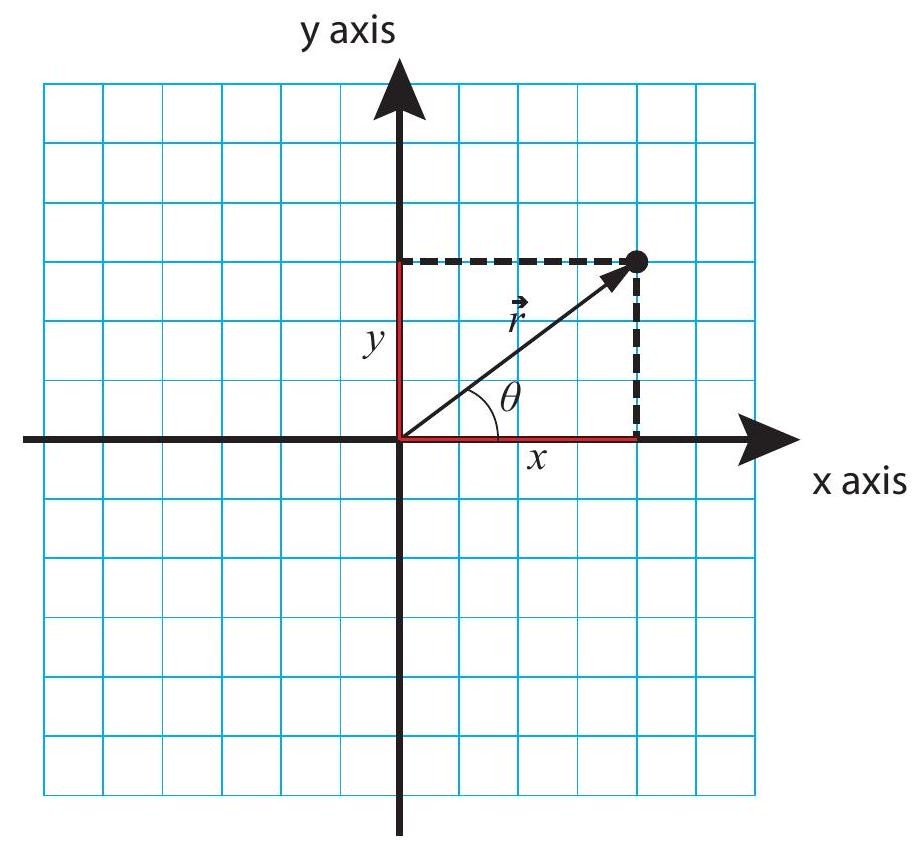
\includegraphics[max width=\textwidth]{2024_09_14_9969b06773f10b6936e8g-022}
\end{center}

Figure 1.1: The position vector, $\vec{r}$, of a point, and its $x$ and $y$ components (the point's coordinates).

The quantities $x$ and $y$ are taken to be positive or negative depending on what side of the origin the point is on. Typically, we will always start by choosing a positive direction for each axis, as the direction along which the algebraic value of the corresponding coordinate increases. This is often chosen to be to the right for the horizontal axis, and upwards for the vertical axis, but there is nothing that says we cannot choose a different convention if it turns out to be more convenient. In Figure 1.1, the arrows on the axes denote the positive direction for each. Going by the grid, the coordinates of the point shown are $x=4$ units, $y=3$ units.

In two or three dimensions (and even, in a sense, in one dimension), the coordinates of a point can\\
be interpreted as the components of a vector that we call the point's position vector, and denote by $\vec{r}$ (sometimes boldface letters are used for vectors, instead of an arrow on top; in that case, the position vector would be denoted by $\mathbf{r}$ ). A vector is a mathematical object, with specific geometric and algebraic properties, that physicists use to represent a quantity that has both a magnitude and a direction. The magnitude of the position vector in Fig. 1.1 is just the length of the arrow, which is to say, 5 length units (by the Pythagorean theorem, the length of $\vec{r}$, which we will often write using absolute value bars as $|\vec{r}|$, is equal to $\sqrt{x^{2}+y^{2}}$ ); this is just the straight-line distance of the point to the origin. The direction of $\vec{r}$, on the other hand, can be specified in a number of ways; a common convention is to give the value of the angle that it makes with the positive $x$ axis, which I have denoted in the figure as $\theta$ (in this case, you can verify that $\left.\theta=\tan ^{-1}(y / x)=36.9^{\circ}\right)$. In three dimensions, two angles would be needed to completely specify the direction of $\vec{r}$.

As you can see, giving the magnitude and direction of $\vec{r}$ is a way to locate the point that is completely equivalent to giving its coordinates $x$ and $y$. By the same token, the coordinates $x$ and $y$ are a way to specify the vector $\vec{r}$ that is completely equivalent to giving its magnitude and direction. As I stated above, we call $x$ and $y$ the components (or sometimes, to be more specific, the Cartesian components) of the vector $\vec{r}$. In a sense all the vectors that will be introduced later on this semester will derive their geometric and algebraic properties from the position vector $\vec{r}$, so once you know how to deal with one vector, you can deal with them all. The geometric properties (by which I mean, how to relate a vector's components to its magnitude and direction) I have just covered, and will come back to later on in this chapter, and again in Chapter 8; the algebraic properties (how to add vectors and multiply them by ordinary numbers, which are called scalars in this context) I will introduce along the way.

For the first few chapters this semester, we are going to be primarily concerned with motion in one dimension (that is to say, along a straight line, backwards or forwards), in which case all we need to locate a point is one number, its $x$ (or $y$, or $z$ ) coordinate; we do not then need to worry particularly about vector algebra. Alternatively, we can simply say that a vector in one dimension is essentially the same as its only component, which is just a positive or negative number (the magnitude of the number being the magnitude of the vector, and its sign indicating its direction), and has the algebraic properties that follow naturally from that.

The description of the motion that we are aiming for is to find a function of time, which we denote by $x(t)$, that gives us the point's position (that is to say, the value of $x$ ) for any value of the time parameter, $t$. (See Eq. (1.10), below, for an example.) Remember that $x$ stands for a number that can be positive or negative (depending on the side of the origin the point is on), and has dimensions of length, so when giving a numerical value for it you must always include the appropriate units (meters, centimeters, miles...). Similarly, $t$ stands for the time elapsed since some more or less arbitrary "origin of time," or time zero. Normally $t$ should always be positive, but in special cases it may make sense to consider negative times (think of how we count years: "AD" would correspond to "positive" and "BC" would correspond to negative - the difference being that there is actually no year zero!). Anyway, $t$ also is a number with dimensions, and must be reported with its appropriate\\
units: seconds, minutes, hours, etc.

\begin{center}
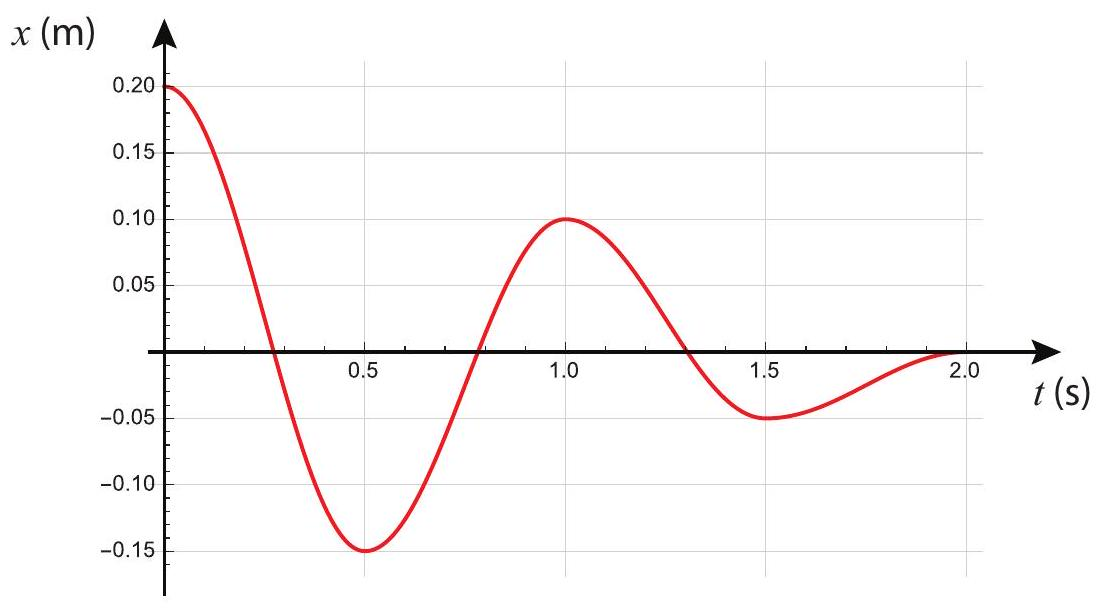
\includegraphics[max width=\textwidth]{2024_09_14_9969b06773f10b6936e8g-024}
\end{center}

Figure 1.2: A possible position vs. time graph for an object moving in one dimension.

We will be often interested in plotting the position of an object as a function of time - that is to say, the graph of the function $x(t)$. This may, in principle, have any shape, as you can see in Figure 1.2 above. In the lab, you will have a chance to use a position sensor that will automatically generate graphs like that for you on the computer, for any moving object that you aim the position sensor at. It is, therefore, important that you learn how to "read" such graphs. For example, Figure 1.2 shows an object that starts, at the time $t=0$, a distance 0.2 m away and to the right of the origin (so $x(0)=0.2 \mathrm{~m}$ ), then moves in the negative direction to $x=-0.15 \mathrm{~m}$, which it reaches at $t=0.5 \mathrm{~s}$; then turns back and moves in the opposite direction until it reaches the point $x=0.1 \mathrm{~m}$, turns again, and so on. Physically, this could be tracking the damped oscillations of a system such as an object attached to a spring and sliding over a surface that exerts a friction force on it (see Example 11.5.1).

\subsection*{1.2.2 Displacement}
In one dimension, the displacement of an object over a given time interval is a quantity that we denote as $\Delta x$, and equals the difference between the object's initial and final positions (in one dimension, we will often call the "position coordinate" simply the "position," for short):


\begin{equation*}
\Delta x=x_{f}-x_{i} \tag{1.1}
\end{equation*}


Here the subscript $i$ denotes the object's position at the beginning of the time interval considered, and the subscript $f$ its position at the end of the interval. The symbol $\Delta$ will consistently be used throughout this book to denote a change in the quantity following the symbol, meaning the\\
difference between its initial value and its final value. The time interval itself will be written as $\Delta t$ and can be expressed as


\begin{equation*}
\Delta t=t_{f}-t_{i} \tag{1.2}
\end{equation*}


where again $t_{i}$ and $t_{f}$ are the initial and final values of the time parameter (imagine, for instance, that you are reading time in seconds on a digital clock, and you are interested in the change in the object's position between second 130 and second 132: then $t_{i}=130 \mathrm{~s}, t_{2}=132 \mathrm{~s}$, and $\Delta t=2 \mathrm{~s}$ ).

You can practice reading off displacements from Figure 1.2. The displacement between $t_{i}=0.5 \mathrm{~s}$ and $t_{f}=1 \mathrm{~s}$, for instance, is $0.25 \mathrm{~m}\left(x_{i}=-0.15 \mathrm{~m}, x_{f}=0.1 \mathrm{~m}\right)$. On the other hand, between $t_{i}=1 \mathrm{~s}$ and $t_{f}=1.3 \mathrm{~s}$, the displacement is $\Delta x=0-0.1=-0.1 \mathrm{~m}$.

Notice two important things about the displacement. First, it can be positive or negative. Positive means the object moved, overall, in the positive direction; negative means it moved, overall, in the negative direction. Second, even when it is positive, the displacement does not always equal the distance traveled by the object (distance, of course, is always defined as a positive quantity), because if the object "doubles back" on its tracks for some distance, that distance does not count towards the overall displacement. For instance, looking again at Figure 1.2, in between the times $t_{i}=0.5 \mathrm{~s}$ and $t_{f}=1.5 \mathrm{~s}$ the object moved first 0.25 m in the positive direction, and then 0.15 m in the negative direction, for a total distance traveled of 0.4 m ; however, the total displacement was just 0.1 m .

In spite of these quirks, the total displacement is, mathematically, a useful quantity, because often we will have a way (that is to say, an equation) to calculate $\Delta x$ for a given interval, and then we can rewrite Eq. (1.1) so that it reads


\begin{equation*}
x_{f}=x_{i}+\Delta x \tag{1.3}
\end{equation*}


That is to say, if we know where the object started, and we have a way to calculate $\Delta x$, we can easily figure out where it ended up. You will see examples of this sort of calculation in the homework later on.

\section*{Extension to two dimensions}
In two dimensions, we write the displacement as the vector


\begin{equation*}
\Delta \vec{r}=\vec{r}_{f}-\vec{r}_{i} \tag{1.4}
\end{equation*}


The components of this vector are just the differences in the position coordinates of the two points involved; that is, $(\Delta \vec{r})_{x}$ (a subscript $x, y$, etc., is a standard way to represent the $x, y \ldots$ component of a vector) is equal to $x_{f}-x_{i}$, and similarly $(\Delta \vec{r})_{y}=y_{f}-y_{i}$.

\begin{center}
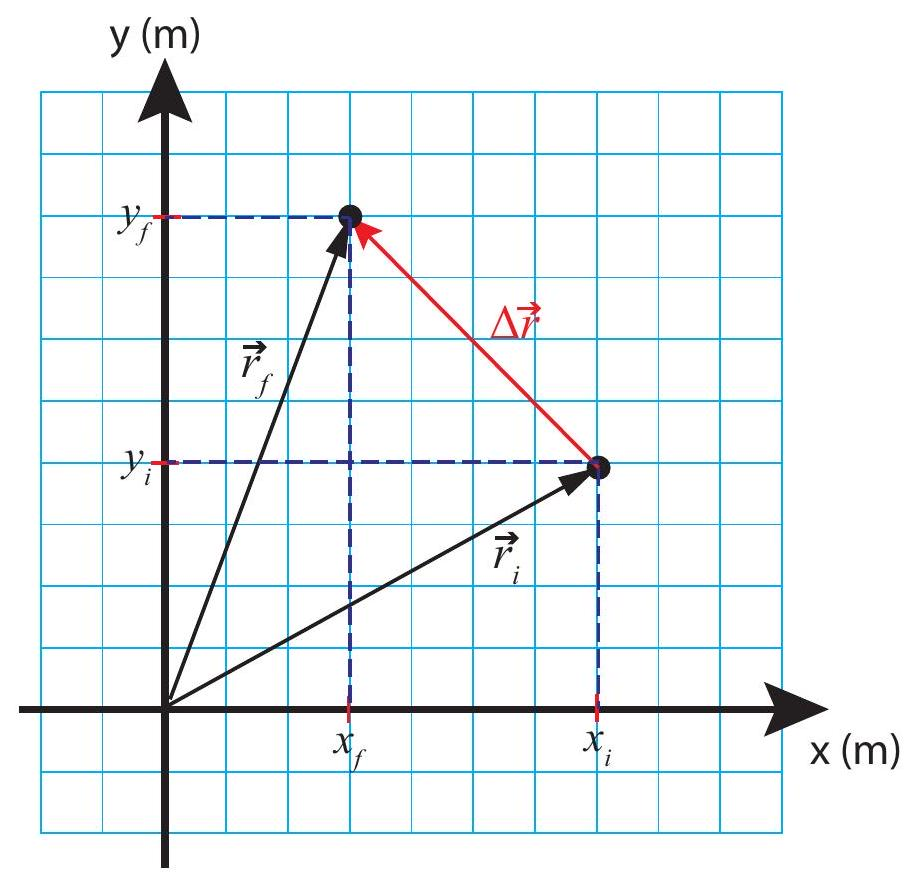
\includegraphics[max width=\textwidth]{2024_09_14_9969b06773f10b6936e8g-026}
\end{center}

Figure 1.3: The displacement vector for a particle that was initially at a point with position vector $\vec{r}_{i}$ and ended up at a point with position vector $\vec{r}_{f}$ is the difference of the position vectors.

Figure 1.3 shows how this makes sense. The $x$ component of $\Delta \vec{r}$ in the figure is $\Delta x=3-7=-4 \mathrm{~m}$; the $y$ component is $\Delta y=8-4=4 \mathrm{~m}$. This basically shows you how to subtract (and, by extension, add, since $\vec{r}_{f}=\vec{r}_{i}+\Delta \vec{r}$ ) vectors: you just subtract (or add) the corresponding components. Note how, by the Pythagorean theorem, the length (or magnitude) of the displacement vector, $|\Delta \vec{r}|=\sqrt{\left(x_{f}-x_{i}\right)^{2}+\left(y_{f}-y_{i}\right)^{2}}$, equals the straight-line distance between the initial point and the final point, just as in one dimension; of course, the particle could have actually followed a very different path from the initial to the final point, and therefore traveled a different distance.

\subsection*{1.2.3 Velocity}
\section*{Average velocity}
If you drive from Fayetteville to Fort Smith in 50 minutes, your average speed for the trip is calculated by dividing the distance of 59.2 mi by the time interval:


\begin{equation*}
\text { average speed }=\frac{\text { distance }}{\Delta t}=\frac{59.2 \mathrm{mi}}{50 \mathrm{~min}}=\frac{59.2 \mathrm{mi}}{50 \mathrm{~min}} \times \frac{60 \mathrm{~min}}{1 \mathrm{hr}}=71.0 \mathrm{mph} \tag{1.5}
\end{equation*}


(this equation, incidentally, also shows you how to convert units, and how you will be expected to\\
work with significant figures this semester: the rule of thumb is, keep four significant figures in all intermediate calculations, and report three in the final result).

The way we define average velocity is similar to average speed, but with one important difference: we use the displacement, instead of the distance. So, the average velocity $v_{a v}$ of an object, moving along a straight line, over a time interval $\Delta t$ is


\begin{equation*}
v_{a v}=\frac{\Delta x}{\Delta t} \tag{1.6}
\end{equation*}


This definition has all the advantages and the quirks of the displacement itself. On the one hand, it automatically comes with a sign (the same sign as the displacement, since $\Delta t$ will always be positive), which tells us in what direction we have been traveling. On the other hand, it may not be an accurate estimate of our average speed, if we doubled back at all. In the most extreme case, for a roundtrip (leave Fayetteville and return to Fayetteville), the average velocity would be zero, since $x_{f}=x_{i}$ and therefore $\Delta x=0$.

It is clear that this concept is not going to be very useful in general, if the object we are tracking has a chance to double back in the time interval $\Delta t$. A way to prevent this from happening, and also getting a more meaningful estimate of the object's speed at any instant, is to make the time interval very small. This leads to a new concept, that of instantaneous velocity.

\section*{Instantaneous velocity}
We define the instantaneous velocity of an object (a "particle"), at the time $t=t_{i}$, as the mathematical limit


\begin{equation*}
v=\lim _{\Delta t \rightarrow 0} \frac{\Delta x}{\Delta t} \tag{1.7}
\end{equation*}


The meaning of this is the following. Suppose we compute the ratio $\Delta x / \Delta t$ over successively smaller time intervals $\Delta t$ (all of them starting at the same time $t_{i}$ ). For instance, we can start by making $t_{f}=t_{i}+1 \mathrm{~s}$, then try $t_{f}=t_{i}+0.5 \mathrm{~s}$, then $t_{f}=t_{i}+0.1 \mathrm{~s}$, and so on. Naturally, as the time interval becomes smaller, the corresponding displacement will also become smaller-the particle has less and less time to move away from its initial position, $x_{i}$. The hope is that the successive ratios $\Delta x / \Delta t$ will converge to a definite value: that is to say, that at some point we will start getting very similar values, and that beyond a certain point making $\Delta t$ any smaller will not change any of the significant digits of the result that we care about. This limit value is the instantaneous velocity of the object at the time $t_{i}$.

When you think about it, there is something almost a bit self-contradictory about the concept of instantaneous velocity. You cannot (in practice) determine the velocity of an object if all you are given is a literal instant. You cannot even tell if the object is moving, if all you have is one instant! Motion requires more than one instant, the passage of time. In fact, all the "instantaneous" velocities that we can measure, with any instrument, are always really average velocities, only the\\
average is taken over very short time intervals. Nevertheless, the fact is that for any reasonably well-behaved position function $x(t)$, the limit in Eq. (1.7) is mathematically well-defined, and it equals what we call, in calculus, the derivative of the function $x(t)$ :


\begin{equation*}
v=\lim _{\Delta t \rightarrow 0} \frac{\Delta x}{\Delta t}=\frac{d x}{d t} \tag{1.8}
\end{equation*}


\begin{center}
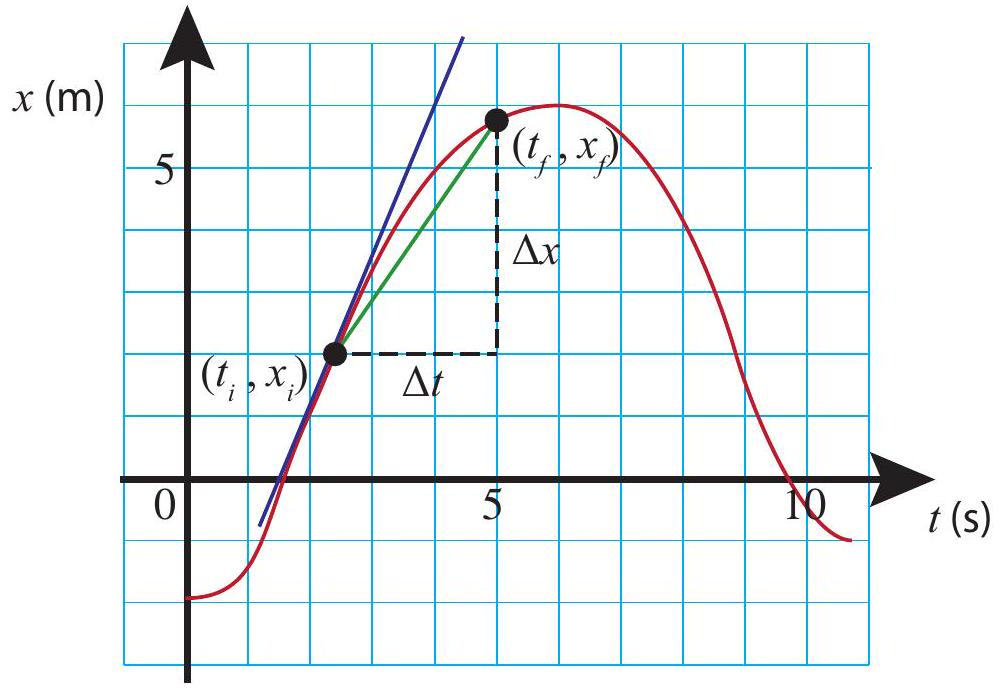
\includegraphics[max width=\textwidth]{2024_09_14_9969b06773f10b6936e8g-028}
\end{center}

Figure 1.4: The slope of the green segment is the average velocity for the time interval $\Delta t$ shown. As $\Delta t$ becomes smaller, this approaches the slope of the tangent at the point $\left(t_{i}, x_{i}\right)$

In fact, there is a nice geometric interpretation for this quantity: namely, it is the slope of a line tangent to the $x$-vs- $t$ curve at the point $\left(t_{i}, x_{i}\right)$. As Figure 1.4 shows, the average velocity $\Delta x / \Delta t$ is the slope (rise over run) of a line segment drawn from the point $\left(t_{i}, x_{i}\right)$ to the point $\left(t_{f}, x_{f}\right)$ (the green line in the figure). As we make the time interval smaller, by bringing $t_{f}$ closer to $t_{i}$ (and hence, also, $x_{f}$ closer to $x_{i}$ ), the slope of this segment will approach the slope of the tangent line at $\left(t_{i}, x_{i}\right)$ (the blue line), and this will be, by the definition (1.7), the instantaneous velocity at that point.

This geometric interpretation makes it easy to get a qualitative feeling, from the position-vs-time graph, for when the particle is moving more or less fast. A large slope means a steep rise or fall, and that is when the velocity will be largest - in magnitude. A steep rise means a large positive velocity, whereas a steep drop means a large negative velocity, by which I mean a velocity that is given by a negative number which is large in absolute value. In the future, to simplify sentences like this one, I will just use the word "speed" to refer to the magnitude (that is to say, the absolute value) of the instantaneous velocity. Thus, speed (like distance) is always a positive number, by definition, whereas velocity can be positive or negative; and a steep slope (positive or negative) means the speed is large there.

Conversely, looking at the sample $x$-vs- $t$ graphs in this chapter, you may notice that there are times when the tangent is horizontal, meaning it has zero slope, and so the instantaneous velocity at those times is zero (for instance, at the time $t=1.0 \mathrm{~s}$ in Figure 1.2). This makes sense when you think of what the particle is actually doing at those special times: it is just changing direction, so its velocity is going, for instance, from positive to negative. The way this happens is, it slows down, down... the velocity gets smaller and smaller, and then, for just an instant (literally, a mathematical point in time), it becomes zero before, the next instant, going negative.

We will be coming back to this "reading of graphs" in the lab and the homework, as well as in the next chapter, when we introduce the concept of acceleration.

\section*{Motion with constant velocity}
If the instantaneous velocity of an object never changes, it means that it is always moving in the same direction with the same speed. In that case, the instantaneous velocity and the average velocity coincide, and that means we can write $v=\Delta x / \Delta t$ (where the size of the interval $\Delta t$ could now be anything), and rewrite this equation in the form


\begin{equation*}
\Delta x=v \Delta t \tag{1.9}
\end{equation*}


which is the same as

$$
x_{f}-x_{i}=v\left(t_{f}-t_{i}\right)
$$

Now suppose we keep $t_{i}$ constant (that is, we fix the initial instant) but allow the time $t_{f}$ to change, so we will just write $t$ for an arbitrary value of $t_{f}$, and $x$ for the corresponding value of $x_{f}$. We end up with the equation

$$
x-x_{i}=v\left(t-t_{i}\right)
$$

which we can also write as


\begin{equation*}
x(t)=x_{i}+v\left(t-t_{i}\right) \tag{1.10}
\end{equation*}


after some rearranging, and where the notation $x(t)$ has been introduced to emphasize that we want to think of $x$ as a function of $t$. This is, not surprisingly, the equation of a straight line - a "curve" which is its own tangent and always has the same slope.\\
(Please make sure that you are not confused by the notation in Eq. (1.10). The parentheses around the $t$ on the left-hand side mean that we are considering the position $x$ as a function of $t$. On the other hand, the parentheses around the quantity $t-t_{i}$ on the right-hand side mean that we are multiplying this quantity by $v$, which is a constant here. This distinction will be particularly important when we introduce the function $v(t)$ next.)

Either one of equations (1.9) or (1.11) can be used to solve problems involving motion with constant velocity, and again you will see examples of this in the homework.

\section*{Motion with changing velocity}
If the velocity changes with time, obtaining an expression for the position of the object as a function of time may be a nontrivial task. In the next chapter we will study an important special case, namely, when the velocity changes at a constant rate (constant acceleration).

For the most general case, a graphical method that is sometimes useful is the following. Suppose that we know the function $v(t)$, and we graph it, as in Figure 1.5 below. Then the area under the curve in between any two instants, say $t_{i}$ and $t_{f}$, is equal to the total displacement of the object over that time interval.

The idea involved is known in calculus as integration, and it goes as follows. Suppose that I break

\begin{center}
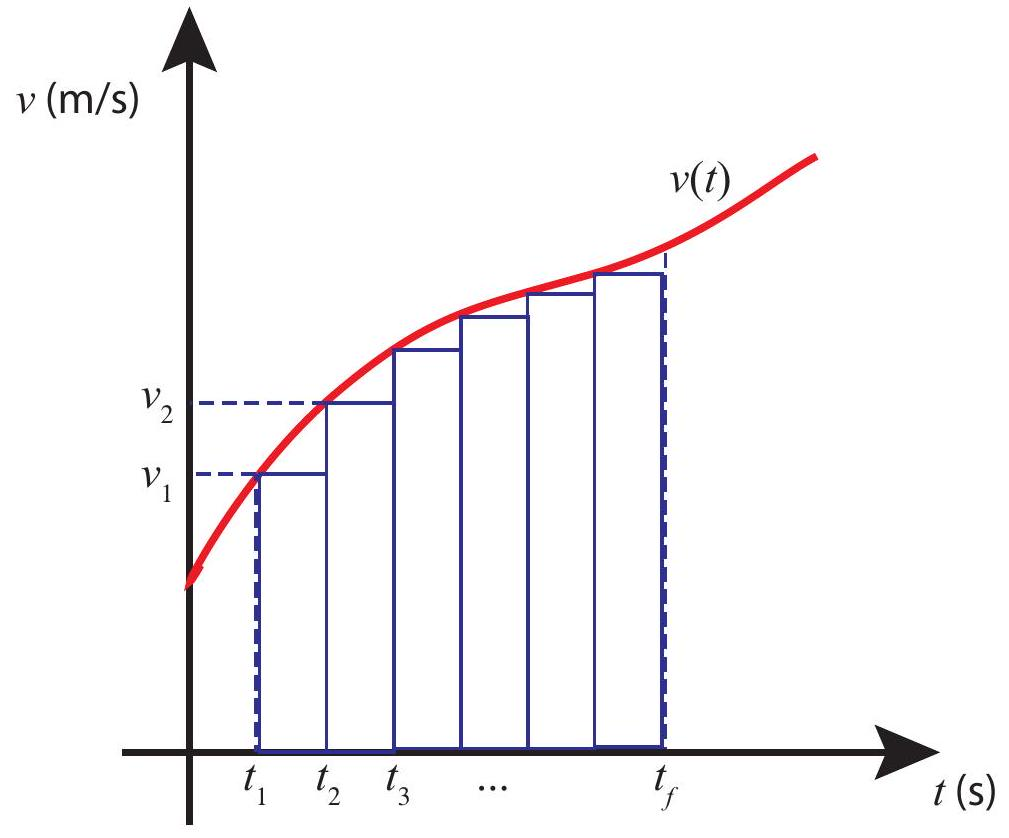
\includegraphics[max width=\textwidth]{2024_09_14_9969b06773f10b6936e8g-030}
\end{center}

Figure 1.5: How to get the displacement from the area under the $v$-vs- $t$ curve.\\
down the interval from $t_{i}$ to $t_{f}$ into equally spaced subintervals, beginning at the time $t_{i}$ (which I am, equivalently, going to call $t_{1}$, that is, $t_{1} \equiv t_{i}$, so I have now $t_{1}, t_{2}, t_{3}, \ldots t_{f}$ ). Now suppose I treat the object's motion over each subinterval as if it were motion with constant velocity, the velocity being that at the beginning of the subinterval. This, of course, is only an approximation, since the velocity is constantly changing; but, if you look at Figure 1.5, you can convince yourself that it will become a better and better approximation as I increase the number of intermediate points and the rectangles shown in the figure become narrower and narrower. In this approximation, the displacement during the first subinterval would be


\begin{equation*}
\Delta x_{1}=v_{1}\left(t_{2}-t_{1}\right) \tag{1.11}
\end{equation*}


where $v_{1}=v\left(t_{1}\right)$; similarly, $\Delta x_{2}=v_{2}\left(t_{3}-t_{2}\right)$, and so on.

However, Eq. (1.11) is just the area of the first rectangle shown under the curve in Figure 1.5 (the base of the rectangle has "length" $t_{2}-t_{1}$, and its height is $v_{1}$ ). Similarly for the second rectangle, and so on. So the sum $\Delta x_{1}+\Delta x_{2}+\ldots$ is both an approximation to the area under the $v$-vs-t curve, and an approximation to the total displacement $\Delta t$. As the subdivision becomes finer and finer, and the rectangles narrower and narrower (and more numerous), both approximations become more and more accurate. In the limit of "infinitely many," infinitely narrow rectangles, you get both the total displacement and the area under the curve exactly, and they are both equal to each other. Mathematically, we would write


\begin{equation*}
\Delta x=\int_{t_{i}}^{t_{f}} v(t) d t \tag{1.12}
\end{equation*}


where the stylized "S" (for "sum") on the right-hand side is the symbol of the operation known as integration in calculus. This is essentially the inverse of the process know as differentiation, by which we got the velocity function from the position function, back in Eq. (1.8).

This graphical method to obtain the displacement from the velocity function is sometimes useful, if you can estimate the area under the $v$-vs- $t$ graph reliably. An important point to keep in mind is that rectangles under the horizontal axis (corresponding to negative velocities) have to be added as having negative area (since the corresponding displacement is negative); see example 1.5.1 at the end of this chapter.

\section*{Extension to two dimensions}
In two (or more) dimensions, you define the average velocity vector as a vector $\vec{v}_{a v}$ whose components are $v_{a v, x}=\Delta x / \Delta t, v_{a v, y}=\Delta y / \Delta t$, and so on (where $\Delta x, \Delta y, \ldots$ are the corresponding components of the displacement vector $\Delta \vec{r})$. This can be written equivalently as the single vector equation


\begin{equation*}
\vec{v}_{a v}=\frac{\Delta \vec{r}}{\Delta t} \tag{1.13}
\end{equation*}


This tells you how to multiply (or divide) a vector by an ordinary number: you just multiply (or divide) each component by that number. Note that, if the number in question is positive, this operation does not change the direction of the vector at all, it just scales it up or down (which is why ordinary numbers, in this context, are called scalars). If the scalar is negative, the vector's direction is flipped as a result of the multiplication. Since $\Delta t$ in the definition of velocity is always positive, it follows that the average velocity vector always points in the same direction as the displacement, which makes sense.

To get the instantaneous velocity, you just take the limit of the expression (1.13) as $\Delta t \rightarrow 0$, for each component separately. The resulting vector $\vec{v}$ has components $v_{x}=\lim _{\Delta t \rightarrow 0} \Delta x / \Delta t$, etc., which can also be written as $v_{x}=d x / d t, v_{y}=d y / d t, \ldots$.

All the results derived above hold for each spatial dimension and its corresponding velocity component. For instance, the graphical method shown in Figure 1.5 can always be used to get $\Delta x$ if\\
the function $v_{x}(t)$ is known, or equivalently to get $\Delta y$ if you know $v_{y}(t)$, and so on.\\
Introducing the velocity vector at this point does cause a little bit of a notational difficulty. For quantities like $x$ and $\Delta x$, it is pretty obvious that they are the $x$ components of the vectors $\vec{r}$ and $\Delta \vec{r}$, respectively; however, the quantity that we have so far been calling simply $v$ should more properly be denoted as $v_{x}$ (or $v_{y}$ if the motion is along the $y$ axis). In fact, there is a convention that if you use the symbol for a vector without the arrow on top or any $x, y, \ldots$ subscripts, you must mean the magnitude of the vector. In this book, however, I have decided not to follow that convention, at least not until we get to Chapter 8 (and even then I will use it only for forces). This is because we will spend most of our time dealing with motion in only one dimension, and it makes the notation unnecessarily cumbersome to keep having to write the $x$ or $y$ subscripts on every component of every vector, when you really only have one dimension to worry about in the first place. So $v$ will, throughout, refer to the relevant component of the velocity vector, to be inferred from the context, until we get to Chapter 8 and actually need to deal with both a $v_{x}$ and a $v_{y}$ explicitly.

Finally, notice that the magnitude of the velocity vector, $|\vec{v}|=\sqrt{v_{x}^{2}+v_{y}^{2}+v_{z}^{2}}$, is equal to the instantaneous speed, since, as $\Delta t \rightarrow 0$, the magnitude of the displacement vector, $|\Delta \vec{r}|$, becomes the actual distance traveled by the object in the time interval $\Delta t$.

\subsection*{1.3 Reference frame changes and relative motion}
Everything up to this point assumes that we are using a fixed, previously agreed upon reference frame. Basically, this is just an origin and a set of axes along which to measure our coordinates, as shown in Figure 1.

There are, however, a number of situations in physics that call for the use of different reference frames, and, more importantly, that require us to convert various physical quantities from one reference frame to another. For instance, imagine you are on a boat on a river, rowing downstream. You are moving with a certain velocity relative to the water around you, but the water itself is flowing with a different velocity relative to the shore, and your actual velocity relative to the shore is the sum of those two quantities. Ships generally have to do this kind of calculation all the time, as do airplanes: the "airspeed" is the speed of a plane relative to the air around it, but that air is usually moving at a substantial speed relative to the earth.

The way we deal with all these situations is by introducing two reference frames, which here I am going to call A and B. One of them, say A, is "at rest" relative to the earth, and the other one is "at rest" relative to something else-which means, really, moving along with that something else. (For instance, a reference frame at rest "relative to the river" would be a frame that's moving along\\
with the river water, like a piece of driftwood that you could measure your progress relative to.)\\
In any case, graphically, this will look as in Figure 1.6, which I have drawn for the two-dimensional case because I think it makes it easier to visualize what's going on:

\begin{center}
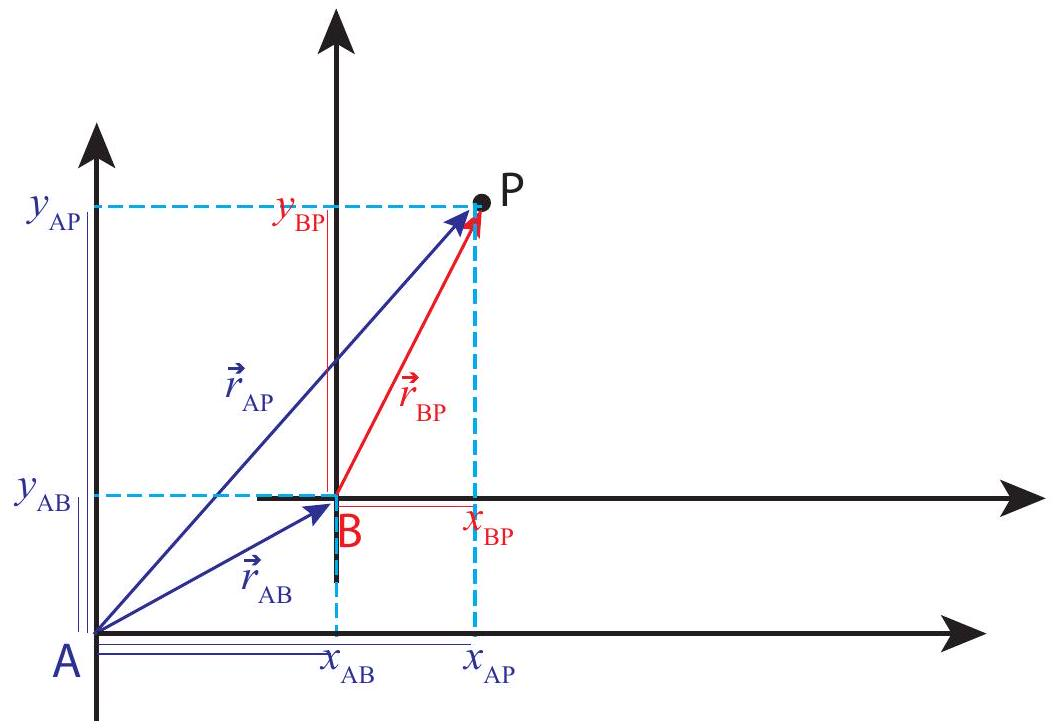
\includegraphics[max width=\textwidth]{2024_09_14_9969b06773f10b6936e8g-033}
\end{center}

Figure 1.6: Position vectors and coordinates of a point $P$ in two different reference frames, A and B .

In the reference frame A, the point $P$ has position coordinates $\left(x_{A P}, y_{A P}\right)$. Likewise, in the reference frame B, its coordinates are $\left(x_{B P}, y_{B P}\right)$. As you can see, the notation chosen is such that every coordinate in A will have an "A" as a first subscript, while the second subscript indicates the object to which it refers, and similarly for coordinates in B.

The coordinates $\left(x_{A B}, y_{A B}\right)$ are special: they are the coordinates, in the reference frame A , of the origin of reference frame B. This is enough to fully locate the frame B in A, as long as the frames are not rotated relative to each other.

The thin colored lines I have drawn along the axes in Figure 1.6 are intended to make it clear that the following equations hold:


\begin{align*}
x_{A P} & =x_{A B}+x_{B P} \\
y_{A P} & =y_{A B}+y_{B P} \tag{1.14}
\end{align*}


Although the figure is drawn for the easy case where all these quantities are positive, you should be able to convince yourself that Eqs. (1.14) hold also when one or more of the coordinates have negative values.

All these coordinates are also the components of the respective position vectors, shown in the figure and color-coded by reference frame (so, for instance, $\vec{r}_{A P}$ is the position vector of $P$ in the frame A), so the equations (1.14) can be written more compactly as the single vector equation


\begin{equation*}
\vec{r}_{A P}=\vec{r}_{A B}+\vec{r}_{B P} \tag{1.15}
\end{equation*}


From all this you can see how to add vectors: algebraically, you just add their components separately, as in Eqs. (1.14); graphically, you draw them so the tip of one vector coincides with the tail of the other (we call this "tip-to-tail"), and then draw the sum vector from the tail of the first one to the tip of the other one. (In general, to get two arbitrary vectors tip-to-tail you may need to displace one of them; this is OK provided you do not change its orientation, that is, provided you only displace it, not rotate it. We'll see how this works in a moment with velocities, and later on with forces.)

Of course, I showed you already how to subtract vectors with Fig. 1.3: again, algebraically, you just subtract the corresponding coordinates, whereas graphically you draw them with a common origin, and then draw the vector from the tip of the vector you are subtracting to the tip of the other one. If you read the previous paragraph again, you can see that Fig. 1.3 can equally well be used to show that $\Delta \vec{r}=\vec{r}_{f}-\vec{r}_{i}$, as to show that $\vec{r}_{f}=\vec{r}_{i}+\Delta \vec{r}$.

In a similar way, you can see graphically from Fig. 1.6 (or algebraically from Eq. (1.15)) that the position vector of $P$ in the frame B is given by $\vec{r}_{B P}=\vec{r}_{A P}-\vec{r}_{A B}$. The last term in this expression can be written in a different way, as follows. If I follow the convention I have introduced above, the quantity $x_{B A}$ (with the order of the subscripts reversed) would be the $x$ coordinate of the origin of frame A in frame B, and algebraically that would be equal to $-x_{A B}$, and similarly $y_{B A}=-y_{A B}$. Hence the vector equality $\vec{r}_{A B}=-\vec{r}_{B A}$ holds. Then,


\begin{equation*}
\vec{r}_{B P}=\vec{r}_{A P}-\vec{r}_{A B}=\vec{r}_{A P}+\vec{r}_{B A} \tag{1.16}
\end{equation*}


This is, in a way, the "inverse" of Eq. (1.15): it tells us how to get the position of $P$ in the frame B if we know its position in the frame A.

Let me show next you how all this extends to displacements and velocities. Suppose the point $P$ indicates the position of a particle at the time $t$. Over a time interval $\Delta t$, both the position of the particle and the relative position of the two reference frames may change. We can add yet another subscript, $i$ or $f$, (for initial and final) to the coordinates, and write, for example,


\begin{align*}
x_{A P, i} & =x_{A B, i}+x_{B P, i} \\
x_{A P, f} & =x_{A B, f}+x_{B P, f} \tag{1.17}
\end{align*}


Subtracting these equations gives us the corresponding displacements:


\begin{equation*}
\Delta x_{A P}=\Delta x_{A B}+\Delta x_{B P} \tag{1.18}
\end{equation*}


Dividing Eq. (1.18) by $\Delta t$ we get the average velocities ${ }^{1}$, and then taking the limit $\Delta t \rightarrow 0$ we get the instantaneous velocities. This applies in the same way to the $y$ coordinates, and the result is the vector equation


\begin{equation*}
\vec{v}_{A P}=\vec{v}_{B P}+\vec{v}_{A B} \tag{1.19}
\end{equation*}


I have rearranged the terms on the right-hand side to (hopefully) make it easier to visualize what's going on. In words: the velocity of the particle $P$ relative to (or measured in) frame A is equal to the (vector) sum of the velocity of the particle as measured in frame B, plus the velocity of frame B relative to frame A.

The result (1.19) is just what we would have expected from the examples I mentioned at the beginning of this section, like rowing in a river or an airplane flying in the wind. For instance, for the airplane $\vec{v}_{B P}$ could be its "airspeed" (only it has to be a vector, so it would be more like its "airvelocity": that is, its velocity relative to the air around it), and $\vec{v}_{A B}$ would be the velocity of the air relative to the earth (the wind velocity, at the location of the airplane). In other words, A represents the earth frame of reference and B the air, or wind, frame of reference. Then, $\vec{v}_{A P}$ would be the "true" velocity of the airplane relative to the earth. You can see how it would be important to add these quantities as vectors, in general, by considering what happens when you fly in a cross wind, or try to row across a river, as in Figure 1.7 below.

\begin{center}
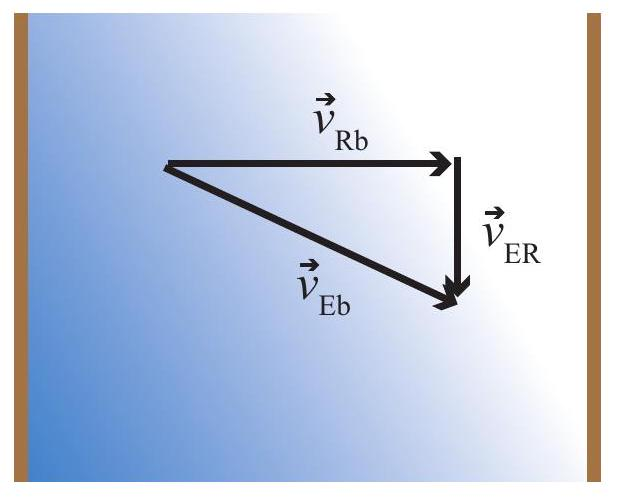
\includegraphics[max width=\textwidth]{2024_09_14_9969b06773f10b6936e8g-035}
\end{center}

Figure 1.7: Rowing across a river. If you head "straight across" the river (with velocity vector $\vec{v}_{R b}$ in the moving frame of the river, which is flowing with velocity $\vec{v}_{E R}$ in the frame of the earth), your actual velocity relative to the shore will be the vector $\vec{v}_{E b}$. This is an instance of Eq. (1.19), with frame A being E (the earth), frame B being R (the river), and "b" (for "boat") standing for the point P we are tracking.

As you can see from this couple of examples, Equation (1.19) is often useful as it is written, but

\footnotetext{${ }^{1}$ We have made a very natural assumption, that the time interval $\Delta t$ is the same for observers tracking the particle's motion in frames A and B, respectively (where each observer is understood to be moving along with his or her frame). This, however, turns out to be not true when any of the velocities involved is close to the speed of light, and so the simple addition of velocities formula (1.19) does not hold in Einstein's relativity theory.\\
(This is actually the first bit of real physics I have told you about in this book, so far; unfortunately, you will have no use for it this semester!)
}
sometimes the information we have is given to us in a different way: for instance, we could be given the velocity of the object in frame A $\left(\vec{v}_{A P}\right)$, and the velocity of frame B as seen in frame $\mathrm{A}\left(\vec{v}_{A B}\right)$, and told to calculate the velocity of the object as seen in frame B. This can be easily accomplished if we note that the vector $\vec{v}_{A B}$ is equal to $-\vec{v}_{B A}$; that is to say, the velocity of frame B as seen from frame A is just the opposite of the velocity of frame A as seen from frame B. Hence, Eq. (1.19) can be rewritten as\\
\$\$

\begin{equation*}
\vec{v}_{A P}=\vec{v}_{B P}-\vec{v}_{B A} \tag{1.20}
\end{equation*}

\$\$

For most of the next few chapters we are going to be considering only motion in one dimension, and so we will write Eq. (1.19) (or (1.20)) without the vector symbols, and it will be understood that $v$ refers to the component of the vector $\vec{v}$ along the coordinate axis of interest.

A quantity that will be particularly important later on is the relative velocity of two objects, which we could label 1 and 2 . The velocity of object 2 relative to object 1 is, by definition, the velocity which an observer moving along with 1 would measure for object 2 . So it is just a simple frame change: let the earth frame be frame E and the frame moving with object 1 be frame 1 , then the velocity we want is $v_{12}$ ("velocity of object 2 in frame 1 "). If we make the change $\mathrm{A} \rightarrow 1, \mathrm{~B} \rightarrow E$, and $\mathrm{P} \rightarrow 2$ in Eq. (1.20), we get


\begin{equation*}
v_{12}=v_{E 2}-v_{E 1} \tag{1.21}
\end{equation*}


In other words, the velocity of 2 relative to 1 is just the velocity of 2 minus the velocity of 1 . This is again a familiar effect: if you are driving down the highway at 50 miles per hour, and the car in front of you is driving at 55 , then its velocity relative to you is 5 mph , which is the rate at which it is moving away from you (in the forward direction, assumed to be the positive one).

It is important to realize that all these velocities are real velocities, each in its own reference frame. Something may be said to be truly moving at some velocity in one reference frame, and just as truly moving with a different velocity in a different reference frame. I will have a lot more to say about this in the next chapter, but in the meantime you can reflect on the fact that, if a car moving at 55 mph collides with another one moving at 50 mph in the same direction, the damage will be basically the same as if the first car had been moving at 5 mph and the second one had been at rest. For practical purposes, where you are concerned, another car's velocity relative to yours is that car's "real" velocity.

\section*{Resources}
A good app for practicing how to add vectors (and how to break them up into components, magnitude and direction, etc.) may be found here:\\
\href{https://phet.colorado.edu/en/simulation/vector-addition}{https://phet.colorado.edu/en/simulation/vector-addition}.\\
Perhaps the most dramatic demonstration of how Eq. (1.19) works in the real world is in this episode of Mythbusters: \href{https://www.youtube.com/watch?v=BLuI118nhzc}{https://www.youtube.com/watch?v=BLuI118nhzc}. (If this link does not work, do a search for "Mythbusters cancel momentum.") They shoot a ball from the bed of a truck,\\
with a velocity (relative to the truck) of 60 mph backwards, while the truck is moving forward at 60 mph. I think the result is worth watching. (Do not be distracted by their talk about momentum. We will get there, in time.)

A very old, but also very good, educational video about different frames of reference is this one: \href{https://www.youtube.com/watch?v=sS17fComONs}{https://www.youtube.com/watch?v=sS17fComONs}. You should try to watch at least part of it. Many things will be relevant to later parts of the course, including projectile motion, and the whole discussion of relative motion coming up next, in Chapter 2.

\subsection*{1.4 In summary}
\begin{enumerate}
  \item To describe the motion of an object in one dimension we treat it as a mathematical point, and consider its position coordinate, $x$ (often shortened to just the position), as a function of time: $x(t)$.
  \item Numerically, the position coordinate is the distance to a chosen origin, with a positive or negative sign depending on which side of the origin the point is. For every problem, when we introduce a coordinate axis we need to specify a positive direction. Starting from the origin in that direction, the position coordinate is positive and increasing, whereas going from the origin in the opposite direction (negative direction) it becomes increasingly negative.
  \item The displacement of an object over a time interval from an initial time $t_{i}$ to a final time $t_{f}$ is the quantity $\Delta x=x_{f}-x_{i}$, where $x_{f}$ is the position of the object at the final time (or, the final position), and $x_{i}$ the position at the initial time (or initial position).
  \item The average velocity of an object over the time interval from $t_{i}$ to $t_{f}$ is defined as $v_{a v}=\Delta x / \Delta t$, where $\Delta t=t_{f}-t_{i}$.
  \item The instantaneous velocity (often just called the velocity) of an object at the time $t$ is the limit value of the quantity $\Delta x / \Delta t$, calculated for successively shorter time intervals $\Delta t$, all with the same initial time $t_{i}=t$. This is, mathematically, the definition of the derivative of the function $x(t)$ at the time $t$, which we express as $v=d x / d t$.
  \item Graphically, the instantaneous velocity of the object at the time $t$ is the slope of the tangent line to the $x$-vs-t graph at the time $t$.
  \item The instantaneous velocity of an object is a positive or negative quantity depending on whether the object, at that instant, is moving in the positive or the negative direction.
  \item For an object moving with constant velocity $v$, the position function is given by [Eq. (1.10)]:
\end{enumerate}

$$
x(t)=x_{i}+v\left(t-t_{i}\right)
$$

where $t_{i}$ is an arbitrarily chosen initial time and $x_{i}$ the position at that time. This can also be written in the form given by Eq. (1.9). The argument $(t)$ on the left-hand side of (1.10) is optional, and $t_{i}$ is often set equal to zero, giving just $x=x_{i}+v t$. This, however, is not quite as generally applicable as the result (1.9) or (1.10).\\
9. For an object moving with changing velocity, the total displacement in between times $t_{i}$ and $t_{f}$ is equal to the total area under the $v$-vs- $t$ curve in between those times; areas below the horizontal $(t)$ axis must be treated as negative.\\
10. In two or more dimensions one introduces, for every point in space, a position vector whose components are just the Cartesian coordinates of that point; then the displacement vector is defined as $\Delta \vec{r}=\vec{r}_{f}-\vec{r}_{i}$, the average velocity vector is $\vec{v}_{a v}=\Delta \vec{r} / \Delta t$, and the instantaneous velocity vector is the limit of this as $\Delta t$ goes to zero. Vectors are added by adding their components separately; to multiply a vector by an ordinary number, or scalar, we just multiply each component by that number.\\
11. When tracking the motion of an object, "P", in two different reference frames, A and B , the position vectors are related by $\vec{r}_{A P}=\vec{r}_{A B}+\vec{r}_{B P}$, and likewise the velocity vectors: $\vec{v}_{A P}=\vec{v}_{A B}+\vec{v}_{B P}$. Here, the first subscript tells you in which reference frame you are measuring, and the second subscript what it is that you are looking at; $\vec{r}_{A B}$ is the position vector of the origin of frame B as seen in frame A , and $\vec{v}_{A B}$ its velocity.

\subsection*{1.5 Examples}
\subsection*{1.5.1 Motion with (piecewise) constant velocity}
You leave your house on your bicycle to go visit a friend. At your normal speed of 9 mph , you know it takes you 6 minutes to get there. This time, though, when you have traveled half the distance you realize you forgot a book at home that you were going to return to your friend, so you turn around and pedal at twice your normal speed, get back home, grab the book, and start off again for your friend's house at 18 mph (imagine you are really fit to pull this off!)\\
(a) How far away from you does your friend live?\\
(b) What is the total distance you travel on this trip?\\
(c) How long did the whole trip take?\\
(d) Draw a position versus time and a velocity versus time graph for the whole trip. Use SI units for both graphs. Neglect the time it takes you to stop and turn around, and also the time it takes you to run into your house and grab the book (in other words, assume those changes in your direction of motion happen instantly).\\
(e) Show explicitly, using your $v$-vs- $t$ graph, that the graphical method of Figure 1.5 gives you the total displacement for your trip.

\section*{Solution}
I am going to work out this problem using both miles and SI units, the first because it seems most natural, and the second because we are asked to use SI units for part (d), so we might as well use them from the start. In general, you should use SI units whenever you can. If you are unsure of what to do in a specific problem, ask your instructor!\\
(a) We are told that at 9 miles per hour it would take 6 minutes to get there, so let us use


\begin{equation*}
\Delta x=v \Delta t \tag{1.22}
\end{equation*}


with $v=9 \mathrm{mph}$ and $\Delta t=6 \mathrm{~min}$. We have to either convert the hours to minutes, or vice-versa. Again, in this case it seems easiest to realize that 6 min equals $1 / 10$ of an hour, so:


\begin{equation*}
\Delta x=\left(9 \frac{\text { miles }}{\mathrm{hr}}\right) \times 0.1 \mathrm{hr}=0.9 \text { miles } \tag{1.23}
\end{equation*}


In SI units, $9 \mathrm{mph}=4.023 \mathrm{~m} / \mathrm{s}$, and $6 \mathrm{~min}=360 \mathrm{~s}$, so $\Delta x=1448 \mathrm{~m}$.\\
(b) This is just a matter of keeping track of the distance traveled in the various parts of the trip. You start by riding half the distance to your friend's house, which is to say, 0.45 miles, and then you ride that again back home, so that's 0.9 miles, and then you're back where you started, so you still have to go the 0.9 miles to your friend's house. So overall, you ride for 1.8 miles, or 2897 m .\\
(c) The whole trip consists, as detailed above, of 0.45 miles at 9 mph , and the rest, which is 1.35 miles, at 18 mph . Applying $\Delta t=\Delta x / v$ to each of these intervals, we get a total time of


\begin{align*}
\Delta t & =\frac{0.45 \mathrm{miles}}{9 \mathrm{mph}}+\frac{1.35 \mathrm{miles}}{18 \mathrm{mph}}=0.125 \text { hours } \\
& =0.125 \times 60 \mathrm{~min}=7.5 \mathrm{~min} \\
& =7.5 \times 60 \mathrm{~s}=450 \mathrm{~s} \tag{1.24}
\end{align*}


(d) The graphs are shown below. Details on how to get them follow.

\begin{center}
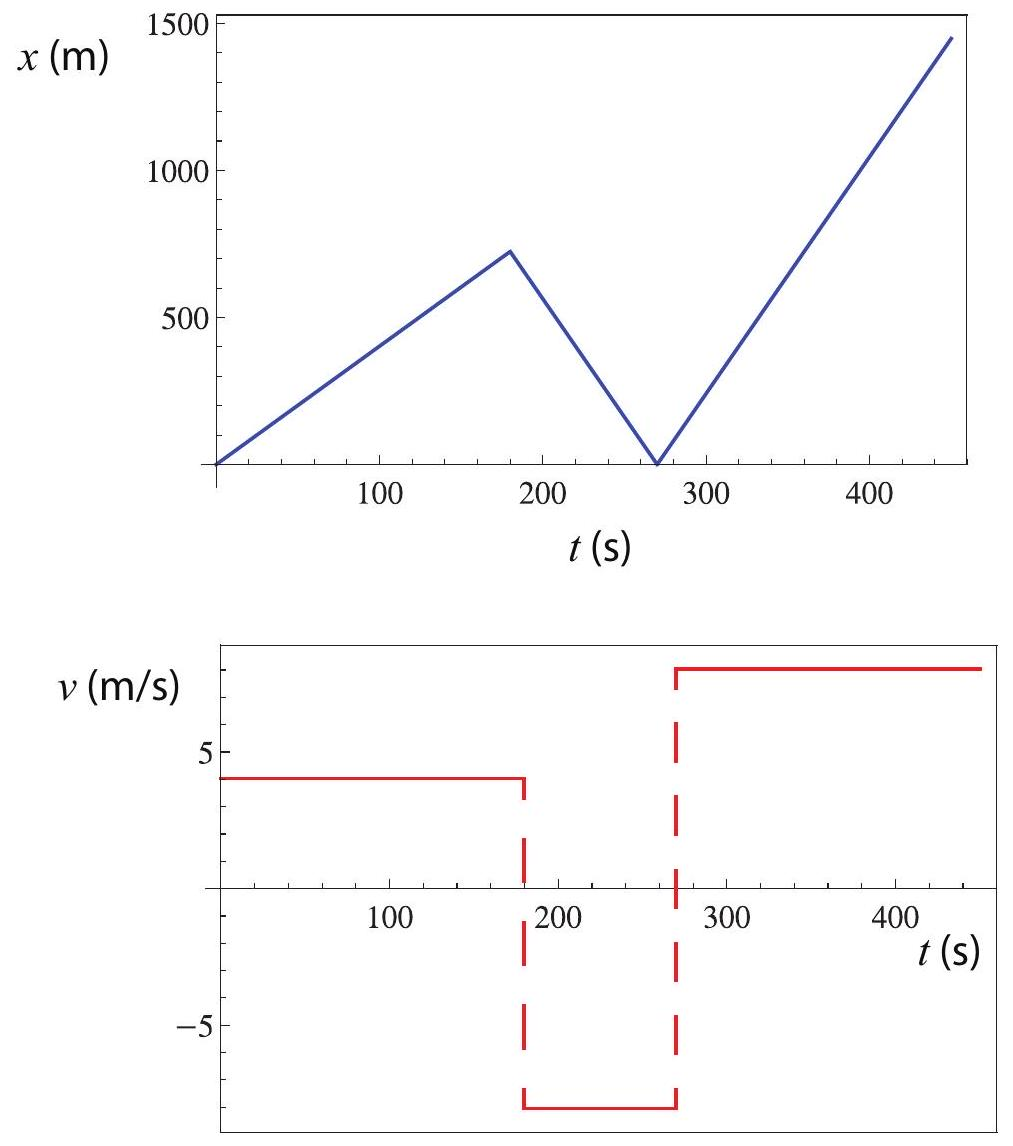
\includegraphics[max width=\textwidth]{2024_09_14_9969b06773f10b6936e8g-040}
\end{center}

\begin{itemize}
  \item First interval: from $t=0$ to $t=180 \mathrm{~s}$ ( 3 min , which is what it would take to cover half the distance to your friend's house at 9 mph ). The velocity is a constant $v=4.023 \mathrm{~m} / \mathrm{s}$. For the position graph, use Eq. (1.10) with $x_{i}=0, t_{i}=0$ and $v=4.023 \mathrm{~m} / \mathrm{s}$.
  \item Second interval: from $t=180 \mathrm{~s}$ to $t=270 \mathrm{~s}$ (it takes you half of 3 min , which is to say 90 s , to cover the same distance as above at twice the speed). The velocity is a constant $v=-8.046 \mathrm{~m} / \mathrm{s}$\\
(twice what it was earlier, but in the opposite direction). For the position graph, use Eq. (1.10) with $x_{i}=724 \mathrm{~m}$ (this is half of the distance to your friend's house, and the starting position for this interval), $t_{i}=180 \mathrm{~s}$ and $v=-8.046 \mathrm{~m} / \mathrm{s}$.
  \item Third interval: from $t=270 \mathrm{~s}$ to $t=450 \mathrm{~s}$. The velocity is a constant $v=8.046 \mathrm{~m} / \mathrm{s}$ (same speed as just before, but in the opposite direction). For the position graph, use Eq. (1.10) with $x_{i}=0 \mathrm{~m}$ (you start back at your house), $t_{i}=270 \mathrm{~s}$ and $v=8.046 \mathrm{~m} / \mathrm{s}$.
\end{itemize}

If you are familiar with the software package Mathematica, the position graph was produced using the command\\
$\operatorname{Plot}\left[\mathrm{If}\left[\mathrm{t}<180,4.023 \mathrm{t}, \mathrm{If}\left[\mathrm{t}<270,4.023^{*} 180-8.046(\mathrm{t}-180), 8.046(\mathrm{t}-270)\right]\right],\{\mathrm{t}, 0,450\}\right]$\\
and the velocity graph was produced using\\
Plot[If[t<180, 4.023, If $[\mathrm{t}<270,-8.046,8.046]],\{\mathrm{t}, 0,450\}]$\\
(and then connecting the horizontal lines by hand, which is not necessary, but helps to visualize what's going on).

The graphs could also have been produced using the free plotting software package Gnuplot (available here: \href{http://www.gnuplot.info/download.html}{http://www.gnuplot.info/download.html}) with the following commands: gnuplot $>$ set dummy $t$\\
gnuplot $>\mathrm{f}(\mathrm{t})=\mathrm{t}<180 ? 4.023^{*} \mathrm{t}: \mathrm{t}<270 ? 4.023^{*} 180-8.046^{*}(\mathrm{t}-180): 8.046^{*}(\mathrm{t}-270)$\\
gnuplot> plot $[0: 450] \mathrm{f}(\mathrm{t})$\\
The first line sets the default independent variable to $t$ (instead of $x$, which is what Gnuplot expects). The second line defines the piecewise function using the ternary operator (? :) borrowed from the C programming language. The third line plots the function over the range indicated.\\
(e) For this we need to find the area under the $v$-vs- $t$ graph we just plotted. Basically, we have three rectangles: the first one has base 180 units ( s ) and height 4 units ( $\mathrm{m} / \mathrm{s}$ ), so its area is $4 \times 180=720$ (m). The second rectangle has base 90 units and height -8 (negative, because it is below the horizontal axis!), so its area is -720 . The last one has base 180 units again (from 270 to 450 ) and height 8 , so its area is $8 \times 180=1440$. So the total area "under" the $v$-vs- $t$ curve is

$$
720-720+1440=1440 \text { meters }
$$

which is (approximately) your total displacement, that is, the 9 miles to your friend's house. (Of course, we would have obtained a more accurate result if we had used the more accurate values for the "heights" of $4.023,-8.046$, and 8.046 , but if all we have to go by is the graph, such accuracy is pretty much impossible.)

\subsection*{1.5.2 Addition of velocities, relative motion}
This example was inspired by the "race on a moving sidewalk" demo at \href{http://physics.bu.edu/}{http://physics.bu.edu/} duffy/classroom.html.\\
Please go take a look at it!\\
Two girls, Ann and Becky (yes, A and B) decide to have a race while they wait for a plane at a nearly-deserted airport. Ann will run on the moving walkway, to the end of it (which is 30 m away) and back, whereas Becky will run alongside her on the (non-moving) floor, also 30 m out and back. The walkway moves at $1 \mathrm{~m} / \mathrm{s}$, and the girls both run at the same constant speed of $5 \mathrm{~m} / \mathrm{s}$ relative to the surface they are standing on.\\
(a) Relative to the (non-moving) floor, what is Ann's velocity for the first leg of her race, when she is moving in the same direction as the walkway (take that to be the positive direction)? What is her velocity for the return leg?\\
(b) How long does it take each of the girls to complete their race?\\
(c) When both girls are running in the positive direction, what is Becky's velocity relative to Ann? (That is, how fast does Ann see Becky move, and in what direction?)\\
(d) When Ann turns around and starts running in the negative direction, but Becky is still running in the positive direction, what is Becky's velocity relative to Ann?\\
(e) What is the total distance Ann runs in the moving walkway's frame of reference?

\section*{Solution}
I am going to solve this in the format that you will be required to use this semester for most of the homework and exam problems. I will not be able to do this for every single example, but you should! Please follow this carefully.

To begin with, you must draw a sketch of the situation described in the problem, detailed enough to include all the relevant information you are given. Here is mine:\\
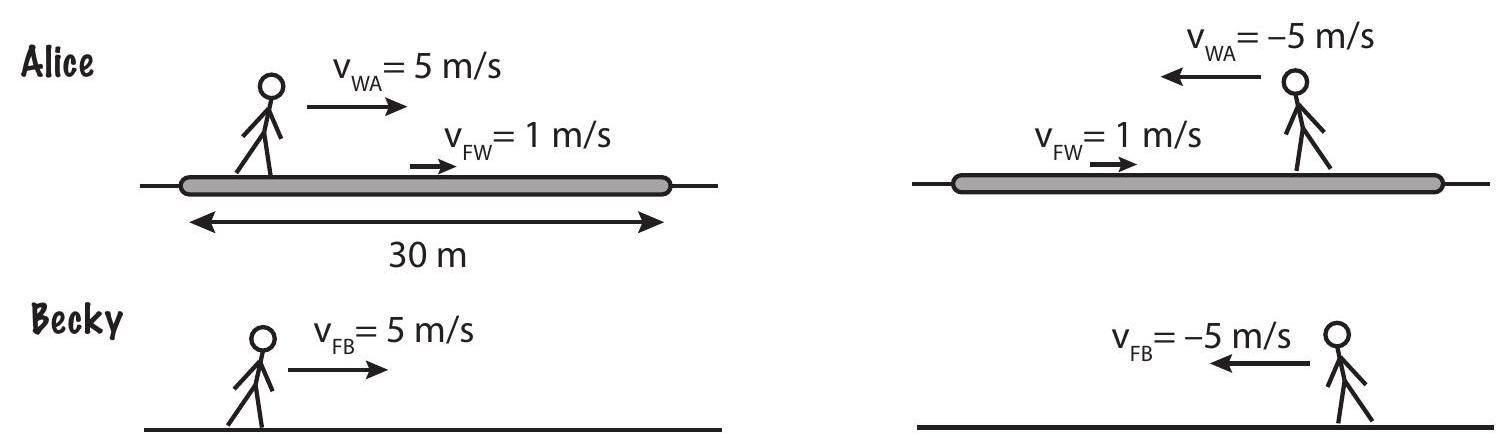
\includegraphics[max width=\textwidth, center]{2024_09_14_9969b06773f10b6936e8g-042(1)}\\
going out

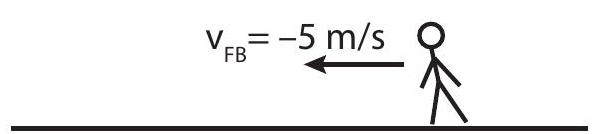
\includegraphics[max width=\textwidth, center]{2024_09_14_9969b06773f10b6936e8g-042}\\
coming back

Note that I have drawn one picture for each half of the race, and that all the information given in the text of the problem is there. The figure makes it clear also the notation I will be using for each of the girls' velocities, and to see at a glance what is happening.

You should next state what kind of problem this is and what basic result (theorem, principle, or equation(s)) you are going to use to solve it. For this problem, you could say:\\
"This is a relative motion/reference frame transformation problem. I will use Eq. (1.19)

$$
\vec{v}_{A P}=\vec{v}_{B P}+\vec{v}_{A B}
$$

as well as the basic equation for motion with constant velocity:"

$$
\Delta x=v \Delta t
$$

After that, solve each part in turn, and make sure to show all your work!\\
Part (a): Let $F$ stand for the floor frame of reference, and $W$ the walkway frame. In the notation of Section 1.3, we have $v_{F W}=1 \mathrm{~m} / \mathrm{s}$. For the first leg of her race, we are told that Ann's velocity relative to the walkway is $5 \mathrm{~m} / \mathrm{s}$, so $v_{W A}=5 \mathrm{~m} / \mathrm{s}$. Then, by Eq. (1.19) (with the following change of indices: $A \rightarrow F, B \rightarrow W$, and $P \rightarrow A$,


\begin{equation*}
v_{F A}=v_{F W}+v_{W A}=1 \frac{\mathrm{m}}{\mathrm{s}}+5 \frac{\mathrm{m}}{\mathrm{s}}=6 \frac{\mathrm{m}}{\mathrm{s}} \tag{1.25}
\end{equation*}


(when you see an equation like this, full of subscripts, it is a good practice to read it out, mentally, to yourself: "Ann's velocity relative to the floor equals the velocity of the walkway relative to the floor plus Ann's velocity relative to the walkway." Then take a moment to see if it makes sense! Here is a place where the picture can be really helpful.)

For the return leg, use the same formula, but note that now her velocity relative to the walkway is negative, $v_{W A}=-5 \mathrm{~m} / \mathrm{s}$, since she is moving in the opposite direction:


\begin{equation*}
v_{F A}=v_{F W}+v_{W A}=1 \frac{\mathrm{m}}{\mathrm{s}}-5 \frac{\mathrm{m}}{\mathrm{s}}=-4 \frac{\mathrm{m}}{\mathrm{s}} \tag{1.26}
\end{equation*}


Part (b): Relative to the floor reference frame, we have just seen that Ann first covers 30 m at a speed of $6 \mathrm{~m} / \mathrm{s}$, and then the same 30 m at a speed of $4 \mathrm{~m} / \mathrm{s}$, so her total time is


\begin{equation*}
\Delta t_{A}=\frac{30 \mathrm{~m}}{6 \mathrm{~m} / \mathrm{s}}+\frac{30 \mathrm{~m}}{4 \mathrm{~m} / \mathrm{s}}=5 \mathrm{~s}+7.5 \mathrm{~s}=12.5 \mathrm{~s} \tag{1.27}
\end{equation*}


whereas Becky just runs 30 m at $5 \mathrm{~m} / \mathrm{s}$ both ways, so it takes her 6 s either way, for a total of 12 s , which means she wins the race.

Part (c): The quantity we want is written, in the notation of Section 1.3, $v_{A B}$ ("velocity of Becky relative to Ann"). To calculate this, we just need to know the velocities of both girls in some frame of reference (the same for both!), then subtract Ann's velocity from Becky's (this is what Eq. (1.21) is saying). In this case, if we just choose the floor's reference frame, we have $v_{F A}=6 \mathrm{~m} / \mathrm{s}$ and $v_{F B}=5 \mathrm{~m} / \mathrm{s}$, so


\begin{equation*}
v_{A B}=v_{F B}-v_{F A}=5 \frac{\mathrm{m}}{\mathrm{s}}-6 \frac{\mathrm{m}}{\mathrm{s}}=-1 \frac{\mathrm{m}}{\mathrm{s}} \tag{1.28}
\end{equation*}


The negative sign makes sense: Ann sees Becky falling behind her, so relative to her Becky is moving backwards, which is to say, in the direction we have identified as negative.

Part (d): Again we use the same equation, and Becky's velocity is still the same, but now Ann's velocity is $v_{F A}=-4 \mathrm{~m} / \mathrm{s}$ (note the negative sign!), so


\begin{equation*}
v_{A B}=v_{F B}-v_{F A}=5 \frac{\mathrm{m}}{\mathrm{s}}-\left(-4 \frac{\mathrm{m}}{\mathrm{s}}\right)=9 \frac{\mathrm{m}}{\mathrm{s}} \tag{1.29}
\end{equation*}


Part (e): You may find this a bit surprising, but if you think about it the explanation for why Ann lost the race, despite her running at the same speed as Becky relative to the surface she was standing on, has to be that she actually ran a longer distance on that surface! Since she was running for a total of 12.5 s at a constant speed (not velocity!) of $5 \mathrm{~m} / \mathrm{s}$ in the walkway frame, then in that frame she ran a distance $d=|v| \Delta t=5 \times 12.5=62.5 \mathrm{~m}$. That is the total length of walkway that she actually stepped on.

\subsection*{1.6 Problems}
\section*{Problem 1}
\begin{center}
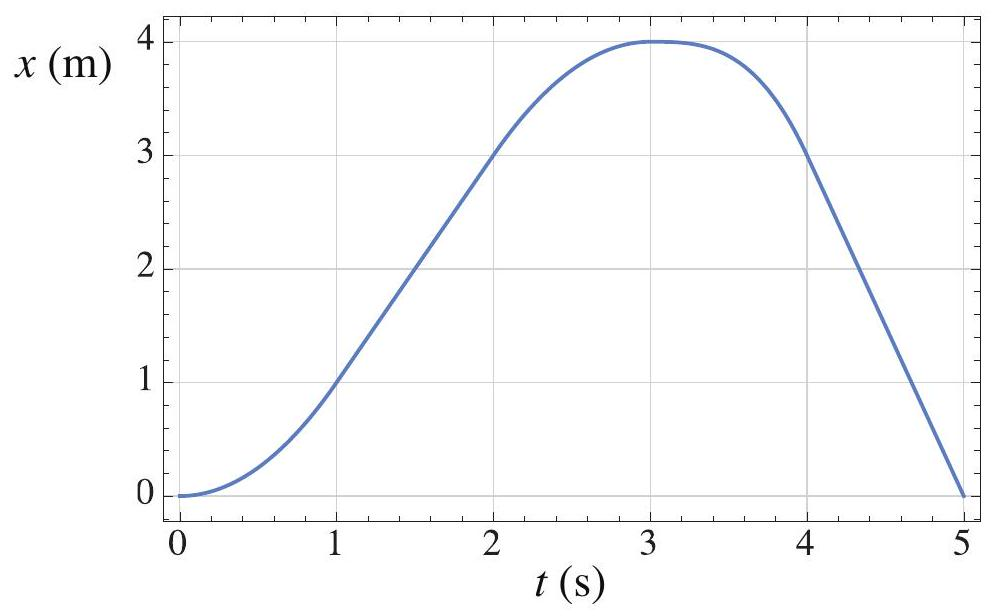
\includegraphics[max width=\textwidth]{2024_09_14_9969b06773f10b6936e8g-045}
\end{center}

The above figure is the position (in meters) versus time (in seconds) graph of an object in motion. Only the segments between $t=1 \mathrm{~s}$ and $t=2 \mathrm{~s}$, and between $t=4 \mathrm{~s}$ and $t=5 \mathrm{~s}$, are straight lines. The peak of the curve is at $t=3 \mathrm{~s}, x=4 \mathrm{~m}$.

Answer the following questions, and provide a brief justification for your answer in every case.\\
(a) At what time(s) is the object's velocity equal to zero?\\
(b) For what range(s) of times is the object moving with constant velocity?\\
(c) What is the object's position coordinate at $t=1 \mathrm{~s}$ ?\\
(d) What is the displacement of the object between $t=1 \mathrm{~s}$ and $t=4 \mathrm{~s}$ ?\\
(e) What is the distance traveled between $t=1 \mathrm{~s}$ and $t=4 \mathrm{~s}$ ?\\
(f) What is the instantaneous velocity of the object at $t=1.5 \mathrm{~s}$ ?\\
(g) What is its average velocity between $t=1 \mathrm{~s}$ and $t=3 \mathrm{~s}$ ?

\section*{Problem 2}
A particle is initially at $x_{i}=3 \mathrm{~m}, y_{i}=-5 \mathrm{~m}$, and after a while it is found at the coordinates $x_{f}=-4 \mathrm{~m}, y_{f}=2 \mathrm{~m}$.\\
(a) On the grid below (next page), draw the initial and final position vectors, and the displacement vector.\\
(b) What are the components of the displacement vector?\\
(c) What are the magnitude and direction of the displacement vector? (You can specify the direction by the angle it makes with either the positive $x$ or the positive $y$ axis.)

\begin{center}
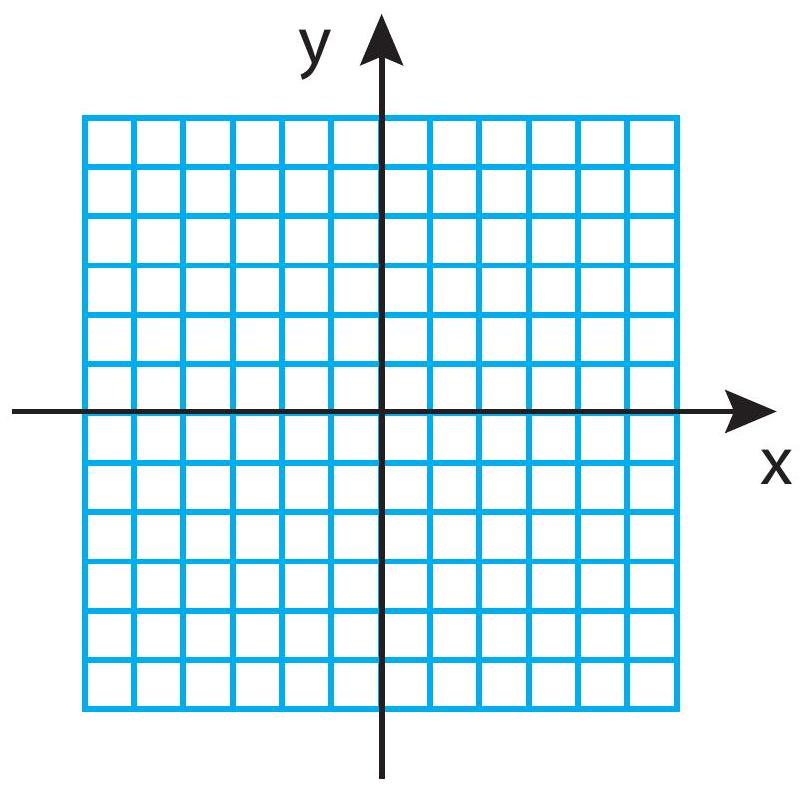
\includegraphics[max width=\textwidth]{2024_09_14_9969b06773f10b6936e8g-046}
\end{center}

\section*{Problem 3}
Marshall Dillon is riding at 30 mph after the robber of the Dodge City bank, who has a head start of 15 minutes, but whose horse can only make 25 mph on a good day. How long does it take for Dillon to catch up with the bad guy, and how far from Dodge City are they when this happens? (Assume the road is straight, for simplicity.)

\section*{Problem 4}
The picture below shows the velocity versus time graph of the first 21 seconds of a race between two friends, "Red" and "Green."\\
(a) Who is ahead at $t=10 \mathrm{~s}$, and by how much?\\
(b) Who passes the 100 m marker first?

\begin{center}
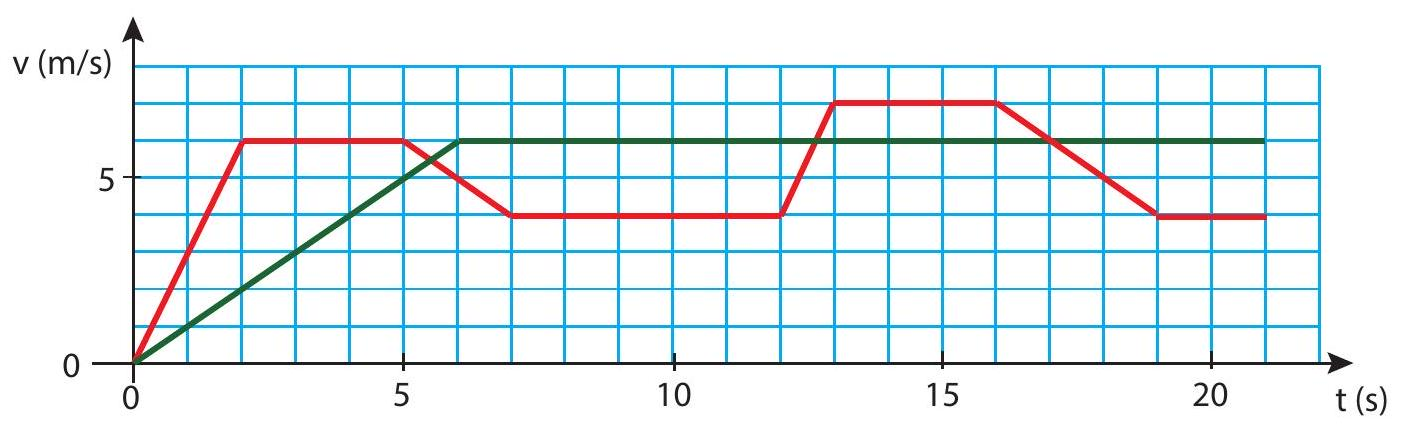
\includegraphics[max width=\textwidth]{2024_09_14_9969b06773f10b6936e8g-046(1)}
\end{center}

\section*{Problem 5}
You are trying to pass a truck on the highway. The truck is driving at 55 mph , so you speed up to 60 mph and move over to the left lane. If the truck is 17 m long, and your car is 3 m long\\
(a) how long does it take you to pass the truck completely?\\
(b) How far (along the highway) have you traveled in that time?

Note: to answer part (a) look at the problem from the perspective of the truck driver. How far are you going relative to him, and how far would it take you to cover 20 m at that speed?

\section*{Problem 6}
Suppose the position function of a particle moving in one dimension is given by


\begin{equation*}
x(t)=5+3 t+2 t^{2}-0.5 t^{3} \tag{1.30}
\end{equation*}


where the coefficients are such that the result will be in meters if you enter the time in seconds. What is the particle's velocity at $t=2 \mathrm{~s}$ ? There are two ways you can do this:

\begin{itemize}
  \item If you know calculus, calculate the derivative of (1.30) and evaluate it at $t=2 \mathrm{~s}$.
  \item If you do not yet know how to take derivatives, calculate the limit in the definition (1.8). That is to say, calculate $\Delta x / \Delta t$ with $t_{i}=2 \mathrm{~s}$ and $\Delta t$ equal, first, to 0.1 s , then to 0.01 s , and then to 0.001 s . You will need to keep more than the usual 4 decimals in the intermediate calculations if you want an accurate result, but you should still report only 3 significant digits in the final result.
\end{itemize}

\section*{Problem 7}
Suppose you are rowing across a river, as in Figure 1.7. Your speed is 2 miles per hour relative to the current, which is moving at a leisurely 1 mile per hour. If the river is 10 m wide,\\
(a) How far downstream do you end up?\\
(b) To row straight across you would need to have an upstream velocity component (relative to the current). How large would that be?\\
(c) If your rowing speed is still only 2 miles per hour, how long does it take you to row across the river now?

\section*{Chapter 2}
\section*{Acceleration}
\subsection*{2.1 The law of inertia}
There is something funny about motion with constant velocity: it is indistinguishable from rest. Of course, you can usually tell whether you are moving relative to something else. But if you are enjoying a smooth airplane ride, without looking out the window, you have no idea how fast you are moving, or even, indeed (if the flight is exceptionally smooth) whether you are moving at all. I am actually writing this on an airplane. The flight screen informs me that I am moving at 480 mph relative to the ground, but I do not feel anything like that: just a gentle rocking up and down and sideways that gives me no clue as to what my forward velocity is.

If I were to drop something, I know from experience that it would fall on a straight line - relative to me, that is. If it falls from my hand it will land at my feet, just as if we were all at rest. But we are not at rest. In the half second or so it takes for the object to fall, the airplane has moved forward 111 meters relative to the ground. Yet the (hypothetical) object I drop does not land 300 feet behind me! It moves forward with me as it falls, even though I am not touching it. It keeps its initial forward velocity, even though it is no longer in contact with me or anything connected to the airplane.\\
(At this point you might think that the object is still in contact with the air inside the plane, which is moving with the plane, and conjecture that maybe it is the air inside the plane that "pushes forward" on the object as it falls and keeps it from moving backwards. This is not necessarily a dumb idea, but a moment's reflection will convince you that it is impossible. We are all familiar with the way air pushes on things moving through it, and we know that the force an object experiences depends on its mass and its shape, so if that was what was happening, dropping objects of different masses and shapes I would see them falling in all kind of different ways-as I would, in fact, if I\\
were dropping things from rest outdoors in a strong wind. But that is not what we experience on an airplane at all. The air, in fact, has no effect on the forward motion of the falling object. It does not push it in any way, because it is moving at the same velocity. This, in fact, reinforces our previous conclusion: the object keeps its forward velocity while it is falling, in the absence of any external influence.)

This remarkable observation is one of the most fundamental principles of physics (yes, we have started to learn physics now!), which we call the law of inertia. It can be stated as follows: in the absence of any external influence (or force) acting on it, an object at rest will stay at rest, while an object that is already moving with some velocity will keep that same velocity (speed and direction of motion) - at least until it is, in fact, acted upon by some force.

Please let that sink in for a moment, before we start backtracking, which we have to do now on several accounts. First, I have used repeatedly the term "force," but I have not defined it properly. Or have I? What if I just said that forces are precisely any "external influences" that may cause a change in the velocity of an object? That will work, I think, until it is time to explore the concept in more detail, a few chapters from now.

Next, I need to draw your attention to the fact that the object I (hypothetically) dropped did not actually keep its total initial velocity: it only kept its initial forward velocity. In the downward direction, it was speeding up from the moment it left my hand, as would any other falling object (and as we shall see later in this chapter). But this actually makes sense in a certain way: there was no forward force, so the forward velocity remained constant; there was, however, a vertical force acting all along (the force of gravity), and so the object did speed up in that direction. This observation is, in fact, telling us something profound about the world's geometry: namely, that forces and velocities are vectors, and laws such as the law of inertia will typically apply to the vector as a whole, as well as to each component separately (that is to say, each dimension of space). This anticipates, in fact, the way we will deal, later on, with motion in two or more dimensions; but we do not need to worry about that for a few chapters still.

Finally, it is worth spending a moment reflecting on how radically the law of inertia seems to contradict our intuition about the way the world works. What it seems to be telling us is that, if we throw or push an object, it should continue to move forever with the same speed and in the same direction with which it set out - something that we know is certainly not true. But what's happening in "real life" is that, just because we have left something alone, it doesn't mean the world has left it alone. After we lose contact with the object, all sorts of other forces will continue to act on it. A ball we throw, for instance, will experience air resistance or drag (the same effect I was worrying about in that paragraph in parenthesis in the previous page), and that will slow it down. An object sliding on a surface will experience friction, and that will slow it down too. Perhaps the closest thing to the law of inertia in action that you may get to see is a hockey puck sliding on the ice: it is remarkable (perhaps even a bit frightening) to see how little it slows down, but even so the ice does a exert a (very small) frictional force that would bring the puck to a stop eventually.

This is why, historically, the law of inertia was not discovered until people started developing an appreciation for frictional forces, and the way they are constantly acting all around us to oppose the relative motion of any objects trying to slide past each other.

This mention of relative motion, in a way, brings us full circle. Yes, relative motion is certainly detectable, and for objects in contact it actually results in the occurrence of forces of the frictional, or drag, variety. But absolute (that is, without reference to anything external) motion with constant velocity is fundamentally undetectable. And in view of the law of inertia, it makes sense: if no force is required to keep me moving with constant velocity, it follows that as long as I am moving with constant velocity I should not be feeling any net force acting on me; nor would any other detection apparatus I might be carrying with me.

What we do feel in our bodies, and what we can detect with our inertial navigation systems (now you may start to guess why they are called "inertial"), is a change in our velocity, which is to say, our acceleration (to be defined properly in a moment). We rely, ultimately, on the law of inertia to detect accelerations: if my plane is shaking up and down, because of turbulence (as, in fact, it is right now!), the water in my cup may not stay put. Or, rather, the water may try to stay put (really, to keep moving, at any moment, with whatever velocity it has at that moment), but if the cup, which is connected to my hand which is connected, ultimately, to this bouncy plane, moves suddenly out from under it, not all of the water's parts will be able to adjust their velocities to the new velocity of the cup in time to prevent a spill.

This is the next very interesting fact about the physical world that we are about to discover: forces cause accelerations, or changes in velocity, but they do so in different degrees for different objects; and, moreover, the ultimate change in velocity takes time. The first part of this statement has to do with the concept of inertial mass, to be introduced in the next chapter; the second part we are going to explore right now, after a brief detour to define inertial reference frames.

\subsection*{2.1.1 Inertial reference frames}
The example I just gave you of what happens when a plane in flight experiences turbulence points to an important phenomenon, namely, that there may be times where the law of inertia may not seem to apply in a certain reference frame. By this I mean that an object that I left at rest, like the water in my cup, may suddenly start to move - relative to the reference frame coordinates - even though nothing and nobody is acting on it. More dramatically still, if a car comes to a sudden stop, the passengers may be "projected forward" - they were initially at rest relative to the car frame, but now they find themselves moving forward (always in the car reference frame), to the point that, if they are not wearing seat belts, they may end up hitting the dashboard, or the seat in front of them.

Again, nobody has pushed on them, and in fact what we can see in this case, from outside the car, is nothing but the law of inertia at work: the passengers were just keeping their initial velocity, when the car suddenly slowed down under and around them. So there is nothing wrong with the law of inertia, but there is a problem with the reference frame: if I want to describe the motion of objects in a reference frame like a plane being shaken up or a car that is speeding up or slowing down, I need to allow for the fact that objects may move - always relative to that frame - in an apparent violation of the law of inertia.

The way we deal with this in physics is by introducing the very important concept of an inertial reference frame, by which we mean a reference frame in which all objects will, at all times, be observed to move (or not move) in a way fully consistent with the law of inertia. In other words, the law of inertia has to hold when we use that frame's own coordinates to calculate the objects' velocities. This, of course, is what we always do instinctively: when I am on a plane I locate the various objects around me relative to the plane frame itself, not relative to the distant ground.

To ascertain whether a frame is inertial or not, we start by checking to see if the description of motion using that frame's coordinates obeys the law of inertia: does an object left at rest on the counter in the laboratory stay at rest? If set in motion, does it move with constant velocity on a straight line? The Earth's surface, as it turns out, is not quite a perfect inertial reference frame, but it is good enough that it made it possible for us to discover the law of inertia in the first place!

What spoils the inertial-ness of an Earth-bound reference frame is the Earth's rotation, which, as we shall see later, is an example of accelerated motion. In fact, if you think about the grossly non-inertial frames I have introduced above - the bouncy plane, the braking car-they all have this in common: that their velocities are changing; they are not moving with constant speed on a straight line.

So, once you have found an inertial reference frame, to decide whether another one is inertial or not is simple: if it is moving with constant velocity (relative to the first, inertial frame), then it is itself inertial; if not, it is not. I will show you how this works, formally, in a little bit (section 2.2.4, below), after I (finally!) get around to properly introducing the concept of acceleration.

It is a fundamental principle of physics that the laws of physics take the same form in all inertial reference frames. The law of inertia is, of course, an example of such a law. Since all inertial frames are moving with constant velocity relative to each other, this is another way to say that absolute motion is undetectable, and all motion is ultimately relative. Accordingly, this principle is known as the principle of relativity.

\subsection*{2.2 Acceleration}
\subsection*{2.2.1 Average and instantaneous acceleration}
Just as we defined average velocity in the previous chapter, using the concept of displacement (or change in position) over a time interval $\Delta t$, we define average acceleration over the time $\Delta t$ using the change in velocity:


\begin{equation*}
a_{a v}=\frac{\Delta v}{\Delta t}=\frac{v_{f}-v_{i}}{t_{f}-t_{i}} \tag{2.1}
\end{equation*}


Here, $v_{i}$ and $v_{f}$ are the initial and final velocities, respectively, that is to say, the velocities at the beginning and the end of the time interval $\Delta t$. As was the case with the average velocity, though, the average acceleration is a concept of somewhat limited usefulness, so we might as well proceed straight away to the definition of the instantaneous acceleration (or just "the" acceleration, without modifiers), through the same sort of limiting process by which we defined the instantaneous velocity:


\begin{equation*}
a=\lim _{\Delta t \rightarrow 0} \frac{\Delta v}{\Delta t} \tag{2.2}
\end{equation*}


Everything that we said in the previous chapter about the relationship between velocity and position can now be said about the relationship between acceleration and velocity. For instance (if you know calculus), the acceleration as a function of time is the derivative of the velocity as a function of time, which makes it the second derivative of the position function:


\begin{equation*}
a=\frac{d v}{d t}=\frac{d^{2} x}{d t^{2}} \tag{2.3}
\end{equation*}


(and if you do not know calculus yet, do not worry about the superscripts "2" on that last expression! It is just a weird notation that you will learn someday.)

Similarly, we can "read off" the instantaneous acceleration from a velocity versus time graph, by looking at the slope of the line tangent to the curve at any point. However, if what we are given is a position versus time graph, the connection to the acceleration is more indirect. Figure 2.1 (next page) provides you with such an example. See if you can guess at what points along this curve the acceleration is positive, negative, or zero.

The way to do this "from scratch," as it were, is to try to figure out what the velocity is doing, first, and infer the acceleration from that. Here is how that would go:

Starting at $t=0$, and keeping an eye on the slope of the $x$-vs- $t$ curve, we can see that the velocity starts at zero or near zero and increases steadily for a while, until $t$ is a little bit more than 2 s (let us say, $t=2.2 \mathrm{~s}$ for definiteness). That would correspond to a period of positive acceleration, since $\Delta v$ would be positive for every $\Delta t$ in that range.

\begin{center}
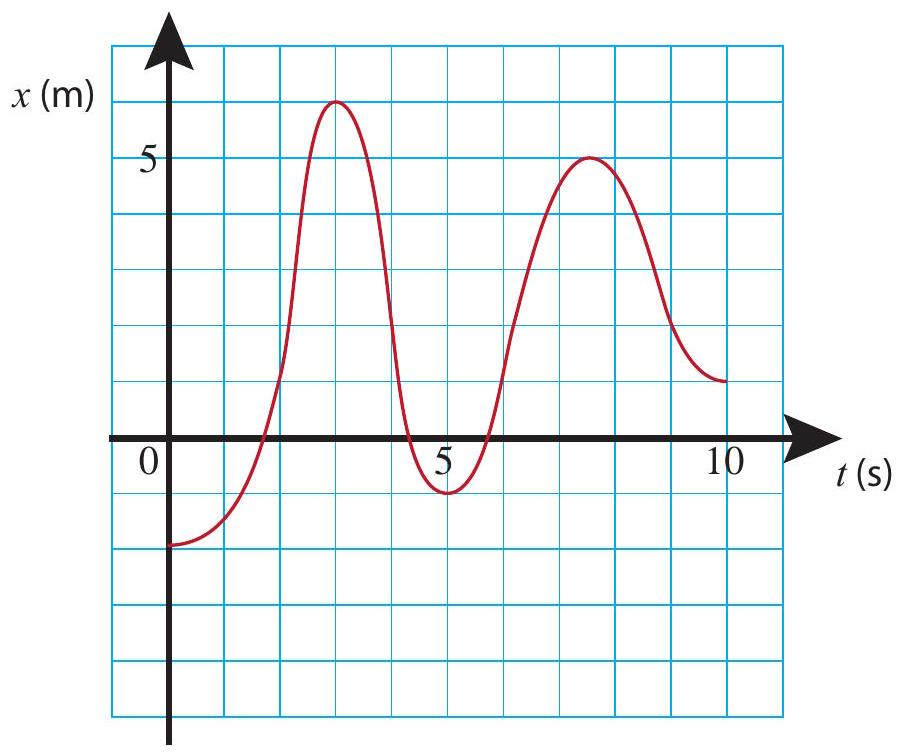
\includegraphics[max width=\textwidth]{2024_09_14_9969b06773f10b6936e8g-054}
\end{center}

Figure 2.1: A possible position vs. time graph for an object whose acceleration changes with time.

Between $t=2.2 \mathrm{~s}$ and $t=2.5 \mathrm{~s}$, as the object moves from $x=2 \mathrm{~m}$ to $x=4 \mathrm{~m}$, the velocity does not appear to change very much, and the acceleration would correspondingly be zero or near zero. Then, around $t=2.5 \mathrm{~s}$, the velocity starts to decrease noticeably, becoming (instantaneously) zero at $t=3 \mathrm{~s}(x=6 \mathrm{~m})$. That would correspond to a negative acceleration. Note, however, that the velocity afterwards continues to decrease, becoming more and more negative until around $t=4$ s. This also corresponds to a negative acceleration: even though the object is speeding up, it is speeding up in the negative direction, so $\Delta v$, and hence $a$, is negative for every time interval there. We conclude that $a<0$ for all times between $t=2.5 \mathrm{~s}$ and $t=4 \mathrm{~s}$.

Next, as we just look past $t=4 \mathrm{~s}$, something else interesting happens: the object is still going in the negative direction (negative velocity), but now it is slowing down. Mathematically, that corresponds to a positive acceleration, since the algebraic value of the velocity is in fact increasing (a number like -3 is larger than a number like -5 ). Another way to think about it is that, if we have less and less of a negative thing, our overall trend is positive. So the acceleration is positive all the way from $t=4 \mathrm{~s}$ through $t=5 \mathrm{~s}$ (where the velocity is instantaneously zero as the object's direction of motion reverses), and beyond, until about $t=6 \mathrm{~s}$, since between $t=5 \mathrm{~s}$ and $t=6 \mathrm{~s}$ the velocity is positive and growing.

You can probably figure out on your own now what happens after $t=6 \mathrm{~s}$, reasoning as I did above, but you may also have noticed a pattern that makes this kind of analysis a lot easier. The acceleration (as those with a knowledge of calculus may have understood already), being proportional to the second derivative of the function $x(t)$ with respect to $t$, is directly related to the curvature of the $x$-vs- $t$ graph. As figure 2.2 below shows, if the graph is concave (sometimes\\
called "concave upwards"), the acceleration is positive, whereas it is negative whenever the graph is convex (or "concave downwards"). It is (instantly) zero at those points where the curvature changes (which you may know as inflection points), as well as over stretches of time when the $x$-vs- $t$ graph is a straight line (motion with constant velocity).

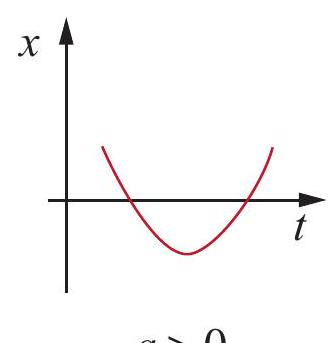
\includegraphics[max width=\textwidth, center]{2024_09_14_9969b06773f10b6936e8g-055(2)}\\
$a>0$

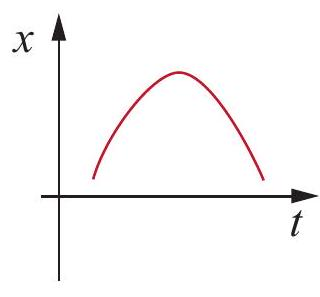
\includegraphics[max width=\textwidth, center]{2024_09_14_9969b06773f10b6936e8g-055}\\
$a<0$

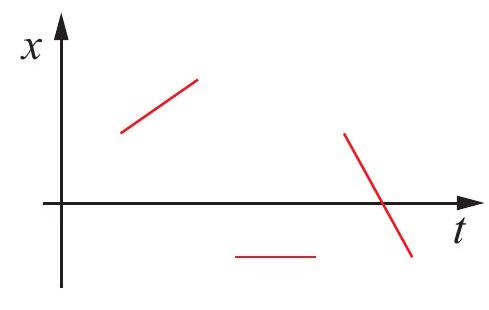
\includegraphics[max width=\textwidth, center]{2024_09_14_9969b06773f10b6936e8g-055(1)}\\
$a=0$\\
Figure 2.2: What the $x$-vs- $t$ curves look like for the different possible signs of the acceleration.

Figure 2.3 (in the next page) shows position, velocity, and acceleration versus time for a hypothetical motion case. Please study it carefully until every feature of every graph makes sense, relative to the other two! You will see many other examples of this in the homework and the lab.

Notice that, in all these figures, the sign of $x$ or $v$ at any given time has nothing to do with the sign of $a$ at that same time. It is true that, for instance, a negative $a$, if sustained for a sufficiently long time, will eventually result in a negative $v$ (as happens, for instance, in Fig. 2.3 over the interval from $t=1$ to $t=4 \mathrm{~s}$ ) but this may take a long time, depending on the size of $a$ and the initial value of $v$. The graphical clues to follow, instead, are: the acceleration is given by the slope of the tangent to the $v$-vs- $t$ curve, or the curvature of the $x$-vs- $t$ curve, as explained in Fig. 2.2; and the velocity is given by the slope of the tangent to the $x$-vs- $t$ curve.\\
(Note: To make the interpretation of Figure 2.3 simpler, I have chosen the acceleration to be "piecewise constant," that is to say, constant over extended time intervals and changing in value discontinuously from one interval to the next. This is physically unrealistic: in any real-life situation, the acceleration would be expected to change more or less smoothly from instant to instant. We will see examples of that later on, when we start looking at realistic models of collisions.)

\begin{center}
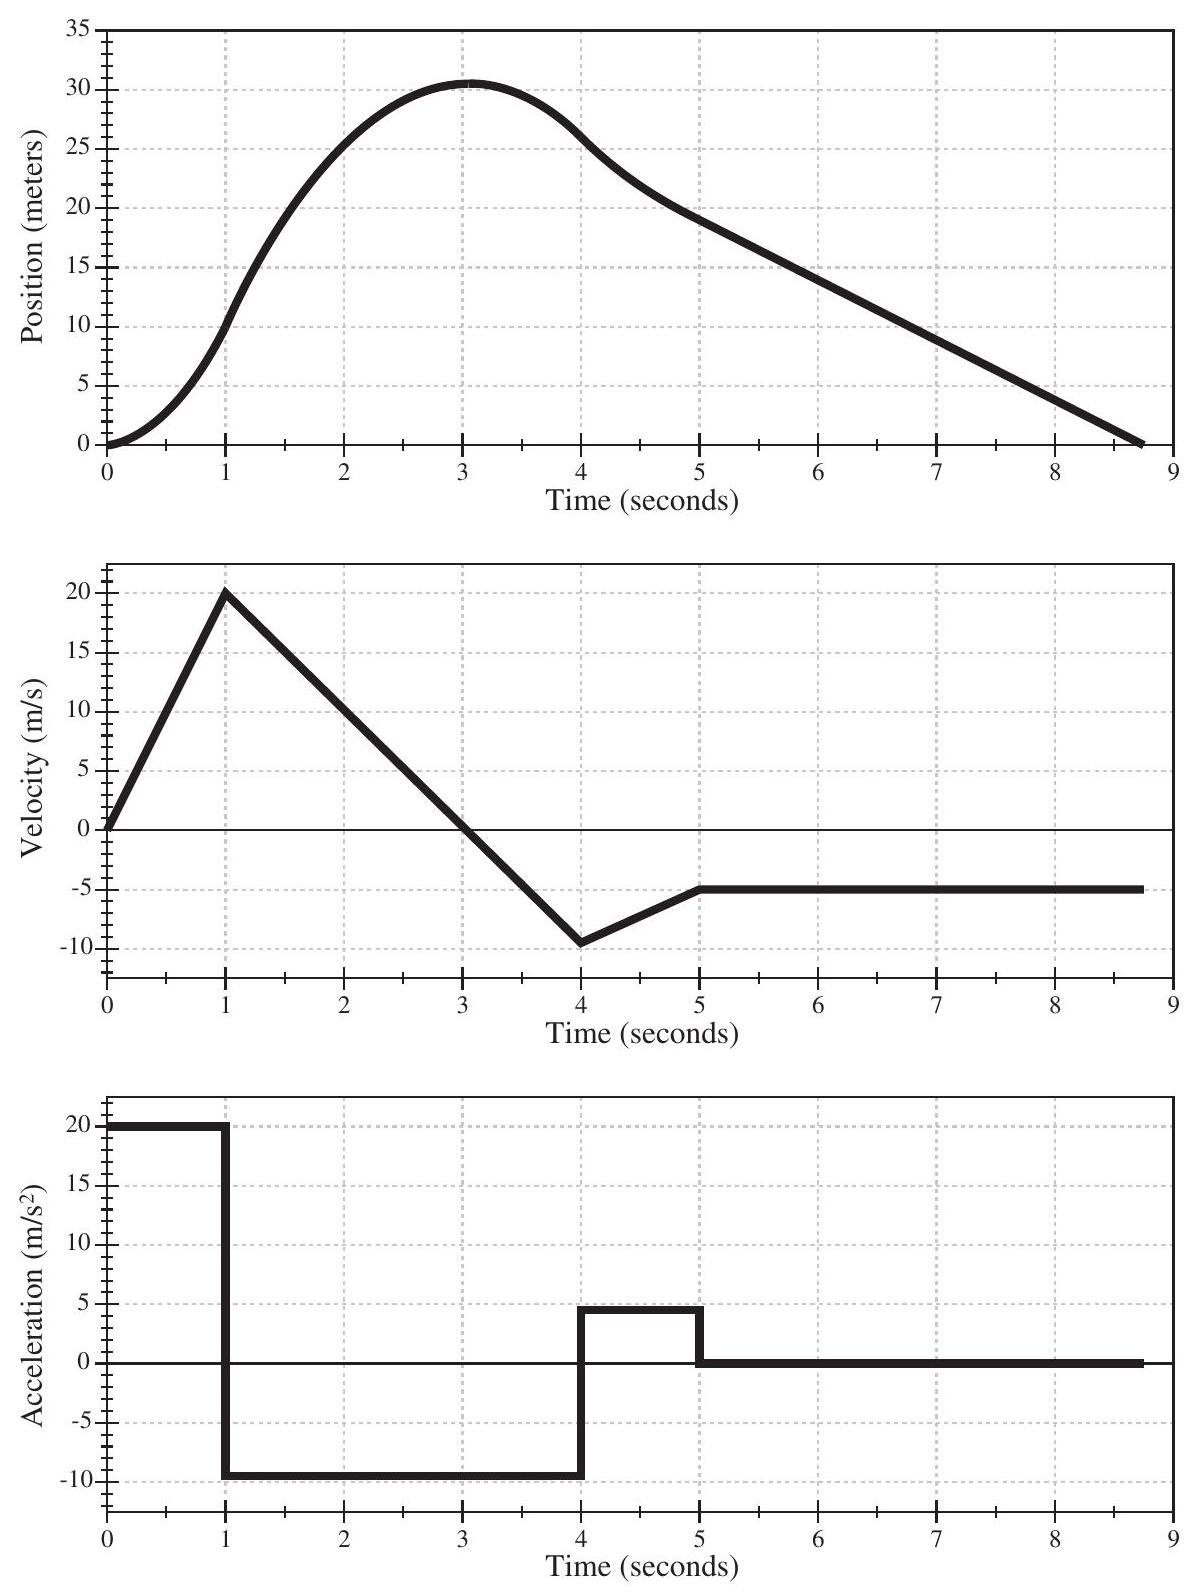
\includegraphics[max width=\textwidth]{2024_09_14_9969b06773f10b6936e8g-056}
\end{center}

Figure 2.3: Sample position, velocity and acceleration vs. time graphs for motion with piecewise-constant acceleration.

\subsection*{2.2.2 Motion with constant acceleration}
A particular kind of motion that is both relatively simple and very important in practice is motion with constant acceleration (see Figure 2.3 again for examples). If $a$ is constant, it means that the velocity changes with time at a constant rate, by a fixed number of $\mathrm{m} / \mathrm{s}$ each second. (These are, incidentally, the units of acceleration: meters per second per second, or $\mathrm{m} / \mathrm{s}^{2}$.) The change in velocity over a time interval $\Delta t$ is then given by


\begin{equation*}
\Delta v=a \Delta t \tag{2.4}
\end{equation*}


which can also be written


\begin{equation*}
v=v_{i}+a\left(t-t_{i}\right) \tag{2.5}
\end{equation*}


Equation (2.5) is the form of the velocity function ( $v$ as a function of $t$ ) for motion with constant acceleration. This, in turn, has to be the derivative with respect to time of the corresponding position function. If you know simple derivatives, then, you can verify that the appropriate form of the position function must be


\begin{equation*}
x=x_{i}+v_{i}\left(t-t_{i}\right)+\frac{1}{2} a\left(t-t_{i}\right)^{2} \tag{2.6}
\end{equation*}


or in terms of intervals,


\begin{equation*}
\Delta x=v_{i} \Delta t+\frac{1}{2} a(\Delta t)^{2} \tag{2.7}
\end{equation*}


Most often Eq. (2.6) is written with the implicit assumption that the initial value of $t$ is zero:


\begin{equation*}
x=x_{i}+v_{i} t+\frac{1}{2} a t^{2} \tag{2.8}
\end{equation*}


This is simpler, but not as general as Eq. (2.6). Always make sure that you know what conditions apply for any equation you decide to use!

As you can see from Eq. (2.5), for intervals during which the acceleration is constant, the velocity vs. time curve should be a straight line. Figure 2.3 (previous page) illustrates this. Equation (2.6), on the other hand, shows that for those same intervals the position vs. time curve should be a (portion of a) parabola, and again this can be seen in Figure 2.3 (sometimes, if the acceleration is small, the curvature of the graph may be hard to see; this happens in Figure 2.3 for the interval between $t=4 \mathrm{~s}$ and $t=5 \mathrm{~s})$.

The observation that $v$-vs- $t$ is a straight line when the acceleration is constant provides us with a simple way to derive Eq. (2.7), when combined with the result (from the end of the previous chapter) that the displacement over a time interval $\Delta t$ equals the area under the $v$-vs- $t$ curve for that time interval. Indeed, consider the situation shown in Figure 2.4. The total area under the segment shown is equal to the area of a rectangle of base $\Delta t$ and height $v_{i}$, plus the area of a\\
triangle of base $\Delta t$ and height $v_{f}-v_{i}$. Since $v_{f}-v_{i}=a \Delta t$, simple geometry immediately yields Eq. (2.7), or its equivalent (2.6).

\begin{center}
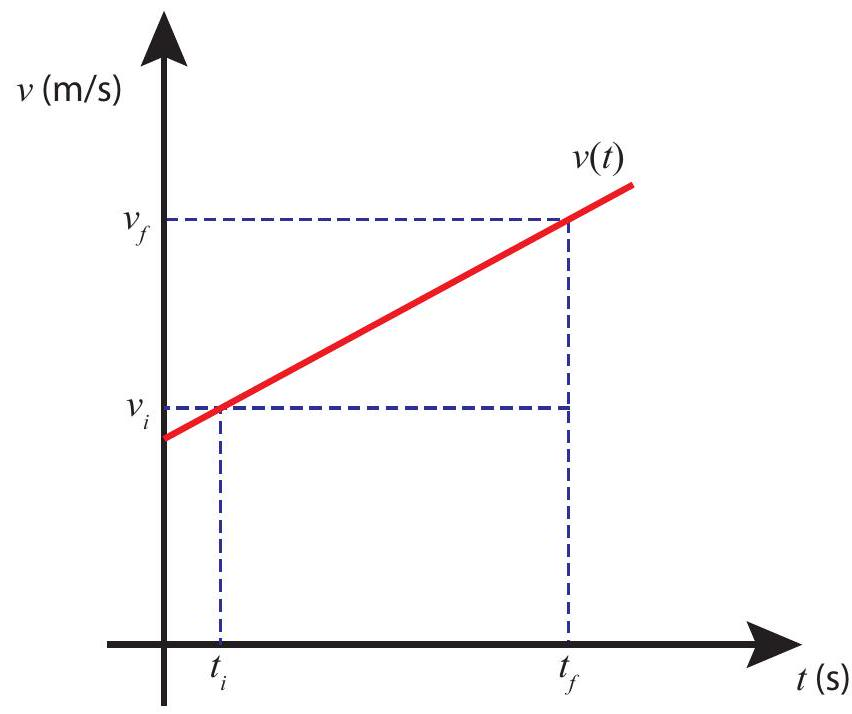
\includegraphics[max width=\textwidth]{2024_09_14_9969b06773f10b6936e8g-058}
\end{center}

Figure 2.4: Graphical way to find the displacement for motion with constant acceleration.

Lastly, consider what happens if we solve Eq. (2.4) for $\Delta t$ and substitute the result in (2.7). We get


\begin{equation*}
\Delta x=\frac{v_{i} \Delta v}{a}+\frac{(\Delta v)^{2}}{2 a} \tag{2.9}
\end{equation*}


Letting $\Delta v=v_{f}-v_{i}$, a little algebra yields


\begin{equation*}
v_{f}^{2}-v_{i}^{2}=2 a \Delta x \tag{2.10}
\end{equation*}


This is a handy little result that can also be seen to follow, more directly, from the work-energy theorems to be introduced in Chapter $7^{1}$.

\footnotetext{${ }^{1}$ In fact, equation (2.10) turns out to be so handy that you will probably find yourself using it over and over this semester, and you may even be tempted to use it for problems involving motion in two dimensions. However, unless you really know what you are doing, you should resist the temptation, since it is very easy to use (2.10) incorrectly when the acceleration and the displacement do not lie along the same line. You should use the appropriate form of a work-energy theorem instead.
}\subsection*{2.2.3 Acceleration as a vector}
In two (or more) dimensions we introduce the average acceleration vector


\begin{equation*}
\vec{a}_{a v}=\frac{\Delta \vec{v}}{\Delta t}=\frac{1}{\Delta t}\left(\vec{v}_{f}-\vec{v}_{i}\right) \tag{2.11}
\end{equation*}


whose components are $a_{a v, x}=\Delta v_{x} / \Delta t$, etc.. The instantaneous acceleration is then the vector given by the limit of Eq. (2.11) as $\Delta t \rightarrow 0$, and its components are, therefore, $a_{x}=d v_{x} / d t, a_{y}=d v_{y} / d t, \ldots$

Note that, since $\vec{v}_{i}$ and $\vec{v}_{f}$ in Eq. (2.11) are vectors, and have to be subtracted as such, the acceleration vector will be nonzero whenever $\vec{v}_{i}$ and $\vec{v}_{f}$ are different, even if, for instance, their magnitudes (which are equal to the object's speed) are the same. In other words, you have accelerated motion whenever the direction of motion changes, even if the speed does not.

As long as we are working in one dimension, I will follow the same convention for the acceleration as the one I introduced for the velocity in Chapter 1: namely, I will use the symbol $a$, without a subscript, to refer to the relevant component of the acceleration $\left(a_{x}, a_{y}, \ldots\right)$, and not to the magnitude of the vector $\vec{a}$.

\subsection*{2.2.4 Acceleration in different reference frames}
In Chapter 1 you saw that the following relation (Eq. (1.19)) holds between the velocities of a particle P measured in two different reference frames, A and B :


\begin{equation*}
\vec{v}_{A P}=\vec{v}_{A B}+\vec{v}_{B P} \tag{2.12}
\end{equation*}


What about the acceleration? An equation like (2.12) will hold for the initial and final velocities, and subtracting them we will get


\begin{equation*}
\Delta \vec{v}_{A P}=\Delta \vec{v}_{A B}+\Delta \vec{v}_{B P} \tag{2.13}
\end{equation*}


Now suppose that reference frame B moves with constant velocity relative to frame A. In that case, $\vec{v}_{A B, f}=\vec{v}_{A B, i}$, so $\Delta \vec{v}_{A B}=0$, and then, dividing Eq. (2.13) by $\Delta t$, and taking the limit $\Delta t \rightarrow 0$, we get


\begin{equation*}
\vec{a}_{A P}=\vec{a}_{B P} \quad\left(\text { for constant } \vec{v}_{A B}\right) \tag{2.14}
\end{equation*}


So, if two reference frames are moving at constant velocity relative to each other, observers in both frames measure the same acceleration for any object they might both be tracking.

The result (2.14) means, in particular, that if we have an inertial frame then any frame moving at constant velocity relative to it will be inertial too, since the respective observers' measurements\\
will agree that an object's velocity does not change (otherwise put, its acceleration is zero) when no forces act on it. Conversely, an accelerated frame will not be an inertial frame, because Eq. (2.14) will not hold. This is consistent with the examples I mentioned in Section 2.1 (the bouncing plane, the car coming to a stop). Another example of a non-inertial frame would be a car going around a curve, even if it is going at constant speed, since, as I just pointed out above, this is also an accelerated system. This is confirmed by the fact that objects in such a car tend to move - relative to the car-towards the outside of the curve, even though no actual force is acting on them.

\subsection*{2.3 Free fall}
An important example of motion with (approximately) constant acceleration is provided by free fall near the surface of the Earth. We say that an object is in "free fall" when the only force acting on it is the force of gravity (the word "fall" here may be a bit misleading, since the object could actually be moving upwards some of the time, if it has been thrown straight up, for instance). The space station is in free fall, but because it is nowhere near the surface of the earth its direction of motion (and hence its acceleration, regarded as a two-dimensional vector) is constantly changing. Right next to the surface of the earth, on the other hand, the planet's curvature is pretty much negligible and gravity provides an approximately constant, vertical acceleration, which, in the absence of other forces, turns out to be the same for every object, regardless of its size, shape, or weight.

The above result - that, in the absence of other forces, all objects should fall to the earth at the same rate, regardless of how big or heavy they are - is so contrary to our common experience that it took many centuries to discover it. The key, of course, as with the law of inertia, is to realize that, under normal circumstances, frictional forces are, in fact, acting all the time, so an object falling through the atmosphere is never really in "free" fall: there is always, at a minimum, and in addition to the force of gravity, an air drag force that opposes its motion. The magnitude of this force does depend on the object's size and shape (basically, on how "aerodynamic" the object is); and thus a golf ball, for instance, falls much faster than a flat sheet of paper. Yet, if you crumple up the sheet of paper till it has the same size and shape as the golf ball, you can see for yourself that they do fall at approximately the same rate! The equality can never be exact, however, unless you get rid completely of air drag, either by doing the experiment in an evacuated tube, or (in a somewhat extreme way), by doing it on the surface of the moon, as the Apollo 15 astronauts did with a hammer and a feather back in $1971^{2}$.

This still leaves us with something of a mystery, however: the force of gravity is the only force known to have the property that it imparts all objects the same acceleration, regardless of their mass or constitution. A way to put this technically is that the force of gravity on an object is

\footnotetext{${ }^{2}$ The video of this is available online: \href{https://www.youtube.com/watch?v=oYEgdZ3iEKA}{https://www.youtube.com/watch?v=oYEgdZ3iEKA}. It is, however, pretty low resolution and hard to see. A very impressive modern-day demonstration involving feathers and a bowling ball in a completely evacuated (airless) room is available here: \href{https://www.youtube.com/watch?v=E43-CfukEgs}{https://www.youtube.com/watch?v=E43-CfukEgs}.
}
proportional to that object's inertial mass, a quantity that we will introduce properly in the next chapter. For the time being, we will simply record here that this acceleration, near the surface of the earth, has a magnitude of approximately $9.8 \mathrm{~m} / \mathrm{s}^{2}$, a quantity that is denoted by the symbol $g$. Thus, if we take the upwards direction as positive (as is usually done), we get for the acceleration of an object in free fall $a=-g$, and the equations of motion become\\
\$\$

\begin{gather*}
\Delta v=-g \Delta t  \tag{2.15}\\
\Delta y=v_{i} \Delta t-\frac{1}{2} g(\Delta t)^{2} \tag{2.16}
\end{gather*}

\$\$\\
where I have used $y$ instead of $x$ for the position coordinate, since that is a more common choice for a vertical axis. Note that we could as well have chosen the downward direction as positive, and that may be a more natural choice in some problems. Regardless, the quantity $g$ is always defined to be positive: $g=9.8 \mathrm{~m} / \mathrm{s}^{2}$. The acceleration, then, is $g$ or $-g$, depending on which direction we take to be positive.

In practice, the value of $g$ changes a little from place to place around the earth, for various reasons (it is somewhat sensitive to the density of the ground below you, and it decreases as you climb higher away from the center of the earth). In a later chapter we will see how to calculate the value of $g$ from the mass and radius of the earth, and also how to calculate the equivalent quantity for other planets.

In the meantime, we can use equations like (2.15) and (2.16) (as well as (2.10), with the appropriate substitutions) to answer a number of interesting questions about objects thrown or dropped straight up or down (always, of course, assuming that air drag is negligible). For instance, back at the beginning of this chapter I mentioned that if I dropped an object it might take about half a second to hit the ground. If you use Eq. (2.16) with $v_{i}=0$ (since I am dropping the object, not throwing it down, its initial velocity is zero), and substitute $\Delta t=0.5 \mathrm{~s}$, you get $\Delta y=1.23 \mathrm{~m}$ (about 4 feet). This is a reasonable height from which to drop something.

On the other hand, you may note that half a second is not a very long time in which to make accurate observations (especially if you do not have modern electronic equipment), and as a result of that there was considerable confusion for many centuries as to the precise way in which objects fell. Some people believed that the speed did increase in some way as the object fell, while others appear to have believed that an object dropped would "instantaneously" (that is, at soon as it left your hand) acquire some speed and keep that unchanged all the way down. In reality, in the presence of air drag, what happens is a combination of both: initially the speed increases at an approximately constant rate (free, or nearly free fall), but the drag force increases with the speed as well, until eventually it balances out the force of gravity, and from that point on the speed does not increase anymore: we say that the object has reached "terminal velocity." Some objects reach terminal velocity almost instantly, whereas others (the more "aerodynamic" ones) may take a long time to do so. This accounts for the confusion that prevailed before Galileo's experiments in the early 1600 's.

Galileo's main insight, on the theoretical side, was the realization that it was necessary to separate clearly the effect of gravity and the effect of the drag force. Experimentally, his big idea was to use an inclined plane to slow down the "fall" of an object, so as to make accurate measurements possible (and also, incidentally, reduce the air drag force!). These "inclined planes" were just basically ramps down which he sent small balls (like marbles) rolling. By changing the steepness of the ramp he could control how slowly the balls moved. He reasoned that, ultimately, the force that made the balls go down was essentially the same force of gravity, only not the whole force, but just a fraction of it. Today we know that, in fact, an object sliding (not rolling!) up or down on a frictionless incline will experience an acceleration directed downwards along the incline and with a magnitude equal to $g \sin \theta$, where $\theta$ is the angle that the slope makes with the horizontal:


\begin{equation*}
a=g \sin \theta \quad \text { (inclined plane, taking downwards to be positive) } \tag{2.17}
\end{equation*}


(for some reason, it seems more natural, when dealing with inclined planes, to take the downward direction as positive!). Equation (2.17) makes sense in the two extreme cases in which the plane is completely vertical $\left(\theta=90^{\circ}, a=g\right)$ and completely horizontal $\left(\theta=0^{\circ}, a=0\right)$. For intermediate values, you will carry out experiments in the lab to verify this result.

We will show, in a later chapter, how Eq. (2.17) comes about from a careful consideration of all the forces acting on the object; we will also see, later on, how it needs to be modified for the case of a rolling, rather than a sliding, object. This modification does not affect Galileo's main conclusion, which was, basically, that the natural falling motion in the absence of friction or drag forces is motion with constant acceleration (at least, near the surface of the earth, where $g$ is constant to a very good approximation).

\subsection*{2.4 In summary}
\begin{enumerate}
  \item The law of inertia states that, if no external influences (forces) are acting on an object, then, if the object is initially at rest it will stay at rest, and if it is initially moving it will continue to move with constant velocity (unchanging speed and direction).
  \item Reference frames in which the law of inertia is seen to hold (when the velocities of objects are calculated from their coordinates in that frame) are called inertial. A reference frame that is moving at constant velocity relative to an inertial frame is also an inertial frame. Conversely, accelerated reference frames are non-inertial.
  \item Motion with constant velocity is fundamentally indistinguishable from no motion at all (i.e., rest). As long as the velocity (of the objects involved) does not change, only relative motion can be detected. This is known as the principle of relativity. Another way to state it is that the laws of physics must take the same form in all inertial reference frames (so you cannot single out one as being in "absolute rest" or "absolute motion").
  \item Changes in velocity are detectable, and, by (1) above, are evidence of unbalanced forces acting on an object.
  \item The rate of change of an object's velocity is the object's acceleration: the average acceleration over a time interval $\Delta t$ is $a_{a v}=\Delta v / \Delta t$, and the instantaneous acceleration at a time $t$ is the limit of the average acceleration calculated for successively shorter time intervals $\Delta t$, all with the same initial time $t_{i}=t$. Mathematically, this means the acceleration is the derivative of the velocity function, $a=d v / d t$.
  \item In a velocity versus time graph, the acceleration can be read from the slope of the line tangent to the curve (just like the velocity in a position versus time graph).
  \item In a position versus time graph, the regions with positive acceleration correspond to a concave curvature (like a parabola opening up), and those with negative acceleration correspond to a convex curvature (like a parabola opening down). Points of inflection (where the curvature changes) and straight lines correspond to points where the acceleration is zero.
  \item The basic equations used to describe motion with constant acceleration are (2.4), (2.7) and (2.10) above. Alternative forms of these are also provided in the text.
  \item In more than one dimension, a change in the direction of the velocity vector results in a nonzero acceleration, even if the object's speed does not change.
  \item An object is said to be in free fall when the only force acting on it is gravity. All objects in free fall experience the same acceleration at the same point in their motion, regardless of their mass or composition. Near the surface of the earth, this acceleration is approximately constant and has a magnitude $g=9.8 \mathrm{~m} / \mathrm{s}^{2}$.
  \item An object sliding on a frictionless inclined plane experiences (if air drag is negligible) an acceleration directed downward along the incline and with a magnitude $g \sin \theta$, where $\theta$ is the angle the incline makes with the horizontal.
\end{enumerate}

\subsection*{2.5 Examples}
\subsection*{2.5.1 Motion with piecewise constant acceleration}
Construct the position vs. time, velocity vs. time, and acceleration vs. time graphs for the motion described below. For each of the intervals (a)-(d) you'll need to figure out the position (height) and velocity of the rocket at the beginning and the end of the interval, and the acceleration for the interval. In addition, for interval (b) you need to figure out the maximum height reached by the rocket and the time at which it occurs. For interval (d) you need to figure out its duration, that is to say, the time at which the rocket hits the ground.\\
(a) A rocket is shot upwards, accelerating from rest to a final velocity of $20 \mathrm{~m} / \mathrm{s}$ in 1 s as it burns its fuel. (Treat the acceleration as constant during this interval.)\\
(b) From $t=1 \mathrm{~s}$ to $t=4 \mathrm{~s}$, with the fuel exhausted, the rocket flies under the influence of gravity alone. At some point during this time interval (you need to figure out when!) it stops climbing and starts falling.\\
(c) At $t=4 \mathrm{~s}$ a parachute opens, suddenly causing an upwards acceleration (again, treat it as constant) lasting 1 s ; at the end of this interval, the rocket's velocity is $5 \mathrm{~m} / \mathrm{s}$ downwards.\\
(d) The last part of the motion, with the parachute deployed, is with constant velocity of $5 \mathrm{~m} / \mathrm{s}$ downwards until the rocket hits the ground.

\section*{Solution:}
(a) For this first interval (for which I will use a subscript " 1 " throughout) we have


\begin{equation*}
\Delta y_{1}=\frac{1}{2} a_{1}\left(\Delta t_{1}\right)^{2} \tag{2.18}
\end{equation*}


using Eq. (2.6) for motion with constant acceleration with zero initial velocity (I am using the variable $y$, instead of $x$, for the vertical coordinate; this is more or less customary, but, of course, I could have used $x$ just as well).

Since the acceleration is constant, it is equal to its average value:

$$
a_{1}=\frac{\Delta v}{\Delta t}=20 \frac{\mathrm{m}}{\mathrm{s}^{2}}
$$

Substituting this into (2.18) we get the height at $t=1 \mathrm{~s}$ is 10 m . The velocity at that time, of course, is $v_{f 1}=20 \mathrm{~m} / \mathrm{s}$, as we were told in the statement of the problem.\\
(b) This part is free fall with initial velocity $v_{i 2}=20 \mathrm{~m} / \mathrm{s}$. To find how high the rocket climbs, use Eq. (2.15) in the form $v_{\text {top }}-v_{i 2}=-g\left(t_{\text {top }}-t_{i 2}\right)$, with $v_{\text {top }}=0$ (as the rocket climbs, its velocity decreases, and it stops climbing when its velocity is zero). This gives us $t_{\text {top }}=3.04 \mathrm{~s}$ as the time at\\
which the rocket reaches the top of its trajectory, and then starts coming down. The corresponding displacement is, by Eq. (2.16),

$$
\Delta y_{\text {top }}=v_{i 2}\left(t_{t o p}-t_{i 2}\right)-\frac{1}{2} g\left(t_{t o p}-t_{i 2}\right)^{2}=20.4 \mathrm{~m}
$$

so the maximum height it reaches is 30.4 m .\\
At the end of the full 3 -second interval, the rocket's displacement is

$$
\Delta y_{2}=v_{i 2} \Delta t_{2}-\frac{1}{2} g\left(\Delta t_{2}\right)^{2}=15.9 \mathrm{~m}
$$

(so its height is 25.9 m above the ground), and the final velocity is

$$
v_{f 2}=v_{i 2}-g \Delta t_{2}=-9.43 \frac{\mathrm{m}}{\mathrm{s}}
$$

(c) The acceleration for this part is $\left(v_{f 3}-v_{i 3}\right) / \Delta t_{3}=(-5+9.43) / 1=4.43 \mathrm{~m} / \mathrm{s}^{2}$. Note the positive sign. The displacement is

$$
\Delta y_{3}=-9.43 \times 1+\frac{1}{2} \times 4.43 \times 1^{2}=-7.22 \mathrm{~m}
$$

so the final height is $25.9-7.21=18.7 \mathrm{~m}$.\\
(d) This is just motion with constant speed to cover 18.7 m at $5 \mathrm{~m} / \mathrm{s}$. The time it takes is 3.74 s .

The graphs for this motion are shown earlier in the chapter, in Figure 2.3.

\subsection*{2.6 Problems}
\section*{Problem 1}
You get on your bicycle and ride it with a constant acceleration of $0.5 \mathrm{~m} / \mathrm{s}^{2}$ for 20 s . After that, you continue riding at a constant velocity for a distance of 200 m . Finally, you slow to a stop, with a constant acceleration, over a distance of 20 m .

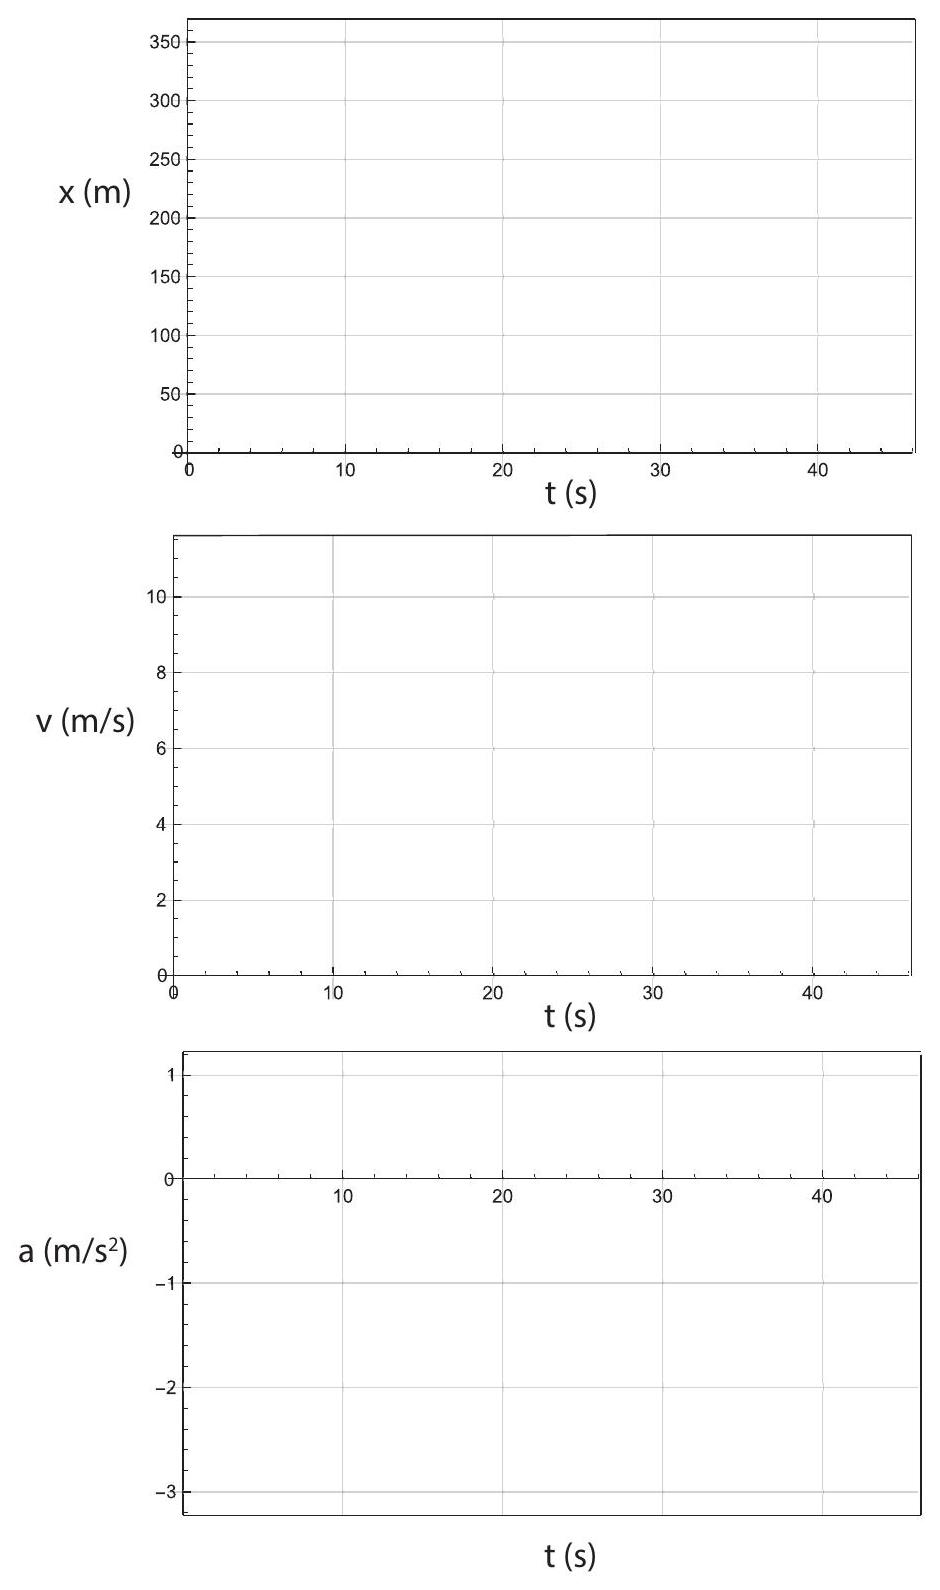
\includegraphics[max width=\textwidth, center]{2024_09_14_9969b06773f10b6936e8g-066}\\
(a) How far did you travel while you were accelerating at $0.5 \mathrm{~m} / \mathrm{s}^{2}$, and what was your velocity at the end of that interval?\\
(b) After that, how long did it take you to cover the next 200 m ?\\
(c) What was your acceleration while you were slowing down to a stop, and how long did it take you to come to a stop?\\
(d) Considering the whole trip, what was your average velocity?\\
(e) Plot the position versus time, velocity versus time, and acceleration versus time graphs for the whole trip, in the grids provided above. Values at the beginning and end of each interval must be exact. Slopes and curvatures must be represented accurately. Do not draw any of the curves beyond the time the rider stops (or, if you do, make sure what you draw makes sense!).

\section*{Problem 2}
You throw an object straight upwards and catch it again, when it comes down to the same initial height, 2 s later.\\
(a) How high did it rise above its initial height?\\
(b) With what initial speed did you throw it?\\
(Note: for this problem you should use the fact that, if air drag is negligible, the object will return to its initial height with the same speed it had initially.)

\section*{Problem 3}
You are trying to catch up with a car that is in front of you on the highway. Initially you are both moving at $25 \mathrm{~m} / \mathrm{s}$, and the distance between you is 100 m . You step on the gas and sustain a constant acceleration for a time $\Delta t=30 \mathrm{~s}$, at which point you have pulled even with the other car.\\
(a) What is $25 \mathrm{~m} / \mathrm{s}$, in miles per hour?\\
(b) What was your acceleration over the 30 s time interval?\\
(c) How fast were you going when you caught up with the other car?

\section*{Problem 4}
Go back to Problem 4 of Chapter 1, and use the information in the figure to draw an accurate position vs. time graph for both runners.

\section*{Problem 5}
A child on a sled slides (starting from rest) down an icy slope that makes an angle of $15^{\circ}$ with the horizontal. After sliding 20 m down the slope, the child enters a flat, slushy region, where she slides for 2.0 s with a constant negative acceleration of $-1.5 \mathrm{~m} / \mathrm{s}^{2}$ with respect to her direction of motion. She then slides up another icy slope that makes a $20^{\circ}$ angle with the horizontal.\\
(a) How fast was the child going when she reached the bottom of the first slope? How long did it take her to get there?\\
(b) How long was the flat stretch at the bottom?\\
(c) How fast was the child going as she started up the second slope?\\
(d) How far up the second slope did she slide?

\section*{Chapter 3}
\section*{Momentum and Inertia}
\subsection*{3.1 Inertia}
In everyday language, we speak of something or someone "having a large inertia" to mean, essentially, that they are very difficult to set in motion. This usage of the word "inertia" is consistent with the "law of inertia" we introduced in the previous chapter (which states, among other things, that an object at rest, if left to itself, will just remain at rest), but it goes a bit beyond that by trying to quantify just how hard it may be to get the object to move.

We do know, from experience, that lighter objects are easier to set in motion than heavier objects, but most of us probably have an intuition that gravity (the force that pulls an object towards the earth and hence determines its weight) is not involved in an essential way here. Imagine, for instance, the difference between slapping a volleyball and a bowling ball. It is not hard to believe that the latter would hurt as much if we did it while floating in free fall in the space station (in a state of effective "weightlessness") as if we did it right here on the surface of the earth. In other words, it is not (necessarily) how heavy something feels, but just how massive it is.

But just what is this "massiveness" quality that we associate intuitively with a large inertia? Is there a way (other than resorting to the weight again) to assign to it a numerical value?

\subsection*{3.1.1 Relative inertia and collisions}
One possible way to determine the relative inertias of two objects, conceptually, at least, is to try to use one of them to set the other one in motion. Most of us are familiar with what happens\\
when two identical objects (presumably, therefore, having the same inertia) collide: if the collision is head-on (so the motion, before and after, is confined to a straight line), they basically exchange velocities. For instance, a billiard ball hitting another one will stop dead and the second one will set off with the same speed as the first one. The toy sometimes called "Newton's balls" or "Newton's cradle" also shows this effect. Intuitively, we understand that what it takes to stop the first ball is exactly the same as it would take to set the second one in motion with the same velocity.

But what if the objects colliding have different inertias? We expect that the change in their velocities as a result of the collision will be different: the velocity of the object with the largest inertia will not change very much, and conversely, the change in the velocity of the object with the smallest inertia will be comparatively larger. A velocity vs. time graph for the two objects might look somewhat like the one sketched in Fig. 3.1.

\begin{center}
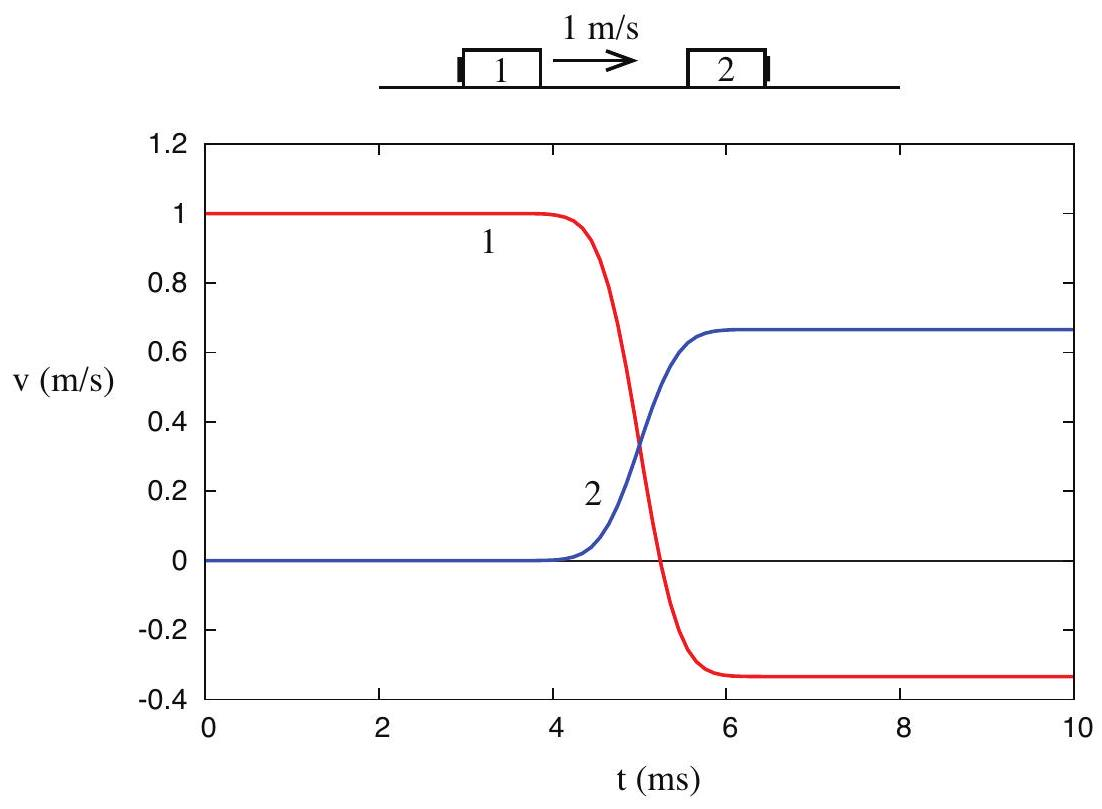
\includegraphics[max width=\textwidth]{2024_09_14_9969b06773f10b6936e8g-070}
\end{center}

Figure 3.1: An example of a velocity vs. time graph for a collision of two objects with different inertias.

In this picture, object 1 , initially moving with velocity $v_{1 i}=1 \mathrm{~m} / \mathrm{s}$, collides with object 2 , initially at rest. After the collision, which here is assumed to take a millisecond or so, object 1 actually bounces back, so its final velocity is $v_{1 f}=-1 / 3 \mathrm{~m} / \mathrm{s}$, whereas object 2 ends up moving to the right with velocity $v_{2 f}=2 / 3 \mathrm{~m} / \mathrm{s}$. So the change in the velocity of object 1 is $\Delta v_{1}=v_{1 f}-v_{1 i}=-4 / 3 \mathrm{~m} / \mathrm{s}$, whereas for object 2 we have $\Delta v_{2}=v_{2 f}-v_{2 i}=2 / 3 \mathrm{~m} / \mathrm{s}$.

It is tempting to use this ratio, $\Delta v_{1} / \Delta v_{2}$, as a measure of the relative inertia of the two objects, only we'd want to use it upside down and with the opposite sign: that is, since $\Delta v_{2} / \Delta v_{1}=-1 / 2$ we would say that object 2 has twice the inertia of object 1 . But then we have to ask: is this a\\
reliable, repeatable measure? Will it work for any kind of collision (within reason, of course: we clearly need to stay in one dimension, and eliminate external influences such as friction), and for any initial velocity?

To begin with, we have reason to expect that it does not matter whether we shoot object 1 towards object 2 or object 2 towards object 1, because we learned in the previous chapter that only relative motion is detectable, and the relative motion is the same in both cases. Consider, for instance, what the collision in Figure 3.1 appears like to a hypothetical observer moving along with object 1, at 1 $\mathrm{m} / \mathrm{s}$. To him, object 1 appears to be at rest, and it is object 2 that is coming towards him, with a velocity of $-1 \mathrm{~m} / \mathrm{s}$. To see what the outcome of the collision looks like to him, just add the same $-1 \mathrm{~m} / \mathrm{s}$ to the final velocities we obtained before: object 1 will end up moving at $v_{1 f}=-4 / 3 \mathrm{~m} / \mathrm{s}$, and object 2 would move at $v_{2 f}=-1 / 3 \mathrm{~m} / \mathrm{s}$, and we would have a situation like the one shown in Figure 3.2, where both curves have simply been shifted down by $1 \mathrm{~m} / \mathrm{s}$ :

\begin{center}
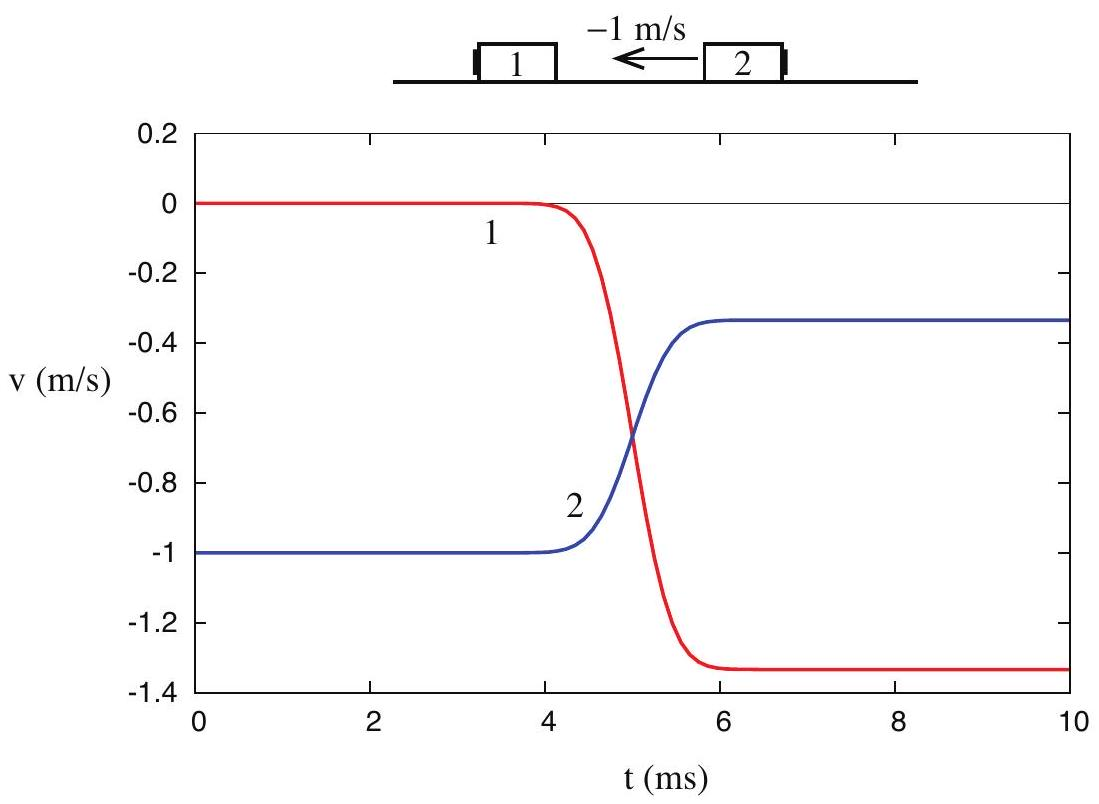
\includegraphics[max width=\textwidth]{2024_09_14_9969b06773f10b6936e8g-071}
\end{center}

Figure 3.2: Another example (really the same collision as in Figure 1, only as seen by an observer initially moving to the right at $1 \mathrm{~m} / \mathrm{s})$.

But then, this is exactly what we should expect to find also in our laboratory if we actually did send the second object at $1 \mathrm{~m} / \mathrm{s}$ towards the first one sitting at rest. All the individual velocities have changed relative to Figure 3.1, but the velocity changes, $\Delta v_{1}$ and $\Delta v_{2}$, are clearly still the same, and therefore so is our (tentative) measure of the objects' relative inertia.

Clearly, the same argument can be used to conclude that the same result will be obtained when both objects are initially moving towards each other, as long as their relative velocity is the same as\\
in these examples, namely, $1 \mathrm{~m} / \mathrm{s}$. However, unless we do the experiments we cannot really predict what will happen if we increase (or decrease) their relative velocity. In fact, we could imagine smashing the two objects at very high speed, so they might even become seriously mangled in the process. Yet, experimentally (and this is not at all an obvious result!), we would still find the same value of $-1 / 2$ for the ratio $\Delta v_{2} / \Delta v_{1}$, at least as long as the collision is not so violent that the objects actually break up into pieces.

Perhaps the most surprising result of our experiments would be the following: imagine that the objects have a "sticky" side (for instance, the small black rectangles shown in the pictures could be strips of Velcro), and we turn them around so that when they collide they will end up stuck to each other. In this case (which, as we shall see later, is termed a completely inelastic collision), the $v$-vs- $t$ graph might look like Figure 3.3 below.

Now the two objects end up moving together to the right, fairly slowly: $v_{1 f}=v_{2 f}=1 / 3 \mathrm{~m} / \mathrm{s}$. The velocity changes are $\Delta v_{1}=-2 / 3 \mathrm{~m} / \mathrm{s}$ and $\Delta v_{2}=1 / 3 \mathrm{~m} / \mathrm{s}$, both of which are different from what they were before, in Figs. 3.1 and 3.2: yet, the ratio $\Delta v_{2} / \Delta v_{1}$ is still equal to $-1 / 2$, just as in all the previous cases.

\begin{center}
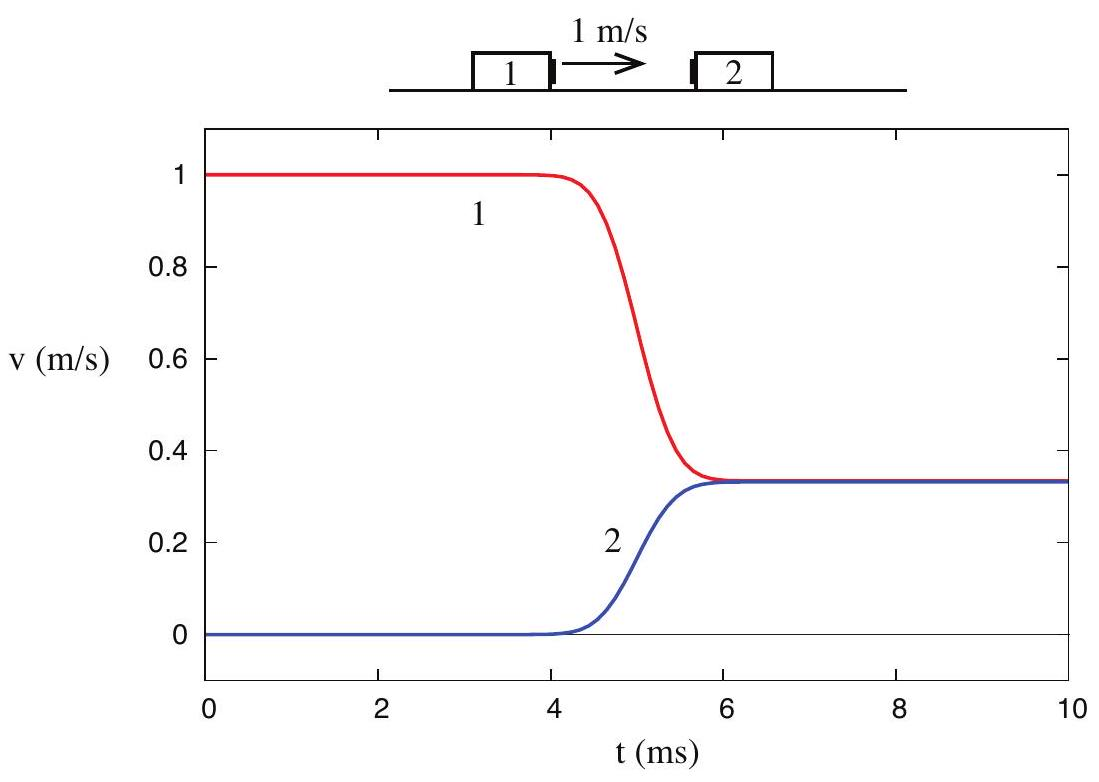
\includegraphics[max width=\textwidth]{2024_09_14_9969b06773f10b6936e8g-072}
\end{center}

Figure 3.3: What would happen if the objects in Figure 1 became stuck together when they collided.

\subsection*{3.1.2 Inertial mass: definition and properties}
At this point, it would seem reasonable to assume that this ratio, $\Delta v_{2} / \Delta v_{1}$, is, in fact, telling us something about an intrinsic property of the two objects, what we have called above their "relative inertia." It is easy, then, to see how one could assign a value to the inertia of any object (at least, conceptually): choose a "standard" object, and decide, arbitrarily, that its inertia will have the numerical value of 1 , in whichever units you choose for it (these units will turn out, in fact, to be kilograms, as you will see in a minute). Then, to determine the inertia of another object, which we will label with the subscript 1 , just arrange a one-dimensional collision between object 1 and the standard, under the right conditions (basically, no net external forces), measure the velocity changes $\Delta v_{1}$ and $\Delta v_{s}$, and take the quantity $-\Delta v_{s} / \Delta v_{1}$ as the numerical value of the ratio of the inertia of object 1 to the inertia of the standard object. In symbols, using the letter $m$ to represent an object's inertia,


\begin{equation*}
\frac{m_{1}}{m_{s}}=-\frac{\Delta v_{s}}{\Delta v_{1}} \tag{3.1}
\end{equation*}


But, since $m_{s}=1$ by definition, this gives us directly the numerical value of $m_{1}$.

The reason we use the letter $m$ is, as you must have guessed, because, in fact, the inertia defined in this way turns out to be identical to what we have traditionally called "mass." More precisely, the quantity defined this way is an object's inertial mass. The remarkable fact, mentioned earlier, that the force of gravity between two objects turns out to be proportional to their inertial masses, allows us to determine the inertial mass of an object by the more traditional procedure of simply weighing it, rather than elaborately staging a collision between it and the standard kilogram on an ice-hockey rink. But, in principle, we could conceive of the existence of two different quantities that should be called "inertial mass" and "gravitational mass," and the identity (or more precisely, the - so far as we know - exact proportionality) of the two is a rather mysterious experimental fact ${ }^{1}$.

In any case, by the way we have constructed it, the inertial mass, defined as in Eq. (3.1), does capture, in a quantitative way, the concept that we were trying to express at the beginning of the chapter: namely, how difficult it may be to set an object in motion. In principle, however, other experiments would need to be conducted to make sure that it does have the properties we have traditionally associated with the concept of mass. For instance, suppose we join together two objects of mass $m$. Is the mass of the resulting object $2 m$ ? Collision experiments would, indeed, show this to be the case with great accuracy in the macroscopic world (with which we are concerned this semester), but this is a good example of how you cannot take anything for granted: at the microscopic level, it is again a fact that the inertial mass of an atomic nucleus is a little less than the sum of the masses of all its constituent protons and neutrons ${ }^{2}$.

Probably the last thing that would need to be checked is that the ratio of inertias is independent

\footnotetext{${ }^{1}$ This fact, elevated to the category of a principle by Einstein (the equivalence principle) is the starting point of the general theory of relativity.\\
${ }^{2}$ And this is not just an unimportant bit of trivia: all of nuclear power depends on this small difference.
}
of the standard. Suppose that we have two objects, to which we have assigned masses $m_{1}$ and $m_{2}$ by arranging for each to collide with the "standard object" independently. If we now arrange for a collision between objects 1 and 2 directly, will we actually find that the ratio of their velocity changes is given by the ratio of the separately determined masses $m_{1}$ and $m_{2}$ ? We certainly would need that to be the case, in order for the concept of inertia to be truly useful; but again, we should not assume anything until we have tested it! Fortunately, the tests would indeed reveal that, in every case, the expected relationship holds ${ }^{3}$\\
\$\$

\begin{equation*}
-\frac{\Delta v_{2}}{\Delta v_{1}}=\frac{m_{1}}{m_{2}} \tag{3.2}
\end{equation*}

\$\$

At this point, we are not just in possession of a useful definition of inertia, but also of a veritable law of nature, as I will explain next.

\subsection*{3.2 Momentum}
For an object of (inertial) mass $m$ moving, in one dimension, with velocity $v$, we define its momentum as


\begin{equation*}
p=m v \tag{3.3}
\end{equation*}


(the choice of the letter $p$ for momentum is apparently related to the Latin word "impetus").\\
We can think of momentum as a sort of extension of the concept of inertia, from an object at rest to an object in motion. When we speak of an object's inertia, we typically think about what it may take to get it moving; when we speak of its momentum, we typically think of that it may take to stop it (or perhaps deflect it). So, both the inertial mass $m$ and the velocity $v$ are involved in the definition.

We may also observe that what looks like inertia in some reference frame may look like momentum in another. For instance, if you are driving in a car towing a trailer behind you, the trailer has only a large amount of inertia, but no momentum, relative to you, because its velocity relative to you is zero; however, the trailer definitely has a large amount of momentum (by virtue of both its inertial mass and its velocity) relative to somebody standing by the side of the road.

\subsection*{3.2.1 Conservation of momentum; isolated systems}
For a system of objects, we treat the momentum as an additive quantity. So, if two colliding objects, of masses $m_{1}$ and $m_{2}$, have initial velocities $v_{1 i}$ and $v_{2 i}$, we say that the total initial momentum of

\footnotetext{${ }^{3}$ Equation 3.2 actually is found to hold also at the microscopic (or quantum) level, although there we prefer to state the result by saying that conservation of momentum holds (see the following section).
}
the system is $p_{i}=m_{1} v_{1 i}+m_{2} v_{2 i}$, and similarly if the final velocities are $v_{1 f}$ and $v_{2 f}$, the total final momentum will be $p_{f}=m_{1} v_{1 f}+m_{2} v_{2 f}$.

We then assert that the total momentum of the system is not changed by the collision. Mathematically, this means


\begin{equation*}
p_{i}=p_{f} \tag{3.4}
\end{equation*}


or


\begin{equation*}
m_{1} v_{1 i}+m_{2} v_{2 i}=m_{1} v_{1 f}+m_{2} v_{2 f} \tag{3.5}
\end{equation*}


But this last equation, in fact, follows directly from Eq. (3.2): to see this, move all the quantities in Eq. (3.5) having to do with object 1 to one side of the equal sign, and those having to do with object 2 to the other side. You then get


\begin{align*}
m_{1}\left(v_{1 i}-v_{1 f}\right) & =m_{2}\left(v_{2 f}-v_{2 i}\right) \\
-m_{1} \Delta v_{1} & =m_{2} \Delta v_{2} \tag{3.6}
\end{align*}


which is just another way to write Equation (3.2). Hence, the result (3.2) ensures the conservation of the total momentum of a system of any two interacting objects ("particles"), regardless of the form the interaction takes, as long as there are no external forces acting on them.

Momentum conservation is one of the most important principles in all of physics, so let me take a little time to explain how we got here and elaborate on this result. First, as I just mentioned, we have been more or less implicitly assuming that the two interacting objects form an isolated system, by which we mean that, throughout, they interact with nothing other than each other. (Equivalently, there are no external forces acting on them.)

It is pretty much impossible to set up a system so that it is really isolated in this strict sense; instead, in practice, we settle for making sure that the external forces on the two objects cancel out. This is what happens on the air tracks with which you will be doing experiments this semester: gravity is acting on the carts, but that force is balanced out by the upwards push of the air from the track. A system on which there is no net external force is as good as isolated for practical purposes, and we will refer to it as such. (It is harder, of course, to completely eliminate friction and drag forces, so we just have to settle for approximately isolated systems in practice.)

Secondly, we have assumed so far that the motion of the two objects is restricted to a straight line one dimension. In fact, momentum is a vector quantity (just like velocity is), so in general we should write

$$
\vec{p}=m \vec{v}
$$

and conservation of momentum, in general, holds as a vector equation for any isolated system in three dimensions:


\begin{equation*}
\vec{p}_{i}=\vec{p}_{f} \tag{3.7}
\end{equation*}


What this means, in turn, is that each separate component $(x, y$ and $z)$ of the momentum will be separately conserved (so Eq. (3.7) is equivalent to three scalar equations, in three dimensions). When we get to study the vector nature of forces, we will see an interesting implication of this, namely, that it is possible for one component of the momentum vector to be conserved, but not another-depending on whether there is or there isn't a net external force in that direction or not. For example, anticipating things a bit, when you throw an object horizontally, as long as you can ignore air drag, there is no horizontal force acting on it, and so that component of the momentum vector is conserved, but the vertical component is changing all the time because of the (vertical) force of gravity.

Thirdly, although this may not be immediately obvious, for an isolated system of two colliding objects the momentum is truly conserved throughout the whole collision process. It is not just a matter of comparing the initial and final velocities: at any of the times shown in Figures 1 through 3 , if we were to measure $v_{1}$ and $v_{2}$ and compute $m_{1} v_{1}+m_{2} v_{2}$, we would obtain the same result. In other words, the total momentum of an isolated system is constant: it has the same value at all times.

Finally, all these examples have involved interactions between only two particles. Can we really generalize this to conclude that the total momentum of an isolated system of any number of particles is constant, even when all the particles may be interacting with each other simultaneously? Here, again, the experimental evidence is overwhelmingly in favor of this hypothesis ${ }^{4}$, but much of our confidence on its validity comes in fact from a consideration of the nature of the internal interactions themselves. It is a mathematical fact that all of the interactions so far known to physics have the property of conserving momentum, whether acting individually or simultaneously. No experiments have ever suggested the existence of an interaction that does not have this property.

\subsection*{3.3 Extended systems and center of mass}
Consider a collection of particles with masses $m_{1}, m_{2}, \ldots$, and located, at some given instant, at positions $x_{1}, x_{2} \ldots$. (We are still, for the time being, considering only motion in one dimension, but all these results generalize easily to three dimensions.) The center of mass of such a system is a mathematical point whose position coordinate is given by


\begin{equation*}
x_{c m}=\frac{m_{1} x_{1}+m_{2} x_{2}+\ldots}{m_{1}+m_{2}+\ldots} \tag{3.8}
\end{equation*}


Clearly, the denominator of (3.8) is just the total mass of the system, which we may just denote by $M$. If all the particles have the same mass, the center of mass will be somehow "in the middle"

\footnotetext{${ }^{4}$ For an important piece of indirect evidence, just consider that any extended object is in reality a collection of interacting particles, and the experiments establishing conservation of momentum almost always involve such extended objects. See the following section for further thoughts on this matter.
}
of all of them; otherwise, it will tend to be closer to the more massive particle(s). The "particles" in question could be spread apart, or they could literally be the "parts" into which we choose to subdivide, for computational purposes, a single extended object.

If the particles are in motion, the position of the center of mass, $x_{c m}$, will in general change with time. For a solid object, where all the parts are moving together, the displacement of the center of mass will just be the same as the displacement of any part of the object. In the most general case, we will have (by subtracting $x_{c m i}$ from $x_{c m f}$ )


\begin{equation*}
\Delta x_{c m}=\frac{1}{M}\left(m_{1} \Delta x_{1}+m_{2} \Delta x_{2}+\ldots\right) \tag{3.9}
\end{equation*}


Dividing Eq. (3.9) by $\Delta t$ and taking the limit as $\Delta t \rightarrow 0$, we get the instantaneous velocity of the center of mass:


\begin{equation*}
v_{c m}=\frac{1}{M}\left(m_{1} v_{1}+m_{2} v_{2}+\ldots\right) \tag{3.10}
\end{equation*}


But this is just


\begin{equation*}
v_{c m}=\frac{p_{s y s}}{M} \tag{3.11}
\end{equation*}


where $p_{\text {sys }}=m_{1} v_{1}+m_{2} v_{2}+\ldots$ is the total momentum of the system.

\subsection*{3.3.1 Center of mass motion for an isolated system}
Equation (3.11) is a very interesting result. Since the total momentum of an isolated system is constant, it tells us that the center of mass of an isolated system of particles moves at constant velocity, regardless of the relative motion of the particles themselves or their possible interactions with each other. As indicated above, this generalizes straightforwardly to more than one dimension, so we can write $\vec{v}_{c m}=\vec{p}_{s y s} / M$. Thus, we can say that, for an isolated system in space, not only the speed, but also the direction of motion of its center of mass does not change with time.

Clearly this result is a sort of generalization of the law of inertia. For a solid, extended object, it does, in fact, provide us with the precise form that the law of inertia must take: in the absence of external forces, the center of mass will just move on a straight line with constant velocity, whereas the object itself may be moving in any way that does not affect the center of mass trajectory. Specifically, the most general motion of an isolated rigid body is a straight line motion of its center of mass at constant speed, combined with a possible rotation of the object as a whole around the center of mass.

For a system that consists of separate parts, on the other hand, the center of mass is generally just a point in space, which may or may not coincide at any time with the position of any of the parts, but which will nonetheless move at constant velocity as long as the system is isolated. This is illustrated by Figure 3.4, where the position vs. time curves have been drawn for the colliding\\
objects of Figure 3.1. I have assumed that object 1 starts out at $x_{1 i}=-5 \mathrm{~mm}$ at $t=0$, and object 2 starts at $x_{2 i}=0$ at $t=0$. Because object 2 has twice the inertia of object 1 , the position of the center of mass, as given by Eq. (3.8), will always be

$$
x_{c m}=x_{1} / 3+2 x_{2} / 3
$$

that is to say, the center of mass will always be in between objects 1 and 2, and its distance from object 2 will always be half its distance to object 1 :

$$
\begin{gathered}
\left|x_{c m}-x_{1}\right|=\frac{2}{3}\left|x_{1}-x_{2}\right| \\
\left|x_{c m}-x_{2}\right|=\frac{1}{3}\left|x_{1}-x_{2}\right|
\end{gathered}
$$

Figure 4 shows that this simple prescription does result in motion with constant velocity for the center of mass (the green straight line), even though the $x$-vs- $t$ curves of the two objects themselves look relatively complicated. (Please check it out! Take a ruler to Fig. 3.4 and verify that the center of mass is, at every instant, where it is supposed to be.)

\begin{center}
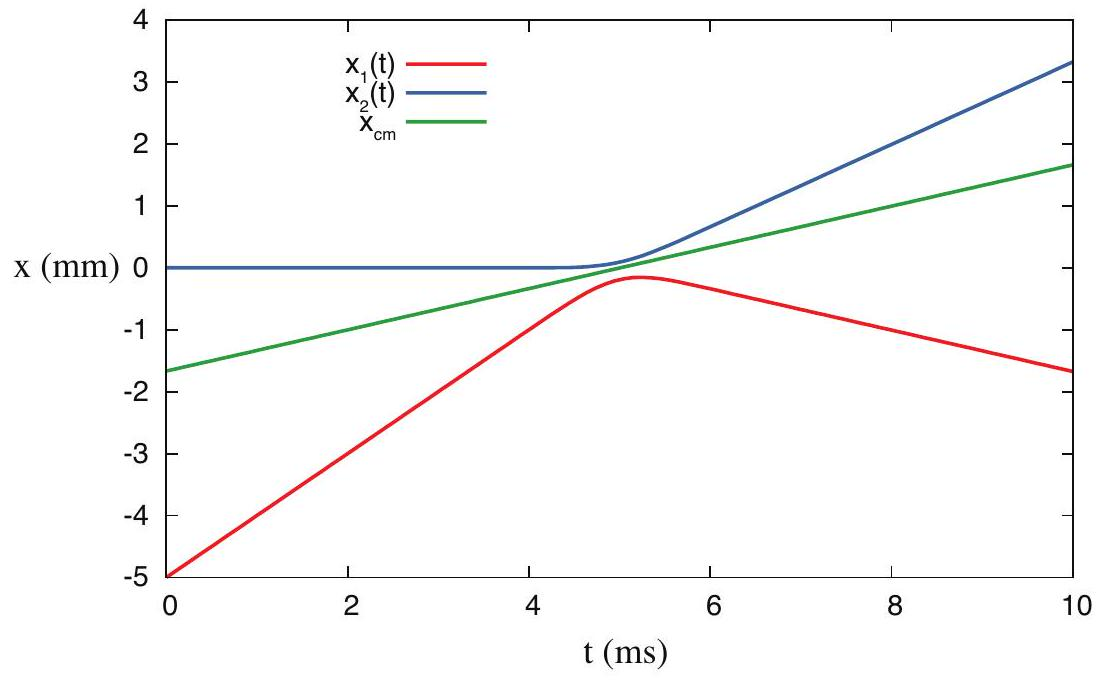
\includegraphics[max width=\textwidth]{2024_09_14_9969b06773f10b6936e8g-078}
\end{center}

Figure 3.4: Position vs. time graph for the objects colliding in Figure 1. The green line shows the position of the center of mass as a function of time.

The concept of center of mass gives us an important way to simplify the description of the motion of potentially complicated systems. We will make good use of it in forthcoming chapters.

A very nice demonstration of the motion of the center of mass in two-body one-dimensional collisions can be found at\\
\href{https://phet.colorado.edu/sims/collision-lab/collision-lab_en.html}{https://phet.colorado.edu/sims/collision-lab/collision-lab\_en.html}\\
(you need to check the "center of mass" box to see it).

\subsection*{3.3.2 Recoil and rocket propulsion}
As we have just seen, you cannot alter the motion of your center of mass without relying on some external force - which is to say, some kind of external support. This is actually something you may have experienced when you are resting on a very slippery surface and you just cannot "get a grip" on it. There is, however, one way to circumvent this problem which, in fact, relies on conservation of momentum itself: if you are carrying something with you, and can throw it away from you at high speed, you will recoil as a result of that. If you can keep throwing things, you (with your store of as yet unthrown things) will speed up a little more every time. This is, in essence, the principle behind rocket propulsion.

Mathematically, consider two objects, of masses $m_{1}$ and $m_{2}$, initially at rest, so their total momentum is zero. If mass 1 is thrown away from mass 2 with a speed $v_{1 f}$, then, by conservation of momentum (always assuming the system is isolated) we must have


\begin{equation*}
0=m_{1} v_{1 f}+m_{2} v_{2 f} \tag{3.12}
\end{equation*}


and therefore $v_{2 f}=-m_{1} v_{1 f} / m_{2}$. This is how a rocket moves forward, by constantly expelling mass (the hot exhaust gas) backwards at a high velocity. Note that, even though both objects move, the center of mass of the whole system does not (in the absence of any external force), as discussed above.

\subsection*{3.4 In summary}
\begin{enumerate}
  \item The inertia of an object is a measure of its tendency to resist changes in its motion. It is quantified by the inertial mass (measured in kilograms).
  \item A system of objects is called isolated (for practical purposes) when there are no net (or unbalanced) external forces acting on any of the objects (the objects may still interact with each other).
  \item When two objects forming an isolated system collide in one dimension, the changes in their velocities are inversely proportional to their inertial masses:
\end{enumerate}

$$
\frac{\Delta v_{1}}{\Delta v_{2}}=-\frac{m_{2}}{m_{1}}
$$

This may be used, in principle, as a way to define the inertial mass operationally.\\
4. The inertial mass thus defined turns out to be exactly (as far as we know) proportional to the object's gravitational mass, which determines the gravitational force of attraction between it and any other object. For this reason, most often we measure an object's inertial mass simply by weighing it.\\
5. The momentum of an object of inertial mass $m$ moving with a velocity $\vec{v}$ is defined as $\vec{p}=m \vec{v}$. The total momentum of a system of objects is defined as the (vector) sum of all the individual momenta.\\
6. (Conservation of momentum) The momentum of an isolated system remains always constant, regardless of how the parts that make up the system may interact with one another.\\
7. In one dimension, the center of mass of a system of particles is a mathematical point whose $x$ coordinate is given by Equation (3.8) above. (In more dimensions, just change the $x$ 's in Eq. (3.8) to $y$ and $z$ to get $y_{c m}$ and $z_{c m}$.)\\
8. The center of mass of a system always moves with a velocity

$$
\vec{v}_{c m}=\frac{\vec{p}_{\text {sys }}}{M}
$$

where $\vec{p}_{\text {sys }}$ is the total momentum of the system, and $M$ its total mass.\\
9. It follows from 8 and 6 above that for an isolated system, the center of mass must always be at rest or moving with constant velocity. This result generalizes the law of inertia to extended objects, or systems of particles.

\subsection*{3.5 Examples}
\subsection*{3.5.1 Reading a collision graph}
The graph shows a collision between two carts (possibly equipped with magnets so that they repel each other before they actually touch) on an air track. The inertia (mass) of cart 1 is 1 kg . Note: this is a position vs. time graph!\\
(a) What are the initial velocities of the carts?\\
(b) What are the final velocities of the carts?\\
(c) What is the mass of the second cart?\\
(d) Does the air track appear to be level? Why? (Hint: does the graph show any evidence of acceleration, for either cart, outside of the collision region?)\\
(e) At the collision time, is the acceleration of the first cart positive or negative? How about the second cart? (Justify your answers.)\\
(f) For the system consisting of the two carts, what is its initial (total) momentum? What is its final momentum?\\
(g) Imagine now that one of the magnets is reversed, so when the carts collide they stick to each other. What would then be the final momentum of the system? What would be its final velocity?

\begin{center}
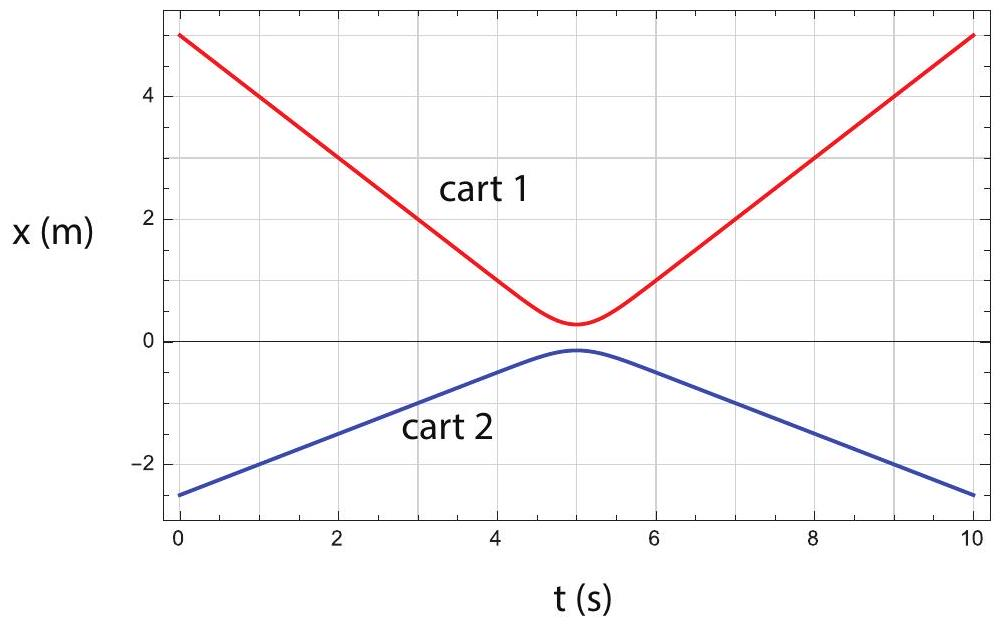
\includegraphics[max width=\textwidth]{2024_09_14_9969b06773f10b6936e8g-081}
\end{center}

Figure 3.5: A collision between two carts.

\section*{Solution}
(a) All the velocities are to be calculated by picking an easy straight part of each curve and calculating

$$
v=\frac{\Delta x}{\Delta t}
$$

for suitable intervals. In this way one gets

$$
\begin{aligned}
& v_{1 i}=-1 \frac{\mathrm{m}}{\mathrm{s}} \\
& v_{2 i}=0.5 \frac{\mathrm{m}}{\mathrm{s}}
\end{aligned}
$$

(b) Similarly, one gets

$$
\begin{aligned}
& v_{1 f}=1 \frac{\mathrm{m}}{\mathrm{s}} \\
& v_{2 f}=-0.5 \frac{\mathrm{m}}{\mathrm{s}}
\end{aligned}
$$

(c) Use this equation, or equivalent (conservation of momentum is OK)

$$
\begin{gathered}
\frac{m_{2}}{m_{1}}=-\frac{\Delta v_{1}}{\Delta v_{2}} \\
\frac{m_{2}}{m_{1}}=-\frac{1-(-1)}{-0.5-0.5}=2
\end{gathered}
$$

so the mass of the second cart is 2 kg .\\
(d) Yes, the track appears to be level because the carts do not show any evidence of acceleration outside of the collision region (the position vs. time curves are straight lines outside of the region approximately given by $4.5 \mathrm{~s}<t<5.5 \mathrm{~s}$ ).\\
(e) The acceleration of the first cart is positive. You can see this either graphically (the curve is like a parabola that opens upwards, i.e., concave), or algebraically (the cart's velocity increases, going from $-1 \mathrm{~m} / \mathrm{s}$ to $1 \mathrm{~m} / \mathrm{s}$ )\\
Similarly, the acceleration of the second cart is negative. The curve is like a parabola that opens downwards, i.e., convex; or, algebraically, the cart's velocity decreases, going from $0.5 \mathrm{~m} / \mathrm{s}$ to $-0.5 \mathrm{~m} / \mathrm{s}$.\\
(f) The initial momentum of the system is

$$
p_{i}=m_{1} v_{1 i}+m_{2} v_{2 i}=(1 \mathrm{~kg}) \times\left(-1 \frac{\mathrm{m}}{\mathrm{s}}\right)+(2 \mathrm{~kg}) \times\left(0.5 \frac{\mathrm{m}}{\mathrm{s}}\right)=0
$$

The final momentum is

$$
p_{f}=m_{1} v_{1 f}+m_{2} v_{2 f}=(1 \mathrm{~kg}) \times\left(1 \frac{\mathrm{m}}{\mathrm{s}}\right)+(2 \mathrm{~kg}) \times\left(-0.5 \frac{\mathrm{m}}{\mathrm{s}}\right)=0
$$

You could also just say that the final momentum should be the same as the initial momentum, since the system appears to be isolated.\\
(g) The momentum should be conserved in this case as well, so $p_{f}=0$. The velocity would be

$$
v_{f}=\frac{p_{f}}{m_{1}+m_{2}}=0
$$

\subsection*{3.5.2 Collision in different reference frames, center of mass, and recoil}
An $80-\mathrm{kg}$ hockey player (call him player 1), moving at $3 \mathrm{~m} / \mathrm{s}$ to the right, collides with a $90-\mathrm{kg}$ player (player 2) who was moving at $2 \mathrm{~m} / \mathrm{s}$ to the left. For a brief moment, they are stuck sliding together as they grab at each other.\\
(a) What is their joint velocity as they slide together?\\
(b) What was the velocity of their center of mass before and after the collision?\\
(c) What does the collision look like to another player that was skating initially at $1.5 \mathrm{~m} / \mathrm{s}$ to the right? Give all the initial and final velocities as seen by this player, and show explicitly that momentum is also conserved in this player's frame of reference.\\
(d) Eventually, the $90-\mathrm{kg}$ player manages to push the other one back, in such a way that player 1 (the $80-\mathrm{kg}$ player) ends up moving at $1 \mathrm{~m} / \mathrm{s}$ to the left relative to player 2. What are their final velocities in the earth frame of reference?

\section*{Solution}
(a) Call the initial velocities $v_{1 i}$ and $v_{2 i}$, the joint final velocity $v_{f}$, and assume the two players are an isolated system for practical purposes. Then conservation of momentum reads


\begin{equation*}
m_{1} v_{1 i}+m_{2} v_{2 i}=\left(m_{1}+m_{2}\right) v_{f} \tag{3.13}
\end{equation*}


Solving for the final velocity, we get


\begin{equation*}
v_{f}=\frac{m_{1} v_{1 i}+m_{2} v_{2 i}}{m_{1}+m_{2}} \tag{3.14}
\end{equation*}


Substituting the values given, we get


\begin{equation*}
v_{f}=\frac{80 \times 3-90 \times 2}{170}=0.353 \frac{\mathrm{m}}{\mathrm{s}} \tag{3.15}
\end{equation*}


(b) According to Eq. (3.10), the velocity of the center of mass, $v_{c m}$, is just the same as what we just calculated (Eq. (3.14) above). This makes sense: after the collision, if the players are moving together, their system's center of mass has to be moving with them. Also, if the system is isolated, the center of mass velocity should be the same before and after the collision. So the answer is $v_{c m}=v_{f}=0.353 \mathrm{~m} / \mathrm{s}$\\
(c) Let me refer to this third player as "player 3," and introduce a subscript " 3 " to refer to the quantities as seen in his frame of reference. Let also the subscript " $E$ " denote the original, "Earth" reference frame. From Eq. (1.19), we have then (for player 1, for instance)


\begin{equation*}
v_{31}=v_{3 E}+v_{E 1}=v_{E 1}-v_{E 3} \tag{3.16}
\end{equation*}


because $v_{3 E}$, the "velocity of the Earth in player 3 's reference frame," is clearly equal to $-v_{E 3}$, the negative of the velocity of player 3 relative to the Earth. Basically, what Eq. (3.16) is saying is\\
that to convert all the Earth-frame velocities to the reference frame of player 3, we just need to subtract $1.5 \mathrm{~m} / \mathrm{s}$ from them. This gives us


\begin{align*}
v_{31, i} & =3 \frac{\mathrm{m}}{\mathrm{s}}-1.5 \frac{\mathrm{m}}{\mathrm{s}}=1.5 \frac{\mathrm{m}}{\mathrm{s}} \\
v_{32, i} & =-2 \frac{\mathrm{m}}{\mathrm{s}}-1.5 \frac{\mathrm{m}}{\mathrm{s}}=-3.5 \frac{\mathrm{m}}{\mathrm{s}} \\
v_{31, f}=v_{32, f} & =0.353 \frac{\mathrm{m}}{\mathrm{s}}-1.5 \frac{\mathrm{m}}{\mathrm{s}}=-1.147 \frac{\mathrm{m}}{\mathrm{s}} \tag{3.17}
\end{align*}


The total initial momentum in player's 3 reference frame is then


\begin{equation*}
p_{s y s, i}=m_{1} v_{31, i}+m_{2} v_{32, i}=80 \times 1.5+90 \times(-3.5)=-195 \frac{\mathrm{kg} \cdot \mathrm{m}}{\mathrm{s}} \tag{3.18}
\end{equation*}


and the final momentum is


\begin{equation*}
p_{s y s, f}=\left(m_{1}+m_{2}\right) v_{31, f}=170 \times(-1.147)=-195 \frac{\mathrm{kg} \cdot \mathrm{m}}{\mathrm{s}} \tag{3.19}
\end{equation*}


So the total momentum is conserved in player 3's reference frame. The reason for this is that this is an inertial reference frame, because the velocity of player 3 does not change.\\
(d) For this part of the problem, we are back to the original reference frame (the Earth reference frame), and we can drop the " $E$ " subscript. For this new process, the final velocities from part (a) become the initial velocities, so we have $v_{1 i}=v_{2 i}=0.353 \mathrm{~m} / \mathrm{s}$. [Note: alternatively, since the system is isolated throughout, it would be OK in this case to use the velocities before the collision to calculate its total momentum, which also needs to be conserved in this process.] We are also told that the final velocity of player 1 relative to player 2 is $v_{21, f}=v_{1 f}-v_{2 f}=-1 \mathrm{~m} / \mathrm{s}$. So we have two equations to solve:


\begin{align*}
\left(m_{1}+m_{2}\right) \times\left(0.353 \frac{\mathrm{m}}{\mathrm{s}}\right) & =m_{1} v_{1 f}+m_{2} v_{2 f} \quad \text { (conservation of momentum) } \\
v_{1 f}-v_{2 f} & =-1 \frac{\mathrm{m}}{\mathrm{s}} \quad \text { (final relative velocity) } \tag{3.20}
\end{align*}


Leaving aside the units for the moment, to make the equations more readable (the final units will work out, if we make sure to use SI units all along), we have:


\begin{align*}
(80+90) \times 0.353 & =80 v_{1 f}+90 v_{2 f} \\
v_{1 f} & =v_{2 f}-1 \tag{3.21}
\end{align*}


Now substitute the second equation, which I have "solved" already for $v_{1 f}$, in the first equation and solve for $v_{2 f}$. The result is $v_{2 f}=0.824 \mathrm{~m} / \mathrm{s}$, which, when substituted back in the relative velocity equation, gives $v_{1 f}=-0.176 \mathrm{~m} / \mathrm{s}$.

\subsection*{3.6 Problems}
\section*{Problem 1}
This figure shows the position vs. time graph for two objects before and after they collide. Assume that they form an isolated system.\\
(a) What are the velocities of the two objects before and after the collision? (Hint: you will get a more accurate result if you choose the initial and final times where the lines go exactly through a point on the grid shown.)\\
(b) Given the result in (a), what is the ratio of the inertias of the two objects?

\begin{center}
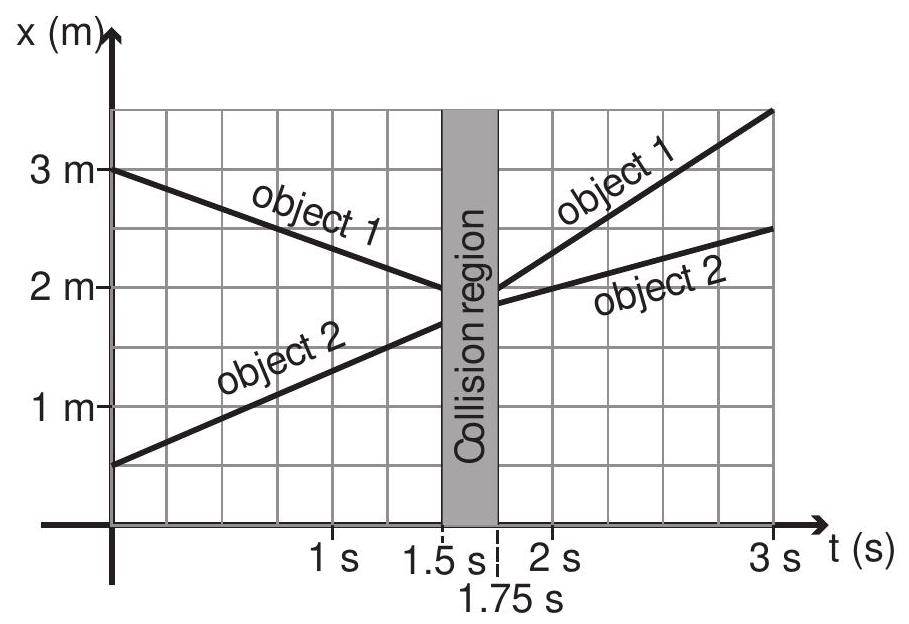
\includegraphics[max width=\textwidth]{2024_09_14_9969b06773f10b6936e8g-085}
\end{center}

\section*{Problem 2}
A car and a truck collide on a very slippery highway. The car, with a mass of 1600 kg , was initially moving at 50 mph . The truck, with a mass of 3000 kg , hit the car from behind at 65 mph . Assume the two vehicles form an isolated system in what follows.\\
(a) If, immediately after the collision, the vehicles separate and the truck's velocity is found to be 55 mph in the same direction it was going, how fast (in miles per hour) is the car moving?\\
(b) If instead the vehicles end up stuck together, what will be their common velocity immediately after the collision?

\section*{Problem 3}
A $4-\mathrm{kg}$ gun fires a $0.012-\mathrm{kg}$ bullet at a $3-\mathrm{kg}$ block of wood that is initially at rest. The bullet is embedded in the block, and they move together, immediately after the impact, with a velocity of $3.5 \mathrm{~m} / \mathrm{s}$.\\
(a) What was the velocity of the bullet just before impact?\\
(b) In order to shoot a bullet at this speed, what must have been the recoil speed of the gun?

\section*{Problem 4}
A 2-kg object, moving at $1 \mathrm{~m} / \mathrm{s}$, collides with a $1-\mathrm{kg}$ object that is initially at rest. After the collision, the two objects are found to move away from each other at $1 \mathrm{~m} / \mathrm{s}$. Assume they form an isolated system.\\
(a) What are their actual final velocities in the Earth reference frame?\\
(b) What is the velocity of the center of mass of this system? Does it change as a result of the collision?

\section*{Problem 5}
Imagine you are stranded on a frozen lake (that means no friction-no traction!), with just a bow and a quiver of arrows. Each arrow has a mass of 0.02 kg , and with your bow can shoot them at a speed of $90 \mathrm{~m} / \mathrm{s}$ (relative to you-but you might as well assume that this is the arrow's velocity relative to the earth, since, as you will see, your recoil velocity will end up being pretty small anyway). So you decide to use them to propel yourself back to shore.\\
(a) Suppose your mass (plus the bow and arrows) is 70 kg . When you shoot an arrow, starting from rest, with what speed do you recoil?\\
(b) Suppose you try to be really clever, and tie a string to the arrow, with the other end of the string tied around your waist. The idea is to get the arrow to pull you forward. Will this work? (Hint: remember part (a). What will happen when the string becomes taut?)

\section*{Problem 6}
An object's position function is given by $x_{1}(t)=5+10 t$ (with $x_{1}$ in meters if $t$ is in seconds). A second object's position function is $x_{2}(t)=5-6 t$.\\
(a) If the first object's mass is $1 / 3$ the mass of the second one, what is the position of the system's center of mass as a function of time?\\
(b) Under the same assumption, what is the velocity of the system's center of mass?

\section*{Chapter 4}
\section*{Kinetic Energy}
\subsection*{4.1 Kinetic Energy}
For a long time in the development of classical mechanics, physicists were aware of the existence of two different quantities that one could define for an object of inertia $m$ and velocity $v$. One was the momentum, $m v$, and the other was something proportional to $m v^{2}$. Despite their obvious similarities, these two quantities exhibited different properties and seemed to be capturing different aspects of motion.

When things got finally sorted out, in the second half of the 19th century, the quantity $\frac{1}{2} m v^{2}$ came to be recognized as a form of energy - itself perhaps the most important concept in all of physics. Kinetic energy, as this quantity is called, may be the most obvious and intuitively understandable kind of energy, and so it is a good place to start our study of the subject.

We will use the letter $K$ to denote kinetic energy, and, since it is a form of energy, we will express it in the units especially named for this purpose, which is to say joules (J). 1 joule is $1 \mathrm{~kg} \cdot \mathrm{m}^{2} / \mathrm{s}^{2}$. In the definition


\begin{equation*}
K=\frac{1}{2} m v^{2} \tag{4.1}
\end{equation*}


the letter $v$ is meant to represent the magnitude of the velocity vector, that is to say, the speed of the particle. Hence, unlike momentum, kinetic energy is not a vector, but a scalar: there is no sense of direction associated with it. In three dimensions, one could write


\begin{equation*}
K=\frac{1}{2} m\left(v_{x}^{2}+v_{y}^{2}+v_{z}^{2}\right) \tag{4.2}
\end{equation*}


There is, therefore, some amount of kinetic energy associated with each component of the velocity vector, but in the end they are all added together in a lump sum.

For a system of particles, we will treat kinetic energy as an additive quantity, just like we did for momentum, so the total kinetic energy of a system will just be the sum of the kinetic energies of all the particles making up the system. Note that, unlike momentum, this is a scalar (not a vector) sum, and most importantly, that kinetic energy is, by definition, always positive, so there can be no question of a "cancellation" of one particle's kinetic energy by another, again unlike what happened with momentum. Two objects of equal mass moving with equal speeds in opposite directions have a total momentum of zero, but their total kinetic energy is definitely nonzero. Basically, the kinetic energy of a system can never be zero as long as there is any kind of motion going on in the system.

\subsection*{4.1.1 Kinetic energy in collisions}
To gain some further insights into the concept of kinetic energy, and the ways in which it is different from momentum, it is useful to look at it in the same setting in which we "discovered" momentum, namely, one-dimensional collisions in an isolated system. If we look again at the collision represented in Figure 1 of Chapter 3, reproduced below,

\begin{center}
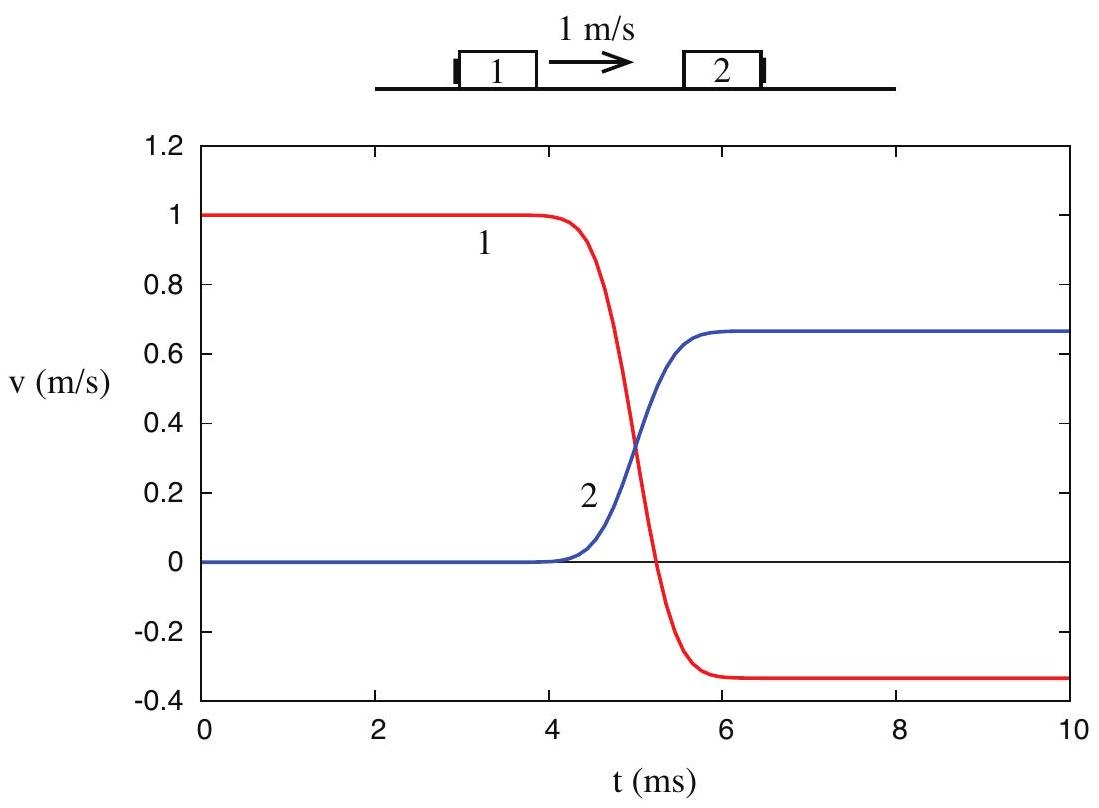
\includegraphics[max width=\textwidth]{2024_09_14_9969b06773f10b6936e8g-088}
\end{center}

Figure 4.1: Elastic collision in an isolated system. (Figure 3.1.)\\
we can use the definition (4.1) to calculate the initial and final values of $K$ for each object, and for the system as a whole. Remember we found that, for this particular system, $m_{2}=2 m_{1}$, so we can just set $m_{1}=1 \mathrm{~kg}$ and $m_{2}=2 \mathrm{~kg}$, for simplicity. The initial and final velocities are $v_{1 i}=1 \mathrm{~m} / \mathrm{s}$,\\
$v_{2 i}=0, v_{1 f}=-1 / 3 \mathrm{~m} / \mathrm{s}, v_{2 f}=2 / 3 \mathrm{~m} / \mathrm{s}$, and so the kinetic energies are

$$
K_{1 i}=\frac{1}{2} \mathrm{~J}, K_{2 i}=0 ; \quad K_{1 f}=\frac{1}{18} \mathrm{~J}, K_{2 f}=\frac{4}{9} \mathrm{~J}
$$

Note that $1 / 18+4 / 9=9 / 18=1 / 2$, and so

$$
K_{s y s, i}=K_{1 i}+K_{2 i}=\frac{1}{2} \mathrm{~J}=K_{1 f}+K_{2 f}=K_{s y s, f}
$$

In words, we find that, in this collision, the final value of the total kinetic energy is the same as its initial value, and so it looks like we have "discovered" another conserved quantity (besides momentum) for this system.

This belief may be reinforced if we look next at the collision depicted in Figure 2 of Chapter 3, again reproduced below. Recall I pointed out back then that we can think of this as being really the same collision as depicted in Figure 3.1, only looked at from another frame of reference (one moving initially to the right at $1 \mathrm{~m} / \mathrm{s}$ ). We will have more to say about how to transform quantities from a frame of reference to another by the end of the chapter.

\begin{center}
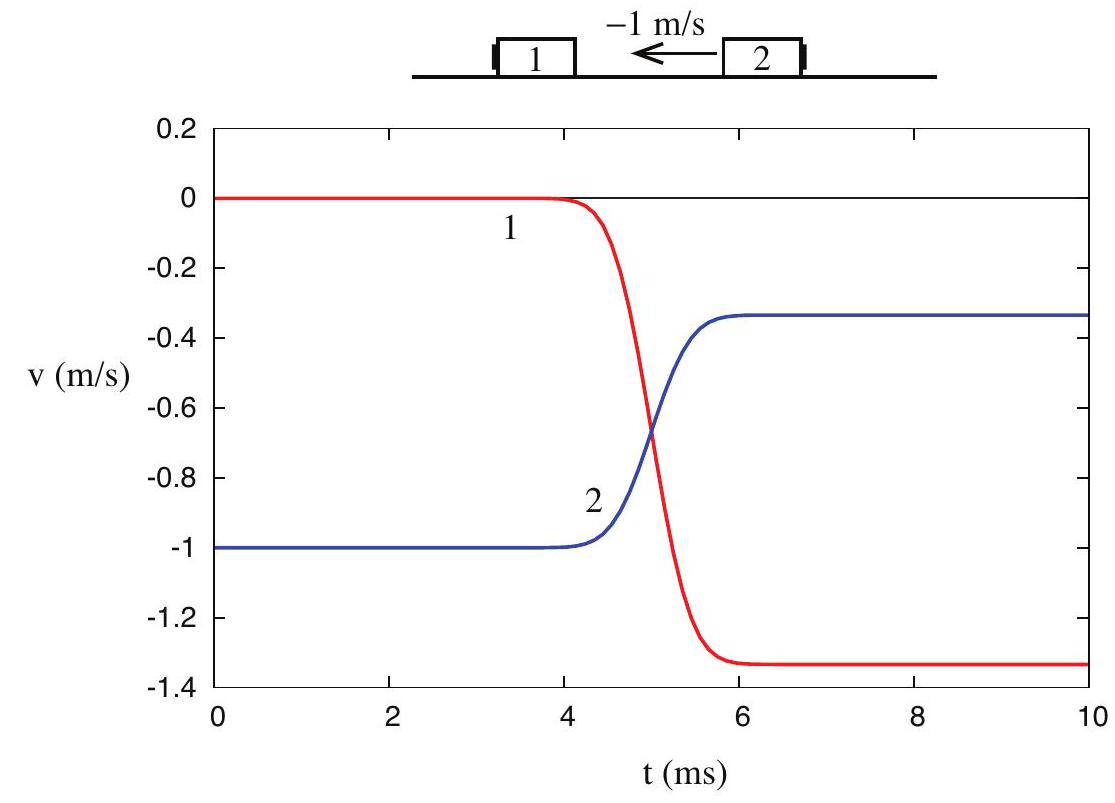
\includegraphics[max width=\textwidth]{2024_09_14_9969b06773f10b6936e8g-089}
\end{center}

Figure 4.2: Another elastic collision, equivalent to the one in Figure 1 as seen from another reference frame. (Figure 3.2.)

In any case, as observed there, all we need to do is add $-1 \mathrm{~m} / \mathrm{s}$ to all the velocities in the previous problem, so we have $v_{1 i}=0, v_{2 i}=-1 \mathrm{~m} / \mathrm{s}, v_{1 f}=-4 / 3 \mathrm{~m} / \mathrm{s}, v_{2 f}=-1 / 3 \mathrm{~m} / \mathrm{s}$. The corresponding kinetic energies are, accordingly, $K_{1 i}=0, K_{2 i}=1 \mathrm{~J}, K_{1 f}=\frac{8}{9} \mathrm{~J}, K_{2 f}=\frac{1}{9} \mathrm{~J}$. These are all different\\
from the values we had in the previous example, but note that once again the total kinetic energy after the collision equals the total kinetic energy before-namely, 1 J in this case ${ }^{1}$.

Things are, however, very different when we consider the third collision example shown in Chapter 3 , namely, the one where the two objects are stuck together after the collision.

\begin{center}
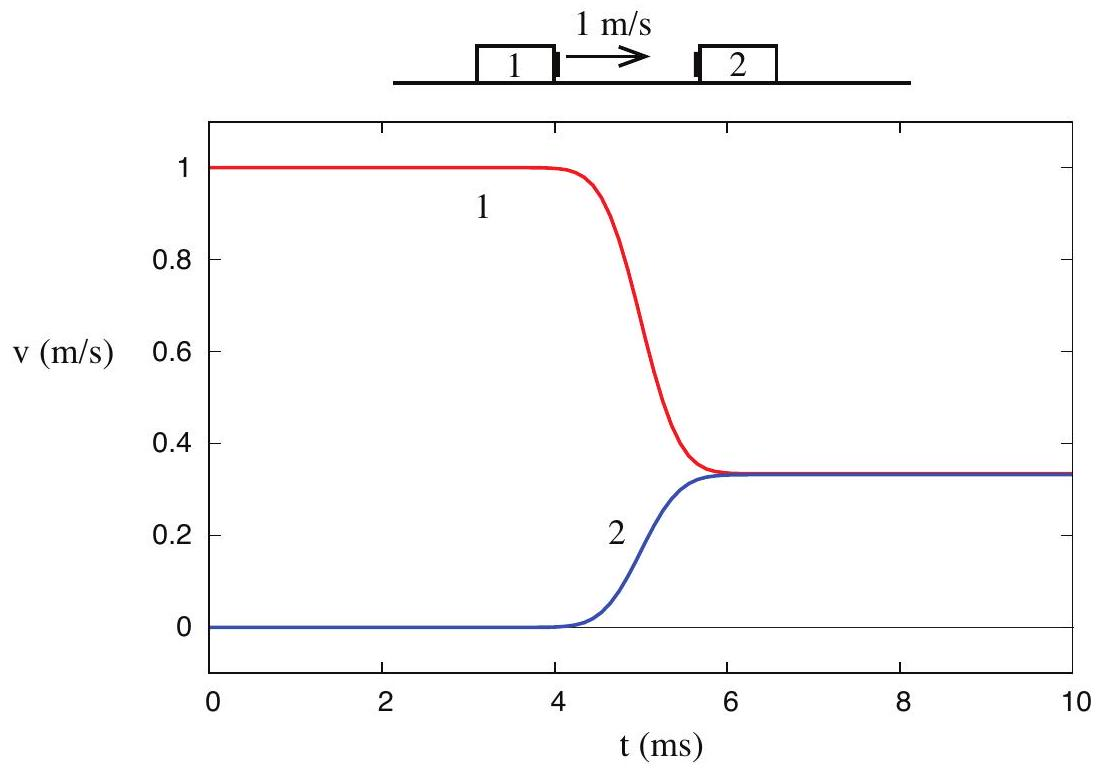
\includegraphics[max width=\textwidth]{2024_09_14_9969b06773f10b6936e8g-090}
\end{center}

Figure 4.3: A totally inelastic collision. (Figure 3.3.)

Their joint final velocity, consistent with conservation of momentum, is $v_{1 f}=v_{2 f}=1 / 3 \mathrm{~m} / \mathrm{s}$. Since the system starts as in Figure 4.1, its kinetic energy is initially $K_{\text {sys }, i}=\frac{1}{2} \mathrm{~J}$, but after the collision we have only

$$
K_{\text {sys }, f}=\frac{1}{2}(3 \mathrm{~kg})\left(\frac{1}{3} \frac{\mathrm{m}}{\mathrm{s}}\right)^{2}=\frac{1}{6} \mathrm{~J}
$$

So kinetic energy is not conserved in this case at all.\\
What this shows, however, is that unlike the total momentum of a system, which is completely unaffected by internal interactions, the total kinetic energy does depend on the details of the interaction, and thus conveys some information about its nature. We can then refine our study of collisions to distinguish two kinds: the ones where the initial kinetic energy is recovered after the collision, which we will call elastic, and the ones where it is not, which we call inelastic. A

\footnotetext{${ }^{1}$ This is, of course, consistent with the principle of relativity I told you about in Chapter 2: if the process in Fig. 4.2 is really the same as the one in Fig. 4.1, only viewed in a different inertial reference frame, then, if energy is seen to be conserved in one frame, it should also be seen to be conserved in the other. More on this below, in Section 4.2.1.
}
special case of inelastic collision is the one called totally inelastic, where the two objects end up stuck together, as in Figure 4.3. As we shall see later, the kinetic energy "deficit" is largest in that case.

I have said above that in an elastic collision the kinetic energy is "recovered," and I prefer this terminology to "conserved," because, in fact, unlike the total momentum, the total kinetic energy of a system does not remain constant throughout the interaction, not even during an elastic collision. The simplest example to show this would be an elastic, head-on collision between two objects of equal mass, moving at the same speed towards each other. In the course of the collision, both objects are brought momentarily to a halt before they reverse direction and bounce back, and at that instant, the total kinetic energy is zero.

You can also examine Figures 4.1 and 4.2 above, and calculate, from the graphs, the value of the total kinetic energy during the collision. You will see that it dips to a minimum, and then comes back to its initial value (see also Figure 4.5, later in this chapter). Conventionally, we may talk of kinetic energy as being "conserved" in elastic collisions, but it is important to realize that we are looking at a different kind of "conservation" than what we had with the total momentum, which was constant before, during, and after the interaction, as long as the system remained isolated.

Elastic collisions do suggest that, whatever the ultimate nature of this thing we call "energy" might be, it may be possible to store it in some form (in this case, during the course of the collision), and then recover it, as kinetic energy, eventually. This paves the way for the introduction of other kinds of "energy" besides kinetic energy, as we shall see in a later chapter, and the possibility of interconversion to take place among these kinds. For the moment, we shall simply say that in an elastic collision some amount of kinetic energy is temporarily stored as some kind of "internal energy," and after the collision this is converted back into kinetic energy; whereas, in an inelastic collision, some amount of kinetic energy gets irrevocably converted into some "internal energy," and we never get it back.

Since whatever ultimately happens depends on the details and the nature of the interaction, we will be led to distinguish between "conservative" interactions, where kinetic energy is reversibly stored as some other form of energy somewhere, and "dissipative" interactions, where the energy conversion is, at least in part, irreversible. Clearly, elastic collisions are associated with conservative interactions and inelastic collisions are associated with dissipative interactions. This preliminary classification of interactions will have to be reviewed a little more carefully, however, in the next chapter.

\subsection*{4.1.2 Relative velocity and coefficient of restitution}
An interesting property of elastic collisions can be disclosed from a careful study of figures 4.1 and 4.2. In both cases, as you can see, the relative velocity of the two objects colliding has the same magnitude (but opposite sign) before and after the collision. In other words: in an elastic collision, the objects end up moving apart at the same rate as they originally came together.

Recall that, in Chapter 1, we defined the velocity of object 2 relative to object 1 as the quantity


\begin{equation*}
v_{12}=v_{2}-v_{1} \tag{4.3}
\end{equation*}


(compare Eq. (1.21); and similarly the velocity of object 1 relative to object 2 is $v_{21}=v_{1}-v_{2}$. With this definition you can check that, indeed, the collisions shown in Figs. 4.1 and 4.2 satisfy the equality


\begin{equation*}
v_{12, i}=-v_{12, f} \tag{4.4}
\end{equation*}


(note that we could equally well have used $v_{21}$ instead of $v_{12}$ ). For instance, in Fig. 4.1, $v_{12, i}=$ $v_{2 i}-v_{1 i}=-1 \mathrm{~m} / \mathrm{s}$, whereas $v_{12, f}=2 / 3-(-1 / 3)=1 \mathrm{~m} / \mathrm{s}$. So the objects are initially moving towards each other at a rate of 1 m per second, and they end up moving apart just as fast, at 1 m per second. Visually, you should notice that the distance between the red and blue curves is the same before and after (but not during) the collision; the fact that they cross accounts for the difference in sign of the relative velocity, which in turns means simply that before the collision they were coming together, and afterwards they are moving apart.

It takes only a little algebra to show that Eq. (4.4) follows from the joint conditions of conservation of momentum and conservation of kinetic energy. The first one $\left(p_{i}=p_{f}\right)$ clearly has the form


\begin{equation*}
m_{1} v_{1 i}+m_{2} v_{2 i}=m_{1} v_{1 f}+m_{2} v_{2 f} \tag{4.5}
\end{equation*}


whereas the second one $\left(K_{i}=K_{f}\right)$ can be written as


\begin{equation*}
\frac{1}{2} m_{1} v_{1 i}^{2}+\frac{1}{2} m_{2} v_{2 i}^{2}=\frac{1}{2} m_{1} v_{1 f}^{2}+\frac{1}{2} m_{2} v_{2 f}^{2} \tag{4.6}
\end{equation*}


We can cancel out all the factors of $1 / 2$ in Eq. $(4.6)^{2}$, then rearrange it so that quantities belonging to object 1 are on one side, and quantities belonging to object 2 are on the other. We get


\begin{align*}
m_{1}\left(v_{1 i}^{2}-v_{1 f}^{2}\right) & =-m_{2}\left(v_{2 i}^{2}-v_{2 f}^{2}\right) \\
m_{1}\left(v_{1 i}-v_{1 f}\right)\left(v_{1 i}+v_{1 f}\right) & =-m_{2}\left(v_{2 i}-v_{2 f}\right)\left(v_{2 i}+v_{2 f}\right) \tag{4.7}
\end{align*}


(using the fact that $a^{2}-b^{2}=(a+b)(a-b)$ ). Note, however, that Eq. (4.5) can also be rewritten as

$$
m_{1}\left(v_{1 i}-v_{1 f}\right)=-m_{2}\left(v_{2 i}-v_{2 f}\right)
$$

\footnotetext{${ }^{2}$ You may be wondering, just why do we define kinetic energy with a factor $1 / 2$ in front, anyway? There is no good answer at this point. Let's just say it will make the definition of "potential energy" simpler later, particularly as regards its relationship to force.
}This immediately allows us to cancel out the corresponding factors in Eq (4.7), so we are left with $v_{1 i}+v_{1 f}=v_{2 i}+v_{2 f}$, which can be rewritten as


\begin{equation*}
v_{1 f}-v_{2 f}=v_{2 i}-v_{1 i} \tag{4.8}
\end{equation*}


and this is equivalent to (4.4).\\
So, in an elastic collision the speed at which the two objects move apart is the same as the speed at which they came together, whereas, in what is clearly the opposite extreme, in a totally inelastic collision the final relative speed is zero-the objects do not move apart at all after they collide. This suggests that we can quantify how inelastic a collision is by the ratio of the final to the initial magnitude of the relative velocity. This ratio is denoted by $e$ and is called the coefficient of restitution. Formally,


\begin{equation*}
e=-\frac{v_{12, f}}{v_{12, i}}=-\frac{v_{2 f}-v_{1 f}}{v_{2 i}-v_{1 i}} \tag{4.9}
\end{equation*}


For an elastic collision, $e=1$, as required by Eq. (4.4). For a totally inelastic collision, like the one depicted in Fig. 3, $e=0$. For a collision that is inelastic, but not totally inelastic, $e$ will have some value in between these two extremes. This knowledge can be used to "design" inelastic collisions (for homework problems, for instance!): just pick a value for $e$, between 0 and 1, in Eq. (4.9), and combine this equation with the conservation of momentum requirement (4.5). The two equations then allow you to calculate the final velocities for any values of $m_{1}, m_{2}$, and the initial velocities. Figure 4.4 below, for example, shows what the collision in Figure 4.1 would have been like, if the coefficient of restitution had been 0.6 instead of 1 . You can check, by solving (4.5) and (4.9) together, and using the initial velocities, that $v_{1 f}=-1 / 15 \mathrm{~m} / \mathrm{s}=-0.0667 \mathrm{~m} / \mathrm{s}$, and $v_{2 f}=8 / 15 \mathrm{~m} / \mathrm{s}$ $=0.533 \mathrm{~m} / \mathrm{s}$.

\begin{center}
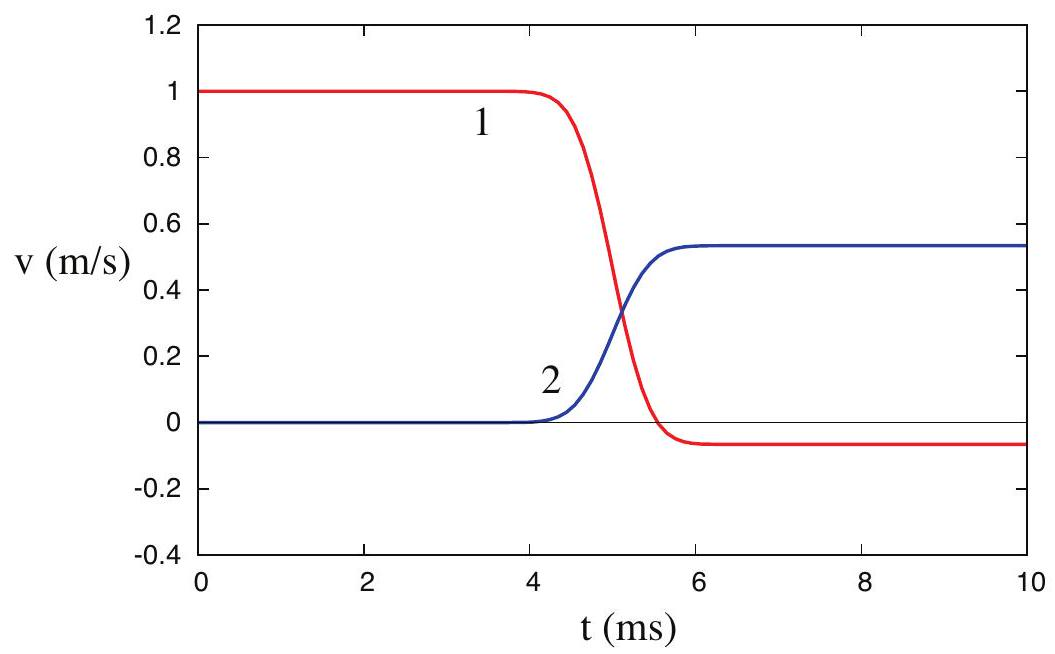
\includegraphics[max width=\textwidth]{2024_09_14_9969b06773f10b6936e8g-093}
\end{center}

Figure 4.4: An $e=0.6$ collision between objects with the same inertias and initial velocities as in Figure 1.

Although, as I just mentioned, for most "normal" collisions the coefficient of restitution will be a positive number between 1 and 0 , there can be exceptions to this. If one of the objects passes through the other (like a bullet through a target, for instance), the value of $e$ will be negative (although still between 0 and 1 in magnitude). And $e$ can be greater than 1 for so-called "explosive collisions," where some amount of extra energy is released, and converted into kinetic energy, as the objects collide. (For instance, two hockey players colliding on the rink and pushing each other away.) In this case, the objects may well fly apart faster than they came together.

An extreme example of a situation with $e>0$ is an explosive separation, which is when the two objects are initially moving together and then fly apart. In that case, the denominator of Eq. (4.9) is zero, and so $e$ is formally infinite. This suggests, what is in fact the case, namely, that although explosive processes are certainly important, describing them through the coefficient of restitution is rare, even when it would be formally possible. In practice, use of the coefficient of restitution is mostly limited to the elastic-to-completely inelastic range, that is, $0 \leq e \leq 1$.

\section*{4.2 "Convertible" and "translational" kinetic energy}
Figure 4.5 shows how the total kinetic energy varies with time, for the two objects shown colliding in Figure 4.1, depending on the details of the collision, namely, on the value of $e$. The three curves shown cover the elastic case, $e=1$ (Figure 4.1), the totally inelastic case, $e=0$ (Figure 4.3), and the inelastic case with $e=0.6$ of Figure 4.4. Recall that the total momentum is conserved in all three cases.

\begin{center}
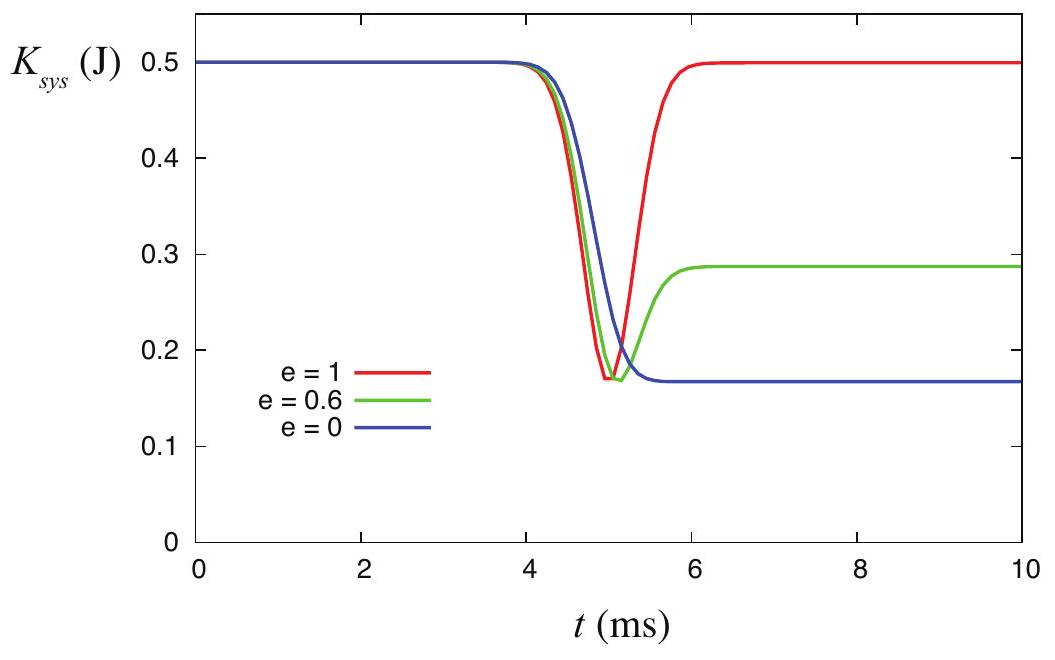
\includegraphics[max width=\textwidth]{2024_09_14_9969b06773f10b6936e8g-094}
\end{center}

Figure 4.5: The total kinetic energy as a function of time for the collisions shown in Figures 1, 3 and 4, respectively.

Figure 4.5 shows that the greatest loss of kinetic energy happens for the totally inelastic collision, which, as we will see in a moment, is, in fact, a general result. That being the case, the figure also shows that it may not be always be possible to bring the total kinetic energy down to zero, even temporarily. The reason for this is that, if momentum is conserved, the velocity of the center of mass cannot change, so if the center of mass was moving before the collision, it must still be moving afterwards; and, as mentioned in this chapter's introduction, as long as there is motion in a system, its total kinetic energy cannot be zero.

All of this suggests that it should be possible to break up a system's total kinetic energy into two parts: one part associated with the motion of the center of mass, which cannot change in any momentum-conserving collision, and one part associated with the relative motion of the parts that make up the system. This second part would vanish irreversibly in a totally inelastic collision, whereas it would recover its original value in an elastic collision.

The way to see this mathematically, for a system of two objects with masses $m_{1}$ and $m_{2}$, is to introduce the center of mass velocity $v_{c m}$ [Eq. (3.10)]

$$
v_{c m}=\frac{m_{1} v_{1}+m_{2} v_{2}}{m_{1}+m_{2}}
$$

and the relative velocity $v_{12}=v_{2}-v_{1}$ (Eq. (4.3) above), and observe that the velocities $v_{1}$ and $v_{2}$ can be written, respectively, as


\begin{align*}
& v_{1}=v_{c m}-\frac{m_{2}}{m_{1}+m_{2}} v_{12} \\
& v_{2}=v_{c m}+\frac{m_{1}}{m_{1}+m_{2}} v_{12} \tag{4.10}
\end{align*}


Substituting the equations (4.10) into the expression $K_{\text {sys }}=\frac{1}{2} m_{1} v_{1}^{2}+\frac{1}{2} m_{2} v_{2}^{2}$, one finds that the cross-terms vanish, and all that is left is

$$
K_{\text {sys }}=\frac{1}{2}\left(m_{1}+m_{2}\right) v_{c m}^{2}+\frac{1}{2} \frac{m_{1} m_{2}^{2}+m_{2} m_{1}^{2}}{\left(m_{1}+m_{2}\right)^{2}} v_{12}^{2}
$$

A factor of $\left(m_{1}+m_{2}\right)$ may be canceled in the last term, and the final expression takes the form


\begin{equation*}
K_{\text {sys }}=K_{c m}+K_{c o n v} \tag{4.11}
\end{equation*}


where the center of mass kinetic energy (or translational energy) is just what one would have if the whole system was a single particle of mass $M=m_{1}+m_{2}$ moving at the center of mass speed:


\begin{equation*}
K_{c m}=\frac{1}{2} M v_{c m}^{2} \tag{4.12}
\end{equation*}


and the "convertible energy" $K_{\text {conv }}$ is the part associated with the relative motion, which can be\\
made to vanish entirely in an inelastic collision ${ }^{3}$ :


\begin{equation*}
K_{\text {conv }}=\frac{1}{2} \frac{m_{1} m_{2}}{m_{1}+m_{2}} v_{12}^{2}=\frac{1}{2} \mu v_{12}^{2} \tag{4.13}
\end{equation*}


The last equation implicitly defines a useful quantity that we call the reduced mass of a system of two particles, and denote by $\mu$ :


\begin{equation*}
\mu=\frac{m_{1} m_{2}}{m_{1}+m_{2}} \tag{4.14}
\end{equation*}


Equation (4.11), with the definitions (4.12) and (4.13), pretty much explains everything that we see going on in Figure 4.5. The total kinetic energy is the sum of two terms, the first of which, $K_{c m}$, can never change: it is, in fact, as constant as the total momentum itself, since it involves the center of mass velocity, $v_{c m}$, which is proportional to the total momentum of the system (recall equation (3.11)). The term that can, and does change, is the second one, the convertible energy. In fact, in an ordinary collision in which the objects do not pass through each other, there must be at least an instant in time when $K_{\text {conv }}=0$. This is because it involves the relative velocity, and since the relative velocity must change sign at some point (the objects are initially coming together, but end up moving apart), it must be zero at that time.

This explains why all the curves in Fig. 4.5 have the same minimum value (even though they may reach it at different times): that value is clearly $K_{c m}$ for the system (since $K_{\text {conv }}$ is zero at that time). It is the same for all the curves because all the systems considered have the same total mass and momentum (as determined by the initial velocities)—we just chose them that way.

Since $K_{c m}$ cannot change for an isolated system, the maximum kinetic energy that can be lost in a collision in such a system is the initial value of $K_{\text {conv }}$, which we would denote as $K_{\text {conv }, i}$. This is, in fact, completely lost in a totally inelastic collision, since in that case $v_{12, f}=0$, and Eq. (4.13) then gives $K_{\text {conv,f }}=0$. In fact, using Eq. (4.9), we can relate the final value of the convertible energy to its initial value via the coefficient of restitution:


\begin{equation*}
K_{\text {conv }, f}=\frac{1}{2} \mu v_{12, f}^{2}=\frac{1}{2} \mu e^{2} v_{12, i}^{2}=e^{2} K_{\text {conv }, i} \tag{4.15}
\end{equation*}


Thus, for example, in a collision with $e=0.6$, the final value of the convertible energy would be only 0.36 times its initial value: $64 \%$ of it would have been "lost." (This is not, however, the same as $64 \%$ of the total initial energy, since the latter still includes $K_{c m}$, which does not change.) We can also write Eq. (4.15) as


\begin{equation*}
\Delta K_{\text {sys }}=\left(e^{2}-1\right) K_{\text {conv }, i}=\left(e^{2}-1\right) \frac{1}{2} \mu v_{12, i}^{2} \tag{4.16}
\end{equation*}


since the only possible change in $K_{\text {sys }}$ must come from the convertible energy.

\footnotetext{${ }^{3}$ Although the name "convertible energy" makes sense in this context, it is not, as far as I can tell, in general usage. I have borrowed it from Mazur's The Principles and Practice of Physics, but you should probably not expect to find it in other textbooks.
}Although we have derived the decomposition (4.11) for the very restricted situation of two objects moving in one dimension, the basic result is quite general: first, everything in the derivation works if $v_{1}$ and $v_{2}$ are replaced by vectors $\vec{v}_{1}$ and $\vec{v}_{2}$, so the results holds in three dimensions as well. Second, for a system of any number of particles, one still can write $K_{\text {sys }}$ as $K_{c m}+$ another term that depends only on the relative motion of all the pairs of particles. This "generalized convertible energy," or kinetic energy of relative motion would have the form

$$
K_{\text {rel }}=\frac{1}{2} \mu_{12} v_{12}^{2}+\frac{1}{2} \mu_{13} v_{13}^{2}+\ldots+\frac{1}{2} \mu_{23} v_{23}^{2}+\ldots
$$

(in this expression, something like $\mu_{23}$ means a reduced mass like the one in Eq. (4.14), only for masses $m_{2}$ and $m_{3}$, and so forth).

When we get to the study of rotational motion, for instance, we will see that the total kinetic energy of an extended rigid object can be written as $K_{c m}+K_{r o t}$, where $K_{\text {rot }}$, the rotational kinetic energy, is just the same kind of thing as what we have called the "convertible energy" here.

All of the above still leaves unanswered the question of what happens to the convertible energy that is lost in an inelastic collision. Just what is it that it gets converted into? The answer to this question will be the subject of the following chapter.

\subsection*{4.2.1 Kinetic energy and momentum in different reference frames}
I have pointed out repeatedly before that all motion is relative, and so, to some extent, kinetic energy and momentum must be somewhat relative as well. A car in a freight train has a lot of momentum relative to an observer on the ground, but its momentum relative to another car on the same train is zero, since they are not moving relative to each other. The same could be said about its kinetic energy.

In general, if you have a system with a total momentum $\vec{p}_{\text {sys }}$ and inertia $M$, its center of mass will have a velocity $\vec{v}_{c m}=\vec{p}_{s y s} / M$. Then, if you were to move alongside the system with a velocity exactly equal to $\vec{v}_{c m}$, the total momentum of the system relative to you would be zero. If the system was a solid object, it would not "hit" you if you made contact; there would be no collision. It may help here to think, for instance, of aircraft refueling in flight: if the two planes' velocities are exactly matched, they can make contact without any damage, just as if they were at rest. A reference frame moving at a system's center of mass velocity is, for this reason, called a zero-momentum frame for the system in question.

Clearly, in such a reference frame, the translational kinetic energy of the system, $K_{c m}=\frac{1}{2} M v_{c m}^{2}$, will also be zero (since, in that frame, the center of mass is not moving at all). However, the relative motion term, $K_{\text {conv }}$, would be completely unaffected by the change in reference frame. This is because, as you may have noticed by now, to convert velocities from one frame of reference to\\
another we just add or subtract from all the velocities the relative velocity of the two frames. This operation, however, will not change any of the relative velocities of the parts of the system, since these are all differences to begin with. Mathematically,

$$
\left(v_{2}+v^{\prime}\right)-\left(v_{1}+v^{\prime}\right)=v_{2}-v_{1}
$$

regardless of the value of $v^{\prime}$.\\
So there something we might call absolute (as opposed to "relative") about the convertible kinetic energy: it is the same, it will have the same value, for any observer, regardless of how fast or in what direction that observer may be moving relative to the system as a whole. We may think of it as an intrinsic (meaning, observer-independent) property of the system.

\subsection*{4.3 In summary}
\begin{enumerate}
  \item The kinetic energy of a particle of mass $m$ moving with velocity $v$ is defined as $K=\frac{1}{2} m v^{2}$. It is a scalar quantity, and it is always positive. For a system of particles or an extended object, we define $K_{\text {sys }}$ as the sum of the kinetic energies of all the particles making up the system.
  \item For any system, the total kinetic energy can be written as the sum of the translational (or center of mass) kinetic energy, $K_{c m}$, and another term that involves the motion of the parts of the system relative to each other. (See Eq. (4.11) above.) The translational kinetic energy is constant for an isolated system, and is always given by $K_{c m}=\frac{1}{2} M v_{c m}^{2}$.
  \item The kinetic energy of relative motion (which, in the context of collisions, is called the convertible energy) is given, for the special case of a system consisting of two particles (or two non-rotating extended objects), by $K_{\text {conv }}=\frac{1}{2} \mu v_{12}^{2}$, where $\mu=m_{1} m_{2} /\left(m_{1}+m_{2}\right)$ is the reduced mass, and $v_{12}=v_{2}-v_{1}$ is the relative velocity of the two objects.
  \item In a one-dimensional collision between two objects that do not pass through each other, the convertible energy always drops to zero at some point, as a result of the interaction; that is, it is converted entirely into some other form of energy. At the end of the interaction, all the convertible energy may be recovered (elastic collision), or only part of it (inelastic collision), or none of it (completely inelastic collision).
  \item In terms of the coefficient of restitution $e$, defined as $e=-v_{12, f} / v_{12, i}$, elastic collisions have $e=1$, totally inelastic collisions have $e=0$, and inelastic collisions $0<e<1$. The total change in kinetic energy in the collision can be written as $\Delta K_{\text {sys }}=\Delta K_{\text {conv }}=\left(e^{2}-1\right) K_{\text {conv }, i}$.
  \item Another way to say the above is that in an elastic collision in one dimension, the two objects move apart after the collision at the same rate (relative speed) at which they approached each other initially. In a totally inelastic collision, conversely, the two objects do not move apart at all after the collision-they become "stuck together."
  \item Besides the cases considered above, one may have collisions where the objects pass through each other, giving $e<0$, and "explosive collisions," where $e>1$. In these latter collisions some internal source of energy is converted into additional kinetic energy when the objects interact. The extreme case of this is an explosive separation, which is the reverse of a totally inelastic collision-two objects initially moving together fly apart, with a net increase in the system's kinetic energy.
  \item The translational kinetic energy of a system will, in general, have different values for observers moving with different velocities. The convertible kinetic energy, on the other hand, is seen by all observers to have the same value, regardless of their relative state of motion.
\end{enumerate}

\subsection*{4.4 Examples}
\subsection*{4.4.1 Collision graph revisited}
Look again at the collision graph from example 3.5.1 from the point of view of the kinetic energy of the two carts.\\
(a) What is the initial kinetic energy of the system?\\
(b) How much of this is in the center of mass motion, and how much of is convertible?\\
(c) Does the convertible kinetic energy go to zero at some point during the collision? If so, when? Is it fully recovered after the collision is over?\\
(d) What kind of collision is this? (Elastic, inelastic, etc.) What is the coefficient of restitution?

\section*{Solution}
(a) From the solution to example 3.5 .1 we know that

$$
\begin{aligned}
v_{1 i} & =-1 \frac{\mathrm{m}}{\mathrm{s}} & v_{2 i} & =0.5 \frac{\mathrm{m}}{\mathrm{s}} \\
v_{1 f} & =1 \frac{\mathrm{m}}{\mathrm{s}} & v_{2 f} & =-0.5 \frac{\mathrm{m}}{\mathrm{s}}
\end{aligned}
$$

and $m_{1}=1 \mathrm{~kg}$ and $m_{2}=2 \mathrm{~kg}$. So the initial kinetic energy is


\begin{equation*}
K_{s y s, i}=\frac{1}{2} m_{1} v_{1 i}^{2}+\frac{1}{2} m_{2} v_{2 i}^{2}=0.5 \mathrm{~J}+0.25 \mathrm{~J}=0.75 \mathrm{~J} \tag{4.17}
\end{equation*}


(b) To calculate $K_{c m}=\frac{1}{2}\left(m_{1}+m_{2}\right) v_{c m}^{2}$, we need $v_{c m}$, which in this case is equal to

$$
v_{c m}=\frac{m_{1} v_{1 i}+m_{2} v_{2 i}}{m_{1}+m_{2}}=\frac{-1+2 \times 0.5}{3}=0
$$

so $K_{c m}=0$, which means all the kinetic energy is convertible. We can also calculate that directly:


\begin{equation*}
K_{\text {conv }, i}=\frac{1}{2} \mu v_{12, i}^{2}=\frac{1}{2}\left(\frac{1 \times 2}{1+2} \mathrm{~kg}\right) \times\left(0.5 \frac{\mathrm{m}}{\mathrm{s}}-(-1) \frac{\mathrm{m}}{\mathrm{s}}\right)^{2}=\frac{1.5^{2}}{3} \mathrm{~J}=0.75 \mathrm{~J} \tag{4.18}
\end{equation*}


(c) If we look at figure 3.5, we can see that the carts do not pass through each other, so their relative velocity must be zero at some point, and with that, the convertible energy. In fact, the figure makes it quite clear that both $v_{1}$ and $v_{2}$ are zero at $t=5 \mathrm{~s}$, so at that point also $v_{12}=0$, and the convertible energy $K_{\text {conv }}=0$. (And so is the total $K_{\text {sys }}=0$ at that time, since $K_{c m}=0$ throughout.)

On the other hand, it is also clear that $K_{\text {conv }}$ is fully recovered after the collision is over, since the relative velocity just changes sign:


\begin{align*}
& v_{12, i}=v_{2 i}-v_{1 i}=0.5 \frac{\mathrm{m}}{\mathrm{s}}-(-1) \frac{\mathrm{m}}{\mathrm{s}}=1.5 \frac{\mathrm{m}}{\mathrm{s}} \\
& v_{12, f}=v_{2 f}-v_{1 f}=-0.5 \frac{\mathrm{m}}{\mathrm{s}}-1 \frac{\mathrm{m}}{\mathrm{s}}=-1.5 \frac{\mathrm{m}}{\mathrm{s}} \tag{4.19}
\end{align*}


Therefore

$$
K_{\text {conv }, f}=\frac{1}{2} \mu v_{12, f}^{2}=\frac{1}{2} \mu v_{12, i}^{2}=K_{\text {conv }, i}
$$

(d) Since the total kinetic energy (which in this case is only convertible energy) is fully recovered when the collision is over, the collision is elastic. Using equation (4.19), we can see that the coefficient of restitution is

$$
e=-\frac{v_{12, f}}{v_{12, i}}=-\frac{-1.5}{1.5}=1
$$

as it should be.

\subsection*{4.4.2 Inelastic collision and explosive separation}
Analyze example 3.5.2 from the point of view of the system's kinetic energy. In particular, answer the following questions:\\
(a) What is the total kinetic energy of the system (i) before the players collide, (ii) right after the collision, when they are holding to one another, and (iii) after they separate. How much of this energy is translational (that is, center-of-mass kinetic energy), and how much is convertible?\\
(b) Answer the same questions from the point of view of the player who is skating at a constant $1.5 \mathrm{~m} / \mathrm{s}$ to the right (player 3 )\\
(To avoid needless repetition, you may use already established results, such as conservation of momentum.)

Solution (a) Before the players collide, we have


\begin{equation*}
K_{s y s, i}=\frac{1}{2} m_{1} v_{1 i}^{2}+\frac{1}{2} m_{2} v_{2 i}^{2}=\frac{1}{2}(80 \mathrm{~kg}) \times\left(3 \frac{\mathrm{m}}{\mathrm{s}}\right)^{2}+\frac{1}{2}(90 \mathrm{~kg}) \times\left(-2 \frac{\mathrm{m}}{\mathrm{s}}\right)^{2}=540 \mathrm{~J} \tag{4.20}
\end{equation*}


While they are still holding to each other, we know from the solution to example 3.5.2 that their joint velocity is 0.353 , and that this has to be also the velocity of their center of mass, which is unchanged by the collision. So, we have


\begin{equation*}
K_{c m}=\frac{1}{2}\left(m_{1}+m_{2}\right) v_{c m}^{2}=\frac{1}{2}(170 \mathrm{~kg})\left(0.353 \frac{\mathrm{m}}{\mathrm{s}}\right)^{2}=10.6 \mathrm{~J} \tag{4.21}
\end{equation*}


This is $K_{c m}$ throughout, as well as $K_{\text {sys }}$ right after the collision, since the collision is totally inelastic and that means that $K_{\text {conv }}$ drops to zero. Also, subtracting this from (4.20) will give us the initial value of the convertible energy, without the need for a separate calculation, so


\begin{equation*}
K_{c o n v, i}=K_{s y s, i}-K_{c m}=540 \mathrm{~J}-10.6 \mathrm{~J}=529.4 \mathrm{~J} \simeq 529 \mathrm{~J} \tag{4.22}
\end{equation*}


After the separation, the new total kinetic energy (for which I will use the subscript $f$ ) is


\begin{equation*}
K_{\text {sys }, i}=\frac{1}{2} m_{1} v_{1 f}^{2}+\frac{1}{2} m_{2} v_{2 f}^{2}=\frac{1}{2}(80 \mathrm{~kg}) \times\left(-0.176 \frac{\mathrm{m}}{\mathrm{s}}\right)^{2}+\frac{1}{2}(90 \mathrm{~kg}) \times\left(0.824 \frac{\mathrm{m}}{\mathrm{s}}\right)^{2}=31.8 \mathrm{~J} \tag{4.23}
\end{equation*}


where I have gotten the values for $v_{1 f}$ and $v_{2 f}$ from the solution to part (d) of Example 3.5.2. Subtracting $K_{c m}$ from this will give us the final value of the convertible energy:


\begin{equation*}
K_{c o n v, f}=K_{s y s, f}-K_{c m}=31.8 \mathrm{~J}-10.6 \mathrm{~J}=21.2 \mathrm{~J} \tag{4.24}
\end{equation*}


To summarize, then, we have:

\begin{itemize}
  \item Before the collision:
\end{itemize}

$$
K_{\text {sys }, i}=540 \mathrm{~J}, \quad K_{c m}=10.6 \mathrm{~J}, \quad K_{\text {conv }, i}=529.4 \mathrm{~J}
$$

\begin{itemize}
  \item Right after the collision (players still holding to each other):
\end{itemize}

$$
K_{\text {sys }}=K_{c m}=10.6 \mathrm{~J}, \quad K_{c o n v}=0
$$

\begin{itemize}
  \item After the (explosive) separation:
\end{itemize}

$$
K_{\text {sys }, f}=31.8 \mathrm{~J}, \quad K_{c m}=10.6 \mathrm{~J}, \quad K_{\text {conv }, i}=21.2 \mathrm{~J}
$$

So, in the collision, approximately 529 J of kinetic energy "disappeared" from the system (or, we could say, were "converted into some form of internal energy"), whereas the players' pushing on each other managed to put about 21 J of kinetic energy back into the system; we will explore these kinds of processes in more detail in the following chapter!\\
(b) We need to repeat all the above calculations with all the velocities shifted down by $1.5 \mathrm{~m} / \mathrm{s}$, to bring them to the reference frame of player 3. Instead of putting a subscript " 3 " on all the quantities, since we already have tons of subscripts to worry about, I'm going to follow an alternative convention and use a "prime" superscript (') to denote all the quantities in this frame of reference. In brief, we have


\begin{equation*}
K_{\text {sys }, i}^{\prime}=\frac{1}{2} m_{1}\left(v_{1 i}^{\prime}\right)^{2}+\frac{1}{2} m_{2}\left(v_{2 i}^{\prime}\right)^{2}=\frac{1}{2}(80 \mathrm{~kg}) \times\left(1.5 \frac{\mathrm{m}}{\mathrm{s}}\right)^{2}+\frac{1}{2}(90 \mathrm{~kg}) \times\left(-3.5 \frac{\mathrm{m}}{\mathrm{s}}\right)^{2}=641.3 \mathrm{~J} \tag{4.25}
\end{equation*}



\begin{gather*}
K_{c m}^{\prime}=\frac{1}{2}\left(m_{1}+m_{2}\right)\left(v_{c m}^{\prime}\right)^{2}=\frac{1}{2}(170 \mathrm{~kg})\left(0.353 \frac{\mathrm{m}}{\mathrm{s}}-1.5 \frac{\mathrm{m}}{\mathrm{s}}\right)^{2}=111.8 \mathrm{~J}  \tag{4.26}\\
K_{\text {conv }, i}^{\prime}=K_{\text {sys }, i}^{\prime}-K_{c m}^{\prime}=641.3 \mathrm{~J}-111.8 \mathrm{~J}=529.5 \mathrm{~J} \simeq 529 \mathrm{~J} \tag{4.27}
\end{gather*}


This shows explicitly that the convertible energy, as I pointed out earlier in this chapter, is the same in every reference frame! (The equality is exact, if you keep enough decimals in the calculation.)

Knowing this, we can simplify the calculation of the final kinetic energy, after the explosive separation: the convertible energy, $K_{\text {conv,f }}^{\prime}$, will be the same as in the earth reference frame, that is to say, 21.2 J, and the total kinetic energy will be $K_{\text {sys, } f}^{\prime}=K_{c m}^{\prime}+K_{c o n v, f}^{\prime}=111.8 \mathrm{~J}+21.2 \mathrm{~J}=133 \mathrm{~J}$.

So, in this frame of reference, we have (to three significant figures):

$$
\begin{aligned}
K_{\text {sys }, i}^{\prime}=641 \mathrm{~J}, \quad K_{c m}^{\prime}=112 \mathrm{~J}, \quad K_{\text {conv }, i}^{\prime}=529 \mathrm{~J} & \text { (before the collision) } \\
K_{\text {sys }}^{\prime}=K_{c m}^{\prime}=112 \mathrm{~J}, \quad K_{\text {conv }}^{\prime}=0 & \text { (right after the collision) } \\
K_{\text {sys }, f}^{\prime}=133 \mathrm{~J}, \quad K_{c m}^{\prime}=112 \mathrm{~J}, \quad K_{\text {conv }, i}^{\prime}=21.2 \mathrm{~J} & \text { (after the separation) }
\end{aligned}
$$

So, even though the total kinetic energy is different in the two reference frames, all the (inertial) observers will agree as to the amount of kinetic energy "lost" in the collision, as well as the amount of kinetic energy put back into the system by the players' pushing on each other.

\subsection*{4.5 Problems}
\section*{Problem 1}
A 71-kg man can throw a $1-\mathrm{kg}$ ball with a maximum speed of $6 \mathrm{~m} / \mathrm{s}$ relative to himself. Imagine that one day he decides to try to do that on roller skates. Starting from rest, he throws the ball as hard as he can, so it ends up moving at $6 \mathrm{~m} / \mathrm{s}$ relative to him, but he himself is recoiling as a result of the throw.\\
(a) Assuming conservation of momentum, find the velocities of the man and the ball relative to the ground.\\
(b) What is the kinetic energy of the system right after the throw? (By the system here we mean the man and the ball throughout.) Where did this kinetic energy come from?\\
(c) Is the man's reference frame inertial throughout this process? Why or why not?\\
(d) Does the center of mass of the system move at all throughout this process?

\section*{Problem 2}
Analyze Problem 1 from Chapter 3 from the point of view of the system's kinetic energy. In particular, answer the following questions:\\
(a) What is the total kinetic energy of the system before and after the collision? How much of this energy is translational (that is, center-of-mass kinetic energy), and how much is convertible?\\
(b) What kind of collision is this? (Elastic, inelastic, etc.) What is the coefficient of restitution?

\section*{Problem 3}
Analyze Problem 2 from Chapter 3 from the point of view of the system's kinetic energy. In particular, answer the following questions:\\
(a) What is the coefficient of restitution for the collision described in part (a) of the problem, and how much kinetic energy is "lost" in that collision?\\
(b) What is the coefficient of restitution for the collision described in part (b) of the problem, and how much kinetic energy is "lost" in that collision?

\section*{Problem 4}
A $0.012-\mathrm{kg}$ bullet, traveling at $850 \mathrm{~m} / \mathrm{s}$, hits a $2-\mathrm{kg}$ block of wood that is initially at rest, and goes straight through it. Assume that the final velocity of the bullet relative to the block is $400 \mathrm{~m} / \mathrm{s}$, and that the system is isolated.\\
(a) What is the coefficient of restitution for this collision?\\
(b) How much kinetic energy is "lost" in the collision?\\
(c) What is the final velocity of the block?

\section*{Problem 5}
A 2-kg object, moving at $1 \mathrm{~m} / \mathrm{s}$, collides with a $1-\mathrm{kg}$ object that is initially at rest. Assume they form an isolated system.\\
(a) What is the initial kinetic energy of the system? How much of this is center of mass energy, and how much is convertible?\\
(b) What is the maximum amount of kinetic energy that could be "lost" (converted to other forms of energy) in this collision?\\
(c) If $60 \%$ of the amount you calculated in part (b) is in fact converted into other forms of energy in the collision, what are the final velocities of the two objects?

\section*{Chapter 5}
\section*{Interactions and energy}
\subsection*{5.1 Conservative interactions}
Let me summarize the physical concepts and principles we have encountered so far in our study of classical mechanics. We have "discovered" one important quantity, the inertia or inertial mass of an object, and introduced two different quantities based on that concept, the momentum $m \vec{v}$ and the kinetic energy $\frac{1}{2} m v^{2}$. We found that these quantities have different but equally intriguing properties. The total momentum of a system is insensitive to the interactions between the parts that make up the system, and therefore it stays constant in the absence of external influences (a more general statement of the law of inertia, the first important principle we encountered). The total kinetic energy, on the other hand, changes while any sort of interaction is taking place, but in some cases it may actually return to its original value afterwards.

In this chapter, we will continue to explore this intriguing behavior of the kinetic energy, and use it to gain some important insights into the kinds of interactions we encounter in classical physics. In the next chapter, on the other hand, we will return to the momentum perspective and use it to formally introduce the concept of force. Hence, we can say that this chapter deals with interactions from an energy point of view, whereas next chapter will deal with them from a force point of view.

In the previous chapter I suggested that what was going on in an elastic collision could be interpreted, or described (perhaps in a figurative way) more or less as follows: as the objects come together, the total kinetic energy goes down, but it is as if it was being temporarily stored away somewhere, and as the objects separate, that "stored energy" is fully recovered as kinetic energy. Whether this does happen or not in any particular collision (that is, whether the collision is elastic or not) depends, as we have seen, on the kind of interaction ("bouncy" or "sticky," for instance) that takes place between the objects.

We are going to take the above description literally, and use the name conservative interaction for any interaction that can "store and restore" kinetic energy in this way. The "stored energy" itself-which is not actually kinetic energy while it remains stored, since it is not given by the value of $\frac{1}{2} m v^{2}$ at that time - we are going to call potential energy. Thus, conservative interactions will be those that have a "potential energy" associated with them, and vice-versa.

\subsection*{5.1.1 Potential energy}
Perhaps the simplest and clearest example of the storage and recovery of kinetic energy is what happens when you throw an object straight upwards, as it rises and eventually falls back down. The object leaves your hand with some kinetic energy; as it rises it slows down, so its kinetic energy goes down, down... all the way down to zero, eventually, as it momentarily stops at the top of its rise. Then it comes down, and its kinetic energy starts to increase again, until eventually, as it comes back to your hand, it has very nearly the same kinetic energy it started out with (exactly the same, actually, if you neglect air resistance).

The interaction responsible for this change in the object's kinetic energy is, of course, the gravitational interaction between it and the Earth, so we are going to say that the "missing" kinetic energy is temporarily stored as gravitational potential energy of the system formed by the Earth and the object.

We even have a way to describe what is going on mathematically. Recall the equation $v_{f}^{2}-v_{i}^{2}=$ $2 a \Delta x$ for motion under constant acceleration. Let us use $y$ instead of $x$, for the vertical motion; let $a=-g$, and let $v_{f}$ just be the generic velocity, $v$, at some arbitrary height $y$. We have

$$
v^{2}-v_{i}^{2}=-2 g\left(y-y_{i}\right)
$$

Now multiply both sides of this equation by $\frac{1}{2} m$ :


\begin{equation*}
\frac{1}{2} m v^{2}-\frac{1}{2} m v_{i}^{2}=-m g\left(y-y_{i}\right) \tag{5.1}
\end{equation*}


The left-hand side of (5.1) is just the change in kinetic energy (from its initial value when the object was launched). We will interpret the right-hand side as the negative of the change in gravitational potential energy. To make this clearer, rearrange Eq. (5.1) by moving all the "initial" quantities to one side:


\begin{equation*}
\frac{1}{2} m v^{2}+m g y=\frac{1}{2} m v_{i}^{2}+m g y_{i} \tag{5.2}
\end{equation*}


We see, then, that the quantity $\frac{1}{2} m v^{2}+m g y$ stays constant (always equal to its initial value) as the object goes up and down. Let us define the gravitational potential energy of a system formed by the Earth and an object a height $y$ above the Earth's surface as the following simple function of $y$ :


\begin{equation*}
U^{G}(y)=m g y \tag{5.3}
\end{equation*}


Then we see from Eq. (5.2) that


\begin{equation*}
K+U^{G}=\text { constant } \tag{5.4}
\end{equation*}


This is a statement of conservation of energy under the gravitational interaction. For any interaction that has a potential energy associated with it, the quantity $K+U$ is called the (total) mechanical energy.

Figure 5.1 shows how the kinetic and potential energies of an object thrown straight up change with time. To calculate $K$ I have used the equation $v=v_{i}-g t$ (taking $t_{i}=0$ ); to calculate $U^{G}=m g y$, I have used $y=y_{i}+v_{i} t-\frac{1}{2} g t^{2}$. I have arbitrarily assumed that the object has a mass of 1 kg and an initial velocity of $2 \mathrm{~m} / \mathrm{s}$, and it is thrown from an initial height of 0.5 m above the ground. Note how the change in potential energy exactly mirrors the change in kinetic energy (so $\Delta U^{G}=-\Delta K$, as indicated by Eq. (5.1)), and the total mechanical energy remains equal to its initial value of 6.9 J throughout.

\begin{center}
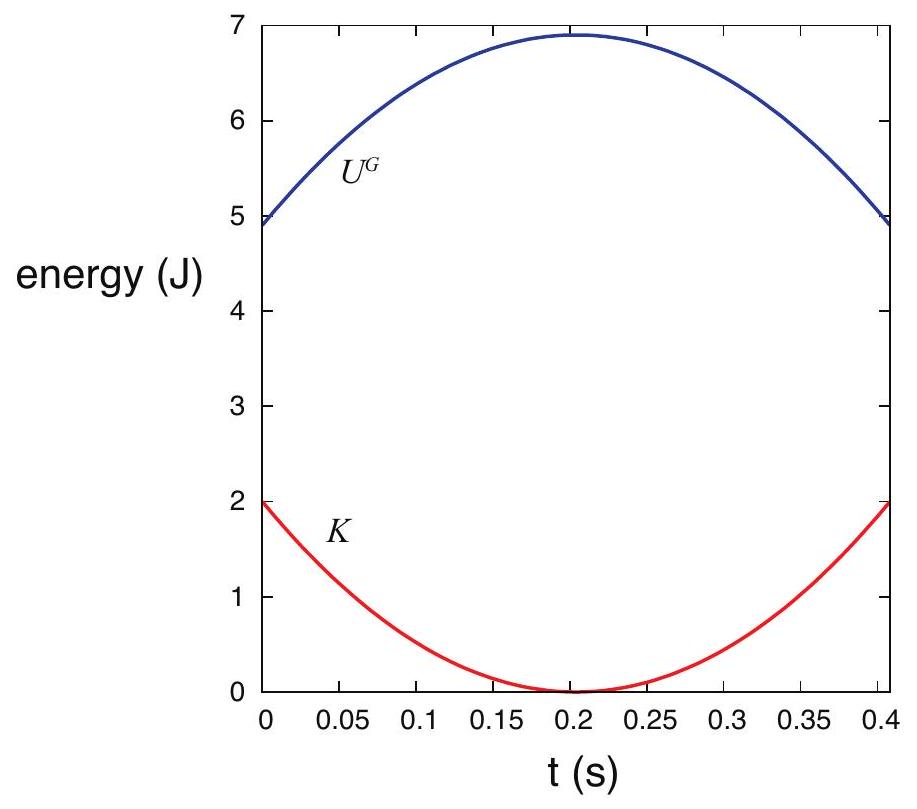
\includegraphics[max width=\textwidth]{2024_09_14_9969b06773f10b6936e8g-109}
\end{center}

Figure 5.1: Potential and kinetic energy as a function of time for a system consisting of the earth and a 1-kg object sent upwards with $v_{i}=2 \mathrm{~m} / \mathrm{s}$ from a height of 0.5 m .

There is something about potential energy that probably needs to be mentioned at this point. Because I have chosen to launch the object from 0.5 m above the ground, and I have chosen to measure $y$ from the ground, I started out with a potential energy of $m g y_{i}=4.9 \mathrm{~J}$. This makes sense, in a way: it tells you that if you simply dropped the object from this height, it would have picked up an amount of kinetic energy equal to 4.9 J by the time it reached the ground. But, actually, where I choose the vertical origin of coordinates is arbitrary. I could start measuring $y$\\
from any height I wanted to-for instance, taking the initial height of my hand to correspond to $y=0$. This would shift the blue curve in Fig. 5.1 down by 4.9 J , but it would not change any of the physics. The only important thing I really want the potential energy for is to calculate the kinetic energy the object will lose or gain as it moves from one height to another, and for that only changes in potential energy matter. I can always add or subtract any (constant) number ${ }^{1}$ to or from $U$, and it will still be true that $\Delta K=-\Delta U$.

What about potential energy in the context in which we first encountered it, that of elastic collisions in one dimension? Imagine that we have two carts collide on an air track, and one of them, let us say cart 2 , is fitted with a spring. As the carts come together, they compress the spring, and some of their kinetic energy is "stored" in it as elastic potential energy. In physics, we use the following expression for the potential energy stored in what we call an ideal spring ${ }^{2}$ :


\begin{equation*}
U^{s p r}(x)=\frac{1}{2} k\left(x-x_{0}\right)^{2} \tag{5.5}
\end{equation*}


where $k$ is something called the spring constant; $x_{0}$ is the "equilibrium length" of the spring (when it is neither compressed nor stretched); and $x$ its actual length, so $x>x_{0}$ means the spring is stretched, and $x<x_{0}$ means it is compressed. For the system of the two carts colliding, we can take the potential energy to be given by Eq. (5.5) if the distance between the carts is less than $x_{0}$, and 0 (corresponding to a relaxed spring) otherwise. If we put cart 1 on the left and cart 2 on the right, then the distance between them is $x_{2}-x_{1}$, and so we can write, for the whole interaction

\[
\begin{array}{rr}
U\left(x_{2}-x_{1}\right)=\frac{1}{2} k\left(x_{2}-x_{1}-x_{0}\right)^{2} & \text { if } x_{2}-x_{1}<x_{0} \\
0 & \text { otherwise } \tag{5.6}
\end{array}
\]

This is enough to solve for the motion of the two carts, given the initial conditions. To see how, look in the "Examples" section at the end of this chapter. Here, I will just give you the result.

For the calculation, shown in Fig. 5.2 below, I have chosen cart 1 to have a mass of 1 kg , an initial position (at $t=0$ ) of $x_{1 i}=-5 \mathrm{~cm}$ and an initial velocity of $1 \mathrm{~m} / \mathrm{s}$, whereas cart 2 has a mass of 2 kg and starts at rest at $x_{2 i}=0$. I have assumed the spring has a length of $x_{0}=2 \mathrm{~cm}$ and a spring constant $k=1000 \mathrm{~J} / \mathrm{m}^{2}$ (which sounds like a lot but isn't really). The collision begins at $t_{c}=\left(x_{2 i}-x_{0}-x_{1 i}\right) / v_{1 i}=0.03 \mathrm{~s}$, which is the time it takes cart 1 to travel the 3 cm separating it from the end of the spring. Prior to that point, the total kinetic energy $K_{\text {sys }}=0.5 \mathrm{~J}$, and the total potential energy $U=0$.

\footnotetext{${ }^{1}$ Of course, some choices may result in the potential energy, and even the total energy, being negative sometimes! If this notion of a negative total energy bothers you a bit, wait until the chapter on gravity (Chapter 10), where we will try to make some sense out of it...\\
${ }^{2}$ An "ideal spring" is basically defined, mathematically, by this expression, or by the corresponding force equation (6.21) (which we will study in the next chapter, and which goes by the name of Hooke's law); usually, we also require that the spring be "massless" (by which we mean that its mass should be negligible compared to all the other masses involved in any given problem). Of course, for Eq. (5.5) to hold for $x<x_{0}$, it must be possible to compress the spring as well as stretch it, which is not always possible with some springs.
}As a result of the collision, the spring compresses and undergoes "half a cycle" of oscillation with an "angular frequency" $\omega=\sqrt{k / \mu}$ (where $\mu$ is, as in previous chapters, the "reduced mass" of the system, $\left.\mu=m_{1} m_{2} /\left(m_{1}+m_{2}\right)\right)$. That is, the spring is compressed and then pushes out until it gets back to its equilibrium length ${ }^{3}$. This lasts from $t=t_{c}$ until $t=t_{c}+\pi / \omega$, during which time the potential and kinetic energies of the system can be written as


\begin{align*}
& U(t)=\frac{1}{2} \mu v_{12, i}^{2} \sin ^{2}\left[\omega\left(t-t_{c}\right)\right] \\
& K(t)=K_{c m}+\frac{1}{2} \mu v_{12, i}^{2} \cos ^{2}\left[\omega\left(t-t_{c}\right)\right] \tag{5.7}
\end{align*}


(don't worry, all this will make a lot more sense after we get to Chapter 11 on simple harmonic motion, I promise!). After $t=t_{c}+\pi / \omega$, the interaction is over, and $K$ and $U$ go back to their initial values.

\begin{center}
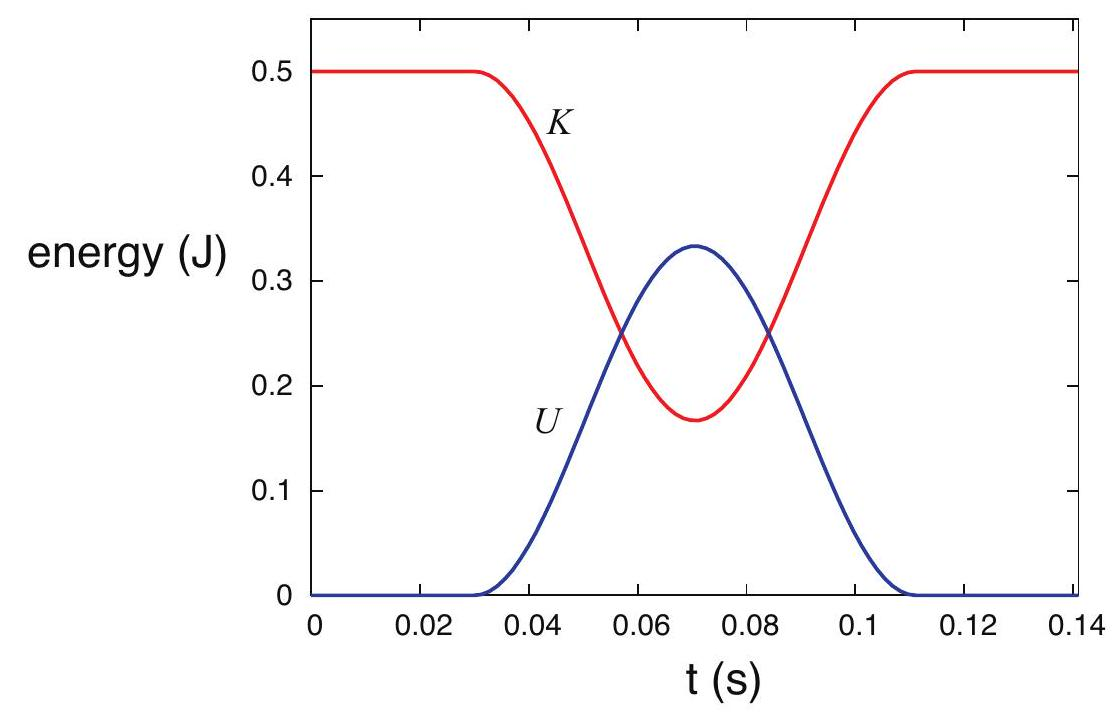
\includegraphics[max width=\textwidth]{2024_09_14_9969b06773f10b6936e8g-111}
\end{center}

Figure 5.2: Potential and kinetic energy as a function of time for a system of two carts colliding and compressing a spring in the process.

If you compare Figure 5.2 with Figure 4.5 of Chapter 4 , you'll see that the kinetic energy curve looks very similar, except for the time scale, which here is hundredths of a second and over there was taken to be milliseconds. The quantity that determines the time scale here is the "half period" of oscillation, $\pi / \omega=\pi \sqrt{\mu / k}=0.081 \mathrm{~s}$ for the values of $k$ and $\mu$ assumed here. We could make this smaller by making the spring stiffer (increasing $k$ ), or the blocks lighter (reducing $\mu$ ), but there's not much point in trying, since the collisions in Chapters 3 and 4 were all just made up in any case.

\footnotetext{${ }^{3}$ As noted earlier, we shall always assume our springs to be "massless," that is, that their inertia is negligible. In turn, negligible inertia means that the spring does not "keep going": it stops stretching as soon as it is back to its original length.
}The main point is that this kind of physical setup (a cart fitted with a spring) would indeed give us an elastic collision, and a kinetic energy curve very much like the ones I used, for illustration purposes, in Chapter 4; only now we also have a potential energy curve to go with it, and to show where the energy is "hiding" while the collision lasts.\\
(You might wonder, anyway, what kind of potential energy function would actually produce the made-up elastic collision curves in Chapters 3 and 4? The (perhaps surprising) answer is, I do not really know, and I have no way to find out! If you are curious about why, again look at the "Examples" section at the end of the chapter.)

\subsection*{5.1.2 Potential energy functions and "energy landscapes"}
The potential energy function of a system, as illustrated in the above examples, serves to let us know how much energy can be stored in, or extracted from, the system by changing its configuration, that is to say, the positions of its parts relative to each other. We have seen this in the case of the gravitational force (the "configuration" in this case being the distance between the object and the earth), and just now in the case of a spring (how stretched or compressed it is). In all these cases we should think of the potential energy as being a property of the system as a whole, not any individual part; it is, very loosely speaking, something akin to a "stress" in the system that can be turned into motion under the right conditions.

It is a consequence of the principle of conservation of momentum that, if the interaction between two particles can be described by a potential energy function, this should be a function only of their relative position, that is, the quantity $x_{1}-x_{2}$ ( or $x_{2}-x_{1}$ ), and not of the individual coordinates, $x_{1}$ and $x_{2}$, separately ${ }^{4}$. The example of the spring in the previous section illustrates this, whereas the gravitational potential energy example shows how this can be simplified in an important case: in Eq. (5.3), the height $y$ of the object above the ground is really a measure of the distance between the object and the earth, something that we could write, in full generality, as $\left|\vec{r}_{o}-\vec{r}_{E}\right|$ (where $\vec{r}_{o}$ and $\vec{r}_{E}$ are the position vectors of the Earth and the object, respectively). However, since we do not expect the Earth to move very much as a result of the interaction, we can take its position to be constant, and only include the position of the object explicitly in our potential energy function, as we did above ${ }^{5}$.

Generally speaking, then, we can identify a large class of problems where a "small" object or "particle" interacts with a much more massive one, and it is a good approximation to write the potential energy of the whole system as a function of only the position of the particle. In one

\footnotetext{${ }^{4}$ We will see why in the next chapter! But, if you want to peek ahead, nothing's preventing you from reading sections 6.1 and 6.2 right now. Basically, to conserve momentum we need Eq. (6.6) to hold, and as you can see from Eq. (6.18), having the potential energy depend only on $x_{1}-x_{2}$ ensures that.\\
${ }^{5}$ This will change in Chapter 10, when we get to study gravity over a planetary scale.
}
dimension, then, we have a situation where, once the initial conditions (the particle's initial position and velocity) are known, the motion of the particle can be completely determined from the function $U(x)$, where $x$ is the particle's position at any given time. This can be done, using calculus, essentially by the method illustrated in Example 5.6.3 at the end of this chapter (namely, let $v= \pm \sqrt{2 m(E-U(x))}$ and solve the resulting differential equation); but it is also possible to get some pretty valuable insights into the particle's motion without using any calculus at all, through a mostly graphical approach that I would like to show you next.

\begin{center}
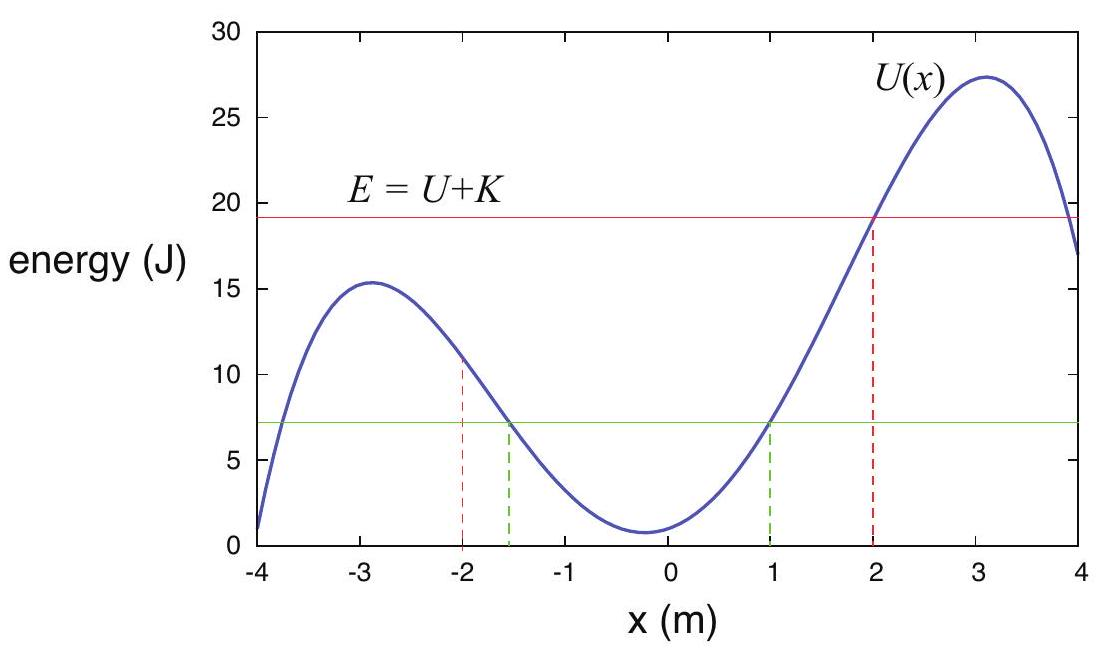
\includegraphics[max width=\textwidth]{2024_09_14_9969b06773f10b6936e8g-113}
\end{center}

Figure 5.3: A hypothetical potential energy curve for a particle in one dimension. The horizontal red line shows the total mechanical energy under the assumption that the particle starts out at $x=-2 \mathrm{~m}$ with $K_{i}=8 \mathrm{~J}$. The green line assumes the particle starts instead from rest at $x=1 \mathrm{~m}$.

In Figure 5.3 above I have assumed, as an example, that the potential energy of the system, as a function of the position of the particle, is given by the function $U(x)=-x^{4} / 4+9 x^{2} / 2+2 x+1$ (in joules, if $x$ is given in meters). Consider then what happens if the particle has a mass $m=4 \mathrm{~kg}$ and is found initially at $x_{i}=-2 \mathrm{~m}$, with a velocity $v_{i}=2 \mathrm{~m} / \mathrm{s}$. (This scenario goes with the red lines in Fig. 5.3, so please ignore the green lines for the time being.) Its kinetic energy will then be $K_{i}=8 \mathrm{~J}$, whereas the potential energy will be $U(-2)=11 \mathrm{~J}$. The total mechanical energy is then $E=19 \mathrm{~J}$, as indicated by the red horizontal line.

Now, as the particle moves, the total energy remains constant, so as it moves to the right, its potential energy goes down at first, and consequently its kinetic energy goes up-that is, it accelerates. At some point, however (around $x=-0.22 \mathrm{~m}$ ) the potential energy starts to go up, and so the particle starts to slow down, although it keeps going, because $K=E-U$ is still nonzero. However, when the particle eventually reaches the point $x=2 \mathrm{~m}$, the potential energy $U(2)=19 \mathrm{~J}$, and the kinetic energy becomes zero.

At that point, the particle stops and turns around, just like an object thrown vertically upwards. As it moves "down the potential energy hill," it recovers the kinetic energy it used to have, so that when it again reaches the starting point $x=-2 \mathrm{~m}$, its speed is again $2 \mathrm{~m} / \mathrm{s}$, but now it is moving in the opposite direction, so it just passes through and over the next "hill" (since it has enough total energy to do so), and eventually moves outside the region shown in the figure.

As another example, consider what would have happened if the particle had been released at, say, $x=1 \mathrm{~m}$, but with zero velocity. (This is illustrated by the green lines in Fig. 5.3.) Then the total energy would be just the potential energy $U(1)=7.25 \mathrm{~J}$. The particle could not possibly move to the right, since that would require the total energy to go up. It can only move to the left, since in that direction $U(x)$ decreases (initially, at first), and that means $K$ can increase (recall $K$ is always positive as long as the particle is in motion). So the particle speeds up to the left until, past the point $x=-0.22 \mathrm{~m}, U(x)$ starts to increase again and $K$ has to go down. Eventually, as the figure shows, we reach a point (which we can calculate to be $x=-1.548 \mathrm{~m}$ ) where $U(x)$ is once again equal to 7.25 J . This leaves no room for any kinetic energy, so the particle has to stop and turn back. The resulting motion consists of the particle oscillating back and forth forever between $x=-1.548 \mathrm{~m}$ and $x=1 \mathrm{~m}$.

At this point, you may have noticed that the motion I have described as following from the $U(x)$ function in Figure 5.3 resembles very much the motion of a car on a roller-coaster having the shape shown, or maybe a ball rolling up and down hills like the ones shown in the picture. In fact, the correspondence can be made exact-if we substitute sliding for rolling, since rolling motion has complications of its own. Given an arbitrary potential energy function $U(x)$ for a particle of mass $m$, imagine that you build a "landscape" of hills and valleys whose height $y$ above the horizontal, for a given value of the horizontal coordinate $x$, is given by the function $y(x)=U(x) / m g$. (Note that $m g$ is just a constant scaling factor that does not change the shape of the curve.) Then, for an object of mass $m$ sliding without friction over that landscape, under the influence of gravity, the gravitational potential energy at any point $x$ would be $U^{G}(x)=m g y=U(x)$, and therefore its speed at any point will be precisely the same as that of the original particle, if it starts at the same point with the same velocity.

This notion of an "energy landscape" can be extended to more than one dimension (although they are hard to visualize in three!), or generalized to deal with configuration parameters other than a single particle's position. It can be very useful in a number of disciplines (not just physics), to predict the ways in which the configuration of a system may be likely to change.

\subsection*{5.2 Dissipation of energy and thermal energy}
From all the foregoing, it is clear that when an interaction can be completely described by a potential energy function we can define a quantity, which we have called the total mechanical\\
energy of the system, $E_{\text {mech }}=K+U$, that is constant throughout the interaction. However, we already know from our study of inelastic collisions that this is rarely the case. Essential to the concept of potential energy is the idea of "storage and retrieval" of the kinetic energy of the system during the interaction process. When kinetic energy simply disappears from the system and does not come back, a full description of the process in terms of a potential energy is not possible.

Processes in which some amount of mechanical energy disappears (that is, it cannot be found anywhere anymore as either macroscopic kinetic or potential energy) are called dissipative. Mysterious as they may appear at first sight, there is actually a simple, intuitive explanation for them. All macroscopic systems consist of a great number of small parts that enjoy, at the microscopic level, some degree of independence from each other and from the body to which they belong. Macroscopic motion of an object requires all these parts to move together as a whole, at least on average; however, a collision with another object may very well "rattle" all these parts and leave them in a more or less disorganized state. If the total energy is conserved, then after the collision the object's atoms or molecules may be, on average, vibrating faster or banging against each other more often than before, but they will do so in random directions, so this increased "agitation" will not be perceived as macroscopic motion of the object as a whole.

This kind of random agitation at the microscopic level that I have just introduced is what we know today as thermal energy, and it is by far the most common "sink" or reservoir where macroscopic mechanical energy is "dissipated." In our example of an inelastic collision, the energy the objects had is not gone from the universe, in fact it is still right there inside the objects themselves; it is just in a disorganized or incoherent state from which, as you can imagine, it would be pretty much impossible to retrieve it, since we would have to somehow get all the randomly-moving parts to get back to moving in the same direction again.

We will have a lot more to say about thermal energy in a later chapter, but for the moment you may want to think of it as essentially noise: it is what is left (the residual motional or configurational energy, at the microscopic level) after you remove the average, macroscopically-observable kinetic or potential energy. So, for example, for a solid object moving with a velocity $v_{c m}$, the kinetic part of its thermal energy would be the sum of the kinetic energies of all its microscopic parts, calculated in its center of mass (or zero-momentum) reference frame; that way you remove from every molecule's velocity the quantity $v_{c m}$, which they all must have in common - on average (since the body as a whole is moving with that velocity) ${ }^{6}$.

In order to establish conservation of energy as a fact (which was one of the greatest scientific triumphs of the 19th century) it was clearly necessary to show experimentally that a certain amount

\footnotetext{${ }^{6}$ Note that thermal energy is not necessarily just kinetic; it may have a configurational component to it as well. For example, imagine a collection of vibrating diatomic molecules. You may think of each one as two atoms connected by a spring. The length of the "spring" at rest determines the molecule's nominal chemical energy; thermal vibrations cause this length to change, resulting in a net increase in energy that - as for two masses connected by a spring-has both a kinetic and a configurational (or "potential") component.
}
of mechanical energy lost always resulted in the same predictable increase in the system's thermal energy. Thermal energy is largely "invisible" at the macroscopic level, but we detect it indirectly through an object's temperature. The crucial experiments to establish what at the time was called the "mechanical equivalent of heat" were carried out by James Prescott Joule in the 1850's, and required exceedingly precise measurements of temperature (in fact, getting the experiments done was only half the struggle; the other half was getting the scientific establishment to believe that he could measure changes in temperature so accurately!)

\subsection*{5.3 Fundamental interactions, and other forms of energy}
At the most fundamental (microscopic) level, physicists today believe that there are only four (or three, depending on your perspective) basic interactions: gravity, electromagnetism, the strong nuclear interaction (responsible for holding atomic nuclei together), and the weak nuclear interaction (responsible for certain nuclear processes, such as the transmutation of a proton into a neutron ${ }^{7}$ and vice-versa). In a technical sense, at the quantum level, electromagnetism and the weak nuclear interactions can be regarded as separate manifestations of a single, consistent quantum field theory, so they are sometimes referred to as "the electroweak interaction."

All of these interactions are conservative, in the sense that for all of them one can define the equivalent of a "potential energy function" (generalized, as necessary, to conform to the requirements of quantum mechanics and relativity), so that for a system of elementary particles interacting via any one of these interactions the total kinetic plus potential energy is a constant of the motion. For gravity (which we do not really know how to "quantize" anyway!), this function immediately carries over to the macroscopic domain without any changes, as we shall see in a later chapter, and the gravitational potential energy function I introduced earlier in this chapter is an approximation to it valid near the surface of the earth (gravity is such a weak force that the gravitational interaction between any two earth-bound objects is virtually negligible, so we only have to worry about gravitational energy when one of the objects involved is the earth itself).

As for the strong and weak nuclear interactions, they are only appreciable over the scale of an atomic nucleus, so there is no question of them directly affecting any macroscopic mechanical processes. They are responsible, however, for various nuclear reactions in the course of which nuclear energy is, most commonly, transformed into electromagnetic energy (X- or gamma rays) and thermal energy.

All the other forms of energy one encounters at the microscopic, and even the macroscopic, level have their origin in electromagnetism. Some of them, like the electrostatic energy in a capacitor or the magnetic interaction between two permanent magnets, are straightforward enough scale-ups of their microscopic counterparts, and may allow for a potential energy description at the macroscopic

\footnotetext{${ }^{7}$ Plus a positron and a neutrino.
}
level (and you will learn more about them next semester!). Many others, however, are more subtle and involve quantum mechanical effects (such as the exclusion principle) in a fundamental way.

Among the most important of these is chemical energy, which is an extremely important source of energy for all kinds of macroscopic processes: combustion (and explosions!), the production of electrical energy in batteries, and all the biochemical processes that power our own bodies. However, the conversion of chemical energy into macroscopic mechanical energy is almost always a dissipative process (that is, one in which some of the initial chemical energy ends up irreversibly converted into thermal energy), so it is generally impossible to describe them using a (macroscopic) potential energy function (except, possibly, for electrochemical processes, with which we will not be concerned here).

For instance, consider a chemical reaction in which some amount of chemical energy is converted into kinetic energy of the molecules forming the reaction products. Even when care is taken to "channel" the motion of the reaction products in a particular direction (for example, to push a cylinder in a combustion engine), a lot of the individual molecules will end up flying in the "wrong" direction, striking the sides of the container, etc. In other words, we end up with a lot of the chemical energy being converted into disorganized microscopic agitation-which is to say, thermal energy.

Electrostatic and quantum effects are also responsible for the elastic properties of materials, which can sometimes be described by macroscopic potential energy functions, at least to a first approximation (like the spring we studied earlier in the chapter). They are also responsible for the adhesive forces between surfaces that play an important role in friction, and various other kinds of what might be called "structural energies," most of which play only a relatively small part in the energy balance where macroscopic objects are involved.

\subsection*{5.4 Conservation of energy}
Today, physics is pretty much founded on the belief that the energy of a closed system (defined as one that does not exchange energy with its surroundings-more on this in a minute) is always conserved: that is, internal processes and interactions will only cause energy to be "converted" from one form into another, but the total, after all the forms of energy available to the system have been carefully accounted for, will not change. This belief is based on countless experiments, on the one hand, and, on the other, on the fact that all the fundamental interactions that we are aware of do conserve a system's total energy.

Of course, recognizing whether a system is "closed" or not depends on having first a complete catalogue of all the ways in which energy can be stored and exchanged - to make sure that there is, in fact, no exchange of energy going on with the surroundings. Note, incidentally, that a "closed"\\
system is not necessarily the same thing as an "isolated" system: the former relates to the total energy, the latter to the total momentum. A parked car getting hotter in the sun is not a closed system (it is absorbing energy all the time) but, as far as its total momentum is concerned, it is certainly fair to call it "isolated." (And as you keep this in mind, make sure you also do not mistake "isolated" for "insulated"!) Hopefully all these concepts will be further clarified when we introduce the additional auxiliary concepts of force, work, and heat (although the latter will not come until the end of the semester).

For a closed system, we can state the principle of conservation of energy (somewhat symbolically) in the form


\begin{equation*}
K+U+E_{\text {source }}+E_{\text {diss }}=\mathrm{constant} \tag{5.8}
\end{equation*}


where $K$ is the total, macroscopic, kinetic energy; $U$ the sum of all the applicable potential energies associated with the system's internal interactions; $E_{\text {source }}$ is any kind of internal energy (such as chemical energy) that is not described by a potential energy function, but can increase the system's mechanical energy; and $E_{\text {diss }}$ stands for the contents of the "dissipated energy reservoir" - typically thermal energy. As with the potential energy $U$, the absolute value of $E_{\text {source }}$ and $E_{\text {diss }}$ does not (usually) really matter: all we are interested in is how much they change in the course of the process under consideration.

\begin{center}
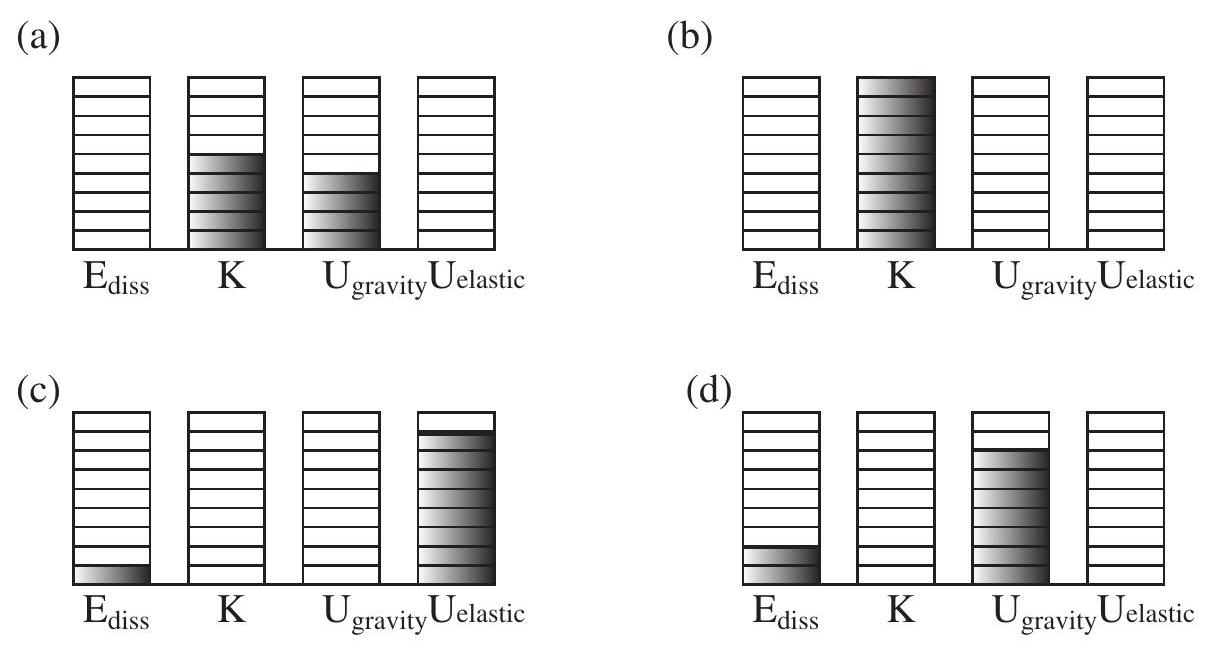
\includegraphics[max width=\textwidth]{2024_09_14_9969b06773f10b6936e8g-118}
\end{center}

Figure 5.4: Energy bar diagrams for a system formed by the earth and a ball thrown downwards. (a) As the ball leaves the hand. (b) Just before it hits the ground. (c) During the collision, at the time of maximum compression. (d) At the top of the first bounce. The total number of energy "units" is the same in all the diagrams, as required by the principle of conservation of energy. From the diagrams you can tell that the coefficient of restitution $e=\sqrt{7 / 9}$.

Figure 5.4 above is an example of this kind of "energy accounting" for a ball bouncing on the ground. If the ball is thrown down, the system formed by the ball and the earth initially has both\\
gravitational potential energy, and kinetic energy (diagram (a)). Note that we could write the total kinetic energy as $K_{c m}+K_{c o n v}$, as we did in the previous chapter, but because of the large mass of the earth, the center of mass of the system is essentially the center of the earth, which, in our earth-bound coordinate system, does not move at all, so $K_{c m}$ is, to an excellent approximation, zero. Then, the reduced mass of the system, $\mu=m_{b} M_{E} /\left(m_{b}+M_{E}\right)$ is, also to an excellent approximation, just equal to the mass of the ball, so $K_{\text {conv }}=\frac{1}{2} \mu v_{12}^{2}=\frac{1}{2} m_{b}\left(v_{b}-v_{e}\right)^{2}=\frac{1}{2} m_{b} v_{b}^{2}$ (again, because the earth does not move). So all the kinetic energy that we have is the kinetic energy of the ball, and it is all, in principle, convertible (as you can see if you replace the ball, for instance, with a bean bag).

As the ball falls, gravitational potential energy is being converted into kinetic energy, and the ball speeds up. As it is about to hit the ground (diagram (b)), the potential energy is zero and the kinetic energy is maximum. During the collision with the ground, all the kinetic energy is temporarily converted into other forms of energy, which are essentially elastic energy of deformation (like the energy in a spring) and some thermal energy (diagram (c)). When it bounces back, its kinetic energy will only be a fraction $e^{2}$ of what it had before the collision (where $e$ is the coefficient of restitution). This kinetic energy is all converted into gravitational potential energy as the ball reaches the top of its bounce (diagram (d)). Note there is more dissipated energy in diagram (d) than in (c); this is because I have assumed that dissipation of energy takes place both during the compression and the subsequent expansion of the ball.

\subsection*{5.5 In summary}
\begin{enumerate}
  \item For conservative interactions one can define a potential energy $U$, such that that in the course of the interaction the total mechanical energy $E=U+K$ of the system remains constant, even as $K$ and $U$ separately change. The function $U$ is a measure of the energy stored in the configuration of the system, that is, the relative position of all its parts.
  \item The potential energy function for a system of two particles must be a function of their relative position only: $U\left(x_{1}-x_{2}\right)$. However, if one of the objects is very massive, so it does not move during the interaction, its position may be taken to be the origin of coordinates, and $U$ written as a function of the lighter object's coordinate alone.
  \item For a system formed by the earth and an object of mass $m$ at a height $y$ above the ground, the gravitational potential energy can be written as $U^{G}=m g y$ (approximately, as long as $y$ is much smaller than the radius of the earth).
  \item The elastic potential energy stored in an ideal spring of spring constant $k$ and relaxed length $x_{0}$, when stretched or compressed to an actual length $x$, is $U^{s p r}=\frac{1}{2} k\left(x-x_{0}\right)^{2}$.
  \item For an object in one dimension, with position coordinate $x$, which is part of a system with potential energy $U(x)$, the motion can be predicted from the "energy landscape" formed by\\
the graph of the function $U(x)$. The idea, elaborated in Section 5.1.2 above, is to imagine the equivalent motion of an object sliding without friction over the same landscape, under the influence of gravity.
  \item The fundamental interactions currently known in physics are gravity, the strong nuclear interaction and the electroweak interaction (which includes all electromagnetic phenomena). These are all conservative.
  \item At a macroscopic level, one finds a number of interactions and associated energies that are derived from electromagnetism and quantum mechanics. Two important examples are chemical energy, and elastic energy (which is energy associated with the elasticity or "springiness" of a body). Elastic energy can often be described approximately by a potential energy function, and as such be included in calculations of the total mechanical energy of a system.
  \item Interactions between macroscopic objects almost always involve the conversion of some type of energy into another. Typically, some of the total mechanical energy is always lost in the conversion process, because it is impossible to keep at least some of the energy from spreading itself randomly among the microscopic parts that make up the interacting objects. This is an intrinsically irreversible process known as dissipation of energy.
  \item Most of the time the dissipated energy ends up as thermal energy, which is energy associated with a random agitation at the atomic or molecular level.
  \item A closed system is one that does not exchange energy with its surrounding. This is not necessarily the same thing as an isolated system (which is one that does not exchange momentum with its surroundings). For a closed system, the sum of its macroscopic mechanical energy (kinetic + potential) and all its other "internal" energies (chemical, thermal), must be a constant.
\end{enumerate}

\subsection*{5.6 Examples}
\subsection*{5.6.1 Inelastic collision in the middle of a swing}
Tarzan swings on a vine to rescue a helpless explorer (as usual) from some attacking animal or another. He begins his swing from a branch a height of 15 m above the ground, grabs the explorer at the bottom of his swing, and continues the swing, upwards this time, until they both land safely on another branch. Suppose that Tarzan weighs 90 kg and the explorer weighs 70 , and that Tarzan doesn't just drop from the branch, but pushes himself off so that he starts the swing with a speed of $5 \mathrm{~m} / \mathrm{s}$. How high a branch can he and the explorer reach?

\section*{Solution}
Let us break this down into parts. The first part of the swing involves the conversion of some amount of initial gravitational potential energy into kinetic energy. Then comes the collision with the explorer, which is completely inelastic and we can analyze using conservation of momentum (assuming Tarzan and the explorer form an isolated system for the brief time the collision lasts). After that, the second half of their swing involves the complete conversion of their kinetic energy into gravitational potential energy.

Let $m_{1}$ be Tarzan's mass, $m_{2}$ the explorer's mass, $h_{i}$ the initial height, and $h_{f}$ the final height. We also have three velocities to worry about (or, more properly in this case, speeds, since their direction is of no concern, as long as they all point the way they are supposed to): Tarzan's initial velocity at the beginning of the swing, which we may call $v_{\text {top }}$; his velocity at the bottom of the swing, just before he grabs the explorer, which we may call $v_{b o t 1}$, and his velocity just after he grabs the explorer, which we may call $v_{\text {bot2 }}$. (If you find those subscripts confusing, I am sorry, they are the best I could do; please feel free to make up your own.)

\begin{itemize}
  \item First part: the downswing. We apply conservation of energy, in the form (5.8), to the first part of the swing. The system we consider consists of Tarzan and the earth, and it has kinetic energy as well as gravitational potential energy. We ignore the source energy and the dissipated energy terms, and consider the system closed despite the fact that Tarzan is holding onto a vine (as we shall see in a couple of chapters, the vine does no "work" on Tarzan - meaning, it does not change his energy, only his direction of motion-because the force it exerts on Tarzan is always perpendicular to his displacement):
\end{itemize}


\begin{equation*}
K_{\text {top }}+U_{\text {top }}^{G}=K_{\text {bot } 1}+U_{\text {bot }}^{G} \tag{5.9}
\end{equation*}


In terms of the quantities I introduced above, this equation becomes:

$$
\frac{1}{2} m_{1} v_{\text {top }}^{2}+m_{1} g h_{i}=\frac{1}{2} m_{1} v_{b o t 1}^{2}+0
$$

which can be solved to give


\begin{equation*}
v_{\text {bot1 }}^{2}=v_{\text {top }}^{2}+2 g h_{i} \tag{5.10}
\end{equation*}


(note that this is just the familiar result (2.10) for free fall! This is because, as I pointed out above, the vine does no work on the system.). Substituting, we get

$$
v_{\text {bot } 1}=\sqrt{\left(5 \frac{\mathrm{m}}{\mathrm{s}}\right)^{2}+2\left(9.8 \frac{\mathrm{m}}{\mathrm{s}^{2}}\right) \times(15 \mathrm{~m})}=17.9 \frac{\mathrm{m}}{\mathrm{s}}
$$

\begin{itemize}
  \item Second part: the completely inelastic collision. The explorer is initially at rest (we assume he has not seen the wild beast ready to pounce yet, or he has seen it and he is paralyzed by fear!). After Tarzan grabs him they are moving together with a speed $v_{\text {bot2 }}$. Conservation of momentum gives
\end{itemize}


\begin{equation*}
m_{1} v_{\text {bot } 1}=\left(m_{1}+m_{2}\right) v_{\text {bot } 2} \tag{5.11}
\end{equation*}


which we can solve to get

$$
v_{\text {bot } 2}=\frac{m_{1} v_{\text {bot } 1}}{m_{1}+m_{2}}=\frac{(90 \mathrm{~kg}) \times(17.9 \mathrm{~m} / \mathrm{s})}{160 \mathrm{~kg}}=10 \frac{\mathrm{m}}{\mathrm{s}}
$$

\begin{itemize}
  \item Third part: the upswing. Here we use again conservation of energy in the form
\end{itemize}


\begin{equation*}
K_{b o t 2}+U_{b o t}^{G}=K_{f}+U_{f}^{G} \tag{5.12}
\end{equation*}


where the subscript $f$ refers to the very end of the swing, when they both safely reach their new branch, and all their kinetic energy has been converted to gravitational potential energy, so $K_{f}=0$ (which means that is as high as they can go, unless they start climbing the vine!). This equation can be rewritten as

$$
\frac{1}{2}\left(m_{1}+m_{2}\right) v_{b o t 2}^{2}+0=0+\left(m_{1}+m_{2}\right) g h_{f}
$$

and solving for $h_{f}$ we get

$$
h_{f}=\frac{v_{b o t 2}^{2}}{2 g}=\frac{(10 \mathrm{~m} / \mathrm{s})^{2}}{2 \times 9.8 \mathrm{~m} / \mathrm{s}^{2}}=5.15 \mathrm{~m}
$$

\subsection*{5.6.2 Kinetic energy to spring potential energy: block collides with spring}
A block of mass $m$ is sliding on a frictionless, horizontal surface, with a velocity $v_{i}$. It hits an ideal spring, of spring constant $k$, which is attached to the wall. The spring compresses until the block momentarily stops, and then starts expanding again, so the block ultimately bounces off.\\
(a) In the absence of dissipation, what is the block's final speed?\\
(b) By how much is the spring compressed?

\section*{Solution}
This is a simpler version of the problem considered in Section 5.1.1, and in the next example. The\\
problem involves the conversion of kinetic energy into elastic potential energy, and back. In the absence of dissipation, Eq. (5.8), specialized to this system (the spring and the block) reads:


\begin{equation*}
K+U^{s p r}=\text { constant } \tag{5.13}
\end{equation*}


For part (a), we consider the whole process where the spring starts relaxed and ends relaxed, so $U_{i}^{s p r}=U_{f}^{s p r}=0$. Therefore, we must also have $K_{f}=K_{i}$, which means the block's final speed is the same as its initial speed. As explained in the chapter, this is characteristic of a conservative interaction.

For part (b), we take the final state to be the instant where the spring is maximally compressed and the block is momentarily at rest, so all the energy in the system is spring (which is to say, elastic) potential energy. If the spring is compressed a distance $d$ (that is, $x-x_{0}=-d$ in Eq. (5.5)), this potential energy is $\frac{1}{2} k d^{2}$, so setting that equal to the system's initial energy we get:


\begin{equation*}
K_{i}+0=0+\frac{1}{2} k d^{2} \tag{5.14}
\end{equation*}


or

$$
\frac{1}{2} m v_{i}^{2}=\frac{1}{2} k d^{2}
$$

which can be solved to get

$$
d=\sqrt{\frac{m}{k}} v_{i}
$$

\subsection*{5.7 Advanced Topics}
\subsection*{5.7.1 Two carts colliding and compressing a spring}
Unlike the example 5.6.2, which considered a stationary spring and asked only questions about initial and final states, this example is intended to show you how one can use "energy methods" to solve for the actual motion of a relatively complicated system as a function of time. The system is the two carts colliding, one of them fitted with a spring, considered in Section 5.1.1. Although all the physics involved is straightforward, the math is at a higher level than you will be using this semester, so I'm presenting this here as a "curiosity" only.

First, recall the total kinetic energy for a collision problem can be written as $K=K_{c m}+K_{c o n v}$, where (if the system is isolated) $K_{c m}$ remains constant throughout. Then, the total mechanical energy $E=K+U=K_{c m}+K_{\text {conv }}+U$. This is also constant, and before the interaction happens, when $U=0$, we have $E=K_{c m}+K_{\text {conv, }, i}$, so setting these two things equal and canceling out $K_{c m}$ we get


\begin{equation*}
K_{\text {conv }}=K_{\text {conv }, i}-U \tag{5.15}
\end{equation*}


where the potential energy function is given by Eq. (5.6). Introducing the relative coordinate $x_{12}=x_{2}-x_{1}$, and the relative velocity $v_{12}$, Eq. (5.15) becomes


\begin{equation*}
\frac{1}{2} \mu v_{12}^{2}=\frac{1}{2} \mu v_{12, i}^{2}-\frac{1}{2} k\left(x_{12}-x_{0}\right)^{2} \tag{5.16}
\end{equation*}


an equation that must hold while the interaction is going on. We can solve this for $v_{12}$, and then notice that both $x_{12}$ and $v_{12}$ are functions of time, and the latter is the derivative with respect to time of the former, so


\begin{align*}
v_{12} & = \pm \sqrt{v_{12, i}^{2}-(k / \mu)\left(x_{12}-x_{0}\right)^{2}}  \tag{5.17}\\
\frac{d x_{12}}{d t} & = \pm \sqrt{v_{12, i}^{2}-(k / \mu)\left(x_{12}(t)-x_{0}\right)^{2}} \tag{5.18}
\end{align*}


(The " $\pm$ " sign means that the quantity on the right-hand side has to be negative at first, when the carts are coming together, and positive later, when they are coming apart. This is because I have assumed cart 1 starts to the left of cart 2 , so going in cart 2 , as seen from cart 1, appears to be moving to the left.)

Equation (5.18) is what is known, in calculus, as a differential equation. The problem is to find a function of $t, x_{12}(t)$, such that when you take its derivative you get the expression on the right-hand side. If you know how to calculate derivatives, you can check that the solution is in fact


\begin{equation*}
x_{12}(t)=x_{0}-\frac{v_{12, i}}{\omega} \sin \left[\omega\left(t-t_{c}\right)\right] \quad \text { for } t_{c} \leq t \leq t_{c}+\pi / \omega \tag{5.19}
\end{equation*}


where the quantity $\omega=\sqrt{k / \mu}$, and the time $t_{c}$ is the time cart 1 first makes contact with the spring: $t_{c}=\left(x_{2 i}-x_{0}-x_{1 i}\right) / v_{1 i}$. The solution (5.19) is valid for as long as the spring is compressed, which is to say, for as long as $x_{12}(t)<x_{0}$, or $\sin \left[\omega\left(t-t_{c}\right)\right]>0$, which translates to the condition on $t$ shown above.

Having a solution for $x_{12}$, we could now obtain explicit results for $x_{1}(t)$ and $x_{2}(t)$ separately, using the fact that $x_{1}=x_{c m}-m_{2} x_{12} /\left(m_{1}+m_{2}\right)$, and $x_{2}=x_{c m}+m_{1} x_{12} /\left(m_{1}+m_{2}\right)$ (compare Eqs. (4.10), in chapter 4 ), and finding the position of the center of mass as a function of time is a trivial problem, since it just moves with constant velocity.

We do not, however, need to do any of this in order to generate the plots of the kinetic and potential energy shown in Fig. 5.2: the potential energy depends only on $x_{2}-x_{1}$, which is given explicitly by Eq. (5.19), and the kinetic energy is equal to $K_{c m}+K_{\text {conv }}$, where $K_{c m}$ is constant and $K_{\text {conv }}$ is given by Eq. (5.16), which can also be easily rewritten in terms of Eq. (5.19). The results are Eqs. (5.7) in the text.

\subsection*{5.7.2 Getting the potential energy function from collision data}
Consider the collision illustrated in Figure 3.4 (back in Chapter 3). Can we tell what the potential energy function is for the interaction between the two carts?

At first sight, it may seem that all the information necessary to "reconstruct" the function $U\left(x_{1}-x_{2}\right)$ is available already, at least in graphical form: From Figure 3.4 you could get the value of $x_{2}-x_{1}$ at any time $t$; then from Figure 4.5 you can get the value of $K$ (in the elastic-collision scenario) for the same value of $t$; and then you could plot $U=E-K$ (where $E$ is the total energy) as a function of $x_{2}-x_{1}$.

But there is a catch: Figure 3.4 shows that the colliding objects never get any closer than $x_{2}-x_{1} \simeq$ 0.28 mm , so we have no way to tell what $U\left(x_{2}-x_{1}\right)$ is for smaller values of $x_{2}-x_{1}$. This is essentially the problem faced by particle physicists when they use collisions (which they do regularly) to try to determine the precise nature of the interactions between the particles they study!

You can check this for yourself. The functions I used for $x_{1}(t)$ and $x_{2}(t)$ in figure 3.4 are


\begin{align*}
& x_{1}(t)=\frac{1}{3}\left((2 t-10) \operatorname{erf}(10-2 t)+10 \operatorname{erf}(10)+t-\frac{e^{-4(t-5)^{2}}}{\sqrt{\pi}}\right)-5 \\
& x_{2}(t)=\frac{1}{3}\left((5-t) \operatorname{erf}(10-2 t)-5 \operatorname{erf}(10)+t+\frac{e^{-4(t-5)^{2}}}{2 \sqrt{\pi}}\right) \tag{5.20}
\end{align*}


Here, "erf" is the so-called "error function," which you can find in any decent library of mathemat-\\
ical functions. This looks complicated, but it just gives you the shapes you want for the velocity curves. The derivative of the above is


\begin{align*}
& v_{1}(t)=\frac{1}{3}(1+2 \operatorname{erf}(10-2 t)) \\
& v_{2}(t)=\frac{1}{3}(1-\operatorname{erf}(10-2 t)) \tag{5.21}
\end{align*}


and you may want to try plotting these for yourself; the result should be Figure 3.1.\\
Now, assume (as I did for figure 4.5) that $m_{1}=1 \mathrm{~kg}$, and $m_{2}=2 \mathrm{~kg}$, and use these values and the results (5.21) (assumed to be in $\mathrm{m} / \mathrm{s}$ ) to calculate $K_{\text {sys }}$ as a function of $t$. Then $U=E_{\text {sys }}-K_{\text {sys }}$, with $E_{\text {sys }}=1 / 2 \mathrm{~J}$ :


\begin{equation*}
U=\frac{1}{2}-\frac{1}{2} m_{1} v_{1}^{2}(t)-\frac{1}{2} m_{2} v_{2}^{2}(t)=\frac{1}{3}\left(1-\operatorname{erf}^{2}(10-2 t)\right) \tag{5.22}
\end{equation*}


and now do a parametric plot of $U$ versus $x_{2}-x_{1}$, using $t$ as a parameter. You will end up with a figure like the one below:

\begin{center}
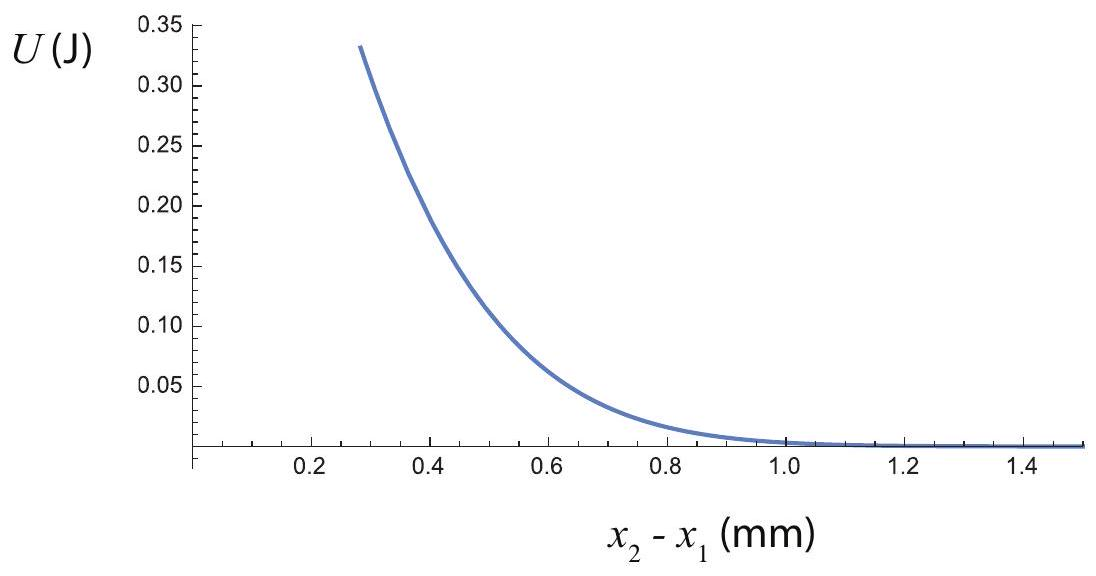
\includegraphics[max width=\textwidth]{2024_09_14_9969b06773f10b6936e8g-126}
\end{center}

Figure 5.5: The potential energy function reconstructed from the information available for the collision shown in Figs. 3.1, 3.4, 4.5. No information can be gathered from those figures (nor from the explicit expressions (5.20) and (5.21) above) on the values of $U$ for $x_{2}-x_{1}<0.28 \mathrm{~mm}$, the distance of closest approach of the two carts.

\subsection*{5.8 Problems}
\section*{Problem 1}
A particle is in a region where the potential energy has the form $U=5 / x$ (in joules, if $x$ is in meters).\\
(a) Sketch this potential energy function for $x>0$.\\
(b) Assuming the particle starts at rest at $x=0.5 \mathrm{~m}$, which way will it go if released? Why?\\
(c) Under the assumption in part (b), what will be the particle's kinetic energy after it has moved 0.1 m from its original position?\\
(d) Now assume that initially the particle is at $x=1 \mathrm{~m}$, moving towards the left with an initial velocity $v_{i}=2 \mathrm{~m} / \mathrm{s}$. If the mass of the particle is 1 kg , how close to the origin can it get before it stops?

\section*{Problem 2}
A "ballistic pendulum" is a device (now largely obsolete, but very useful in its day) to measure the speed of a bullet as it hits a target. Let the target be a block of wood suspended from a string, as in the figure below. When the bullet hits, it is embedded in the wood, and together they swing, like a pendulum, to some maximum height $h$. The question is, how do you find the initial speed of the bullet $\left(v_{i}\right)$ if you know the mass of the bullet $\left(m_{1}\right)$, the mass of the block $\left(m_{2}\right)$, and the height $h ?$

\begin{center}
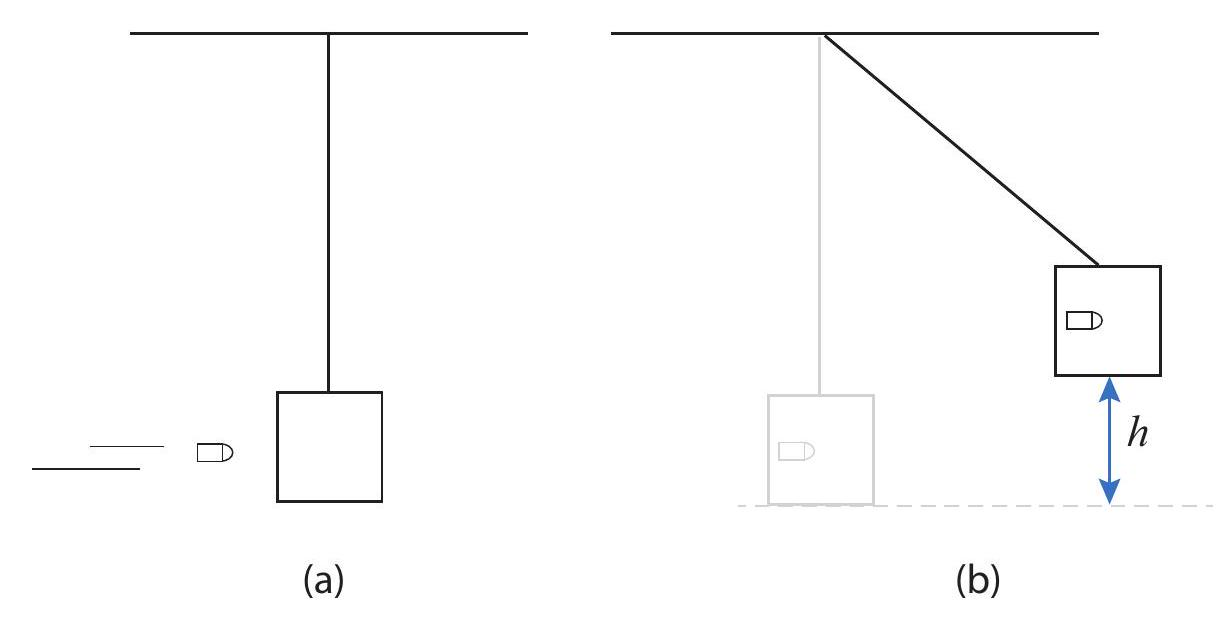
\includegraphics[max width=\textwidth]{2024_09_14_9969b06773f10b6936e8g-127}
\end{center}

Figure 5.6: Ballistic pendulum. (a) Before the bullet hits. (b) After the bullet hits and is embedded in the block, at the maximum height of the swing.

\section*{Problem 3}
You drop a 0.5 kg ball from a height of 2 m , and it bounces back to a height of 1.5 m . Consider the system formed by the ball and the Earth, so we can speak properly of its gravitational potential\\
energy.\\
(a) What is the kinetic energy of the ball just before it hits the ground?\\
(b) What is the kinetic energy of the ball just after it bounces up?\\
(c) What is the coefficient of restitution for this collision?\\
(d) What kind of collision is this (elastic, inelastic, etc.)? Why?\\
(e) If the coefficient of restitution does not change, how high would the ball rise on a second bounce?\\
(f) On the graphs below, draw the energy bar diagrams for the system: (1) as the ball leaves your hand; (2) just before it hits the ground (assume $h=0$ for practical purposes); (3) just after it leaves the ground on its way up ( $h=0$ still), and (4) at the top of its (first) bounce. Make sure to do this to scale, consistent with the values for the energies you have calculated above.

\begin{center}
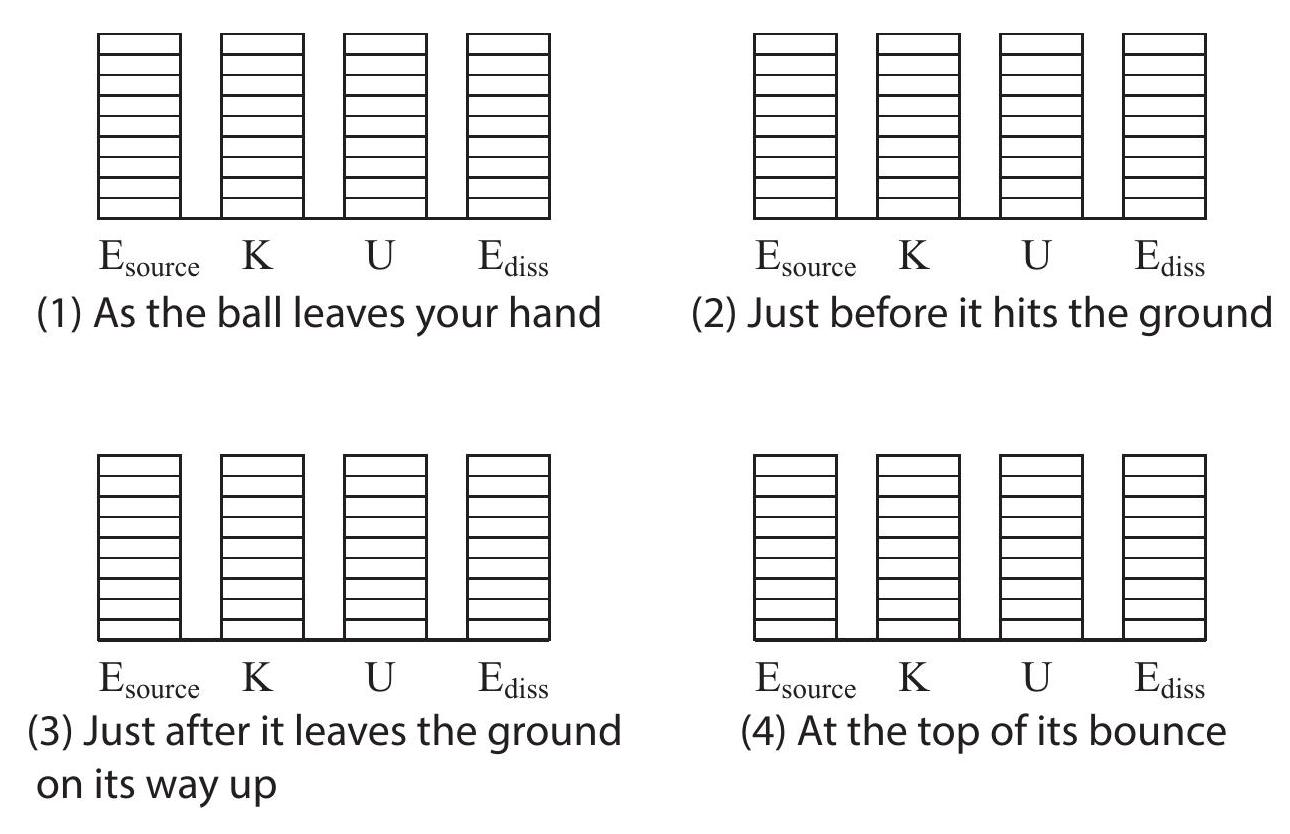
\includegraphics[max width=\textwidth]{2024_09_14_9969b06773f10b6936e8g-128}
\end{center}

\section*{Problem 4}
A $60-\mathrm{kg}$ skydiver jumps from an airplane 4000 m above the earth. After falling 450 m , he reaches a terminal speed of $55 \mathrm{~m} / \mathrm{s}$ (about 120 mph ). This means that after this time his speed does not increase any more.\\
(a) At the moment of the jump, what is the initial (gravitational) potential energy of the system formed by the earth and the skydiver? (Take $U^{G}=0$ at ground level.)\\
(b) After the skydiver has fallen 450 m , what is the (gravitational) potential energy of the system? (Call this the "final" potential energy.)\\
(c) What is the final kinetic energy of the diver at that time?\\
(d) Assume the initial kinetic energy of the skydiver is zero. Is $\Delta K=-\Delta U$ for this system? If not, explain what happened to the "missing" energy.\\
(e) Can the skydiver and the earth below (excluding the atmosphere!) be considered a closed system\\
here? Explain.\\
(f) After the skydiver reaches terminal speed (and before he opens his parachute), he falls for a while at constant speed. What kind of energy conversion is taking place during this time? (Consider the system to be the earth, the skydiver, and the air around him).

\section*{Problem 5}
You shoot a 1-kg projectile straight up from a spring toy gun, and find that it reaches a height of 5 m . (How do you figure out the height? From the time of flight, of course! See problem 2 from Chapter 2.) You also measure that when you load the gun, the spring compresses a distance 10 cm . What is the value of the spring constant?

\section*{Chapter 6}
\section*{Interactions, part 2: Forces}
\subsection*{6.1 Force}
As we saw in the previous chapter, when an interaction can be described by a potential energy function, it is possible to use this to get a full solution for the motion of the objects involved, at least in one dimension. In fact, energy-based methods (known as the Lagrangian and Hamiltonian methods) can be also generalized to deal with problems in three dimensions, and they also provide the most direct pathway to quantum mechanics and quantum field theory. It might be possible to write an advanced textbook on classical mechanics without mentioning the concept of force at all.

On the other hand, as you may have also gathered from the example I worked out at the end of the previous chapter (section 5.6.3), solving for the equation of motion using energy-based methods may involve somewhat advanced math, even in just one dimension, and it only gets more complicated in higher dimensions. There is also the question of how to deal with interactions that are not conservative (at the macroscopic level) and therefore cannot be described by a potential energy function of the macroscopic coordinates. And, finally, there are specialized problem areas (such as the entire field of statics) where you actually want to know the forces acting on the various objects involved. For all these reasons, the concept of force will be introduced here, and the next few chapters will illustrate how it may be used to solve a variety of elementary problems in classical mechanics. This does not mean, however, that we are going to forget about energy from now on: as we will see, energy methods will continue to provide useful shortcuts in a variety of situations as well.

We start, as usual, by considering two objects that form an isolated system, so they interact with each other and with nothing else. As we have seen, under these circumstances their individual momenta change, but the total momentum remains constant. We are going to take the rate of\\
change of each object's momentum as a measure of the force exerted on it by the other object. Mathematically, this means we will write for the average force exerted by 1 on 2 over the time interval $\Delta t$ the expression


\begin{equation*}
\left(F_{12}\right)_{a v}=\frac{\Delta p_{2}}{\Delta t} \tag{6.1}
\end{equation*}


Please observe the notation we are going to use: the subscripts on the symbol $F$ are in the order "by,on", as in "force exerted by" (object identified by first subscript) "on" (object identified by second subscript). (The comma is more or less optional.)

You can also see from Eq. (6.1) that the SI units of force are $\mathrm{kg} \cdot \mathrm{m} / \mathrm{s}^{2}$. This combination of units has the special name "newton," and it's abbreviated by an uppercase N.

In the same way as above, we can write the average force exerted by object 2 on object 1 :


\begin{equation*}
\left(F_{21}\right)_{a v}=\frac{\Delta p_{1}}{\Delta t} \tag{6.2}
\end{equation*}


and we know, by conservation of momentum, that we must have $\Delta p_{1}=-\Delta p_{2}$, so we get our first important result,


\begin{equation*}
\left(F_{12}\right)_{a v}=-\left(F_{21}\right)_{a v} \tag{6.3}
\end{equation*}


That is, whenever two objects interact, they always exert equal (in magnitude) and opposite (in direction) forces on each other. This is most often called Newton's third law of motion, or informally "the law of action and reaction."

We might as well now proceed along familiar lines and take the limit of Eqs. (6.1) and (6.2) above, as $\Delta t$ goes to zero, in order to introduce the more general concept of the instantaneous force (or just the "force," without any further qualifiers). We then get


\begin{align*}
& F_{12}=\frac{d p_{2}}{d t} \\
& F_{21}=\frac{d p_{1}}{d t} \tag{6.4}
\end{align*}


and, since Eq. (6.3) should hold for a time interval of any size,


\begin{equation*}
F_{12}=-F_{21} \tag{6.5}
\end{equation*}


Now, under most circumstances the mass of, say, object 2 will not change during the interaction, so we can write


\begin{equation*}
F_{12}=\frac{d}{d t}\left(m_{2} v_{2}\right)=m_{2} \frac{d v_{2}}{d t}=m_{2} a_{2} \tag{6.6}
\end{equation*}


This is the result that we often refer to as " $F=m a$ ", also known as Newton's second law of motion: the (net) force acting on an object is equal to the product of its inertial mass and its acceleration. The formulation in terms of the rate of change of momentum, as in Eqs. (6.4), is,\\
however, somewhat more general, so it is technically preferred, even though this semester we will directly use $F=m a$ throughout.

If you want an example of a physical situation where $F=d p / d t$ is not equivalent to $F=m a$, consider a system where object 1 is a rocket, including its fuel, and "object" 2 are the gases ejected by the rocket. In this case, the mass of both "objects" is constantly changing, as the fuel is burned and more gases are ejected, and so the more general form $F=d p / d t$ needs to be used to calculate the force on the rocket (the thrust) at any given time.

At this point you may be wondering just what is Newton's first law? It is just the law of inertia: an object on which no force acts will stay at rest if it is initially at rest, or will move with constant velocity.

\subsection*{6.1.1 Forces and systems of particles}
What if you had, say, three objects (let us make them "particles," for simplicity), all interacting with one another? In physics we find that all our interactions are pairwise additive, that is, we can write the total potential energy of the system as the sum of the potential energies associated with each pair of particles separately. As we will see in a moment, this means that the corresponding forces are additive too, so that, for instance, the total force on particle 1 could be written as


\begin{equation*}
F_{\text {all }, 1}=F_{21}+F_{31}=\frac{d p_{1}}{d t} \tag{6.7}
\end{equation*}


Consider now the most general case of a system that has an arbitrary number of particles, and is not isolated; that is, there are other objects, outside the system, that exert forces on some or all of the particles that make up the system. We will call these external forces. The sum of all the forces (both internal and external) acting on all the particles will take a form like this:


\begin{equation*}
F_{\text {total }}=F_{\text {ext }, 1}+F_{21}+F_{31}+\ldots+F_{e x t, 2}+F_{12}+F_{32}+\ldots+\ldots=\frac{d p_{1}}{d t}+\frac{d p_{2}}{d t}+\ldots \tag{6.8}
\end{equation*}


where $F_{\text {ext }, 1}$ is the sum of all the external forces acting on particle 1, and so on. But now, observe that because of Newton's third law, Eq. (6.5), for every term of the form $F_{i j}$ appearing in the sum (6.8), there is a corresponding term $F_{j i}=-F_{i j}$ (you can see this explicitly already in Eq. (6.8) with $F_{12}$ and $F_{21}$ ), so all those terms (which represent all the internal forces) are going to cancel out, and we will be left only with the sum of the external forces:


\begin{equation*}
F_{e x t, 1}+F_{e x t, 2}+\ldots=\frac{d p_{1}}{d t}+\frac{d p_{2}}{d t}+\ldots \tag{6.9}
\end{equation*}


The left-hand side of this equation is the sum of all the external forces; the right-hand side is the rate of change of the total momentum of the system. But the total momentum of the system is\\
just equal to $M v_{c m}$ (compare Eq. (3.11), in the "Momentum" chapter). So we have


\begin{equation*}
F_{\text {ext }, a l l}=\frac{d p_{\text {sys }}}{d t}=\frac{d}{d t}\left(M v_{c m}\right) \tag{6.10}
\end{equation*}


This extends a previous result. We already knew that in the absence of external forces, the momentum of a system remained constant. Now we see that the system's momentum responds to the net external force as if the whole system was a single particle of mass equal to the total mass $M$ and moving at the center of mass velocity $v_{c m}$. In fact, assuming that $M$ does not change we can rewrite Eq. (6.10) in the form


\begin{equation*}
F_{\text {ext,all }}=M a_{c m} \tag{6.11}
\end{equation*}


where $a_{c m}$ is the acceleration of the center of mass. This is the key result that allows us to treat extended objects as if they were particles: as far as the motion of the center of mass is concerned, all the internal forces cancel out (as we already saw in our study of collisions), and the point representing the center of mass responds to the sum of the external forces as if it were just a particle of mass $M$ subject to Newton's second law, $F=m a$. The result (6.11) applies equally well to an extended solid object that we choose to mentally break up into a collection of particles, as to an actual collection of separate particles, or even to a collection of separate extended objects; in the latter case, we would just have each object's motion represented by the motion of its own center of mass.

Finally, note that all the results above generalize to more than one dimension. In fact, forces are vectors (just like velocity, acceleration and momentum), and all of the above equations, in 3 dimensions, apply separately to each vector component. In one dimension, we just need to be aware of the sign of the forces, whenever we add several of them together.

\subsection*{6.2 Forces and potential energy}
In the last chapter I mentioned a special case that we encounter often, in which a lighter object is interacting with a much more massive one, so that the massive one essentially does not move at all as a result of the interaction. Note that this does not contradict Newton's 3rd law, Eq. (6.5): the forces the two objects exert on each other are the same in magnitude, but the acceleration of each object is inversely proportional to its mass, so $F_{12}=-F_{21}$ implies


\begin{equation*}
m_{2} a_{2}=-m_{1} a_{1} \tag{6.12}
\end{equation*}


and so if, for instance, $m_{2} \gg m_{1}$, we get $\left|a_{2}\right|=\left|a_{1}\right| m_{1} / m_{2} \ll\left|a_{1}\right|$. In words, the more massive object is less responsive than the less massive one to a force of the same magnitude. This is just how we came up with the concept of inertial mass in the first place!

Anyway, you'll recall that in this situation I could just write the potential energy function of the whole system as a function of only the lighter object's coordinate, $U(x)$. I am going to use this\\
simplified setup to show you a very interesting relationship between potential energies and forces. Suppose this is a closed system in which no dissipation of energy is taking place. Then the total mechanical energy is a constant:


\begin{equation*}
E_{\text {mech }}=\frac{1}{2} m v^{2}+U(x)=\text { constant } \tag{6.13}
\end{equation*}


(Here, $m$ is the mass of the lighter object, and $v$ its velocity; the more massive object does not contribute to the total kinetic energy, since it does not move!)

As the lighter object moves, both $x$ and $v$ in Eq. (6.13) change with time (recall, for instance, our study of "energy landscapes" in the previous chapter, section 5.1.2). So I can take the derivative of Eq. (6.13) with respect to time, using the chain rule, and noting that, since the whole thing is a constant, the total value of the derivative must be zero:


\begin{align*}
0 & =\frac{d}{d t}\left(\frac{1}{2} m(v(t))^{2}+U(x(t))\right) \\
& =m v(t) \frac{d v}{d t}+\frac{d U}{d x} \frac{d x}{d t} \tag{6.14}
\end{align*}


But note that $d x / d t$ is just the same as $v(t)$. So I can cancel that on both terms, and then I am left with


\begin{equation*}
m \frac{d v}{d t}=-\frac{d U}{d x} \tag{6.15}
\end{equation*}


But $d v / d t$ is just the acceleration $a$, and $F=m a$. So this tells me that


\begin{equation*}
F=-\frac{d U}{d x} \tag{6.16}
\end{equation*}


and this is how you can always get the force from a potential energy function.\\
Let us check it right away for the force of gravity: we know that $U^{G}=m g y$, so


\begin{equation*}
F^{G}=-\frac{d U^{G}}{d y}=-\frac{d}{d y}(m g y)=-m g \tag{6.17}
\end{equation*}


Is this right? It seems to be! Recall all objects fall with the same acceleration, $-g$ (assuming the upwards direction to be positive), so if $F=m a$, we must have $F^{G}=-m g$. So the gravitational force exerted by the earth on any object (which I would denote in full by $F_{E, o}^{G}$ ) is proportional to the inertial mass of the object - in fact, it is what we call the object's weight - but since to get the acceleration you have to divide the force by the inertial mass, that cancels out, and $a$ ends up being the same for all objects, regardless of how heavy they are.

Now that we have this result under our belt, we can move on to the slightly more challenging case of two objects of comparable masses interacting through a potential energy function that must be, as I pointed out in the previous chapter, a function of just the relative coordinate $x_{12}=x_{2}-x_{!}$.

I claim that in that case you can again get the force on object $1, F_{21}$, by taking the derivative of $U\left(x_{2}-x_{1}\right)$ with respect to $x_{1}$ (leaving $x_{2}$ alone), and reciprocally, you get $F_{12}$ by taking the derivative of $U\left(x_{2}-x_{1}\right)$ with respect to $x_{2}$. Here is how it works, again using the chain rule:


\begin{align*}
& F_{21}=-\frac{d}{d x_{1}} U\left(x_{12}\right)=-\frac{d U}{d x_{12}} \frac{d}{d x_{1}}\left(x_{2}-x_{1}\right)=\frac{d U}{d x_{12}} \\
& F_{12}=-\frac{d}{d x_{2}} U\left(x_{12}\right)=-\frac{d U}{d x_{12}} \frac{d}{d x_{2}}\left(x_{2}-x_{1}\right)=-\frac{d U}{d x_{12}} \tag{6.18}
\end{align*}


and you can see that this automatically ensures that $F_{21}=-F_{12}$. In fact, it was in order to ensure this that I required that $U$ should depend only on the difference of $x_{1}$ and $x_{2}$, rather than on each one separately. Since we got the condition $F_{21}=-F_{12}$ originally from conservation of momentum, you can see now how the two things are related ${ }^{1}$.

The only example we have seen so far of this kind of potential energy function was in last chapter's Section 5.1.1, for two carts interacting through an "ideal" spring. I told you there that the potential energy of the system could be written as $\frac{1}{2} k\left(x_{2}-x_{1}-x_{0}\right)^{2}$, where $k$ was the "spring constant" and $x_{0}$ the relaxed length of the spring. If you apply Eqs. (6.18) to this function, you will find that the force exerted (through the spring) by cart 2 on cart 1 is


\begin{equation*}
F_{21}=k\left(x_{2}-x_{1}-x_{0}\right) \tag{6.19}
\end{equation*}


Note that this force will be negative under the assumptions we made last chapter, namely, that cart 2 is on the right, cart 1 on the left, and the spring is compressed, so that $x_{2}-x_{1}<x_{0}$. Similarly,


\begin{equation*}
F_{12}=-k\left(x_{2}-x_{1}-x_{0}\right) \tag{6.20}
\end{equation*}


and this one, as it should, is positive.\\
The results (6.19) and (6.20) basically tell you what we mean by an "ideal spring" in physics: it is a spring that pulls (if stretched) or pushes (if compressed) with a force that is proportional to the change from its equilibrium length. Thus, if you fasten one end of the spring at $x=0$, and stretch it or compress it so that the other end is at $x$, the spring will respond by exerting a force


\begin{equation*}
F^{s p r}=-k\left(x-x_{0}\right) \tag{6.21}
\end{equation*}


As you can see, this is negative if $x>x_{0}>0$ (spring stretched, pulling force) and positive if $x<x_{0}$ (spring compressed, pushing force). In fact, the spring exerts an equal (in magnitude) and opposite (in direction) force at the other end (the one attached to the wall), so Eq. (6.21) only gives the correct sign of the force at the end that is denoted by the coordinate value $x$. Equations (6.19) and (6.20) are a bit clearer in this respect: Eq. (6.19) gives the correct sign of the force at point $x_{1}$, and Eq. (6.20) the correct sign at point $x_{2}$.

\footnotetext{${ }^{1}$ The result (6.18) generalizes to more dimensions, but to do it properly you need vectors and partial derivative notation, and I'm already bending the notational rules a little bit here...
}Figure 6.1 shows, in black, all the forces exerted by a spring with one fixed end, according as to whether it is relaxed, compressed, or stretched. I have assumed that it is pushed or pulled by a hand (not shown) at the "free" end, hence the subscript " $h$ ", whereas the subscript " $w$ " stands for "wall." Note that the wall and the hand, in turn, exert equal and opposite forces on the spring, shown in red in the figure.

\begin{center}
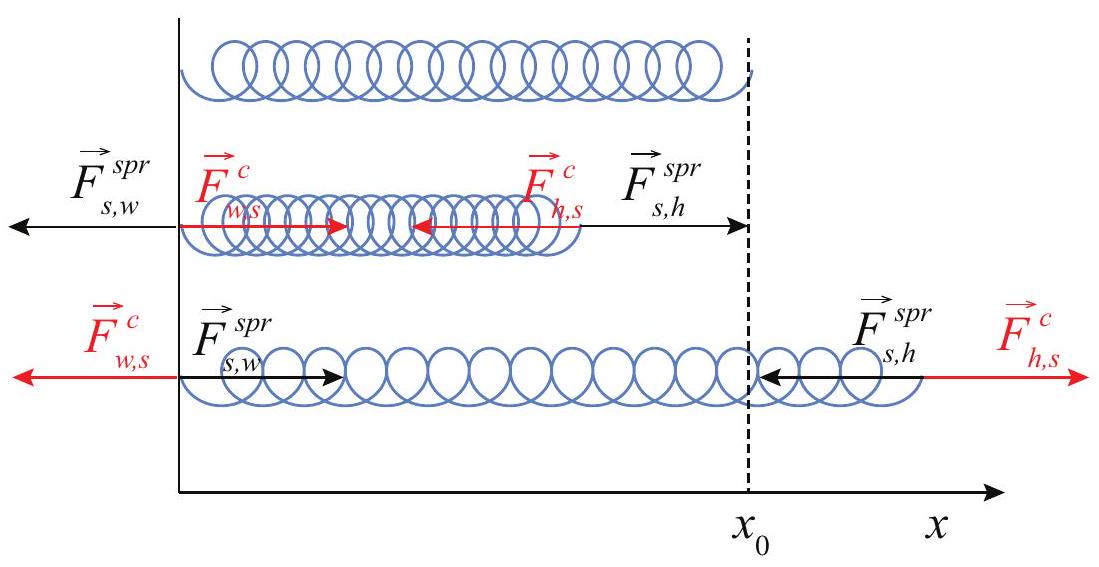
\includegraphics[max width=\textwidth]{2024_09_14_9969b06773f10b6936e8g-137}
\end{center}

Figure 6.1: Forces (in black) exerted by a spring with one end attached to a wall and the other pushed or pulled by a hand (not shown). In every case the force is proportional to the change in the length of the spring from its equilibrium, or relaxed, value, shown here as $x_{0}$. For this figure I have set the proportionality constant $k=1$. The forces exerted on the spring, by the wall and by the hand, are shown in red.

Equation (6.21) is generally referred to as Hooke's law, after the British scientist Robert Hooke (a contemporary of Newton). Of course, it is not a "law" at all, merely a useful approximation to the way most springs behave as long as you do not stretch them or compress them too much ${ }^{2}$.

A note on the way the forces have been labeled in Figure 6.1. I have used the generic symbol " $c$ ", which stands for "contact," to indicate the type of force exerted by the wall and the hand on the spring. In fact, since each pair of forces (by the hand on the spring and by the spring on the hand, for instance), at the point of contact, arises from one and the same interaction, I should have used the same "type" notation for both, but it is widespread practice to use a superscript like "spr" to denote a force whose origin is, ultimately, a spring's elasticity. This does not change the fact that the spring force, at the point where it is applied, is indeed a contact force.

So, next, a word on "contact" forces. Basically, what we mean by that is forces that arise where objects "touch," and we mean this by opposition to what are called instead "field" forces (such as gravity, or magnetic or electrostatic forces) which "act at a distance." The distinction is actually

\footnotetext{${ }^{2}$ Assuming that you can compress them! Some springs, such as slinkies, actually cannot be compressed because their coils are already in contact when they are relaxed. Nevertheless, Eq. (6.21) will still apply approximately to such a spring when it is stretched, that is, when $x>x_{0}$.
}
only meaningful at the macroscopic level, since at the microscopic level objects never really touch, and all forces are field forces, it is just that some are "long range" and some are "short range." For our purposes, really, the word "contact" will just be a convenient, catch-all sort of moniker that we will use to label the force vectors when nothing more specific will do.

\subsection*{6.3 Forces not derived from a potential energy}
As we have seen in the previous section, for interactions that are associated with a potential energy, we are always able to determine the forces from the potential energy by simple differentiation. This means that we do not have to rely exclusively on an equation of the type $F=m a$, like (6.4) or (6.6), to infer the value of a force from the observed acceleration; rather, we can work in reverse, and predict the value of the acceleration (and from it all the subsequent motion) from our knowledge of the force.

I have said before that, on a microscopic level, all the interactions can be derived from potential energies, yet at the macroscopic level this is not generally true: we have many kinds of interactions for which the associated "stored" or converted energy cannot, in general, be written as a function of the macroscopic position variables for the objects making up the system (by which I mean, typically, the positions of their centers of mass). So what do we do in those cases?

The forces of this type with which we shall deal this semester actually fall into two different categories: the ones that do not dissipate energy, and that we could, in fact, associate with a potential energy if we wanted to ${ }^{3}$, and the ones that definitely dissipate energy and need special handling. The former category includes the normal force, tension, and the static friction force; the second category includes the force of kinetic (or sliding) friction, and air resistance. A brief description of all these forces, and the methods to deal with them, follows.

\subsection*{6.3.1 Tensions}
Tension is the force exerted by a stretched spring, and, similarly, by objects such as cables, ropes, and strings in response to a stretching force (or load) applied to them. It is ultimately an elastic force, so, as I said above, we could in principle describe it by a potential energy, but in practice cables, strings and the like are so stiff that it is often all right to neglect their change in length altogether and assume that no potential energy is, in fact, stored in them. The price we pay for this simplification (and it is a simplification) is that we are left without an independent way to determine the value of the tension in any specific case; we just have to infer it from the acceleration

\footnotetext{${ }^{3}$ If we wanted to complicate our life, that is...
}
of the object on which it acts (since it is a reaction force, it can assume any value as required to adjust to any circumstance - up to the point where the rope snaps, anyway).

Thus, for instance, in the picture below, which shows two blocks connected by a rope over a pulley, the tension force exerted by the rope on block 1 must equal $m_{1} a_{1}$, where $a_{1}$ is the acceleration of that block, provided there are no other horizontal forces (such as friction) acting on it. For the hanging block, on the other hand, the net force is the sum of the tension on the other end of the rope (pulling up) and gravity, pulling down. If we choose the upward direction as positive, we can write Newton's second law for the second block as


\begin{equation*}
F_{r, 2}^{t}-m_{2} g=m_{2} a_{2} \tag{6.22}
\end{equation*}


Two things need to be realized now. First, if the rope is inextensible, both blocks travel the same distance in the same time, so their speeds are always the same, and hence the magnitude of their accelerations will always be the same as well; only the sign may be different depending on which direction we choose as positive. If we take to the right to be positive for the horizontal motion, we will have $a_{2}=-a_{1}$. I'm just going to call $a_{1}=a$, so then $a_{2}=-a$.

\begin{center}
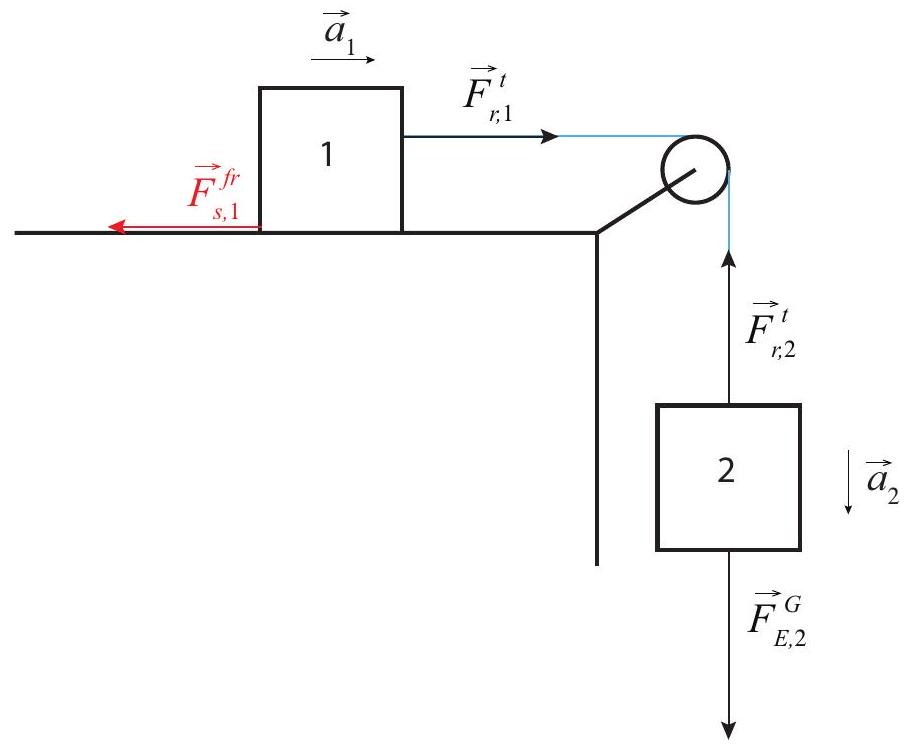
\includegraphics[max width=\textwidth]{2024_09_14_9969b06773f10b6936e8g-139}
\end{center}

Figure 6.2: Two blocks joined by a massless, inextensible strength threaded over a massless pulley. An optional friction force (in red, where $f r$ could be either $s$ or $k$ ) is shown for use later, in the discussion in subsection 3.3. In this subsection, however, it is assumed to be zero.

The second thing to note is that, if the rope's mass is negligible, it will, like an ideal spring, pull with a force with the same magnitude on both ends. With our specific choices (up and to the right is positive), we then have $F_{r, 2}^{t}=F_{r, 1}^{t}$, and I'm just going to call this quantity $F^{t}$. All this yields,\\
then, the following two equations:


\begin{align*}
F^{t} & =m_{1} a \\
F^{t}-m_{2} g & =-m_{2} a \tag{6.23}
\end{align*}


The system (6.23) can be easily solved to get


\begin{align*}
a & =\frac{m_{2} g}{m_{1}+m_{2}} \\
F^{t} & =\frac{m_{1} m_{2} g}{m_{1}+m_{2}} \tag{6.24}
\end{align*}


\subsection*{6.3.2 Normal forces}
Normal force is the reaction force with which a surface pushes back when it is being pushed on. Again, this works very much like an extremely stiff spring, this time under compression instead of tension. And, again, we will eschew the potential energy treatment by assuming that the surface's actual displacement is entirely negligible, and we will just calculate the value of $F^{n}$ as whatever is needed in order to make Newton's second law work. Note that this force will always be perpendicular to the surface, by definition (the word "normal" means "perpendicular" here); the task of dealing with a sideways push on the surface will be delegated to the static friction force, to be covered next.

If I am just standing on the floor and not falling through it, the net vertical force acting on me must be zero. The force of gravity on me is $m g$ downwards, and so the upwards normal force must match this value, so for this situation $F^{n}=m g$. But don't get too attached to the notion that the normal force must always be equal to $m g$, since this will often not be the case. Imagine, for instance, a person standing inside an elevator at the time it is accelerating upwards. With the upwards direction as positive, Newton's second law for the person reads


\begin{equation*}
F^{n}-m g=m a \tag{6.25}
\end{equation*}


and therefore for this situation


\begin{equation*}
F^{n}=m g+m a \tag{6.26}
\end{equation*}


If you were weighing yourself on a bathroom scale in the elevator, this is the upwards force that the bathroom scale would have to exert on you, and it would do that by compressing a spring inside, and it would record the "extra" compression (beyond that required by your actual weight, mg ) as extra weight. Conversely, if the elevator were accelerating downward, the scale would record you as being lighter. In the extreme case in which the cable of the elevator broke and you, the elevator and the scale ended up (briefly, before the emergency brake caught on) in free fall, you would all be falling with the same acceleration, you would not be pushing down on the scale at all, and its normal force as well as your recorded weight would be zero. This is ultimately the reason\\
for the apparent weightlessness experienced by the astronauts in the space station, where the force of gravity is, in fact, not very much smaller than on the surface of the earth. (We will return to this effect after we have a good grip on two-dimensional, and in particular circular, motion.)

\subsection*{6.3.3 Static and kinetic friction forces}
The static friction force is a force that prevents two surfaces in contact from slipping relative to each other. It is an extremely useful force, since we would not be able to drive a car, or ride a bicycle, or even walk, without it - as we know from experience, if we have ever tried to do any of those things on a low-friction surface (such as a sheet of ice).

The science behind friction (known technically as tribology) is actually not very simple at all, and it is of great current interest for many reasons-whether the ultimate goal is to develop ways to reduce friction or to increase it. On an elementary level, we are all aware of the fact that even a surface that looks smooth on a macroscopic scale will actually exhibit irregularities, such as ridges and valleys, under a microscope. It makes sense, then, that when two such surfaces are pressed together, the bumps on one of them will hit, and be held in place by, the bumps on the other one, and that will prevent sliding until and unless a sufficient force is applied to temporarily "flatten" the bumps enough to allow the thing to move ${ }^{4}$.

As long as this does not happen, that is, as long as the surfaces do not slide relative to each other, we say we are dealing with the static friction force, which is, at least approximately, an elastic force that does not dissipate energy: the small distortion of the "bumps" on the surfaces that takes place when you push on them typically happens slowly enough, and is small enough, to be reversible, so that when you stop pushing the two surfaces just go back to their initial state. This is no longer the case once the surfaces start sliding relative to each other. At that point the character of the friction force changes, and we have to deal with the sliding, or kinetic friction force, as I will explain below.

The static friction force is also, like tension and the normal force, a reaction force that will adjust itself, within limits, to take any value required to prevent slippage in a given circumstance. Hence, its actual value in a particular situation cannot really be ascertained until the other relevant forcesthe other forces pushing or pulling on the object-are known.

For instance, for the system in Figure 6.2, imagine there is a force of static friction between block 1 and the surface on which it rests, sufficiently large to keep it from sliding altogether. How large

\footnotetext{${ }^{4}$ This picture based, essentially, on classical physics, leaves out an atomic-scale effect that may be important in some cases, which is the formation of weak bonds between the atoms of both surfaces, resulting in an actual "adhesive" force. This is, for instance, how geckos can run up vertical walls. For our purposes, however, the classical picture (of small ridges and valleys bumping into each other) will suffice to qualitatively understand all the examples we will cover this semester.
}
does this have to be? If there is no acceleration $(a=0)$, the equivalent of system (6.23) will be\\
\$\$

\begin{align*}
F_{s, 1}^{s}+F^{t} & =0 \\
F^{t}-m_{2} g & =0 \tag{6.27}
\end{align*}


where $F_{s, 1}^{s}$ is the force of static friction exerted by the surface on block 1 , and we are going to let the math tell us what sign it is supposed to have. Solving the system (6.27) we just get the condition


\begin{equation*}
F_{s, 1}^{s}=-m_{2} g \tag{6.28}
\end{equation*}


so this is how large $F_{s, 1}^{s}$ has to be in order to keep the whole system from moving in this case.
There is an empirical formula that tells us approximately how large the force of static friction can get in a given situation. The idea behind it is that, microscopically, the surfaces are in contact only near the top of their respective ridges. If you press them together harder, some of the ridges get flattened and the effective contact area increases; this in turn makes the surfaces more resistant to slippage. A direct measure of how strongly the two surfaces press against each other is, actually, just the normal force they exert on each other. So, in general, we expect the maximum force that static friction will be able to exert to be proportional to the normal force between the surfaces:


\begin{equation*}
\left|F_{s 1, s 2}^{s}\right|_{\max }=\mu_{s}\left|F_{s 1, s 2}^{n}\right| \tag{6.29}
\end{equation*}


where $s 1$ and $s 2$ just mean "surface 1 " and "surface 2," respectively, and the number $\mu_{s}$ is known as the coefficient of static friction: it is a tabulated quantity that is determined experimentally, by testing the slippage of different surfaces against each other under different loads.

In our example, the normal force exerted by the surface on block 1 has to be equal to $m_{1} g$, since there is no vertical acceleration for that block, and so the maximum value that $F^{s}$ may have in this case is $\mu_{s} m_{1} g$, whatever $\mu_{s}$ might happen to be. In fact, this setup would give us a way to determine $\mu_{s}$ for these two surfaces: start with a small value of $m_{2}$, and gradually increase it until the system starts moving. At that point we will know that $m_{2} g$ has just exceeded the maximum possible value of $\left|F_{12}^{s}\right|$, namely, $\mu_{s} m_{1} g$, and so $\mu_{s}=\left(m_{2}\right)_{\max } / m_{1}$, where $\left(m_{2}\right)_{\max }$ is the largest mass we can hang before the system starts moving.

By contrast with all of the above, the kinetic friction force, which always acts so as to oppose the relative motion of the two surfaces when they are actually slipping, is not elastic, it is definitely dissipative, and, most interestingly, it is also not much of a reactive force, meaning that its value can be approximately predicted for any given circumstance, and does not depend much on things such as how fast the surfaces are actually moving relative to each other. It does depend on how hard the surfaces are pressing against each other, as quantified by the normal force, and on another tabulated quantity known as the coefficient of kinetic friction:


\begin{equation*}
\left|F_{s 1, s 2}^{k}\right|=\mu_{k}\left|F_{s 1, s 2}^{n}\right| \tag{6.30}
\end{equation*}


Note that, unlike for static friction, this is not the maximum possible value of $\left|F^{k}\right|$, but its actual value; so if we know $F^{n}$ (and $\mu_{k}$ ) we know $F^{k}$ without having to solve any other equations (its sign does depend on the direction of motion, of course). The coefficient $\mu_{k}$ is typically a little smaller than $\mu_{s}$, reflecting the fact that once you get something you have been pushing on to move, keeping it in motion with constant velocity usually does not require the same amount of force.

To finish off with our example in Figure 2, suppose the system is moving, and there is a kinetic friction force $F_{s, 1}^{k}$ between block 1 and the surface. The equations (6.23) then have to be changed to


\begin{align*}
F^{t}-\mu_{k} m_{1} g & =m_{1} a \\
F^{t}-m_{2} g & =-m_{2} a \tag{6.31}
\end{align*}


and the solution now is


\begin{align*}
a & =\frac{m_{2}-\mu_{k} m_{1}}{m_{1}+m_{2}} g \\
F^{t} & =\frac{m_{1} m_{2}\left(1+\mu_{k}\right)}{m_{1}+m_{2}} g \tag{6.32}
\end{align*}


You may ask, why does kinetic friction dissipate energy? A qualitative answer is that, as the surfaces slide past each other, their small (sometimes microscopic) ridges are constantly "bumping" into each other; so you have lots of microscopic collisions happening all the time, and they cannot all be perfectly elastic. So mechanical energy is being "lost." In fact, it is primarily being converted to thermal energy, as you can verify experimentally: this is why you rub your hands together to get warm, for instance. More dramatically, this is how some people (those who really know what they are doing!) can actually start a fire by rubbing sticks together.

\subsection*{6.3.4 Air resistance}
Air resistance is an instance of fluid resistance or drag, a force that opposes the motion of an object through a fluid. Microscopically, you can think of it as being due to the constant collisions of the object with the air molecules, as it cleaves its way through the air. As a result of these collisions, some of its momentum is transferred to the air, as well as some of its kinetic energy, which ends up as thermal energy (as in the case of kinetic friction discussed above). The very high temperatures that air resistance can generate can be seen, in a particularly dramatic way, on the re-entry of spacecraft into the atmosphere.

Unlike kinetic friction between solid surfaces, the fluid drag force does depend on the velocity of the object (relative to the fluid), as well as on a number of other factors having to do with the object's shape and the fluid's density and viscosity. Very roughly speaking, for low velocities the\\
drag force is proportional to the object's speed, whereas for high velocities it is proportional to the square of the speed.

In principle, one can use the appropriate drag formula together with Newton's second law to calculate the effect of air resistance on a simple object thrown or dropped; in practice, this requires a somewhat more advanced math than we will be using this course, and the formulas themselves are complicated, so I will not introduce them here.

One aspect of air resistance that deserves to be mentioned is what is known as "terminal velocity" (which I already introduced briefly in Section 2.3). Since air resistance increases with speed, if you drop an object from a sufficiently great height, the upwards drag force on it will increase as it accelerates, until at some point it will become as large as the downward force of gravity. At that point, the net force on the object is zero, so it stops accelerating, and from that point on it continues to fall with constant velocity. When the Greek philosopher Aristotle was trying to figure out the motion of falling bodies, he reasoned that, since air was just another fluid, he could slow down the fall (in order to study it better) without changing the physics by dropping objects in liquids instead of air. The problem with this approach, though, is that terminal velocity is reached much faster in a liquid than in air, so Aristotle missed entirely the early stage of approximately constant acceleration, and concluded (wrongly) that the natural way all objects fell was with constant velocity. It took almost two thousand years until Galileo disproved that notion by coming up with a better method to slow down the falling motion-namely, by using inclined planes.

\subsection*{6.4 Free-body diagrams}
As Figure 6.1 shows, trying to draw every single force acting on every single object can very quickly become pretty messy. And anyway, this is not usually what we need: what we need is to separate cleanly all the forces acting on any given object, one object at a time, so we can apply Newton's second law, $F_{n e t}=m a$, to each object individually.

In order to accomplish this, we use what are known as free-body diagrams. In a free-body diagram, a potentially very complicated object is replaced symbolically by a dot or a small circle, and all the forces acting on the object are drawn (approximately to scale and properly labeled) as acting on the dot. Regardless of whether a force is a pulling or pushing force, the convention is to always draw it as a vector that originates at the dot. If the system is accelerating, it is also a good idea to indicate the acceleration's direction also somewhere on the diagram.

The figure below (next page) shows, as an example, a free-body diagram for block 1 in Figure 6.2, in the presence of both a nonzero acceleration and a kinetic friction force. The diagram includes all the forces, even gravity and the normal force, which were left out of the picture in Figure 6.2.

\begin{center}
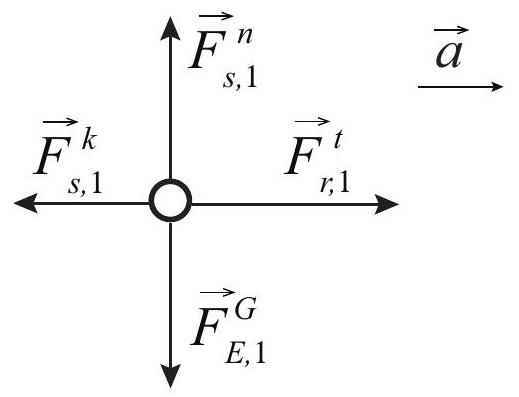
\includegraphics[max width=\textwidth]{2024_09_14_9969b06773f10b6936e8g-145}
\end{center}

Figure 6.3: Free-body diagram for block 1 in Figure 6.2, with the friction force adjusted so as to be compatible with a nonzero acceleration to the right.

Note that I have drawn $F^{n}$ and the force of gravity $F_{E, 1}^{G}$ as having the same magnitude, since there is no vertical acceleration for that block. If I know the value of $\mu_{k}$, I should also try to draw $F^{k}=\mu_{k} F^{n}$ approximately to scale with the other two forces. Then, since I know that there is an acceleration to the right, I need to draw $F^{t}$ greater than $F^{k}$, since the net force on the block must be to the right as well. And, if I were drawing a free-body diagram for block 2, I would have to make sure that I drew its weight, $F_{E, 2}^{G}$, as being greater in magnitude than $F^{t}$, since the net force on that block needs to be downwards.

\subsection*{6.5 In summary}
\begin{enumerate}
  \item Whenever two objects interact, they exert forces on each other that are equal in magnitude and opposite in direction (Newton's 3rd law).
  \item Forces are vectors, and they are additive. The total (or net) force on an object or system is equal to the rate of change of its total momentum (Newton's 2nd law). If the system's mass is constant, this can be written as $F_{\text {ext,all }}=M a_{c m}$, where $M$ is the system's total mass and $a_{c m}$ is the acceleration of its center of mass. Only the external forces contribute to this equation; the internal forces cancel out because of point 1 above.
  \item For any interaction that can be derived from a potential energy function $U\left(x_{1}-x_{2}\right)$, the force exerted by object 2 on object 1 is equal to $-d U / d x_{1}$ (where the derivative is calculated treating $x_{2}$ as a constant), and vice-versa.
  \item The force of gravity on an object near the surface of the earth is known as the object's weight, and it is equal (in magnitude) to $m g$, where $m$ is the object's inertial mass.
  \item An ideal spring whose relaxed length is $x_{0}$, when stretched or compressed to a length $x$, exerts a pulling or pushing force, respectively, at both ends, with magnitude $k\left|x-x_{0}\right|$, where $k$ is called the spring constant.
  \item When dealing with macroscopic objects we introduce several "constraint" forces whose values need to be determined from the accelerations through Newton's second law: the tension $F^{t}$ in ropes, strings or cables; the normal force $F^{n}$ exerted by a surface in response to applied pressure; and the static friction force $F^{s}$ that prevents surfaces from slipping past each other.
  \item The maximum possible value of the static friction force is $\mu_{s}\left|F^{n}\right|$, where $\mu_{s}$ is the coefficient of static friction.
  \item The force of sliding or kinetic friction, $F^{k}$, appears when two surfaces are sliding past each other. Its magnitude is $\mu_{k}\left|F^{n}\right|$ ( $\mu_{k}$ is the coefficient of static friction), and its sign is such as to oppose the sliding motion. Unlike the forces in 6 above, it is a dissipative force.
  \item A free-body diagram is a way to depict all (and only) the forces acting on an object. The object should be represented as a small circle or dot. The forces should all be drawn as vectors originating on the dot, with their directions correctly shown and their lengths approximately to scale. The acceleration of the object should also be indicated elsewhere in the picture. The forces should be labeled like this: $F_{b y, o n}^{t y p e}$.
\end{enumerate}

\subsection*{6.6 Examples}
\subsection*{6.6.1 Dropping an object on a weighing scale}
(Short version) Suppose you drop a $5-\mathrm{kg}$ object on a spring scale from a height of 1 m . If the spring constant is $k=20,000 \mathrm{~N} / \mathrm{m}$, what will the scale read?\\
(Long version) OK, let's break that up into parts. Suppose that a spring scale is just a platform (of negligible mass) sitting on top of a spring. If you put an object of mass $m$ on top of it, the spring compresses so that (in equilibrium) it exerts an upwards force that matches that of gravity.\\
(a) If the spring constant is $k$ and the object's mass is $m$ and the whole system is at rest, what distance is the spring compressed?\\
(b) If you drop the object from a height $h$, what is the (instantaneous) maximum compression of the spring as the object is brought to a momentary rest? (This part is an energy problem! Assume that $h$ is much greater than the actual compression of the spring, so you can neglect that when calculating the change in gravitational potential energy.)\\
(c) What mass would give you that same compression, if you were to place it gently on the scale, and wait until all the oscillations died down?\\
(d) OK, now answer the question at the top!

\section*{Solution}
(a) The forces acting on the object sitting at rest on the platform are the force of gravity, $F_{E, o}^{G}=$ $-m g$, and the normal force due to the platform, $F_{p, o}^{n}$. This last force is equal, in magnitude, to the force exerted on the platform by the spring (it has to be, because the platform itself is being pushed down by a force $F_{o, p}^{n}=-F_{p, o}^{n}$, and this has to be balanced by the spring force). This means we can, for practical purposes, pretend the platform is not there and just set the upwards force on the object equal to the spring force, $F_{s, p}^{s p r}=-k\left(x-x_{0}\right)$. So, Newton's second law gives


\begin{equation*}
F_{n e t}=F_{E, o}^{G}+F_{s, p}^{s p r}=m a=0 \tag{6.33}
\end{equation*}


For a compressed spring, $x-x_{0}$ is negative, and we can just let $d=x_{0}-x$ be the distance the spring is compressed. Then Eq. (6.33) gives

$$
-m g+k d=0
$$

so


\begin{equation*}
d=m g / k \tag{6.34}
\end{equation*}


when you just set an object on the scale and let it come to rest.\\
(b) This part, as the problem says, is a conservation of energy situation. The system formed by the spring, the object and the earth starts out with some gravitational potential energy, and ends\\
up, with the object momentarily at rest, with only spring potential energy:


\begin{align*}
U_{i}^{G}+U_{i}^{s p r} & =U_{f}^{G}+U_{f}^{s p r} \\
m g y_{i}+0 & =m g y_{f}+\frac{1}{2} k d_{\max }^{2} \tag{6.35}
\end{align*}


where I have used the subscript "max" on the compression distance to distinguish it from what I calculated in part (a) (this kind of makes sense also because the scale is going to swing up and down, and we want only the maximum compression, which will give us the largest reading). The problem said to ignore the compression when calculating the change in $U^{G}$, meaning that, if we measure height from the top of the scale, $y_{i}=h$ and $y_{f}=0$. Then, solving Eq. (6.35) for $d_{\text {max }}$, we get


\begin{equation*}
d_{\max }=\sqrt{\frac{2 m g h}{k}} \tag{6.36}
\end{equation*}


(c) For this part, let us rewrite Eq. (6.34) as $m_{e q}=k d_{\max } / g$, where $m_{e q}$ is the "equivalent" mass that you would have to place on the scale (gently) to get the same reading as in part (b). Using then Eq. (6.36),


\begin{equation*}
m_{e q}=\frac{k}{g} \sqrt{\frac{2 m g h}{k}}=\sqrt{\frac{2 m k h}{g}} \tag{6.37}
\end{equation*}


(d) Now we can substitute the values given: $m=5 \mathrm{~kg}, h=1 \mathrm{~m}, k=20,000 \mathrm{~N} / \mathrm{m}$. The result is $m_{\text {eq }}=143 \mathrm{~kg}$.\\
(Note: if you found the purely algebraic treatment above confusing, try substituting numerical values in Eqs. (6.34) and (6.36). The first equation tells you that if you just place the $5-\mathrm{kg}$ mass on the scale it will compress a distance $d=2.45 \mathrm{~mm}$. The second tells you that if you drop it it will compress the spring a distance $d_{\max }=70 \mathrm{~mm}$, about 28.6 times more, which corresponds to an "equivalent mass" 28.6 times greater than 5 kg , which is to say, 143 kg . Note also that 143 kg is an equivalent weight of 309 pounds, so if you want to try this on a bathroom scale I'd advise you to use smaller weights and drop them from a much smaller height!)

\subsection*{6.6.2 Speeding up and slowing down}
(a) A $1400-\mathrm{kg}$ car, starting from rest, accelerates to a speed of 30 mph in 10 s . What is the force on the car (assumed constant) over this period of time?\\
(b) Where does this force comes from? That is, what is the (external) object that exerts this force on the car, and what is the nature of this force?\\
(c) Draw a free-body diagram for the car. Indicate the direction of motion, and the direction of the acceleration. (d) Now assume that the driver, traveling at 30 mph , sees a red light ahead and\\
pushes on the brake pedal. Assume that the coefficient of static friction between the tires and the road is $\mu_{s}=0.7$, and that the wheels don't "lock": that is to say, they continue rolling without slipping on the road as they slow down. What is the car's minimum stopping distance?\\
(e) Draw a free-body diagram of the car for the situation in (d). Again indicate the direction of motion, and the direction of the acceleration. (f) Now assume that the driver again wants to stop as in part (c), but he presses on the brakes too hard, so the wheels lock, and, moreover, the road is wet, and the coefficient of kinetic friction is only $\mu_{k}=0.2$. What is the distance the car travels now before coming to a stop?

\section*{Solution}
(a) First, let us convert 30 mph to meters per second. There are 1,609 meters to a mile, and 3,600 seconds to an hour, so $30 \mathrm{mph}=10 \times 1609 / 3600 \mathrm{~m} / \mathrm{s}=13.4 \mathrm{~m} / \mathrm{s}$.

Next, for constant acceleration, we can use Eq. (2.4): $\Delta v=a \Delta t$. Solving for $a$,

$$
a=\frac{\Delta v}{\Delta t}=\frac{13.4 \mathrm{~m} / \mathrm{s}}{10 \mathrm{~s}}=1.34 \frac{\mathrm{m}}{\mathrm{s}^{2}}
$$

Finally, since $F=m a$, we have

$$
F=m a=1400 \mathrm{~kg} \times 1.34 \frac{\mathrm{m}}{\mathrm{s}^{2}}=1880 \mathrm{~N}
$$

(b) The force must be provided by the road, which is the only thing external to the car that is in contact with it. The force is, in fact, the force of static friction between the car and the tires. As explained in the chapter, this is a reaction force (the tires push on the road, and the road pushes back). It is static friction because the tires are not slipping relative to the road. In fact, we will see in Chapter 9 that the point of the tire in contact with the road has an instantaneous velocity of zero (see Figure 9.8).\\
(c) This is the free-body diagram. Note the force of static friction pointing forward, in the direction of the acceleration. The forces have been drawn to scale.

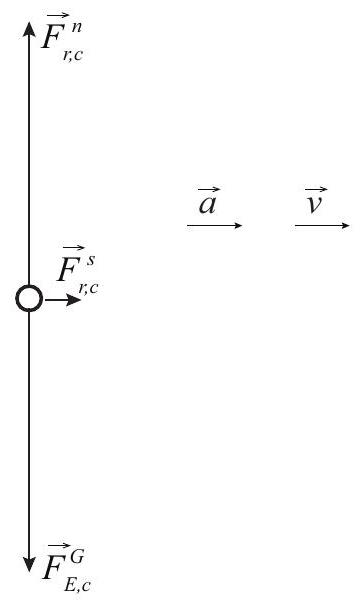
\includegraphics[max width=\textwidth, center]{2024_09_14_9969b06773f10b6936e8g-149}\\
(d) This is the opposite of part (a): the driver now relies on the force of static friction to slow down the car. The shortest stopping distance will correspond to the largest (in magnitude) acceleration, as per our old friend, Eq. (2.10):


\begin{equation*}
v_{f}^{2}-v_{i}^{2}=2 a \Delta x \tag{6.38}
\end{equation*}


In turn, the largest acceleration will correspond to the largest force. As explained in the chapter, the static friction force cannot exceed $\mu_{s} F^{n}$ (Eq. (6.29)). So, we have

$$
F_{\max }^{s}=\mu_{s} F^{n}=\mu_{s} m g
$$

since, in this case, we expect the normal force to be equal to the force of gravity. Then

$$
\left|a_{\max }\right|=\frac{F_{\max }^{s}}{m}=\frac{\mu_{s} m g}{m}=\mu_{s} g
$$

We can substitute this into Eq. (6.38) with a negative sign, since the acceleration acts in the opposite direction to the motion (and we are implicitly taking the direction of motion to be positive). Also note that the final velocity we want is zero, $v_{f}=0$. We get

$$
-v_{i}^{2}=2 a \Delta x=-2 \mu_{s} g \Delta x
$$

From here, we can solve for $\Delta x$ :

$$
\Delta x=\frac{v_{i}^{2}}{2 \mu_{s} g}=\frac{(13.4 \mathrm{~m} / \mathrm{s})^{2}}{2 \times 0.7 \times 9.81 \mathrm{~m} / \mathrm{s}^{2}}=13.1 \mathrm{~m}
$$

(e) Here is the free-body diagram. The interesting feature is that the force of static friction has reversed direction relative to parts (a)-(c). It is also much larger than before. (The forces are again to scale.)

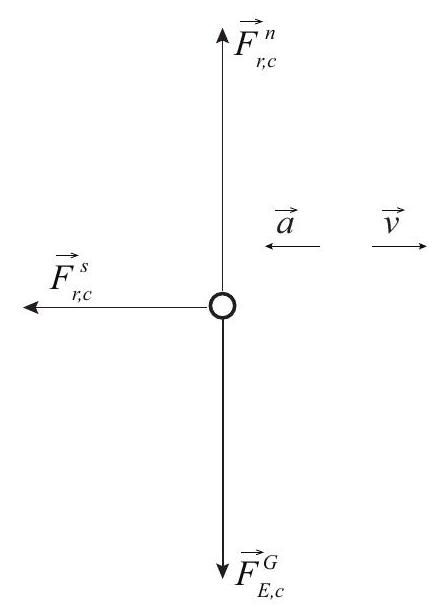
\includegraphics[max width=\textwidth, center]{2024_09_14_9969b06773f10b6936e8g-150}\\
(f) The math for this part is basically identical to that in part (d). The difference, physically, is that now you are dealing with the force of kinetic (or "sliding") friction, and that is always given by $F^{k}=\mu_{k} F^{n}$ (this is not an upper limit, it's just what $F^{k}$ is). So we have $a=-F^{k} / m=-\mu_{k} g$, and, just as before (but with $\mu_{k}$ replacing $\mu_{s}$ ),

$$
\Delta x=\frac{v_{i}^{2}}{2 \mu_{k} g}=\frac{(13.4 \mathrm{~m} / \mathrm{s})^{2}}{2 \times 0.2 \times 9.81 \mathrm{~m} / \mathrm{s}^{2}}=45.8 \mathrm{~m}
$$

This is a huge distance, close to half a football field! If these numbers are accurate, you can see that locking your brakes in the rain can have some pretty bad consequences.

\subsection*{6.7 Problems}
\section*{Problem 1}
(a) Draw a free-body diagram for the skydiver in Problem 4 of Chapter 5.\\
(b) What is the magnitude of the air drag force on the skydiver, after he reaches terminal speed?

\section*{Problem 2}
A book is sent sliding along a table with an initial velocity of $2 \mathrm{~m} / \mathrm{s}$. It slides for 1.5 m before coming to a stop. What is the coefficient of kinetic friction between the book and the table?

\section*{Problem 3}
You are pulling on a block of mass 4 kg that is attached, via a rope of negligible mass, to another block, of mass 6 kg . The coefficient of kinetic friction between the blocks and the surface on which they are sliding is $\mu_{k}$. You find that when you apply a force of 20 N , the whole thing moves at constant velocity.\\
(a) Draw a free-body diagram for each of the two blocks\\
(b) What is the coefficient of kinetic friction between the blocks and the surface?\\
(c) What is the tension in the rope?

\section*{Problem 4}
A box of mass 2 kg is sitting on top of a sled of mass 5 kg , which is resting on top of a frictionless surface (ice).\\
(a) What is the normal force exerted by the box on the sled? (And by the sled back on the box.)\\
(b) If you pull on the sled with a force of 35 N , how large does the coefficient of static friction, $\mu_{s}$, between the box and the sled have to be, in order for the box to move with the sled? Draw free-body diagrams for the box and for the sled under this assumption (that they move together).\\
(c) Suppose that $\mu_{s}$ is less than the value you got in part (b), so the box starts to slide back (relative to the sled). If the coefficient of kinetic friction $\mu_{k}$ between the box and the sled is 0.15 , what is the acceleration of the sled, and what is the acceleration of the box, while they are sliding relative to each other (so, before the box falls off, and while you are still pulling with a $35-\mathrm{N}$ force)? Draw again the free-body diagrams appropriate to this situation.

\section*{Problem 5}
You stick two objects together, one with a mass of 10 kg and one with a mass of 5 kg , using a glue that is supposed to be able to provide up to 19 N of force before it fails. Suppose you then pull on the 10 kg block with a force of 30 N .\\
(a) What is the acceleration of the whole system?\\
(b) What is the force exerted on the 5 kg block, and where does it come from? Does the glue hold?\\
(c) Now suppose you pull on the 5 kg block instead with the same force. Does the glue hold this time?

\section*{Problem 6}
Draw a free-body diagram for a $70-\mathrm{kg}$ person standing in an elevator carrying a $15-\mathrm{kg}$ backpack (do not consider the backpack a part of the person!). (a) if the elevator is not moving, and (b) if the elevator is accelerating downwards at $2 \mathrm{~m} / \mathrm{s}^{2}$. In each case, what is the magnitude of the normal force exerted on the person by the floor?

\section*{Chapter 7}
\section*{Impulse, Work and Power}
\subsection*{7.1 Introduction: work and impulse}
In physics, "work" (or "doing work") is what we call the process through which a force changes the energy of an object it acts on (or the energy of a system to which the object belongs). It is, therefore, a very technical term with a very specific meaning that may seem counterintuitive at times.

For instance, as it turns out, in order to change the energy of an object on which it acts, the force needs to be at least partly in line with the displacement of the object during the time it is acting. A force that is perpendicular to the displacement does no work-it does not change the object's energy.

Imagine a satellite in a circular orbit around the earth. The earth is constantly pulling on it with a force (gravity) directed towards the center of the orbit at any given time. This force is always perpendicular to the displacement, which is along the orbit, and so it does no work: the satellite moves always at the same speed, so its kinetic energy does not change.

The force does change the satellite's momentum, however: it keeps bending the trajectory, and therefore changing the direction (albeit not the magnitude) of the satellite's momentum vector. Of course, it is obvious that a force must change an object's momentum, because that is pretty much how we defined force anyway. Recall Eq. (6.1) for the average force on an object: $\vec{F}_{a v}=\Delta \vec{p} / \Delta t$. We can rearrange this to read


\begin{equation*}
\Delta \vec{p}=\vec{F}_{a v} \Delta t \tag{7.1}
\end{equation*}


For a constant force, the product of the force and the time over which it is acting is called the\\
impulse, usually denoted as $\vec{J}$


\begin{equation*}
\vec{J}=\vec{F} \Delta t \tag{7.2}
\end{equation*}


Clearly, the impulse given by a force to an object is equal to the change in the object's momentum (by Eq. (7.1)), as long as it is the only force (or, alternatively, the net force) acting on it. If the force is not constant, we break up the time interval $\Delta t$ into smaller subintervals and add all the pieces, pretty much as we did with Figure 1.5 in Chapter 1 in order to calculate the displacement for a variable velocity. Formally this results in an integral:


\begin{equation*}
\vec{J}=\int_{t_{i}}^{t_{f}} \vec{F}(t) d t \tag{7.3}
\end{equation*}


Graphically, the $x$ component of the impulse is equal to the area under the curve of $F_{x}$ versus time, and similarly for the other components. You will get to see how it works in a lab experiment this semester.

There is not a whole lot more to be said about impulse. The main lesson to be learned from Eq. (7.1) is that one can get a desired change in momentum - bring an object to a stop, for instance - either by using a large force over a short time, or a smaller force over a longer time. It is easy to see how different circumstances may call for different strategies: sometimes you may want to make the force as small as possible, if the object on which you are acting is particularly fragile; other times you may just need to make the time as short as possible instead.

Of course, to bring something to a stop you not only need to remove its momentum, but also its (kinetic) energy. If the former task takes time, the latter, it turns out, takes distance. Work is a much richer subject than impulse, not only because, as I have indicated above, the actual work done depends on the relative orientation of the force and displacement vectors, but also because there is only one kind of momentum, but many different kinds of energy, and one of the things that typically happens when work is done is the conversion of one type of energy into another.

So there is a lot of ground to cover, but we'll start small, in the next section, with the simplest kind of system, and the simplest kind of energy.

\subsection*{7.2 Work on a single particle}
Consider a particle that undergoes a displacement $\Delta x$ while a constant force $F$ acts on it. In one dimension, the work done by the force on the particle is defined by


\begin{equation*}
W=F \Delta x \quad(\text { constant force }) \tag{7.4}
\end{equation*}


and it is positive if the force and the displacement have the same sign (that is, if they point in the same direction), and negative otherwise.

In three dimensions, the force will be a vector $\vec{F}$ with components $\left(F_{x}, F_{y}, F_{z}\right)$, and the displacement, likewise, will be a vector $\Delta \vec{r}$ with components $(\Delta x, \Delta y, \Delta z)$. The work will be defined then as


\begin{equation*}
W=F_{x} \Delta x+F_{y} \Delta y+F_{z} \Delta z \tag{7.5}
\end{equation*}


This expression is an instance of what is known as the dot product (or inner product, or scalar product) of two vectors. Given two vectors $\vec{A}$ and $\vec{B}$, their dot product is defined, in terms of their components, as


\begin{equation*}
\vec{A} \cdot \vec{B}=A_{x} B_{x}+A_{y} B_{y}+A_{z} B_{z} \tag{7.6}
\end{equation*}


This can also be expressed in terms of the vectors' magnitudes, $|\vec{A}|$ and $|\vec{B}|$, and the angle they make, in the following form:


\begin{equation*}
\vec{A} \cdot \vec{B}=|\vec{A}||\vec{B}| \cos \phi \tag{7.7}
\end{equation*}


\begin{center}
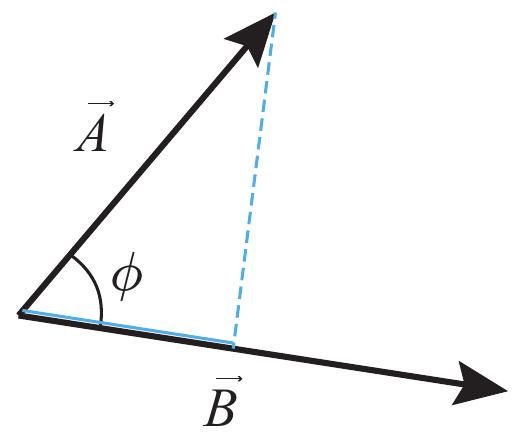
\includegraphics[max width=\textwidth]{2024_09_14_9969b06773f10b6936e8g-157}
\end{center}

Figure 7.1: Illustrating the angle $\phi$ to be used when calculating the dot product of two vectors by the formula (7.7). One way to think of this formula is that you take the projection of vector $\vec{A}$ onto vector $\vec{B}$ (indicated here by the blue lines), which is equal to $|\vec{A}| \cos \phi$, then multiply that by the length of $\vec{B}$ (or vice-versa, of course).

Figure 7.1 shows what I mean by the angle $\phi$ in this expression. The equality of the two definitions, Eqs. (7.6) and (7.7), is proved in mathematics textbooks. The advantage of Eq. (7.7) is that it is independent of the choice of a system of coordinates.

Using the dot product notation, the work done by a constant force can be written as


\begin{equation*}
W=\vec{F} \cdot \Delta \vec{r} \tag{7.8}
\end{equation*}


Equation (7.7) then shows that, as I mentioned in the introduction, when the force is perpendicular to the displacement $\left(\phi=90^{\circ}\right)$ the work it does is zero. You can also see this directly from Eq. (7.5), by choosing the $x$ axis to point in the direction of the force (so $F_{y}=F_{z}=0$ ), and the displacement to point along any of the other two axes (so $\Delta x=0$ ): the result is $W=0$.

If the force is not constant, again we follow the standard procedure of breaking up the total displacement into pieces that are short enough that the force may be taken to be constant over\\
each of them, calculating all those (possibly very small) "pieces of work," and adding them all together. In one dimension, the final result can be expressed as the integral


\begin{equation*}
W=\int_{x_{i}}^{x_{f}} F(x) d x \quad \text { (variable force) } \tag{7.9}
\end{equation*}


So the work is given by the "area" under the $F$-vs- $x$ curve. In more dimensions, we have to write a kind of multivariable integral known as a line integral. That is advanced calculus, so we will not go there this semester.

\subsection*{7.2.1 Work done by the net force, and the Work-Energy Theorem}
So much for the math and the definitions. Where does the energy come in? Let us suppose that $F$ is either the only force or the net force on the particle - the sum of all the forces acting on the particle. Again, for simplicity we will assume that it is constant (does not change) while the particle undergoes the displacement $\Delta x$. However, now $\Delta x$ and $F_{n e t}$ are related: a constant net force means a constant acceleration, $a=F_{\text {net }} / m$, and for constant acceleration we know the formula $v_{f}^{2}-v_{i}^{2}=2 a \Delta x$ applies. Therefore, we can write


\begin{equation*}
W_{n e t}=F_{n e t} \Delta x=m a \Delta x=m \frac{1}{2}\left(v_{f}^{2}-v_{i}^{2}\right) \tag{7.10}
\end{equation*}


which is to say


\begin{equation*}
W_{n e t}=\Delta K \tag{7.11}
\end{equation*}


In words, the work done by the net force acting on a particle as it moves equals the change in the particle's kinetic energy in the course of its displacement. This result is often referred to as the Work-Energy Theorem.

As you may have guessed from our calling it a "theorem," the result (7.11) is very general. It holds in three dimensions, and it holds also when the force isn't constant throughout the displacementyou just have to use the correct equation to calculate the work in those cases. It would apply to the work done by the net force on an extended object, also, provided it is OK to treat the extended object as a particle - so basically, a rigid object that is moving as a whole and not doing anything fancy such as spinning while doing so.

Another possible direction in which to generalize (7.11) might be as follows. By definition, a "particle" has no other kind of energy, besides (translational) kinetic energy. Also, and for the same reason (namely, the absence of internal structure), it has no "internal" forces - all the forces acting on it are external. So-for this very simple system - we could rephrase the result (7.11) by saying that the work done by the net external force acting on the system (the particle in this case) is equal to the change in its total energy. It is in fact in this form that we will ultimately generalize (7.11) to deal with arbitrary systems.

Before we go there, however, I would like to take a little detour to explore another "reasonable" extension of the result (7.11), as well as its limitations.

\subsection*{7.3 The "center of mass work"}
All the physics I used in order to derive the result (7.11) was $F=m a$, and the expression $v_{f}^{2}-v_{i}^{2}=$ $2 a \Delta x$, which applies whenever we have motion with constant acceleration. Now, we know that for an arbitrary system, of total mass $M, F_{\text {ext,net }}=M a_{c m}$ [see Eq. (6.11)]. That is enough, then, to ensure that, if $F_{\text {ext,net }}$ is a constant, we will have


\begin{equation*}
F_{e x t, n e t} \Delta x_{c m}=\Delta K_{c m} \tag{7.12}
\end{equation*}


where $K_{c m}$, the translational kinetic energy, is, as usual, $K_{c m}=\frac{1}{2} M v_{c m}^{2}$, and $\Delta x_{c m}$ is the displacement of the center of mass. The result (7.12) holds for an arbitrary system, as long as $F_{\text {ext,net }}$ is constant, and can be generalized by means of an integral (as in Eq. (7.9)) when it is variable.

So it seems that we could define the left-hand side of Eq. (7.12) as "the work done on the center of mass," and take that as the natural generalization to a system of the result (7.11) for a particle. Most physicists would, in fact, be OK with that, but educators nowadays frown on that idea, for a couple of reasons.

First, it seems that it is essential to the notion of work that one should multiply the force by the displacement of the object on which it is acting. More precisely, in the definition (7.4), we want the displacement of the point of application of the force ${ }^{1}$. But there are many examples of systems where there is nothing at the precise location of the center of mass, and certainly no force acting precisely there.

This is not necessarily a problem in the case of a rigid object which is not doing anything funny, just moving as a whole so that every part has the same displacement, because then the displacement of the center of mass would simply stand for the displacement of any point at which an external force might actually be applied. But for many deformable systems, this would not be case. In fact, for such systems one can usually show that $F_{\text {ext,net }} \Delta x_{c m}$ is actually not the work done on the system by the net external force. A simple example of such a system is shown below, in Figure 7.2.

\footnotetext{${ }^{1}$ As the name implies, this is the precise point at which the force is applied. For contact forces (other than friction; see later), this is easily identified. For gravity, a sum over all the forces exerted on all the particles that make up the object may be shown to be equivalent to a single resultant force acting at a point called the center of gravity, which, for our purposes (objects in uniform or near-uniform gravitational fields) will be the same as the center of mass.
}\begin{center}
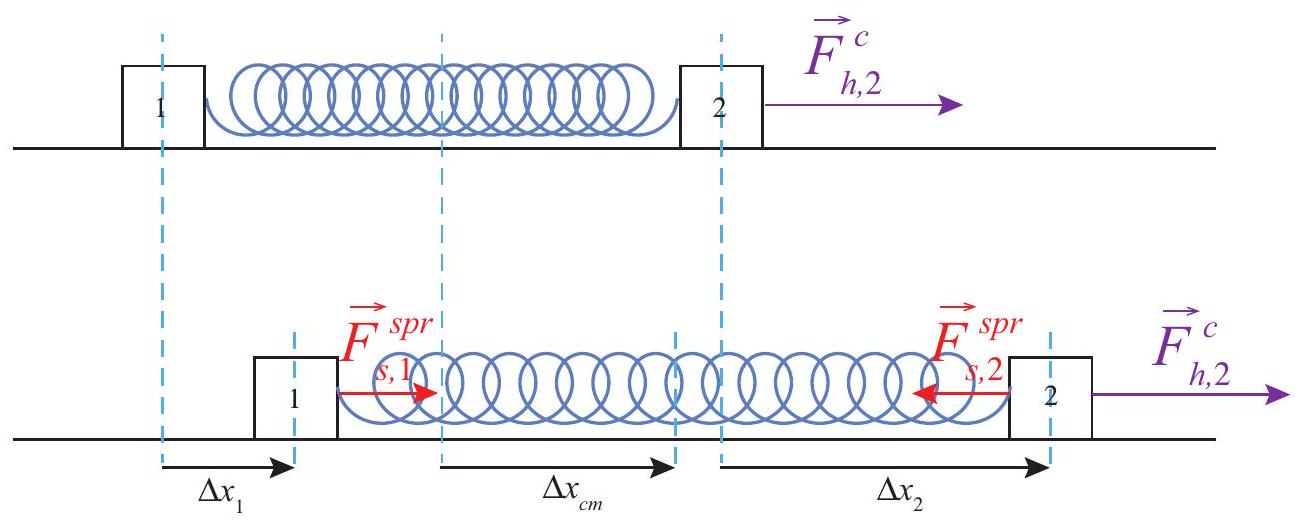
\includegraphics[max width=\textwidth]{2024_09_14_9969b06773f10b6936e8g-160}
\end{center}

Figure 7.2: A system of two blocks connected by a spring. A constant external force, $\vec{F}_{h, 2}^{c}$, is applied to the block on the right. Initially the spring is relaxed, but as soon as block 2 starts to move it stretches, pulling back on block 2 and pulling forward on block 1. Because of the stretching of the spring, the displacements $\Delta x_{1}, \Delta x_{c m}$ and $\Delta x_{2}$ are all different, and the work done by the external force, $F_{h, 2}^{c} \Delta x_{2}$, is different from the "center of mass work" $F_{h, 2}^{c} \Delta x_{c m}$.

In this figure, the two blocks are connected by a spring, and the external force is applied to the block on the right (block 2). If the blocks have the same mass, the center of mass of the system is a point exactly halfway between them. If the spring starts in its relaxed state, it will stretch at first, so that the center of mass will lag behind block 2, and $F_{h, 2}^{c} \Delta x_{2}$, which is the quantity that we should properly call the "work done by the net external force" will not be equal to $F_{h, 2}^{c} \Delta x_{c m}$.

We find ourselves, therefore, with a very general and potentially rather useful result, Eq. (7.12), that looks a lot like it should be "the work done on the system by the net external force" but, in fact, is that only sometimes. On the other hand, the result is so useful that simply referring to it all the time by "Eq. (7.12)" will not do. I propose, therefore, to call it the "center of mass work," in between quotation marks, just so we all know what we are talking about, and remember the caveats that go with it.

We can now move to the real theorem relating the work of the external forces on a system to the change in its energy. What we have seen so far are really just straightforward applications of Newton's second law. The main result coming up is deeper than that, since it involves also, ultimately, the principle of conservation of energy.

\subsection*{7.4 Work done on a system by all the external forces}
Consider the most general possible system, one that might contain any number of particles, with possibly many forces, both internal and external, acting on each of them. I will again, for simplicity,\\
start by considering what happens over a time interval so short that all the forces are approximately constant (the final result will hold for arbitrarily long time intervals, just by adding, or integrating, over many such short intervals). I will also work explicitly only the one-dimensional case, although again that turns out to not be a real restriction.

Let then $W_{\text {all, } 1}$ be the work done on particle 1 by all the forces acting on it, $W_{\text {all, }}$ the work done on particle 2, and so on. The total work is the sum $W_{\text {all,sys }}=W_{\text {all }, 1}+W_{\text {all }, 2}+\ldots$ However, by the results of section 7.2 , we have $W_{\text {all, } 1}=\Delta K_{1}$ (the change in kinetic energy of particle 1 ), $W_{\text {all }, 2}=\Delta K_{2}$, and so on, so adding all these up we get


\begin{equation*}
W_{\text {all,sys }}=\Delta K_{\text {sys }} \tag{7.13}
\end{equation*}


where $\Delta K_{\text {sys }}$ is the change in kinetic energy of the whole system.

So far, of course, this is nothing new. To learn something else we need to look next at the work done by the internal forces. It is helpful here to start by considering the "no-dissipation case" in which all the internal forces can be derived from a potential energy ${ }^{2}$. We will consider the case where dissipative processes happen inside the system after we have gained a full understanding of the result we will obtain for this simpler case.

\subsection*{7.4.1 The no-dissipation case}
The internal forces are, by definition, forces that arise from the interactions between pairs of particles that are both inside the system. Because of Newton's 3 rd law, the force $F_{12}$ (we will omit the "type" superscript for now) exerted by particle 1 on particle 2 must be the negative of $F_{21}$, the force exerted by particle 2 on particle 1. Hence, the work associated with this interaction for this pair of particles can be written


\begin{equation*}
W(1,2)=F_{12} \Delta x_{2}+F_{21} \Delta x_{1}=F_{12}\left(\Delta x_{2}-\Delta x_{1}\right) \tag{7.14}
\end{equation*}


Notice that $\Delta x_{2}-\Delta x_{1}$ can be rewritten as $x_{2, f}-x_{2, i}-x_{1, f}+x_{1, i}=x_{12, f}-x_{12, i}=\Delta x_{12}$, where $x_{12}=x_{2}-x_{1}$ is the relative position coordinate of the two particles. Therefore,


\begin{equation*}
W(1,2)=F_{12} \Delta x_{12} \tag{7.15}
\end{equation*}


Now, if the interaction in question is associated with a potential energy, as I showed in section 6.2, $F_{12}=-d U / d x_{12}$. Assume the displacement $\Delta x_{12}$ is so small that we can replace the derivative by just the ratio $\Delta U / \Delta x_{12}$ (which is consistent with our assumption that the force is approximately constant over the time interval considered); the result will then be


\begin{equation*}
W(1,2)=F_{12} \Delta x_{12} \simeq-\frac{\Delta U}{\Delta x_{12}} \Delta x_{12}=-\Delta U \tag{7.16}
\end{equation*}


\footnotetext{${ }^{2}$ Or else they do no work at all: the magnetic force between moving charges is an example of the latter.
}Adding up very many such "infinitesimal" displacements will lead to the same final result, where $\Delta U$ will be the change in the potential energy over the whole process. This can also be proved using calculus, without any approximations:


\begin{equation*}
W(1,2)=\int_{x_{12, i}}^{x_{12, f}} F_{12} d x_{12}=-\int_{x_{12, i}}^{x_{12, f}} \frac{d U}{d x_{12}} d x_{12}=-\Delta U \tag{7.17}
\end{equation*}


We can apply this to every pair of particles and every internal interaction, and then add up all the results. On one side, we will get the total work done on the system by all the internal forces; on the other side, we will get the negative of the change in the system's total internal energy:


\begin{equation*}
W_{\text {int,sys }}=-\Delta U_{\text {sys }} \tag{7.18}
\end{equation*}


In words, the work done by all the (conservative) internal forces is equal to the change in the system's potential energy.

Let us now put Eqs. (7.13) and (7.18) together: the difference between the work done by all the forces and the work done by the internal forces is, of course, the work done by the external forces, but according to Eqs. (7.13) and (7.18), this is equal to


\begin{equation*}
W_{\text {ext }, \text { sys }}=W_{\text {all,sys }}-W_{\text {int }, \text { sys }}=\Delta K_{\text {sys }}+\Delta U_{\text {sys }} \tag{7.19}
\end{equation*}


which is the change in the total mechanical (kinetic plus potential) energy of the system. If we further assume that the system, in the absence of the external forces, is closed, then there are no other processes (such as the absorption of heat) by which the total energy of the system might change, and we get the simple result that the work done by the external forces equals the change in the system's total energy:


\begin{equation*}
W_{\text {ext,sys }}=\Delta E_{\text {sys }} \tag{7.20}
\end{equation*}


As a first application of the result (7.20), consider again the blocks connected by a spring shown in Fig. 2. You can see now why the work done by the external force $F_{h, 2}^{c}$ has to be different, and in fact larger, than the "center of mass work": the latter only gives us the change in the translational energy, but the former has to give us the change in the total energy-translational, convertible, and potential:


\begin{align*}
F_{h, 2}^{c} \Delta x_{c m} & =\Delta K_{c m} \\
F_{h, 2}^{c} \Delta x_{2} & =\Delta K_{c m}+\Delta K_{c o n v}+\Delta U^{s p r} \tag{7.21}
\end{align*}


As another example, imagine you throw a ball of mass $m$ upwards (see Figure 7.3, next page), and it reaches a maximum height $h$ above the point where your hand started to move. Let us define the system to be the ball and the earth, so the force exerted by your hand is an external force. Then you do work on the system during the throw, which in the figure is the interval, from A to B, during which your hand is on contact with the ball. The bar diagram on the side shows that some of this work goes into increasing the system's (gravitational) potential energy (because the\\
ball goes up a little while in contact with your hand), and the rest, which is typically most of it, goes into increasing the system's kinetic energy (in this case, just the ball's; the earth's kinetic energy does not change in any measurable way!).\\
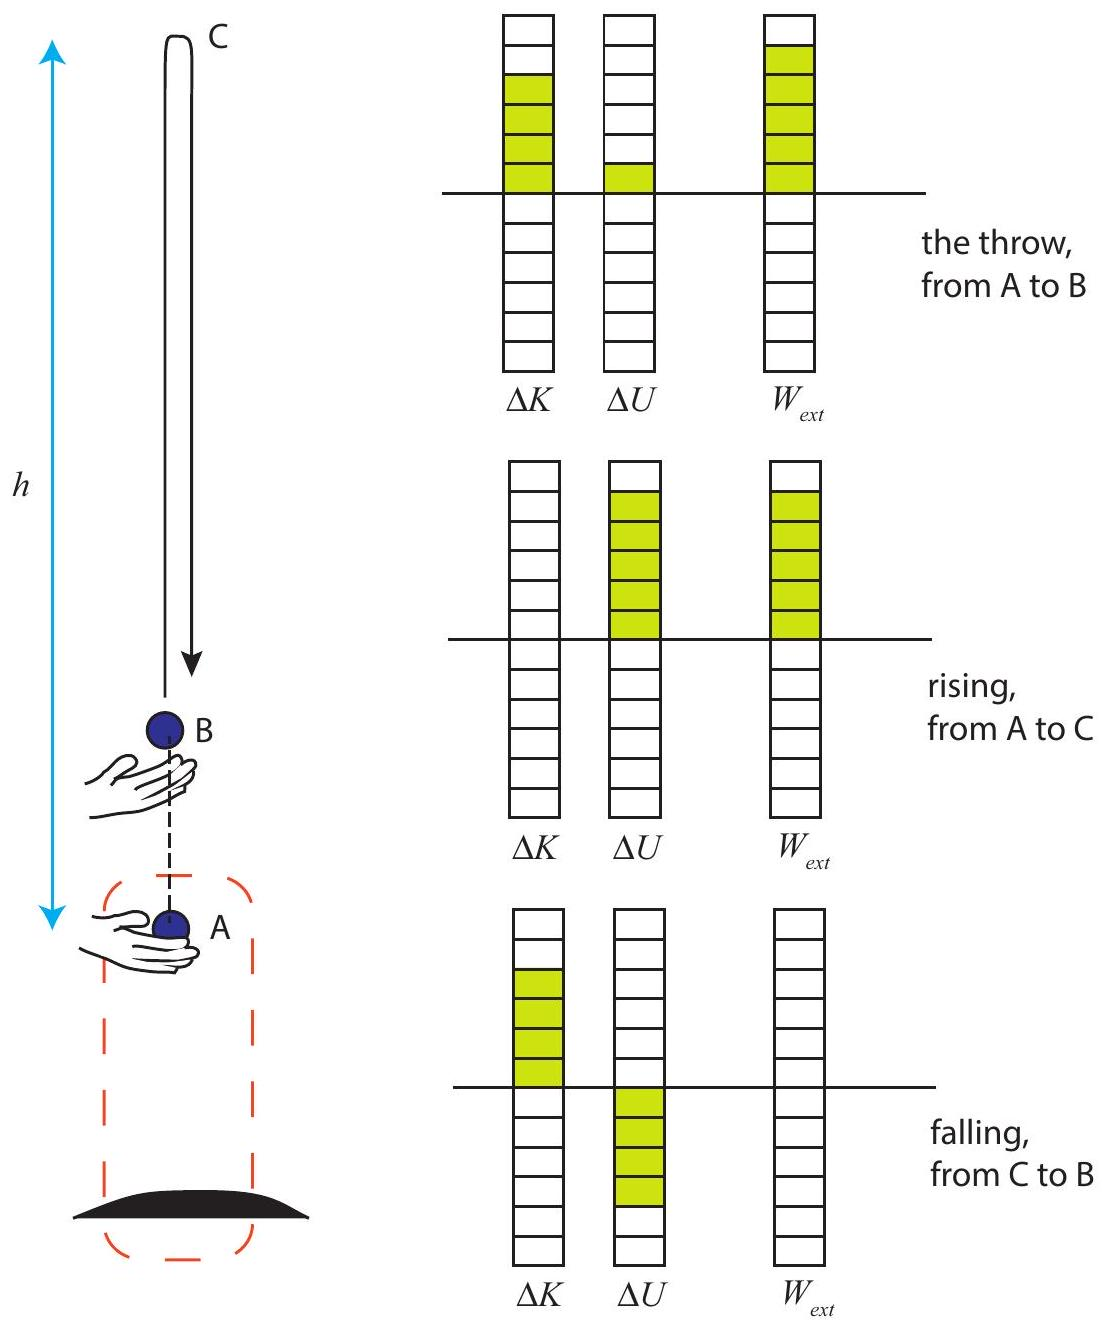
\includegraphics[max width=\textwidth, center]{2024_09_14_9969b06773f10b6936e8g-163}

Figure 7.3: Tossing a ball into the air. We consider the system formed by the ball and the earth. The force exerted by the hand (which is in contact with the ball from point A to point B ) is therefore an external force. The diagrams show the system's energy balance over three different intervals.

So how much work did you actually do? If we knew the distance from A to B, and the magnitude of the force you exerted, and if we could assume that your force was constant throughout, we could calculate $W$ from the definition (7.4). But in this case, and many others like it, it is actually easier to find out how much total energy the system gained and just use Eq. (7.20). To find $\Delta E$ in\\
practice, all we have to do is see how high the ball rises. At the ball's maximum height (point C), as the second diagram shows, all the energy in the system is gravitational potential energy, and (as long as the system stays closed), all that energy is still equal to the work you did initially, so if the distance from A to C is $h$ you must have done an amount of work


\begin{equation*}
W_{\text {you }}=\Delta U^{G}=m g h \tag{7.22}
\end{equation*}


The third diagram in Figure 7.3 shows the work-energy balance for another time interval, during which the ball falls from C to B. Over this time, no external forces act on the ball (recall we have taken the system to be the ball and the earth, so gravity is an internal force). Then, the work done by the external forces is zero, and the change in the total energy of the system is also zero. The diagram just shows an increase in kinetic energy at the expense of an equal decrease in potential energy.

What about the work done by the internal forces? Eq. (7.18) tells us that this work is equal to the negative of the change in potential energy. In this case, the internal force is gravity, and the corresponding energy is gravitational potential energy. This change in potential energy is clearly visible in all the diagrams; however, when you add to it the change in kinetic energy, the result is always equal to the work done by the external force only. Put otherwise, the internal forces do not change the system's total energy, they just "redistribute" it among different kinds - as in, for instance, the last diagram in Fig. 7.3, where you can clearly see that gravity is causing the kinetic energy of the system to increase at the expense of the potential energy.

We will use diagrams like the ones in Figure 7.3 to look at the work-energy balance for different systems. The idea is that the sum of all the columns on the left (the change in the system's total energy) has to equal the result on the far-right column (the work done by the net external force): that is the content of the theorem (7.20). Note that, unlike the energy diagrams we used in Chapter 5 , these columns represent changes in the energy, so they could be positive or negative.

Just as for the earlier energy diagrams, the picture we get will be different, even for the same physical situation, depending on the choice of system. This is illustrated in Figure 7.4 below (next page), where I have taken the same throw shown in Fig. 7.3, but now the system I'm looking at is the ball only. This means gravity is now an external force, as is the force of the hand, and the ball only has kinetic energy. Normally one would show the sum of the work done by the two external forces on a single column, but here I have chosen to break it up into two columns for clarity.

As you can see, during the throw the hand does positive work, whereas gravity does a comparatively small amount of negative work, and the change in kinetic energy is the sum of the two. For the longer interval from A to C (second diagram), gravity continues to do negative work until all the kinetic energy of the ball is gone. For the interval from C to B , the only external force is gravity, which now does positive work, equal to the increase in the ball's kinetic energy.

\begin{center}
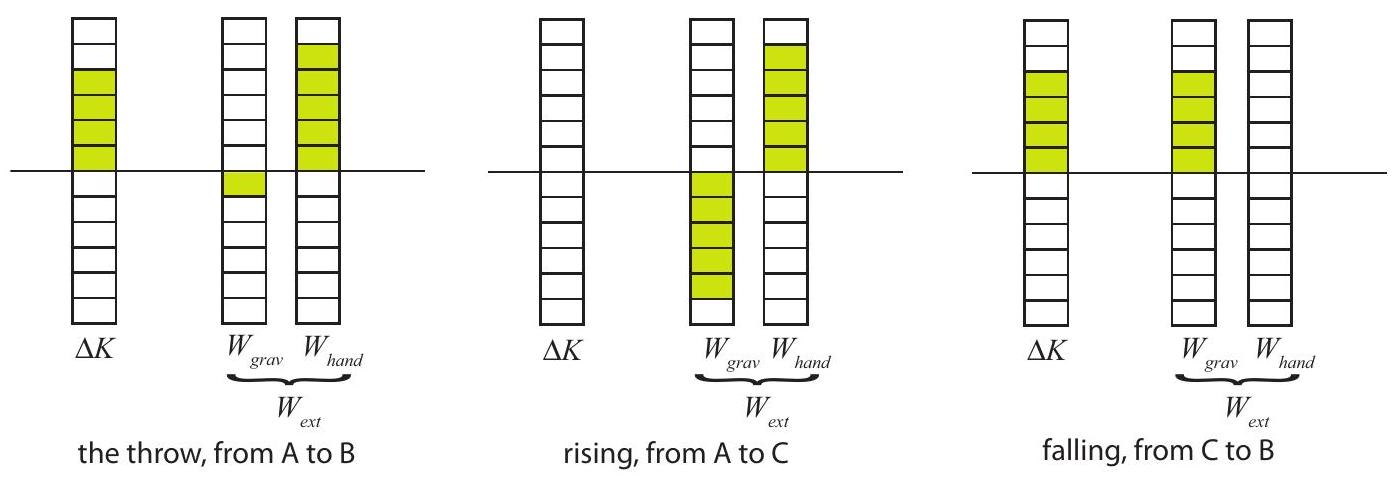
\includegraphics[max width=\textwidth]{2024_09_14_9969b06773f10b6936e8g-165}
\end{center}

Figure 7.4: Work-energy balance diagrams for the same toss illustrated in Fig. 7.3, but now the system is taken to be the ball only.

Of course, the numerical value of the actual work done by any particular force does not depend on our choice of system: in each case, gravity does the same amount of work in the processes illustrated in Fig. 7.4 as in those illustrated in Fig. 7.3. The difference, however, is that for the system in Fig. 7.4, gravity is an external force, and now the work it does actually changes the system's total energy, because the gravitational potential energy is now not included in that total.

Formally, it works like this: in the case shown in Fig. 7.3, where the system is the ball and the earth, we have $\Delta K+\Delta U^{G}=W_{\text {hand }}$. By the result (7.18), however, we have $\Delta U^{G}=-W_{\text {grav }}$, and so this equation can be rearranged to read $\Delta K=W_{\text {grav }}+W_{\text {hand }}$, which is just the result (7.20) when the system is the ball alone.

Ultimately, the reason we emphasize the importance of the choice of system is to prevent double counting: if you want to count the work done by gravity as contributing to the change in the system's total energy, it means that you are, implicitly, treating gravity as an external force, and therefore your system must be something that does not have, by itself, gravitational potential energy (the case of the ball in Figure 7.4); conversely, if you insist on counting gravitational potential energy as contributing to the system's total energy, then you must treat gravity as an internal force, and leave it out of the calculation of the work done on the system by the external forces, which are the only ones that can change the system's total energy.

\subsection*{7.4.2 The general case: systems with dissipation}
We are now ready to consider what happens when some of the internal interactions in a system are not conservative. There are two key observations to keep in mind: first, of course, that energy will always be conserved in a closed system, regardless of whether the internal forces are "conservative" or not: if they are not, it merely means that they will convert some of the "organized," mechanical energy, into disorganized (primarily thermal) energy.

The second observation is that the work done by an external force on a system does not depend on where the force comes from - that is to say, what physical arrangement we use to produce the force. Only the value of the force at each step and the displacement of the point of application are involved in the definition (7.9). This means, in particular, that we can use a conservative interaction to do the work for us. It turns out, then, that the generalization of the result (7.20) to apply to all sorts of interactions becomes straightforward.

To see the idea, consider, for example, the situation in Figure 7.5 below. This is essentially the same as Figure 6.2, which we analyzed in detail from the perspective of forces and accelerations in the previous chapter. Here I have broken it up into two systems. System A, outlined in blue, consists of block 1 and the surface on which it slides, and includes a dissipative interaction-namely, kinetic friction-between the block and the surface. The force doing work on this system is the tension force from the rope, $\vec{F}_{r, 1}^{t}$.

\begin{center}
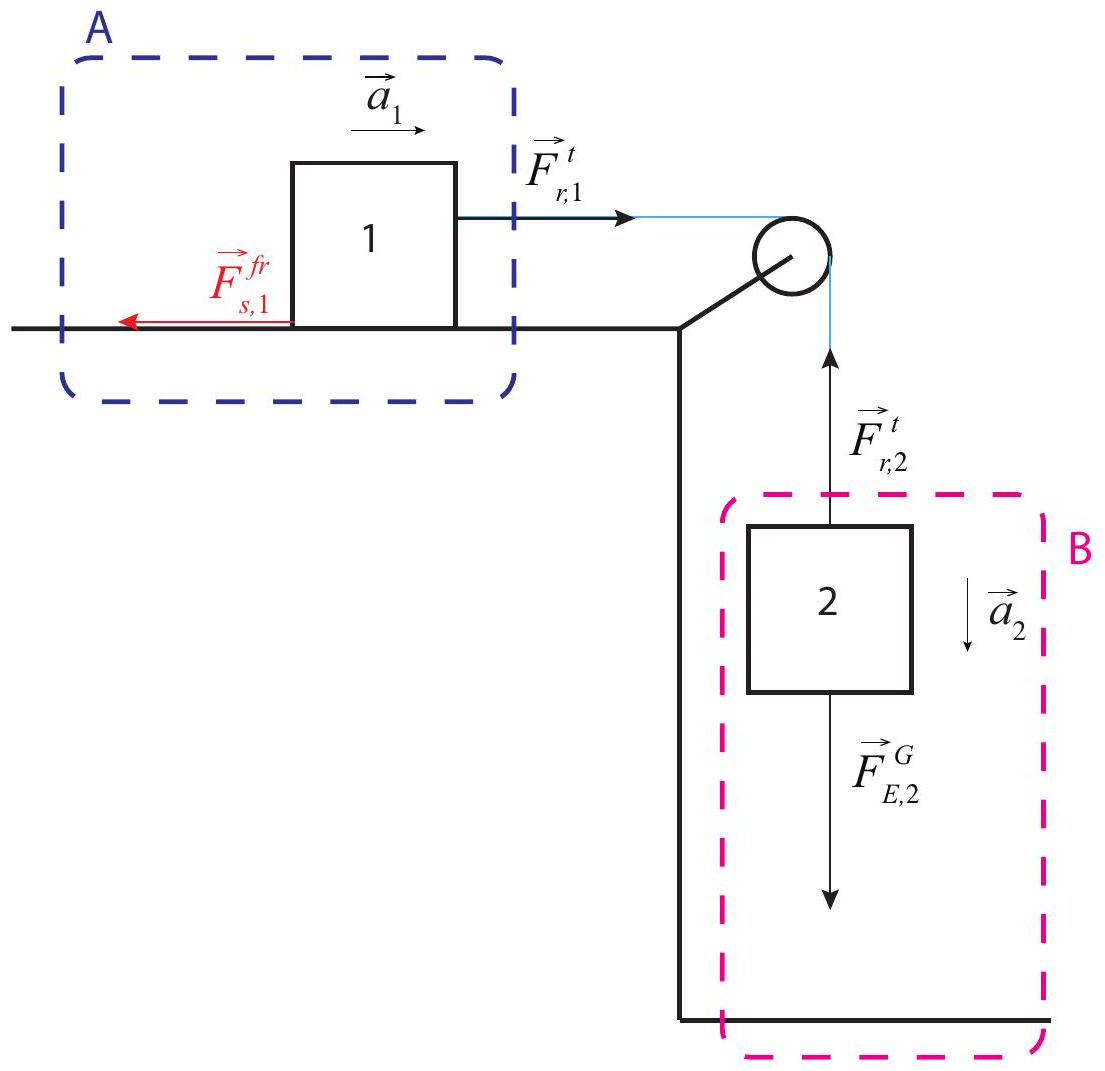
\includegraphics[max width=\textwidth]{2024_09_14_9969b06773f10b6936e8g-166}
\end{center}

Figure 7.5: Block sliding on a surface, with friction, being pulled by a rope attached to a block falling under the action of gravity. The motion of this system was solved for in Section 6.3.

Because the rope is assumed to have negligible mass, this force is the same in magnitude as the\\
force $\vec{F}_{r, 2}^{t}$ that is doing negative work on system B. System B, outlined in magenta, consists of block 2 and the earth and thus it includes only one internal interaction, namely gravity, which is conservative. This means that we can immediately apply the theorem (7.20) to it, and conclude that the work done on B by $\vec{F}_{r, 2}^{t}$ is equal to the change in system B's total energy:


\begin{equation*}
W_{r, B}=\Delta E_{B} \tag{7.23}
\end{equation*}


However, since the rope is inextensible, the two blocks move the same distance in the same time, and the force exerted on each by the rope is the same in magnitude, so the work done by the rope on system A is equal in magnitude but opposite in sign to the work it does on system B :


\begin{equation*}
W_{r, A}=-W_{r, B}=-\Delta E_{B} \tag{7.24}
\end{equation*}


Now consider the total system formed by A+B. Assuming it is a closed system, its total energy must be constant, and so any change in the total energy of B must be equal and opposite the corresponding change in the total energy of A: $\Delta E_{B}=-\Delta E_{A}$. Therefore,


\begin{equation*}
W_{r, A}=-\Delta E_{B}=\Delta E_{A} \tag{7.25}
\end{equation*}


So we conclude that the work done by the external force on system A must be equal to the total change in system A's energy. In other words, Eq. (7.20) applies to system A as well, as it does to system B, even though the interaction between the parts that make up system A is dissipative.

Although I have shown this to be true just for one specific example, the argument is quite general: if I use a conservative system B to do some work on another system A, two things happen: first, by virtue of (7.20), the work done by B comes at the expense of its total energy, so $W_{e x t, A}=-\Delta E_{B}$. Second, if A and B together form a closed system, the change in A's energy must be equal and opposite the change in B's energy, so $\Delta E_{A}=-\Delta E_{B}=W_{\text {ext, } A}$. So the result (7.20) holds for A, regardless of whether its internal interactions are conservative or not.

What is essential in the above reasoning is that A and B together should form a closed system, that is, one that does not exchange energy with its environment. It is very important, therefore, if we want to apply the theorem (7.20) to a general system - that is, one that includes dissipative interactions - that we draw the boundary of the system in such a way as to ensure that no dissipation is happening at the boundary. For example, in the situation illustrated in Fig. 7.5, if we want the result (7.25) to apply we must take system A to include both block 1 and the surface on which it slides. The reason for this is that the energy "dissipated" by kinetic friction when two objects rub together goes into both objects. So, as the block slides, kinetic friction is converting some of its kinetic energy into thermal energy, but not all this thermal energy stays inside block 1. Put otherwise, in the presence of friction, block 1 by itself is not a closed system: it is "leaking" energy to the surface. On the other hand, when you include (enough of) the surface in the system, you can be sure to have "caught" all the dissipated energy, and the result (7.20) applies.

\subsection*{7.4.3 Energy dissipated by kinetic friction}
In the situation illustrated in Fig. 7.5, we might calculate the energy dissipated by kinetic friction by indirect means. For instance, we can use the fact that the energy of system A is of two kinds, kinetic and "dissipated," and therefore, by theorem (7.20), we have


\begin{equation*}
\Delta K+\Delta E_{\text {diss }}=F_{r, 1}^{t} \Delta x_{1} \tag{7.26}
\end{equation*}


Back in section 6.3, we used Newton's laws to solve for the acceleration of this system and the tension in the rope; using those results, we can calculate the displacement $\Delta x_{1}$ over any time interval, and the corresponding change in $K$, and then we can solve Eq. (7.26) for $\Delta E_{\text {diss }}$.

If we do this, we will find out that, in fact, the following result holds,


\begin{equation*}
\Delta E_{d i s s}=-F_{s, 1}^{k} \Delta x_{1} \tag{7.27}
\end{equation*}


where $F_{s, 1}^{k}$ is the force of kinetic friction exerted by the surface on block 1, and must be understood to be negative in this equation (so that $\Delta E_{\text {diss }}$ will come out positive, as it must be).

It is tempting to think of the product $F_{s, 1}^{k} \Delta x$ as the work done by the force of kinetic friction on the block, and most of the time there is nothing wrong with that, but it is important to realize that the "point of application" of the friction force is not a single point: rather, the force is "distributed," that is to say, spread over the whole contact area between the block and the surface. As a consequence of this, a more general expression for the energy dissipated by kinetic friction between an object $o$ and a surface $s$ should be


\begin{equation*}
\Delta E_{\text {diss }}=\left|F_{s, o}^{k}\right|\left|\Delta x_{s o}\right| \tag{7.28}
\end{equation*}


where I am using the Chapter 1 subscript notation $x_{A B}$ to refer to "the position of $B$ in the frame of $A$ " (or "relative to $A$ "); in other words, $\Delta x_{s o}$ is the change in the position of the object relative to the surface or, more simply, the distance that the object and the surface slip past each other (while rubbing against each other, and hence dissipating energy). If the surfaces is at rest (relative to the Earth), $\Delta x_{s o}$ reduces to $\Delta x_{E o}$, the displacement of the object in the Earth reference frame, and we can remove the subscript $E$, as we typically do, for simplicity; however, in the rare cases when both the surface and the objet are moving (as in part (c) of Problem 3 in Chapter 6, the sled problem) what matters is how far they move relative to each other. In that case we have $\left|\Delta x_{s o}\right|=\left|\Delta x_{o}-\Delta x_{s}\right|$ (with both $\Delta x_{o}$ and $\Delta x_{s}$ measured in the Earth reference frame).

\subsection*{7.5 Power}
By "power" we mean the rate at which work is done, which is to say, the rate at which energy is taken in, or given out, or converted from one form to another. The SI unit of power is the watt (W),\\
which is equal to $1 \mathrm{~J} / \mathrm{s}$. The average power going into or coming out of a system by mechanical means, that is to say, through the action of a force applied at a point undergoing a displacement $\Delta x$, will be


\begin{equation*}
P_{a v}=\frac{\Delta E}{\Delta t}=\frac{W}{\Delta t}=F \frac{\Delta x}{\Delta t} \tag{7.29}
\end{equation*}


assuming the force is constant. Note that in the limit when $\Delta t$ goes to zero, this gives us the instantaneous power associated with the force $F$ as


\begin{equation*}
P=F v \tag{7.30}
\end{equation*}


where $v$ is the (instantaneous) velocity of the point of application of the force. This one-dimensional result generalizes to three dimensions as


\begin{equation*}
P=\vec{F} \cdot \vec{v} \tag{7.31}
\end{equation*}


using again the dot product notation.\\
An important goal of this chapter has been to develop a set of tools that you may use to find out where power is spent, and how much: in any practical situation, which systems are giving energy and which are taking it in, what forms of energy conversion are taking place, and where and through which means are the exchanges and conversions happening. These are extremely important practical questions; the problems and exercises that you will see here will give you a feel for the variety of situations that can already be analyzed by this "systems-based" approach, but in a way they will still do little more than scratch the surface.

\subsection*{7.6 In summary}
\begin{enumerate}
  \item The change in the momentum of a system produced by a force $\vec{F}$ acting over a time $\Delta t$ is given the name of "impulse" and denoted by $\vec{J}$. For a constant force, we have $\vec{J}=\Delta \vec{p}=\vec{F} \Delta t$.
  \item Work, or "doing work" is the name given in physics to the process by which an applied force brings about a change in the energy of an object, or of a system that contains the object on which the force is acting.
  \item The work done by a constant force $\vec{F}$ acting on an object or system is given by $W=\vec{F} \cdot \Delta \vec{r}$, where the dot represents the "dot" or "scalar" product of the two vectors, and $\Delta \vec{r}$ is the displacement undergone by the point of application of the force while the force is acting. If the force is perpendicular to the displacement, it does no work.
  \item For a system that is otherwise closed, the net sum of the amounts of work done by all the external forces is equal to the change in the system's total energy, when all the types of energy are included. Note that, for deformable systems, the displacement of the point of application may be different for different forces.
  \item The result in 4 above holds only provided the boundary of the system is not drawn at a physical surface on which dissipation occurs. Put otherwise, kinetic friction or other similar dissipative forces (drag, air resistance) must be included as internal, not external forces.
  \item The work done by the internal forces in a closed system results only in the conversion of one type of energy into another, always keeping the total energy constant.
  \item For a system with no internal energy, like a particle, the work done by all the external forces equals the change in kinetic energy. This result is sometimes called the Work-Energy theorem in a narrow sense.
  \item For any system, if $\vec{F}_{\text {ext,net }}$ (assumed constant) is the sum of all the external forces, the following result holds:
\end{enumerate}

$$
\vec{F}_{\text {ext,net }} \cdot \Delta \vec{r}_{c m}=\Delta K_{c m}
$$

where $K_{c m}$ is the translational (or "center of mass") kinetic energy, and $\Delta \vec{r}_{c m}$ is the displacement of the center of mass. This is only sometimes equal to the net work done on the system by the external forces.\\
9. For an object $o$ sliding on a surface $s$, the energy dissipated by kinetic friction can be directly calculated as

$$
\Delta E_{\text {diss }}=\left|F_{s, o}^{k}\right|\left|\Delta x_{s o}\right|
$$

where $\left|\Delta x_{s o}\right|=\left|\Delta x_{o}-\Delta x_{s}\right|$ is the distance that the two surfaces in contact slip past each other. This expression, with a negative sign, can be used to take the place of the "work done by friction" in applications of the results 7 and 8 above to systems involving kinetic friction forces.\\
10. The power of a system is the rate at which it does work, that is to say, takes in or gives up energy: $P_{a v}=\Delta E / \Delta t$. When this is done by means of an applied force $F$, the instantaneous power can be written as $P=F v$, or, in three dimensions, $\vec{F} \cdot \vec{v}$.

\subsection*{7.7 Examples}
\subsection*{7.7.1 Braking}
Suppose you are riding your bicycle and hit the brakes to come to a stop. Assuming no slippage between the tire and the road:\\
(a) Which force is responsible for removing your momentum? (By "you" I mean throughout "you and the bicycle.")\\
(b) Which force is responsible for removing your kinetic energy?

\section*{Solution}
(a) According to what we saw in previous chapters, for example, Eq. (6.10)


\begin{equation*}
\frac{\Delta p_{\text {sys }}}{\Delta t}=F_{\text {ext,net }} \tag{7.32}
\end{equation*}


the total momentum of the system can only be changed by the action of an external force, and the only available external force is the force of static friction between the tire and the road (static, because we assume no slippage). So it is this force that removes the forward momentum from the system. The stopping distance, $\Delta x_{c m}$, and the force, can be related using Eq. (7.12):


\begin{equation*}
F_{r, t}^{s} \Delta x_{c m}=\Delta K_{c m} \tag{7.33}
\end{equation*}


(b) Now, here is an interesting fact: the force of static friction, although fully responsible for stopping your center of mass motion does no work in this case. That is because the point where it is applied-the point of the tire that is momentarily in contact with the road-is also momentarily at rest relative to the road: it is, precisely, not slipping, so $\Delta x$ in the equation $W=F \Delta x$ is zero. By the time that bit of the tire has moved on, so you actually have a nonzero $\Delta x$, you no longer have an $F$ : the force of static friction is no longer acting on that bit of the tire, it is acting on a different bit - on which it will, again, do no work, for the same reason.

So, as you bring your bicycle to a halt the work $W_{\text {ext,sys }}=0$, and it follows from Eq. (7.20) that the total energy of your system is, in fact, conserved: all your initial kinetic energy is converted to thermal energy by the brake pad rubbing on the wheel, and the internal force responsible for that conversion is the force of kinetic friction between the pad and the wheel.

\subsection*{7.7.2 Work, energy and the choice of system: dissipative case}
Consider again the situation shown in Figure 7.5. Let $m_{1}=1 \mathrm{~kg}, m_{2}=2 \mathrm{~kg}$, and $\mu_{k}=0.3$. Use the solutions provided in Section 6.3 to calculate the work done by all the forces, and the changes in all energies, when the system undergoes a displacement of 0.5 m , and represent the changes graphically using bar diagrams like the ones in Figure 7.3 (for system A and B separately)

\section*{Solution}
From Eq. (6.32), we have


\begin{align*}
a & =\frac{m_{2}-\mu_{k} m_{1}}{m_{1}+m_{2}} g=5.55 \frac{\mathrm{m}}{\mathrm{s}^{2}} \\
F^{t} & =\frac{m_{1} m_{2}\left(1+\mu_{k}\right)}{m_{1}+m_{2}} g=8.49 \mathrm{~N} \tag{7.34}
\end{align*}


We can use the acceleration to calculate the change in kinetic energy, since we have Eq. (2.10) for motion with constant acceleration:


\begin{equation*}
v_{f}^{2}-v_{i}^{2}=2 a \Delta x=2 \times\left(5.55 \frac{\mathrm{m}}{\mathrm{s}^{2}}\right) \times 0.5 \mathrm{~m}=5.55 \frac{\mathrm{m}^{2}}{\mathrm{~s}^{2}} \tag{7.35}
\end{equation*}


so the change in kinetic energy of the two blocks is


\begin{align*}
\Delta K_{1} & =\frac{1}{2} m_{1}\left(v_{f}^{2}-v_{i}^{2}\right)=2.78 \mathrm{~J} \\
\Delta K_{2} & =\frac{1}{2} m_{2}\left(v_{f}^{2}-v_{i}^{2}\right)=5.55 \mathrm{~J} \tag{7.36}
\end{align*}


We can also use the tension to calculate the work done by the external force on each system:


\begin{align*}
& W_{e x t, A}=F_{r, 1}^{t} \Delta x=(8.49 \mathrm{~N}) \times(0.5 \mathrm{~m})=4.25 \mathrm{~J} \\
& W_{e x t, B}=F_{r, 2}^{t} \Delta y=(8.49 \mathrm{~N}) \times(-0.5 \mathrm{~m})=-4.25 \mathrm{~J} \tag{7.37}
\end{align*}


Lastly, we need the change in the gravitational potential energy of system B:


\begin{equation*}
\Delta U_{B}^{G}=m_{2} g \Delta y=(2 \mathrm{~kg}) \times\left(9.8 \frac{\mathrm{m}}{\mathrm{s}^{2}}\right) \times(-0.5 \mathrm{~m})=-9.8 \mathrm{~J} \tag{7.38}
\end{equation*}


and the increase in dissipated energy in system A, which we can get from Eq. (7.28):


\begin{equation*}
\Delta E_{d i s s}=-F_{s, 1}^{k} \Delta x=\mu_{k} F_{s, 1}^{n} \Delta x=\mu_{k} m_{1} g \Delta x=0.3 \times(1 \mathrm{~kg}) \times\left(9.8 \frac{\mathrm{m}}{\mathrm{s}^{2}}\right) \times(0.5 \mathrm{~m})=1.47 \mathrm{~J} \tag{7.39}
\end{equation*}


We can now put all this together to show that Eq. (7.20) indeed holds:


\begin{align*}
& W_{\text {ext }, A}=\Delta E_{A}=\Delta K_{1}+\Delta E_{\text {diss }}=2.78 \mathrm{~J}+1.47 \mathrm{~J}=4.25 \mathrm{~J} \\
& W_{\text {ext }, B}=\Delta E_{B}=\Delta K_{2}+\Delta U_{B}^{G}=5.55 \mathrm{~J}-9.8 \mathrm{~J}=-4.25 \mathrm{~J} \tag{7.40}
\end{align*}


To plot all this as energy bars, if you do not have access to a very precise drawing program, you typically have to make some approximations. In this case, we see that $\Delta K_{2}=2 \Delta K_{1}$ (exactly), whereas $\Delta K_{1} \simeq 2 \Delta E_{\text {diss }}$, so we can use one box to represent $E_{\text {diss }}$, two boxes for $\Delta K_{1}$, three for $W_{\text {ext, } A}$, four for $\Delta K_{2}$, and so on. The result is shown in green in the picture below; the blue bars have been drawn more exactly to scale, and are shown for your information only.

\begin{center}
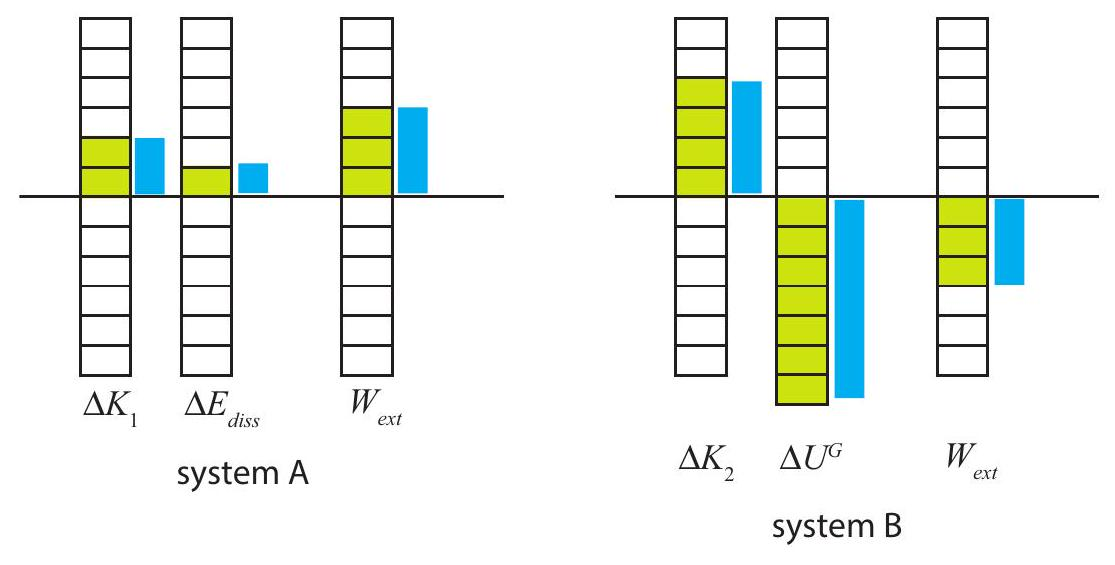
\includegraphics[max width=\textwidth]{2024_09_14_9969b06773f10b6936e8g-173}
\end{center}

\subsection*{7.7.3 Work, energy and the choice of system: non-dissipative case}
Suppose you hang a spring from the ceiling, then attach a block to the end of the spring and let go. The block starts swinging up and down on the spring. Consider the initial time just before you let go, and the final time when the block momentarily stops at the bottom of the swing. For each of the choices of a system listed below, find the net energy change of the system in this process, and relate it explicitly to the work done on the system by an external force (or forces)\\
(a) System is the block and the spring.\\
(b) System is the block alone.\\
(c) System is the block and the earth.

\section*{Solution}
(a) The block alone has kinetic energy, and the spring alone has (elastic) potential energy, so the total energy of this system is the sum of these two. For the interval considered, the change in kinetic energy is zero, because the block starts and ends (momentarily) at rest, so only the spring energy changes. This has to be equal to the work done by gravity, which is the only external force.

So, if the spring stretches a distance $d$, its potential energy goes from zero to $\frac{1}{2} k d^{2}$, and the block falls the same distance, so gravity does an amount of work equal to $m g d$, and we have


\begin{equation*}
W_{\text {grav }}=m g d=\Delta E_{\text {sys }}=\Delta K+\Delta U^{s p r}=0+\frac{1}{2} k d^{2} \tag{7.41}
\end{equation*}


(b) If the system is the block alone, the only energy it has is kinetic energy, which, as stated above, does not see a net change in this process. This means the net work done on the block by the external forces must be zero. The external forces in this case are the spring force and gravity, so we have


\begin{equation*}
W_{\text {spr }}+W_{\text {grav }}=\Delta K=0 \tag{7.42}
\end{equation*}


We have calculated $W_{\text {grav }}$ above, so from this we get that the work done by the spring on the block, as it stretches, is $-m g d$, or (by Eq. (7.41)) $-\frac{1}{2} k d^{2}$. Note that the force exerted by the spring is not constant as it stretches (or compresses) so we cannot just use Eq. (7.4) to calculate it; rather, we need to calculate it as an integral, as in Eq. (7.9), or derive it in some indirect way as we have just done here.\\
(c) If the system is the block and the earth, it has kinetic energy and gravitational potential energy. The force exerted by the spring is an external force now, so we have:


\begin{equation*}
W_{s p r}=\Delta E_{s y s}=\Delta K+\Delta U^{G}=0-m g d \tag{7.43}
\end{equation*}


so we end up again with the result that $W_{\text {spr }}=-m g d=-\frac{1}{2} k d^{2}$. Note that both the work done by the spring and the work done by gravity are equal to the negative of the changes in their respective potential energies, as they should be.

\subsection*{7.7.4 Jumping}
For a standing jump, you start standing straight (A) so your body's center of mass is at a height $h_{1}$ above the ground. You then bend your knees so your center of mass is now at a (lower) height $h_{2}$ (B). Finally, you straighten your legs, pushing hard on the ground, and take off, so your center of mass ends up achieving a maximum height, $h_{3}$, above the ground (C). Answer the following questions in as much detail as you can.\\
(a) Consider the system to be your body only. In going from (A) to (B), which external forces are acting on it? How do their magnitudes compare, as a function of time?\\
(b) In going from (A) to (B), does any of the forces you identified in part (a) do work on your body? If so, which one, and by how much? Does your body's energy increase or decrease as a result of this? Into what kind of energy do you think this work is primarily converted?\\
(c) In going from (B) to (C), which external forces are acting on you? (Not all of them need to be acting all the time.) How do their magnitudes compare, as a function of time?\\
(d) In going from (B) to (C), does any of the forces you identified do work on your body? If so, which one, and by how much? Does your body's kinetic energy see a net change from (B) to (C)? What other energy change needs to take place in order for Eq. (7.20) (always with your body as the system) to be valid for this process?

\section*{Solution}
(a) The external forces on your body are gravity, pointing down, and the normal force from the floor, pointing up. Initially, as you start lowering your center of mass, the normal force has to be slightly smaller than gravity, since your center of mass acquires a small downward acceleration. However, eventually $F^{n}$ would have to exceed $F^{G}$ in order to stop the downward motion.\\
(b) The normal force does no work, because its point of application (the soles of your feet) does not move, so $\Delta x$ in the expression $W=F \Delta x$ (Eq. (7.4)) is zero.

Gravity, on the other hand, does positive work, since you may always treat the center of mass as the point of application of gravity (see Section 7.3 , footnote). We have $F_{y}^{G}=-m g$, and $\Delta y=h_{2}-h_{1}$, so

$$
W_{\text {grav }}=F_{y}^{G} \Delta y=-m g\left(h_{2}-h_{1}\right)=m g\left(h_{1}-h_{2}\right)
$$

Since this is the net work done by all the external forces on my body, and it is positive, the total energy in my body must have increased (by the theorem (7.20): $W_{\text {ext,sys }}=\Delta E_{\text {sys }}$ ). In this case, it is clear that the main change has to be an increase in my body's elastic potential energy, as my muscles tense for the jump. (An increase in thermal energy is always possible too.)\\
(c) During the jump, the external forces acting on me are again gravity and the normal force, which together determine the acceleration of my center of mass. At the beginning of the jump, the normal force has to be much stronger than gravity, to give me a large upwards acceleration. Since the normal force is a reaction force, I accomplish this by pushing very hard with my feet on the ground, as I extend my leg's muscles: by Newton's third law, the ground responds with an equal and opposite force upwards.

As my legs continue to stretch, and move upwards, the force they exert on the ground decreases, and so does $F^{n}$, which eventually becomes less than $F^{G}$. At that point (probably even before my feet leave the ground) the acceleration of my center of mass becomes negative (that is, pointing down). This ultimately causes my upwards motion to stop, and my body to come down.\\
(d) The only force that does work on my body during the process described in (c) is gravity, since, again, the point of application of $F^{n}$ is the point of contact between my feet and the ground, and that point does not move up or down - it is always level with the ground. So $W_{\text {ext,sys }}=W_{\text {grav }}$, which in this case is actually negative: $W_{\text {grav }}=-m g\left(h_{3}-h_{2}\right)$.

In going from (B) to (C), there is no change in your kinetic energy, since you start at rest and end (momentarily) with zero velocity at the top of the jump. So the fact that there is a net negative work done on you means that the energy inside your body must have gone down. Clearly, some of this is just a decrease in elastic potential energy. However, since $h_{3}$ (the final height of your center of mass) is greater than $h_{1}$ (its initial height at (A), before crouching), there is a net loss of energy in your body as a result of the whole process. The most obvious place to look for this loss is in chemical energy: you "burned" some calories in the process, primarily when pushing hard against the ground.

\subsection*{7.8 Problems}
Problem 1 In a mattress test, you drop a 7.0 kg bowling ball from a height of 1.5 m above a mattress, which as a result compresses 15 cm as the ball comes to a stop.\\
(a) What is the kinetic energy of the ball just before it hits the mattress?\\
(b) How much work does the gravitational force of the earth do on the ball as it falls, for the first part of the fall (from the moment you drop it to just before it hits the mattress)?\\
(c) How much work does the gravitational force do on the ball while it is compressing the mattress?\\
(d) How much work does the mattress do on the ball?\\
(e) Now model the mattress as a single spring with an unknown spring constant $k$, and consider the whole system formed by the ball, the earth and the mattress. By how much does the potential energy of the mattress increase as it compresses?\\
(f) What is the value of the spring constant $k$ ?

Problem 2 A block of mass 1 kg is sitting on top of a compressed spring of spring constant $k=300 \mathrm{~N} / \mathrm{m}$ and equilibrium length 20 cm . Initially the spring is compressed 10 cm , and the block is held in place by someone pushing down on it with his hand. At $t=0$, the hand is removed (this involves no work), the spring expands and the block flies upwards.\\
(a) Draw a free-body diagram for the block while the hand is still pressing down. Try to get the forces approximately to scale. The following question should help.\\
(b) What must be the force (magnitude and direction) exerted by the hand on the block?\\
(c) How much elastic potential energy was stored in the spring initially?\\
(d) Taking the system formed by the block and the earth, how much total work is done on it by the spring, as it expands to its equilibrium length? (You do not need to do a new calculation here, just think of conservation of energy.)\\
(e) How high does the block rise above its initial position?\\
(f) Treating the block alone as the system, how much net work is done on it by the two external forces (the spring and gravity) from the time just before it starts moving to the time it reaches its maximum height? (Again, no calculation is necessary if you can justify your answer.)

Problem 3 A crane is lifting a $500-\mathrm{kg}$ object at a constant speed of $0.5 \mathrm{~m} / \mathrm{s}$. What is the power output of the crane?

Problem 4 In a crash test, a car, initially moving at $30 \mathrm{~m} / \mathrm{s}$, hits a wall and crumples to a halt. In the process of crumpling, the center of mass of the car moves forward a distance of 1 m .\\
(a) If the car has a mass of $1,800 \mathrm{~kg}$, what is the magnitude of the average force acting on it while it stops? What, physically, is this force?\\
(b) Does the force you found in (a) actually do any work on the car? (Think carefully!)\\
(c) What is the net change in the car's kinetic energy? Where does all that kinetic energy go?

Problem 5 A block of mass 3 kg slides on a horizontal, rough surface towards a spring with $k=500 \mathrm{~N} / \mathrm{m}$. The kinetic friction coefficient between the block and the surface is $\mu_{k}=0.6$. If the block's speed is $5 \mathrm{~m} / \mathrm{s}$ at the instant it first makes contact with the spring,\\
(a) Find the maximum compression of the spring.\\
(b) Draw work-energy bar diagrams for the process of the block coming to a halt, taking the system to be the block and the surface only.

\section*{Chapter 8}
\section*{Motion in two dimensions}
\subsection*{8.1 Dealing with forces in two dimensions}
We have been able to get a lot of physics from our study of (mostly) one-dimensional motion only, but it goes without saying that the real world is a lot richer than that, and there are a number of new and interesting phenomena that appear when one considers motion in two or three dimensions. The purpose of this chapter is to introduce you to some of the simplest two-dimensional situations of physical interest.

A common feature to all these problems is that the forces acting on the objects under consideration will typically not line up with the displacements. This means, in practice, that we need to pay more attention to the vector nature of these quantities than we have done so far. This section will present a brief reminder of some basic properties of vectors, and introduce a couple of simple principles for the analysis of the systems that will follow.

To begin with, recall that a vector is a quantity that has both a magnitude and a direction. The magnitude of the vector just tells us how big it is: the magnitude of the velocity vector, for instance, is the speed, that is, just how fast something is moving. When working with vectors in one dimension, we have typically assumed that the entire vector (whether it was a velocity, an acceleration or a force) lay along the line of motion of the system, and all we had to do to indicate the direction was to give the vector's magnitude an appropriate sign. For the problems that follow, however, it will become essential to break up the vectors into their components along an appropriate set of axes. This involves very simple geometry, and follows the example of the position vector $\vec{r}$, whose components are just the Cartesian coordinates of the point it locates in space (as shown in Figure 1.1). For a generic vector, for instance, a force, like the one shown in Figure 8.1 below, the components $F_{x}$ and $F_{y}$ may be obtained from a right triangle, as indicated there:

\begin{center}
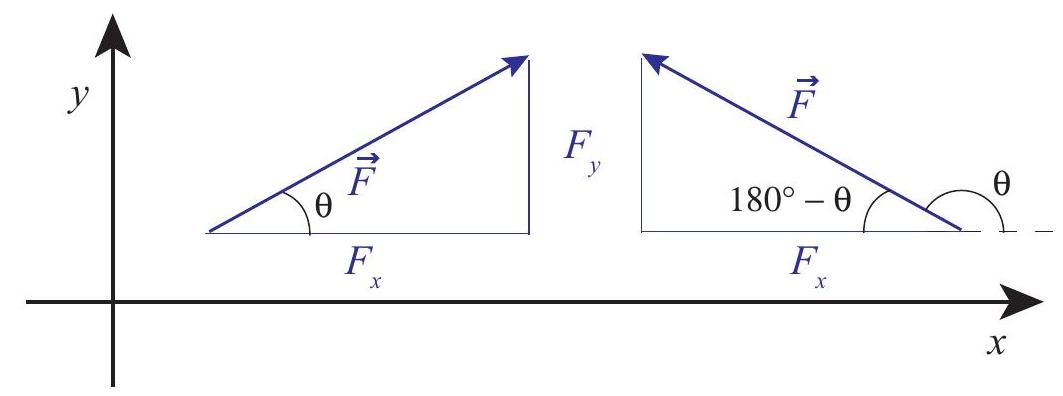
\includegraphics[max width=\textwidth]{2024_09_14_9969b06773f10b6936e8g-180}
\end{center}

Figure 8.1: The components of a vector that makes an angle $\theta$ with the positive $x$ axis. Two examples are shown, for $\theta<90^{\circ}$ (in which case $F_{x}>0$ ) and for $90^{\circ}<\theta<180^{\circ}$ (in which case $F_{x}<0$ ). In both cases, $F_{y}>0$.

The triangle will always have the vector's magnitude $(|\vec{F}|$ in this case $)$ as the hypothenuse. The two other sides should be parallel to the coordinate axes. Their lengths are the corresponding components, except for a sign that depends on the orientation of the vector. If we happen to know the angle $\theta$ that the vector makes with the positive $x$ axis, the following relations will always hold:


\begin{align*}
F_{x} & =|\vec{F}| \cos \theta \\
F_{y} & =|\vec{F}| \sin \theta \\
|\vec{F}| & =\sqrt{F_{x}^{2}+F_{y}^{2}} \\
\theta & =\tan ^{-1} \frac{F_{y}}{F_{x}} \tag{8.1}
\end{align*}


Note, however, that in general this angle $\theta$ may not be one of the interior angles of the triangle (as shown on the right diagram in Fig. 8.1), and that in that case it may just be simpler to calculate the magnitude of the components using trigonometry and an interior angle (such as $180^{\circ}-\theta$ in the example), and give them the appropriate signs "by hand." In the example on the right, the length of the horizontal side of the triangle is equal to $|\vec{F}| \cos \left(180^{\circ}-\theta\right)$, which is a positive quantity; the correct value for $F_{x}$, however, is the negative number $|\vec{F}| \cos \theta=-|\vec{F}| \cos \left(180^{\circ}-\theta\right)$.

In any case, it is important not to get fixated on the notion that "the $x$ component will always be proportional to the cosine of $\theta$." The symbol $\theta$ is just a convenient one to use for a generic angle. There are four sections in this chapter, and in every one there is a $\theta$ used with a different meaning. When in doubt, just draw the appropriate right triangle and remember from your trigonometry classes which side goes with the sine, and which with the cosine.

For the problems that we are going to study in this chapter, the idea is to break up all the forces involved into components along properly-chosen coordinate axes, then add all the components along any given direction, and apply $F_{n e t}=m a$ along that direction: that is to say, we will write (and\\
eventually solve) the equations


\begin{align*}
F_{n e t, x} & =m a_{x} \\
F_{n e t, y} & =m a_{y} \tag{8.2}
\end{align*}


We can show that Eqs. (8.2) must hold for any choice of orthogonal $x$ and $y$ axes, based on the fact that we know $\vec{F}_{\text {net }}=m \vec{a}$ holds along one particular direction, namely, the direction common to $\vec{F}_{n e t}$ and $\vec{a}$, and the fact that we have defined the projection procedure to be the same for any kind of vector. Figure 8.2 shows how this works. Along the dashed line you just have the situation that is by now familiar to us from one-dimensional problems, where $\vec{a}$ lies along $\vec{F}$ (assumed here to be the net force), and $|\vec{F}|=m|\vec{a}|$. However, in the figure I have chosen the axes to make an angle $\theta$ with this direction. Then, if you look at the projections of $\vec{F}$ and $\vec{a}$ along the $x$ axis, you will find


\begin{align*}
& a_{x}=|\vec{a}| \cos \theta \\
& F_{x}=|\vec{F}| \cos \theta=m|\vec{a}| \cos \theta=m a_{x} \tag{8.3}
\end{align*}


and similarly, $F_{y}=m a_{y}$. In words, each component of the force vector is responsible for only the corresponding component of the acceleration. A force in the $x$ direction does not cause any acceleration in the $y$ direction, and vice-versa.

\begin{center}
\includegraphics[max width=\textwidth]{2024_09_14_9969b06773f10b6936e8g-181}
\end{center}

Figure 8.2: If you take the familiar, one-dimensional (see the black dashed line) form of $\vec{F}=m \vec{a}$, and project it onto orthogonal, rotated axes, you get the general two-dimensional case, showing that each orthogonal component of the acceleration is proportional, via the mass $m$, to only the corresponding component of the force (Eqs. (8.2)).

In the rest of the chapter we shall see how to use Eqs. (8.2) in a number of examples. One thing I can anticipate is that, in general, we will try to choose our axes (unlike in Fig. 8.2 above) so that one of them does coincide with the direction of the acceleration, so the motion along the other direction is either nonexistent $(v=0)$ or trivial (constant velocity).

\subsection*{8.2 Projectile motion}
Projectile motion is basically just free fall, only with the understanding that the object we are tracking was "projected," or "shot," with some initial velocity (as opposed to just dropped from rest). Unlike in the previous cases of free fall that we have studied so far, we will now assume that the initial velocity has a horizontal component, as a result of which, instead of just going straight up and/or down, the object will describe (ignoring air resistance, as usual) a parabola in a vertical plane.

The plane in question is determined by the initial velocity (more precisely, the horizontal component of the initial velocity) and gravity. A generic trajectory is shown in Figure 8.3, showing the force and acceleration vectors (constant throughout) and the velocity vector at various points along the path.

\begin{center}
\includegraphics[max width=\textwidth]{2024_09_14_9969b06773f10b6936e8g-182}
\end{center}

Figure 8.3: A typical projectile trajectory. The velocity vector (in green) is shown at the initial time, the point of maximum height, and the point where the projectile is back to its initial height.

Conceptually, the problem turns out to be extremely simple if we apply the basic principle introduced in Section 8.1. The force is vertical throughout; so, after the throw, there is no horizontal acceleration, and the vertical acceleration is just $-g$, just as it always was in our earlier, onedimensional free-fall problems:


\begin{align*}
& a_{x}=\frac{F_{x}}{m}=0 \\
& a_{y}=\frac{F_{y}}{m}=-g \tag{8.4}
\end{align*}


The overall motion, then, is a combination of motion with constant velocity horizontally, and motion with constant acceleration vertically, and we can write down the corresponding equations of motion immediately:


\begin{align*}
v_{x} & =v_{x, i} \\
v_{y} & =v_{y, i}-g t \\
x & =x_{i}+v_{x, i} t \\
y & =y_{i}+v_{y, i} t-\frac{1}{2} g t^{2} \tag{8.5}
\end{align*}


where $\left(x_{i}, y_{i}\right)$ are the coordinates of the launching point (there is usually no reason to make $x_{i}$ anything other than zero, so we will do that below), and $\left(v_{x, i}, v_{y, i}\right)$ the initial components of the velocity vector.

By eliminating $t$ in between the last two Eqs. (8.5), we get the equation of the trajectory in the $x-y$ plane:


\begin{equation*}
y=y_{i}+\frac{v_{y, i}}{v_{x, i}} x-\frac{g}{2 v_{x, i}^{2}} x^{2} \tag{8.6}
\end{equation*}


which, as indicated earlier, and as shown in Fig. 8.3, is indeed the equation of a parabola.\\
The apex of the parabola (highest point in the trajectory) is at $x_{\text {max height }}=v_{x, i} v_{y, i} / g$. We can get this result from calculus, or from a comparison of Eq. (8.6) with the canonical form of a parabola, or we can use some physics: the maximum height is reached, as usual, when the vertical velocity becomes momentarily zero, so solving the $v_{y}$ equation (8.5) for $t_{\text {max }}$ height and substituting in the $x$ equation, we get


\begin{align*}
t_{\text {max height }} & =\frac{v_{y, i}}{g} \\
x_{\text {max height }} & =\frac{v_{x, i} v_{y, i}}{g} \\
y_{\text {max height }} & =y_{i}+\frac{v_{y, i}^{2}}{2 g} \tag{8.7}
\end{align*}


The last of these equations should look familiar. It is, indeed a variation on our old friend $v_{f}^{2}-v_{i}^{2}=$ $-2 g \Delta y$, only now instead of the full velocity $\vec{v}$ we have to use only the vertical velocity component $v_{y}$. Just like for one-dimensional motion, this result follows again from conservation of energy: throughout the flight, we must have $K+U^{G}=$ constant, only now there is a component to the kinetic energy - the part associated with the horizontal motion - which remains constant on its own. In general, the kinetic energy of a particle will be $\frac{1}{2} m|\vec{v}|^{2}$, where $|\vec{v}|$ is the magnitude of the velocity vector - that is to say, the speed. In two dimensions, this gives


\begin{equation*}
K=\frac{1}{2} m v_{x}^{2}+\frac{1}{2} m v_{y}^{2} \tag{8.8}
\end{equation*}


For projectile motion, however, $v_{x}$ does not change, so any change in $K$ will affect only the second term in Eq. (8.8). Conservation of energy between any two instants $i$ and $f$ gives


\begin{equation*}
K+U^{G}=\frac{1}{2} m v_{x, i}^{2}+\frac{1}{2} m v_{y, i}^{2}+m g y_{i}=\frac{1}{2} m v_{x, i}^{2}+\frac{1}{2} m v_{y, f}^{2}+m g y_{f} \tag{8.9}
\end{equation*}


The $\frac{1}{2} m v_{x, i}^{2}$ term cancels, and therefore


\begin{equation*}
v_{y, f}^{2}-v_{y, i}^{2}=-2 g\left(y_{f}-y_{i}\right) \tag{8.10}
\end{equation*}


Another quantity of interest is the projectile's range, or maximum horizontal distance traveled. We can calculate it from Eqs. (8.5), by setting $y$ equal to the final height, then solving for $t$ (which generally requires solving a quadratic equation), and then substituting the result in the equation for $x$. In the simple case when the final height is the same as the initial height, we can avoid the need for calculating altogether, and just reason, from the fact that the trajectory is symmetric, that the total horizontal distance traveled will be twice the distance to the point where the maximum height is reached, that is, $x_{\text {range }}=2 x_{\text {max height }}$ :


\begin{equation*}
x_{\text {range }}=\frac{2 v_{x, i} v_{y, i}}{g} \quad\left(\text { only if } y_{f}=y_{i}\right) \tag{8.11}
\end{equation*}


As you can see, all these equations depend on the initial values of the components of the velocity vector $\vec{v}_{i}$. If $\vec{v}_{i}$ makes an angle $\theta$ with the horizontal, and we simplify the notation by calling its magnitude $v_{i}$, then we can write


\begin{align*}
& v_{x, i}=v_{i} \cos \theta \\
& v_{y, i}=v_{i} \sin \theta \tag{8.12}
\end{align*}


In terms of $v_{i}$ and $\theta$, the range equation (8.11) becomes


\begin{equation*}
x_{\text {range }}=\frac{v_{i}^{2} \sin (2 \theta)}{g} \quad\left(\text { only if } y_{f}=y_{i}\right) \tag{8.13}
\end{equation*}


since $2 \sin \theta \cos \theta=\sin (2 \theta)$. This tells us that for any given launch speed, the maximum range is achieved when the launch angle $\theta=45^{\circ}$ (always assuming the final height is the same as the initial height).

In real life, of course, there will always be air resistance, and all these results will be modified somewhat. Mathematically, things become a lot more complicated: the drag force depends on the speed, which involves both components of the velocity, so the horizontal and vertical motions are no longer decoupled: not only is there now an $F_{x}$, but its value at any given time depends both on $v_{x}$ and $v_{y}$. Physically, you may think of the drag force as doing negative work on the projectile, and hence removing kinetic energy from it. Less kinetic energy means, basically, that it will not travel quite as far either vertically or horizontally. Surprisingly, the optimum launch angle remains pretty close to $45^{\circ}$, at least if the simulations at this link are accurate:\\
\href{https://phet.colorado.edu/en/simulation/projectile-motion}{https://phet.colorado.edu/en/simulation/projectile-motion}

\subsection*{8.3 Inclined planes}
Back in Chapter 2, I stated without proof that the acceleration of an object sliding, without friction, down an inclined plane making an angle $\theta$ with the horizontal was $g \sin \theta$. I can show you now why this is so, and introduce friction as well.\\
\includegraphics[max width=\textwidth, center]{2024_09_14_9969b06773f10b6936e8g-185}

Figure 8.4: A block sliding down an inclined plane. The corresponding free-body diagram is shown on the right.

Figure 8.4 above shows, on the left, a block sliding down an inclined plane and all the forces acting on it. These are more clearly seen on the free-body diagram on the right. I have labeled all the forces using the $\vec{F}_{b y, o n}^{\text {type }}$ convention introduced back in Chapter 6 (so, for instance, $\vec{F}_{s b}^{k}$ is the force of kinetic friction exerted by the surface on the block); however, later on, for algebraic manipulations, and especially where $x$ and $y$ components need to be taken, I will drop the "by, on" subscripts, and just let the "type" superscript identify the force in question.

The diagrams also show the coordinate axes I have chosen: the $x$ axis is along the plane, and the $y$ is perpendicular to it. The advantage of this choice is obvious: the motion is entirely along one of the axes, and two of the forces (the normal force and the friction) already lie along the axes. The only force that does not is the block's weight (that is, the force of gravity), so we need to decompose it into its $x$ and $y$ components. For this, we can make use of the fact, which follows from basic geometry, that the angle of the incline, $\theta$, is also the angle between the vector $\vec{F}^{g}$ and the negative $y$ axis. This means we have


\begin{align*}
& F_{x}^{g}=F^{g} \sin \theta \\
& F_{y}^{g}=-F^{g} \cos \theta \tag{8.14}
\end{align*}


Equations (8.14) also show another convention I will adopt from now, namely, that whenever the symbol for a vector is shown without an arrow on top or an $x$ or $y$ subscript, it will be understood to refer to the magnitude of the vector, which is always a positive number by definition.

Newton's second law, as given by equations (8.4) applied to this system, then reads:


\begin{equation*}
F_{x}^{g}+F_{x}^{k}=m a_{x}=F^{g} \sin \theta-F^{k} \tag{8.15}
\end{equation*}


for the motion along the plane, and


\begin{equation*}
F_{y}^{g}+F_{y}^{n}=m a_{y}=-F^{g} \cos \theta+F^{n} \tag{8.16}
\end{equation*}


for the direction perpendicular to the plane. Of course, since there is no motion in this direction, $a_{y}$ is zero. This gives us immediately the value of the normal force:


\begin{equation*}
F^{n}=F^{g} \cos \theta=m g \cos \theta \tag{8.17}
\end{equation*}


since $F^{g}=m g$. We can also use the result (8.17), together with Eq. (6.30), to get the magnitude of the friction force, assuming we know the coefficient of kinetic (or sliding) friction, $\mu_{k}$ :


\begin{equation*}
F^{k}=\mu_{k} F^{n}=\mu_{k} m g \cos \theta \tag{8.18}
\end{equation*}


Substituting this and $F^{g}=m g$ in Eq. (8.15), we get


\begin{equation*}
m a_{x}=m g \sin \theta-\mu_{k} m g \cos \theta \tag{8.19}
\end{equation*}


We can eliminate the mass to obtain finally


\begin{equation*}
a_{x}=g\left(\sin \theta-\mu_{k} \cos \theta\right) \tag{8.20}
\end{equation*}


which is the desired result. In the absence of friction $\left(\mu_{k}=0\right)$ this gives $a=g \sin \theta$, as we had in Chapter 2. Note that, if you reduce the tilt of the surface (that is, make $\theta$ smaller), the $\cos \theta$ term in Eq. (8.20) grows and the $\sin \theta$ term gets smaller, so we must make sure that we do not use this equation when $\theta$ is too small or we would get the absurd result that $a_{x}<0$, that is, that the force of kinetic friction has overcome gravity and is accelerating the object upwards!

Of course, we know from experience that what happens when $\theta$ is very small is that the block does not slide: it is held in place by the force of static friction. The diagram for such a situation looks the same as Fig. 8.4, except that $\vec{a}=0$, the force of friction is $F^{s}$ instead of $F^{k}$, and of course its magnitude must match that of the $x$ component of gravity. Equation (8.15) then becomes


\begin{equation*}
m a_{x}=0=F^{g} \sin \theta-F^{s} \tag{8.21}
\end{equation*}


Recall from Chapter 6 that the force of static friction does not have a fixed value: rather, it will match the applied force up to a maximum value given by Eq. (6.29):


\begin{equation*}
F_{\max }^{s}=\mu_{s} F^{n}=\mu_{s} m g \cos \theta \tag{8.22}
\end{equation*}


where I have used Eq. (8.17), since clearly the equation (8.16) still applies along the vertical direction. So, on the one hand we have the requirement that $F^{s}=m g \sin \theta$ to keep the block from\\
sliding, and on the other hand the constraint $F^{s} \leq \mu_{s} m g \cos \theta$. Putting these together we conclude that the block will not slide as long as


\begin{equation*}
m g \sin \theta \leq \mu_{s} m g \cos \theta \tag{8.23}
\end{equation*}


or


\begin{equation*}
\tan \theta \leq \mu_{s} \tag{8.24}
\end{equation*}


In short, as long as $\theta$ is small enough to satisfy Eq. (8.24), the block will not move. Once $\theta$ exceeds the value $\tan ^{-1} \mu_{s}$, we can apply the result (8.20) for the acceleration. Note that, since we always have $\mu_{s} \geq \mu_{k}$, the result (8.20) will always be positive if $\theta>\tan ^{-1} \mu_{s}$, that is, if $\sin \theta>\mu_{s} \cos \theta$.

What if we send the block sliding $u p$ the plane instead? The acceleration would still be pointing down (since the object would be slowing down all the while), but now the force of kinetic friction would point in the direction opposite that indicated in Figure 8.4, since it always must oppose the motion. If you go through the same analysis I carried out above, you will get that $a_{x}=$ $g\left(\sin \theta+\mu_{k} \cos \theta\right)$ in that case, since now friction and gravity are working together to slow the motion down.

\subsection*{8.4 Motion on a circle (or part of a circle)}
The last example of motion in two dimensions that I will consider in this chapter is motion on a circle. There are many examples of circular (or near-circular) motion in nature, particularly in astronomy (as we shall see in a later chapter, the orbits of most planets and many satellites are very nearly circular). There are also many devices that we use all the time that involve rotating or spinning objects (wheels, gears, turntables, turbines...). All of these can be mathematically described as collections of particles moving in circles.

In this section, I will first introduce the concept of centripetal force, which is the force needed to bend an object's trajectory into a circle (or an arc of a circle), and then I will also introduce a number of quantities that are useful for the description of circular motion in general, such as angular velocity and angular acceleration. The dynamics of rotational motion (questions having to do with rotational energy, and a new important quantity, angular momentum) will be the subject of the next chapter.

\subsection*{8.4.1 Centripetal acceleration and centripetal force}
As you know by now, the law of inertia states that, in the absence of external forces, an object will move with constant speed on a straight line. A circle is not a straight line, so an object will not naturally follow a circular path unless there is a force acting on it.

Another way to see this is to go back to the definition of acceleration. If an object has a velocity vector $\vec{v}(t)$ at the time $t$, and a different velocity vector $\vec{v}(t+\Delta t)$ at the later time $t+\Delta t$, then its average acceleration over the time interval $\Delta t$ is the quantity $\vec{v}_{a v}=(\vec{v}(t+\Delta t)-\vec{v}(t)) / \Delta t$. This is nonzero even if the speed does not change (that is, even if the two velocity vectors have the same magnitude), as long as they have different directions, as you can see from Figure 8.5 below. Thus, motion on a circle (or an arc of a circle), even at constant speed, is accelerated motion, and, by Newton's second law, accelerated motion requires a force to make it happen.\\
\includegraphics[max width=\textwidth, center]{2024_09_14_9969b06773f10b6936e8g-188}

Figure 8.5: A particle moving along an arc of a circle of radius $R$. The positions and velocities at the times $t$ and $t+\Delta t$ are shown. The diagram on the right shows the velocity difference, $\Delta \vec{v}=\vec{v}(t+\Delta t)-\vec{v}(t)$.

We can find out how large this acceleration, and the associated force, have to be, by applying a little geometry and trigonometry to the situation depicted in Figure 8.5. Here a particle is moving along an arc of a circle of radius $r$, so that at the time $t$ it is at point P and at the later time $t+\Delta t$ it is at point Q . The length of the arc between P and Q (the distance it has traveled) is $s=R \theta$, where the angle $\theta$ is understood to be in radians. I have assumed the speed to be constant, so the magnitude of the velocity vector, $v$, is just equal to the ratio of the distance traveled (along the circle), to the time elapsed: $v=s / \Delta t$.

Despite the speed being constant, the motion is accelerated, as I just said above, because the direction of the velocity vector changes. The diagram on the right shows the velocity difference vector $\Delta \vec{v}=\vec{v}(t+\Delta t)-\vec{v}(t)$. We can get its length from trigonometry: if we split the angle $\theta$ in half, we get two right triangles, and for each of them $|\Delta \vec{v}| / 2=v \sin (\theta / 2)$. Thus, we have


\begin{equation*}
\left|\vec{a}_{a v}\right|=\frac{|\Delta \vec{v}|}{\Delta t}=\frac{2 v \sin (\theta / 2)}{\Delta t} \tag{8.25}
\end{equation*}


for the magnitude of the average acceleration vector. The instantaneous acceleration is obtained by taking the limit of this expression as $\Delta t \rightarrow 0$. In this limit, the angle $\theta=s / R=v \Delta t / R$ becomes\\
very small, and we can use the so-called "small angle approximation," which states that $\sin x \simeq x$ when $x$ is small and expressed in radians. Therefore, by Eq. (8.25),


\begin{equation*}
\left|\vec{a}_{a v}\right|=\frac{2 v \sin (\theta / 2)}{\Delta t} \simeq \frac{v \theta}{\Delta t}=\frac{v^{2} \Delta t / R}{\Delta t} \tag{8.26}
\end{equation*}


This expression becomes exact as $\Delta t \rightarrow 0$, and then $\Delta t$ cancels out, showing the instantaneous acceleration has magnitude


\begin{equation*}
|\vec{a}|=a_{c}=\frac{v^{2}}{R} \tag{8.27}
\end{equation*}


This acceleration is called the centripetal acceleration, which is why I have denoted it by the symbol $a_{c}$. The reason for that name is that it is always pointing towards the center of the circle. You can kind of see this from Figure 8.5: if you take the vector $\Delta \vec{v}$ shown there, and move it (without changing its direction, so it stays 'parallel to itself") to the midpoint of the arc, halfway between points P and Q, you will see that it does point almost straight to the center of the circle. (A more mathematically rigorous proof of this fact, using calculus, will be presented in the next chapter, section 9.3.)

The force $\vec{F}_{c}$ needed to provide this acceleration is called the centripetal force, and by Newton's second law it has to satisfy $\vec{F}_{c}=m \vec{a}_{c}$. Thus, the centripetal force has magnitude


\begin{equation*}
F_{c}=m a_{c}=\frac{m v^{2}}{R} \tag{8.28}
\end{equation*}


and, like the acceleration $\vec{a}_{c}$, is always directed towards the center of the circle.\\
Physically, the centripetal force $F_{c}$, as given by Eq. (8.28), is what it takes to bend the trajectory so as to keep it precisely on an arc of a circle of radius $R$ and with constant speed $v$. Note that, since $\vec{F}_{c}$ is always perpendicular to the displacement (which, over any short time interval, is essentially tangent to the circle), it does no work on the object, and therefore (by Eq. (7.11)) its kinetic energy does not change, so $v$ does indeed stay constant when the centripetal force equals the net force. Note also that "centripetal" is just a job description: it is not a new type of force. In any given situation, the role of the centripetal force will be played by one of the forces we are already familiar with, such as the tension on a rope (or an appropriate component thereof) when you are swinging an object in a horizontal circle, or gravity in the case of the moon or any other satellite.

At this point, if you have never heard about the centripetal force before, you may be feeling a little confused, since you almost certainly have heard, instead, about a so-called centrifugal force that tends to push spinning things away from the center of rotation. In fact, however, this "centrifugal force" does not really exist: the "force" that you may feel pushing you towards the outside of a curve when you ride in a vehicle that makes a sharp turn is really nothing but your own inertia-your body "wants" to keep moving on a straight line, but the car, by bending its trajectory, is preventing it from doing so. The impression that you get that you would fly radially out, as opposed to along a tangent, is also entirely due to the fact that the reference frame you are in (the car) is continuously\\
changing its direction of motion. You will find this effect illustrated in some detail in an example in the "Advanced Topics" section, if you want to look at it in more depth.

On the other hand, getting a car to safely negotiate a turn is actually an important example of a situation that requires a definite centripetal force. On a flat surface (see the "Advanced Topics" section for a treatment of a banked curve!), you rely entirely on the force of static friction to keep you on the track, which can typically be modeled as an arc of a circle with some radius $R$. So, if you are traveling at a speed $v$, you need $F^{s}=m v^{2} / R$. Recalling that the force of static friction cannot exceed $\mu_{s} F^{n}$, and that on a flat surface you would just have $F^{n}=F^{g}=m g$, you see you need to keep $m v^{2} / R$ smaller than $\mu_{s} m g$; or, canceling the mass,


\begin{equation*}
\frac{v^{2}}{R}<\mu_{s} g \tag{8.29}
\end{equation*}


This is the condition that has to hold in order to be able to make the turn safely. The maximum speed is then $v_{\max }=\sqrt{\mu_{s} g R}$, which, as you can see, will depend on the state of the road (for instance, if the road is wet the coefficient $\mu_{s}$ will be smaller). The posted, recommended speed will typically take this into consideration and will be as low as it has to be to keep you safe. Notice that the left-hand side of Eq. (8.29) increases as the square of the speed, so doubling your speed makes that term four times larger! Do not even think of taking a turn at 60 mph if the recommended speed is 30 , and do not exceed the recommended speed at all if the road is wet or your tires are worn.

\subsection*{8.4.2 Kinematic angular variables}
Consider a particle moving on a circle, as in Figure 8.6 below (next page). Of course, we can just use the regular, cartesian coordinates, $x$ and $y$, to describe its motion. But, in a way, this is carrying around more information than we typically need, and it is also not very transparent: a value of $x$ and $y$ does not immediately tell us how far the object has traveled along the circle itself.

Instead, the most convenient way to describe the motion of the particle, if we know the radius of the circle, is to give the angle $\theta$ that the position vector makes with some reference axis at any given time, as shown in Fig. 8.6. If we choose the $x$ axis as the reference, then the conversion from a description based on the radius $R$ and the angle $\theta$ to a description in terms of $x$ and $y$ is simply


\begin{align*}
& x=R \cos \theta \\
& y=R \sin \theta \tag{8.30}
\end{align*}


so knowing the function $\theta(t)$ we can immediately get $x(t)$ and $y(t)$, if we need them. (Note: in this section I am using an uppercase $R$ for the magnitude of the position vector, to emphasize that it is a constant, equal to the radius of the circle.)

\begin{center}
\includegraphics[max width=\textwidth]{2024_09_14_9969b06773f10b6936e8g-191}
\end{center}

Figure 8.6: A particle moving on a circle. The position vector has length $R$, so the $x$ and $y$ coordinates are $R \cos \theta$ and $R \sin \theta$, respectively. The conventional positive direction of motion is indicated. The velocity vector is always, as usual, tangent to the trajectory.

Although the angle $\theta$ itself is not a vector quantity, nor a component of a vector, it is convenient to allow for the possibility that it might be negative. The standard convention is that $\theta$ grows in the counterclockwise direction from the reference axis, and decreases in the clockwise direction. Of course, you can always get to any angle by coming from either direction, so the angle by itself does not tell you how the particle got there. Information on the direction of motion at any given time is best captured by the concept of the angular velocity, which we represent by the symbol $\omega$ and define in a manner analogous to the way we defined the ordinary velocity: if $\Delta \theta=\theta(t+\Delta t)-\theta(t)$ is the angular displacement over a time $\Delta t$, then


\begin{equation*}
\omega=\lim _{\Delta t \rightarrow 0} \frac{\Delta \theta}{\Delta t}=\frac{d \theta}{d t} \tag{8.31}
\end{equation*}


The standard convention is also to use radians as an angle measure in this context, so that the units of $\omega$ will be radians per second, or $\mathrm{rad} / \mathrm{s}$. Note that the radian is a dimensionless unit, so it "disappears" from a calculation when the final result does not call for it (as in Eq. (8.35) below).

For motion with constant angular velocity, we clearly will have


\begin{equation*}
\theta(t)=\theta_{i}+\omega\left(t-t_{i}\right) \quad \text { or } \quad \Delta \theta=\omega \Delta t \quad(\text { constant } \omega) \tag{8.32}
\end{equation*}


where $\omega$ is positive for counterclockwise motion, and negative for clockwise. (There is a sense in which it is useful to think of $\omega$ as a vector, but, since it is not immediately obvious how or why, I will postpone discussion of this next chapter, after I have introduced angular momentum.)

When $\omega$ changes with time, we can introduce an angular acceleration $\alpha$, defined, again, in the obvious way:


\begin{equation*}
\alpha=\lim _{\Delta t \rightarrow 0} \frac{\Delta \omega}{\Delta t}=\frac{d \omega}{d t} \tag{8.33}
\end{equation*}


Then for motion with constant angular acceleration we have the formulas


\begin{align*}
& \omega(t)=\omega_{i}+\alpha\left(t-t_{i}\right) \quad \text { or } \quad \Delta \omega=\alpha \Delta t \quad(\text { constant } \alpha) \\
& \theta(t)=\theta_{i}+\omega_{i}\left(t-t_{i}\right)+\frac{1}{2} \alpha\left(t-t_{i}\right)^{2} \quad \text { or } \quad \Delta \theta=\omega_{i} \Delta t+\frac{1}{2} \alpha(\Delta t)^{2} \quad(\text { constant } \alpha) \tag{8.34}
\end{align*}


Equations (8.32) and (8.34) completely parallel the corresponding equations for motion in one dimension that we saw in Chapter 1. In fact, of course, a circle is just a line that has been bent in a uniform way, so the distance traveled along the circle itself is simply proportional to the angle swept by the position vector $\vec{r}$. As already pointed out in connection with Fig. 8.5, if we expressed $\theta$ in radians then the length of the arc corresponding to an angular displacement $\Delta \theta$ would be


\begin{equation*}
s=R|\Delta \theta| \tag{8.35}
\end{equation*}


so multiplying Eqs. (8.32) or (8.34) by $R$ directly gives the distance traveled along the circle in each case.

\begin{center}
\includegraphics[max width=\textwidth]{2024_09_14_9969b06773f10b6936e8g-192}
\end{center}

Figure 8.7: A small angular displacement. The distance traveled along the circle, $s=R \Delta \theta$, is almost identical to the straight-line distance $|\Delta \vec{r}|$ between the initial and final positions; the two quantities become the same in the limit $\Delta t \rightarrow 0$.

Figure 8.7 shows that, for very small angular displacements, it does not matter whether the distance traveled is measured along the circle itself or on a straight line; that is, $s \simeq|\Delta \vec{r}|$. Dividing by $\Delta t$, using Eq. (8.35) and taking the $\Delta t \rightarrow 0$ limit we get the following useful relationship between the angular velocity and the instantaneous speed $v$ (defined in the ordinary way as the distance traveled per unit time, or the magnitude of the velocity vector):


\begin{equation*}
|\vec{v}|=R|\omega| \tag{8.36}
\end{equation*}


As we shall see later, the product $R \alpha$ is also a useful quantity. It is not, however, equal to the magnitude of the acceleration vector, but only one of its two components, the tangential acceleration:


\begin{equation*}
a_{t}=R \alpha \tag{8.37}
\end{equation*}


The sign convention here is that a positive $a_{t}$ represents a vector that is tangent to the circle and points in the direction of increasing $\theta$ (that is, counterclockwise); the full acceleration vector is equal to the sum of this vector and the centripetal acceleration vector, introduced in the previous subsection, which always points towards the center of the circle and has magnitude


\begin{equation*}
a_{c}=\frac{v^{2}}{R}=R \omega^{2} \tag{8.38}
\end{equation*}


(making use of Eqs. (8.29) and (8.36)). These results will be formally established in the next chapter, after we introduce the vector product, although you could also verify them right now-if you are familiar enough with derivatives at this point - by using the chain rule to take the derivatives with respect to time of the components of the position vector, as given in Eq. (8.30) (with $\theta=\theta(t)$, an arbitrary function of time).

The main thing to remember about the radial and tangential components of the acceleration is that the radial component (the centripetal acceleration) is always there for circular motion, whether the angular velocity is constant or not, whereas the tangential acceleration is only nonzero if the angular velocity is changing, that is to say, if the particle is slowing down or speeding up as it turns.

\subsection*{8.5 In summary}
\begin{enumerate}
  \item To solve problems involving motion in two dimensions, you should break up all the forces into their components along a suitable pair of orthogonal axes, then apply Newton's second law to each direction separately: $F_{n e t, x}=m a_{x}, F_{n e t, y}=m a_{y}$. It is convenient to choose your axes so that at least one of either $a_{x}$ or $a_{y}$ will be zero.
  \item An object thrown with some horizontal velocity component and moving under the influence of gravity alone (near the surface of the Earth) will follow a parabola in a vertical plane. This results from horizontal motion with constant velocity, and vertical motion with constant acceleration equal to $-g$, as described by equations (8.7).
  \item To analyze motion up or down an inclined plane, it is convenient to choose your axes so that the $x$ axis lies along the surface, and the $y$ axis is perpendicular to the surface. Then, if $\theta$ is the angle the incline makes with the horizontal, the force of gravity on the object will also make an angle $\theta$ with the negative $y$ axis.
  \item Recall that the force of kinetic friction will always point in a direction opposite the motion, and will have magnitude $F^{k}=\mu_{k} F^{n}$, whereas the force of static friction will always take\\
on whatever value is necessary to keep the object from moving, up to a maximum value of $F_{\text {max }}^{s}=\mu_{s} F^{n}$.
  \item An object moving in an arc of a circle of radius $R$ with a speed $v$ experiences a centripetal acceleration of magnitude $a_{c}=v^{2} / R$. "Centripetal" means the corresponding vector points towards the center of the circle. Accordingly, to get an object of mass $m$ to move on such a path requires a centripetal force $F_{c}=m v^{2} / R$.
  \item To describe the motion of a particle on a circle of radius $R$, we use an angular position variable $\theta(t)$, in terms of which we define angular displacement $\Delta \theta$, angular velocity $\omega=d \theta / d t$, and angular acceleration $\alpha=d \omega / d t$. The equations for motion in one dimension with constant acceleration apply to circular motion with constant $\alpha$ with the changes $x \rightarrow \theta, v \rightarrow \omega$ and $a \rightarrow \alpha$.
  \item The displacement along the circle, $s$, corresponding to an angular displacement $\Delta \theta$, is (in magnitude) $s=R|\Delta \theta|$. Similarly, the (linear) speed of the particle (magnitude of its velocity vector) is equal to $v=R|\omega|$, and the tangential component of its acceleration vector has magnitude $a_{t}=R|\alpha|$. In addition to this, the particle always has a radial acceleration component $a_{r}$ equal to the centripetal acceleration of point 5 above.
\end{enumerate}

\subsection*{8.6 Examples}
You will work out a rather thorough example of projectile motion in the lab, and Section 8.3 above already has the problem of a block sliding down an inclined plane worked out for you. The following example will show you how to use the kinematic angular variables of section 8.4.2 to deal with motion in a circle, and to calculate the centripetal acceleration in a simple situation. The section on Advanced Topics deals with a few more challenging (but interesting) examples.

\subsection*{8.6.1 The penny on the turntable}
Suppose that you have a penny sitting on a turntable, a distance $d=10 \mathrm{~cm}$ from the axis of rotation. Assume the turntable starts moving, steadily spinning up from rest, in such a way that after 1.3 seconds it has reached its final rotation rate of 33.3 rpm (revolutions per minute). Answer the following questions:\\
(a) What was the turntable's angular acceleration over the time interval from $t=0$ to $t=1.3 \mathrm{~s}$ ?\\
(b) How many turns (complete and fractional) did the turntable make before reaching its final velocity?\\
(c) Assuming the penny has not slipped, what is its centripetal acceleration once the turntable reaches its final velocity?\\
(d) How large does the static friction coefficient between the penny and the turntable have to be for the penny not to slip throughout this process?

\section*{Solution}
(a) We are told that the turntable spins up "steadily" from $t=0$ to $t=1.3 \mathrm{~s}$. The word "steadily" here is a keyword that means the (angular) acceleration is constant (that is, the angular velocity increases at a constant rate).

What is this rate? For constant $\alpha$, we have, from Eq. (8.34), $\alpha=\Delta \omega / \Delta t$. Here, the time interval $\Delta t=1.3$, so we just need to find $\Delta \omega$. By definition, $\Delta \omega=\omega_{f}-\omega_{i}$, and since we start from rest, $\omega_{i}=0$. So we just need $\omega_{f}$. We are told that "the final rotation rate" is 33.3 rpm (revolutions per minute). What does this tell us about the angular velocity?

The angular velocity is the number of radians an object moving in a circle (such as the penny in this example) travels per second. A complete turn around the circle, or revolution, corresponds to $180^{\circ}$, or equivalently $2 \pi$ radians. So, 33.3 revolutions, or turns, per minute means $33.3 \times 2 \pi$ radians per 60 s, that is,


\begin{equation*}
\omega_{f}=\frac{33.3 \times 2 \pi \mathrm{rad}}{60 \mathrm{~s}}=3.49 \frac{\mathrm{rad}}{\mathrm{s}} \tag{8.39}
\end{equation*}


The angular acceleration, therefore, is


\begin{equation*}
\alpha=\frac{\Delta \omega}{\Delta t}=\frac{\omega_{f}-\omega_{i}}{\Delta t}=\frac{3.49 \mathrm{rad} / \mathrm{s}}{1.3 \mathrm{~s}}=2.68 \frac{\mathrm{rad}}{\mathrm{s}^{2}} \tag{8.40}
\end{equation*}


(b) The way to answer this question is to find out the total angular displacement, $\Delta \theta$, of the penny over the time interval considered (from $t=0$ to $t=1.3 \mathrm{~s}$ ), and then convert this to a number of turns, using the relationship $2 \pi \mathrm{rad}=1$ turn. To get $\Delta \theta$, we should use the equation (8.34) for motion with constant angular acceleration:


\begin{equation*}
\Delta \theta=\omega_{i} \Delta t+\frac{1}{2} \alpha(\Delta t)^{2} \tag{8.41}
\end{equation*}


We start from rest, so $\omega_{i}=0$, We know $\Delta t=1.3 \mathrm{~s}$, and we just calculated $\alpha=2.68 \mathrm{rad} / \mathrm{s}^{2}$, so we have


\begin{equation*}
\Delta \theta=\frac{1}{2} \times 2.68 \frac{\mathrm{rad}}{\mathrm{s}^{2}} \times(1.3 \mathrm{~s})^{2}=2.26 \mathrm{rad} \tag{8.42}
\end{equation*}


This is less than $2 \pi$ radians, so it takes the turntable less than one complete revolution to reach its final angular velocity. To be precise, since $2 \pi$ radians is one turn, 2.26 rad will be $2.26 /(2 \pi)$ turns, which is to say, 0.36 turns-a little more than $1 / 3$ of a turn.\\
(c) For the questions above, the penny just served as a marker to keep track of the revolutions of the turntable. Now, we turn to the dynamics of the motion of the penny itself. First, to get its angular acceleration, we can just use Eq. (8.38), in the form


\begin{equation*}
a_{c}=R \omega^{2}=0.1 \mathrm{~m} \times\left(3.49 \frac{\mathrm{rad}}{\mathrm{s}}\right)^{2}=1.22 \frac{\mathrm{m}}{\mathrm{s}^{2}} \tag{8.43}
\end{equation*}


noticing that $R$, the radius of the circle on which the penny moves, is just the distance $d$ to the axis of rotation that we were given at the beginning of the problem, and $\omega$, its angular velocity, is just the final angular velocity of the turntable (assuming, as we are told, that the penny has not slipped relative to the turntable).\\
(d) Finally, how about the force needed to keep the penny from slipping - that is to say, to keep it moving with the turntable? This is just the centripetal force needed "bend" the trajectory of the penny into a circle of radius $R$, so $F_{c}=m a_{c}$, where $m$ is the mass of the penny and $a_{c}$ is the centripetal acceleration we just calculated. Physically, we know that this force has to be provided by the static (as long as the penny does not slip!) friction force between the penny and the turntable. We know that $F^{s} \leq \mu_{s} F^{n}$, and we have for the normal force, in this simple situation, just $F^{n}=m g$. Therefore, setting $F^{s}=m a_{c}$ we have:


\begin{equation*}
m a_{c}=F^{s} \leq \mu_{s} F^{n}=\mu_{s} m g \tag{8.44}
\end{equation*}


This is equivalent to the single inequality $m a_{c} \leq \mu_{s} m g$, where we can cancel out the mass of the penny to conclude that we must have $a_{c} \leq \mu_{s} g$, and therefore


\begin{equation*}
\mu_{s} \geq \frac{a_{c}}{g}=\frac{1.22 \mathrm{~m} / \mathrm{s}^{2}}{9.8 \mathrm{~m} / \mathrm{s}^{2}}=0.124 \tag{8.45}
\end{equation*}


\subsection*{8.7 Advanced Topics}
\subsection*{8.7.1 Staying on track}
(This example studies a situation that you could easily setup experimentally at home (you can use a whole sphere instead of a half-sphere!), although to get the numbers to work out you really need to make sure that the friction between the surface and the object you choose is truly negligible. Essentially the same mathematical approach could be used to study the problem of a skier going over a mogul, or a car losing contact with the road if it is going too fast over a hill.)

A small object is placed at the top of a smooth (frictionless) dome shaped like a half-sphere of radius $R$, and given a small push so it starts sliding down the dome, initially moving very slowly $\left(v_{i} \simeq 0\right)$, but picking up speed as it goes, until at some point it flies off the surface.\\
(a) At that point, when the object loses contact with the surface, what is the angle that its position vector (with origin at the center of the sphere) makes with the vertical?\\
(b) How far away from the sphere does the object land?

\includegraphics[max width=\textwidth, center]{2024_09_14_9969b06773f10b6936e8g-197(1)}\\
(a)

\includegraphics[max width=\textwidth, center]{2024_09_14_9969b06773f10b6936e8g-197}\\
(b)

Figure 8.8: An object (small block) sliding on a hemispherical dome. The drawing (a) shows the angle $\theta_{\max }$ at which the object flies off (red dashed line), and a smaller, generic angle $\theta$. The drawing (b) shows the free-body diagram corresponding to the angle $\theta$.

\section*{Solution}
(a) As we saw in Section 8.4, in order to get an object to move along an arc of a circle, a centripetal force of magnitude $m v^{2} / r$ is required. As long as our object is in contact with the surface, the forces acting on it are the normal force (which points along the radial direction, so it makes a negative contribution to the centrifugal force) and gravity, which has a component $m g \cos \theta$ along the radius, towards the center of the circle (see Figure 8.8(b), the dashed light blue line). So, the centripetal force equation reads


\begin{equation*}
\frac{m v^{2}}{R}=m g \cos \theta-F^{n} \tag{8.46}
\end{equation*}


The next thing we need to do is find the value of the speed $v$ for a given angle $\theta$. If we treat the object as a particle, its only energy is kinetic energy, and $\Delta K=W_{\text {net }}$ (Eq. (7.11)), where $W_{\text {net }}$ is the work done on the particle by the net force acting on it. The normal force is always perpendicular to the displacement, so it does no work, whereas gravity is always vertical and does work $W_{\text {grav }}=-m g \Delta y$ (taking upwards as positive, so $\Delta y$ is negative). In fact, from Figure 8.8(a) (follow the dashed blue line) you can see that for a given angle $\theta$, the height of the object above the ground is $R \cos \theta$, so the vertical displacement from its initial position is


\begin{equation*}
\Delta y=-(R-R \cos \theta) \tag{8.47}
\end{equation*}


Hence we have, for the change in kinetic energy,


\begin{equation*}
\frac{1}{2} m v^{2}-\frac{1}{2} m v_{i}^{2}=m g R-m g R \cos \theta \tag{8.48}
\end{equation*}


Assuming, as we are told in the text of the problem, that $v_{i} \simeq 0$, we get $v^{2} \simeq 2 g R-2 g R \cos \theta$, and using this in Eq. (8.46)


\begin{equation*}
2 m g-2 m g \cos \theta=m g \cos \theta-F^{n} \tag{8.49}
\end{equation*}


or $F^{n}=3 m g \cos \theta-2 m g$. This shows that $F^{n}$ starts out (when $\theta=0$ ) having its usual value of $m g$, and then it becomes progressively smaller as the object slides down. The point where the object loses contact with the surface is when $F^{n}=0$, and that happens for


\begin{equation*}
3 \cos \theta_{\max }=2 \tag{8.50}
\end{equation*}


or $\theta_{\max }=\cos ^{-1}(2 / 3)=48.2^{\circ}$.\\
Recalling that $\Delta y=-(R-R \cos \theta)$, we see that when $\cos \theta=2 / 3$, the object has fallen a distance $R / 3$; put otherwise, its height above the ground at the time it flies off is $2 R / 3$, or $2 / 3$ of the initial height.\\
(b) This is just a projectile problem now. We just have to find the values of the initial conditions $\left(x_{i}, y_{i}, v_{x, i}\right.$ and $\left.v_{y, i}\right)$ and substitute in the equations (8.5). By inspecting the figure, you can see that, at the time the object flies off,


\begin{align*}
x_{i} & =R \sin \theta_{\max }=0.745 R \\
y_{i} & =R \cos \theta_{\max }=0.667 R \tag{8.51}
\end{align*}


Also, we found above that $v^{2} \simeq 2 g R-2 g R \cos \theta$, and when $\theta=\theta_{\text {max }}$ this gives $v^{2}=0.667 g R$, or $v=0.816 \sqrt{g R}$. The projection angle in this case is $-\theta_{\text {max }}$; that is, the initial velocity of the projectile (dashed red arrow in Figure 8.8(a)) is at an angle $48.2^{\circ}$ below the positive $x$ axis, so we have:


\begin{align*}
& v_{x, i}=v_{i} \cos \theta_{\max }=0.544 \sqrt{g R} \\
& v_{y, i}=-v_{i} \sin \theta_{\max }=-0.609 \sqrt{g R} \tag{8.52}
\end{align*}


Now we just use these results in Eqs. (8.5). Specifically, we want to know how long it takes for the object to reach the ground, so we use the last equation (8.5) with $y=0$ and solve for $t$ :


\begin{equation*}
0=y_{i}+v_{y, i} t-\frac{1}{2} g t^{2} \tag{8.53}
\end{equation*}


The result is $t=0.697 \sqrt{R / g}$. (You do not need to carry the " $g$ " throughout; it would be OK to substitute $9.8 \mathrm{~m} / \mathrm{s}^{2}$ for it. I have just kept it in symbolic form so far to make it clear that the quantities we derive will have the right units.) Substituting this in the equation for $x$, we get


\begin{equation*}
x=x_{i}+v_{x, i} t=0.745 R+0.544 \sqrt{g R} \times 0.697 \sqrt{R / g}=1.125 R \tag{8.54}
\end{equation*}


(Note how the $g$ cancels, so we would get the same result on any planet!) Since the sphere has a radius $R$, the object falls a distance $0.125 R$ away from the sphere.

\subsection*{8.7.2 Going around a banked curve}
Roadway engineers often bank a curve, especially if it is a very tight turn, so the cars will not have to rely on friction alone to provide the required centripetal force. The picture shows a car going around such a curve, which we can model as an arc of a circle of radius $r$. In terms of $r$, the bank angle $\theta$, and the coefficient of static friction, find the maximum safe speed around the curve.

\begin{center}
\includegraphics[max width=\textwidth]{2024_09_14_9969b06773f10b6936e8g-199}
\end{center}

Figure 8.9: A car going around a banked curve (sketch and free-body diagram). The center of the circle is towards the right.

The figure shows the appropriate choice of axes for this problem. The criterion is, again, to choose the axes so that one of them will coincide with the direction of the acceleration. In this case, the acceleration is all centripetal, that is to say, pointing, horizontally, towards the center of the circle on which the car is traveling.

It may seem strange to see the force of static friction pointing down the slope, but recall that for a car turning on a flat surface it would have been pointing inwards (towards the center of the circle),\\
so this is the natural extension of that. In general, you should always try to imagine which way the object would slide if friction disappeared altogether: $\vec{F}^{s}$ must point in the direction opposite that. Thus, for a car traveling at a reasonable speed, the direction in which it would skid is up the slope, and that means $\vec{F}^{s}$ must point down the slope. But, for a car just sitting still on the tilted road, $\vec{F}^{s}$ must point upwards, and we shall see in a moment that in general there is a minimum velocity required for the force of static friction to point in the direction we have chosen.

Apart from this, the main difference with the flat surface case is that now the normal force has a component along the direction of the acceleration, so it helps to keep the car moving in a circle. On the other hand, note that we now lose (for centripetal purposes) a little bit of the friction force, since it is pointing slightly downwards. This, however, is more than compensated for by the fact that the normal force is greater now than it would be for a flat surface, since the car is now, so to speak, "driving into" the road somewhat.

The dashed blue lines in the free-body diagram are meant to indicate that the angle $\theta$ of the bank is also the angle between the normal force and the positive $y$ axis, as well as the angle that $\vec{F}^{\text {s }}$ makes below the positive $x$ axis. It follows that the components of these two forces along the axes shown are:


\begin{align*}
& F_{x}^{n}=F^{n} \sin \theta \\
& F_{y}^{n}=F^{n} \cos \theta \tag{8.55}
\end{align*}


and


\begin{align*}
& F_{x}^{s}=F^{s} \cos \theta \\
& F_{y}^{n}=-F^{s} \sin \theta \tag{8.56}
\end{align*}


The vertical force equation is then:


\begin{equation*}
0=m a_{y}=F_{y}^{n}+F_{y}^{s}-F^{G}=F^{n} \cos \theta-F^{s} \sin \theta-m g \tag{8.57}
\end{equation*}


This shows that $F^{n}=\left(m g+F^{s} \sin \theta\right) / \cos \theta$ is indeed greater than just $m g$ for this problem, and must increase as the angle $\theta$ increases (since $\cos \theta$ decreases with increasing $\theta$ ). The horizontal equation is:


\begin{equation*}
m a_{x}=F_{x}^{n}+F_{x}^{s}=F^{n} \sin \theta+F^{s} \cos \theta=\frac{m v^{2}}{r} \tag{8.58}
\end{equation*}


where I have already substituted the value of the centripetal acceleration for $a_{x}$. Equations (8.57) and (8.58) form a system that needs to be solved for the two unknowns $F^{n}$ and $F^{s}$. The result is:


\begin{align*}
F^{n} & =m g \cos \theta+\frac{m v^{2}}{r} \sin \theta \\
F^{s} & =-m g \sin \theta+\frac{m v^{2}}{r} \cos \theta \tag{8.59}
\end{align*}


Note that the second equation would have $F^{s}$ becoming negative if $v^{2}<g r \tan \theta$. This means that below that speed, the force of static friction must actually point $u p$ the slope, as discussed above. We can call this particular speed, for which $F^{s}$ becomes zero, $v_{\text {no friction }}$ :


\begin{equation*}
v_{\text {no friction }}=\sqrt{g r \tan \theta} \tag{8.60}
\end{equation*}


What this means is that it is possible to arrange the banking angle so that a car going at a specific speed would not have to rely on friction at all in order to make the curve: the normal force would be just right to provide the required centripetal acceleration. A car going at that speed would not feel either pulled down or pushed up the slope. However, a car going faster than that would tend to "fly off", and the static friction force would be required to pull it in and keep it on the curve, whereas a car moving more slowly would tend to slide down and would have to be pushed up by the friction force. Friction, therefore, provides a range of safe speeds to drive in this case, just as it did in the flat surface case.

We can calculate the maximum safe speed as we did before, recalling that we must always have $F^{s} \leq \mu_{s} F^{n}$. Substituting Eqs. (8.59) in this expression, and solving for $v$, we get the condition


\begin{equation*}
v_{\max }=\sqrt{g r} \sqrt{\frac{\mu_{s}+\tan \theta}{1-\mu_{s} \tan \theta}} \tag{8.61}
\end{equation*}


This reproduces our result (8.29) for $\theta=0$ (a flat road), as it should.\\
To put some numbers into this, suppose the curve has a radius of 20 m , and the coefficient of static friction between the tires and the road is $\mu_{s}=0.7$. Then, for a flat surface, we get $v_{\max }=11.7 \mathrm{~m} / \mathrm{s}$, or about 26 mph , whereas for a bank angle of $\theta=10^{\circ}$ (the angle chosen for the figure above) we get $v_{\max }=14 \mathrm{~m} / \mathrm{s}$, or about 31 mph .

Equation (8.61) actually indicates that the maximum velocity would "become infinite" for a finite bank angle, namely, if $1-\mu_{s} \tan \theta=0$, or $\tan \theta=1 / \mu_{s}$ (if $\mu_{s}=0.7$, this corresponds to $\theta=55^{\circ}$ ). This is mathematically correct, but of course we cannot take it literally: it assumes that there is no limit to how large a normal force the roadway may exert without sustaining damage, and also that $F^{s}$ can become arbitrarily large as long as it stays below the bound $F^{s} \leq \mu_{s} F^{n}$. Neither of these assumptions would hold in real life for very large speeds. Also, the angle $\theta=\tan ^{-1}\left(1 / \mu_{s}\right)$ is much too steep: recall that, according to Eq. (8.24), the force of friction will only be able to keep an object (initially at rest) from sliding down the slope if $\tan \theta \leq \mu_{s}$, which for $\mu_{s}=0.7$ means $\theta \leq 35^{\circ}$. So, with a bank angle of $55^{\circ}$ you might drive on the curve, provided you were going fast enough, but you could not park on it - the car would slide down! Bottom line, use Eq. (8.61) only for moderate values of $\theta \ldots$ and do not exceed $\theta=\tan ^{-1} \mu_{s}$ if you want a car to be able to drive around the curve slowly without sliding down into the ditch.

\subsection*{8.7.3 Rotating frames of reference: Centrifugal force and Coriolis force}
Imagine you are inside a rotating cylindrical room of radius $R$. There is a metal puck on the floor, a distance $r$ from the axis of rotation, held in place with an electromagnet. At some time you switch off the electromagnet and the puck is free to slide without friction. Find where the puck strikes the wall, and show that, if it was not too far away from the wall to begin with, it appears as if it had moved straight for the wall as soon as it was released.

\section*{Solution}
The picture looks as shown below, to an observer in an inertial frame, looking down. The puck starts at point A, with instantaneous velocity $\omega r$ pointing straight to the left at the moment it is released, so it just moves straight (in the inertial frame) until it hits the wall at point B. From the cyan-colored triangle shown, we can see that it travels a distance $\sqrt{R^{2}-r^{2}}$, which takes a time


\begin{equation*}
\Delta t=\frac{\sqrt{R^{2}-r^{2}}}{\omega r} \tag{8.62}
\end{equation*}


In this time, the room rotates counterclockwise through an angle $\Delta \theta_{\text {room }}=\omega \Delta t$ :


\begin{equation*}
\Delta \theta_{\text {room }}=\frac{\sqrt{R^{2}-r^{2}}}{r} \tag{8.63}
\end{equation*}


\begin{center}
\includegraphics[max width=\textwidth]{2024_09_14_9969b06773f10b6936e8g-202}
\end{center}

Figure 8.10: The motion of the puck (cyan) and the wall (magenta) as seen by an inertial observer.

This is the angle shown in magenta in the figure. As a result of this rotation, the point A' that was initially on the wall straight across from the puck has moved (following the magenta dashed line) to the position $\mathrm{B}^{\prime}$, so to an observer in the rotating room, looking at things from the point O , the puck appears to head for the wall and drift a little to the right while doing so.

The cyan angle in the picture, which we could call $\Delta \theta_{\text {part }}$, has tangent equal to $\sqrt{R^{2}-r^{2}} / r$, so we have


\begin{equation*}
\Delta \theta_{\text {room }}=\tan \left(\Delta \theta_{\text {part }}\right) \tag{8.64}
\end{equation*}


This tells us the two angles are going to be pretty close if they are small enough, which is what happens if the puck starts close enough to the wall in the first place. The picture shows, for clarity, the case when $r=0.7 R$, which gives $\Delta \theta_{\text {room }}=1.02 \mathrm{rad}$, and $\Delta \theta_{\text {part }}=\tan ^{-1}(1.02)=0.8 \mathrm{rad}$. For $r=0.9 R$, on the other hand, one finds $\Delta \theta_{\text {room }}=0.48 \mathrm{rad}$, and $\Delta \theta_{\text {part }}=\tan ^{-1}(0.48)=0.45 \mathrm{rad}$.

In terms of pseudoforces (forces that do not, physically, exist, but may be introduced to describe mathematically the motion of objects in non-inertial frames of reference), the non-inertial observer would say that the puck heads towards the wall because of a centrifugal force (that is, a force pointing away from the center of rotation), and while doing so it drifts to the right because of the so-called Coriolis force.

\subsection*{8.8 Problems}
Problem 1 A pitcher throws a fastball horizontally at a speed of $42 \mathrm{~m} / \mathrm{s}$. Neglecting air resistance,\\
(a) How long does it take for the ball to reach the batter, a distance of 18.4 m away?\\
(b) How much does the ball drop vertically in this time?\\
(c) What is the vertical component of the ball's velocity as it reaches the batter?\\
(Just to set the record straight, a real fastball would probably not drop that much, because of a lift force, called the Magnus effect, due to the interaction of the air with the backspin of the ball!)

Problem 2 Two blocks are connected by a massless string threaded over a massless, frictionless pulley, as shown in the picture. The mass of block 1 is 2 kg and the mass of block 2 is 1.5 kg . The angle of the incline is 30 degrees. There is friction between the block and the inclined surface.

\includegraphics[max width=\textwidth, center]{2024_09_14_9969b06773f10b6936e8g-204}\\
(a) Start by assuming that the coefficient of static friction is strong enough to keep the system from moving, and draw free-body diagrams for the two blocks. Try to get all the forces approximately to scale. (The following questions may be helpful.)\\
(b) If the system is not moving, what is the magnitude of the tension?\\
(c) What is the magnitude of the normal force?\\
(d) How large does the coefficient of static friction have to be to keep the system from moving?\\
(e) Now suppose the system is moving, and the coefficient of sliding (kinetic) friction is 0.2 . What is the acceleration of the system?\\
(f) What is the tension now?\\
(g) What is the rate at which energy is dissipated (instantaneous dissipated power) when the system's velocity is $3 \mathrm{~m} / \mathrm{s}$ ?

Problem 3 A 60-kg skier starts sliding from rest from the top of a slope that makes an angle of $30^{\circ}$ with the horizontal. Assume the bottom of the slope is 100 m below the top (measured vertically).\\
(a) What is the change in the gravitational potential energy of the system formed by the skier and the Earth, as the skier slides from the top to the bottom of the slope?\\
(b) What is the work done by gravity on the skier for the process described above? (Thinking now of the skier only as the system.)\\
(c) If you could neglect the friction between the skis and the snow, what would be the speed of the skier at the bottom of the slope? Why?\\
(d) If the speed of the skier is only $30 \mathrm{~m} / \mathrm{s}$ as she reaches the bottom of the slope, how much energy was dissipated by friction?\\
(e) Draw a free-body diagram of the skier as she is sliding down the slope. Make sure you include friction, and indicate the direction of the acceleration. Use your diagram to answer the next couple of questions.\\
(f) What is the magnitude of the normal force exerted by the ground on the skier?\\
(g) Under the same assumptions as in part (d) above, what is the coefficient of friction between the skis and the snow?\\
(h) Again under the assumption that her final speed is $30 \mathrm{~m} / \mathrm{s}$, what is the acceleration of the skier along the slope?

Problem 4 A child is dragging a 2 kg sled through a flat patch of snow (coefficient of kinetic friction: 0.1 ) with a constant force, by pulling on a rope at an angle of $25^{\circ}$ to the horizontal. The sled is moving at a constant speed.\\
(a) Draw a free body diagram for the sled as it is being pulled.\\
(b) Find the magnitude of all the forces acting on the sled.\\
(c) If the child were to suddenly release the rope, what would be the new value of the friction force? What would be the sled's acceleration? (Take the initial direction of motion to be positive.)

Problem 5 A man is swinging an object, attached to a string, in a circle over his head (see the sketches).\\
\includegraphics[max width=\textwidth, center]{2024_09_14_9969b06773f10b6936e8g-205}\\
(a) Draw a free-body diagram for the object. Notice the string is not drawn horizontal in the "side view" diagram above. Why is that?\\
(b) If the mass of the object is 1 kg , what is the vertical component of the tension?\\
(c) If the object makes 3 turns per second, and the radius of the circle (as seen in the top view) is 0.8 m , what is the centripetal acceleration of the object?\\
(d) Which force component in your diagram provides this centripetal acceleration?\\
(e) Based on your results above, what is the angle the string must make with the horizontal?

Problem 6 A golf ball is hit in such a way that it travels 300 m horizontally and stays in the air a total of 6 s . What was its initial velocity? (give horizontal and vertical components, and also magnitude and direction).

Problem 7 A 2 kg block is initially at rest at the top of a $35^{\circ}$ incline, and is then allowed to slide down the incline. The coefficient of kinetic friction is $\mu_{k}=0.25$.\\
(a) Draw a free-body diagram for the block.\\
(b) Find the components of the gravitational force in the given coordinate system.\\
(c) Find the normal force and the force of kinetic friction.\\
(d) Find the magnitude of the acceleration of the block.\\
(e) What is the final speed of the block after sliding 0.75 m ?\\
(f) If the coefficient of static friction is $\mu_{s}=0.4$, what would the maximum value of the angle $\theta$ be for the block to not slide when it is released?

Problem 8 You throw a ball for your dog to fetch. The ball leaves your hand with a speed of $2 \mathrm{~m} / \mathrm{s}$, at an angle of $30^{\circ}$ to the horizontal, and from a height of 1.5 m above the ground. The mass of the ball is 0.5 kg . Neglect air resistance in what follows.\\
(a) What is the acceleration of the ball while it is in flight? Report it as a vector, that is, specify magnitude and direction (or vertical and horizontal components; if the latter, specify which direction(s) you take as positive).\\
(b) What is the kinetic energy of the ball as it leaves your hand?\\
(c) Consider the Earth as being in the system. What is the potential energy of the Earth-ball system (1) as the ball leaves your hand, (2) at its maximum height, and (3) as it finally hits the ground?\\
(d) How high does the ball rise above the ground?\\
(e) What is the kinetic energy of the ball as it hits the ground?\\
(f) Now let the system be the ball alone. How much work does the Earth do on the ball while it is in flight? (from start to finish)\\
(g) What is the velocity of the ball as it hits the ground? Report it as a vector.\\
(h) How far away from you (horizontally) does the ball land?

Problem 9 A man is standing on the platform of a merry-go-round, not holding on to anything. The merry-go-round is turning at a constant rate, and makes a complete turn every 10 s .\\
(a) What is the merry-go-round's angular velocity?\\
(b) If the man is standing at a distance of 2 m from the center of the merry-go-round, what is his centripetal acceleration?\\
(c) Which actual force acting on the man is responsible for this acceleration?\\
(d) What is the minimum value of $\mu_{s}$, the static friction coefficient, between the soles of the man's shoes and the platform?\\
(e) The power is turned off and the platform slows down to a stop with a constant angular acceleration of $-0.02 \mathrm{rad} / \mathrm{s}^{2}$. How long does it take for it to stop completely?\\
(f) What is the man's tangential acceleration during that time? Does his centripetal acceleration change? Why?\\
(g) How many turns does the platform make before coming to a complete stop?

\section*{Chapter 9}
\section*{Rotational dynamics}
Rotational motion, which involves an object spinning around an axis, or revolving around a point in space, is actually rather common in nature, so much so that Galileo thought (mistakenly) that circular motion, rather than motion on a straight line, was the "natural," or "unforced" state of motion for any body. Galileo was wrong, but there is at least one sense in which it is true that rotational motion, once started, can go on forever in the absence of external forces. The underlying principle is the conservation of angular momentum, which I will introduce later in this chapter.

As pointed out in the previous chapter, rotational motion is also extremely important in mechanical devices. In every case, the rotation of an extended, rigid body can be mathematically described as a collection of circular motions by the particles making up the body. Two very important quantities for dealing with such collections of particles in rotation are the rotational kinetic energy, and the angular momentum. These will both be introduced, and their properties explored, in this chapter.

\subsection*{9.1 Rotational kinetic energy, and moment of inertia}
If a particle of mass $m$ is moving on a circle of radius $R$, with instantaneous speed $v$, then its kinetic energy is


\begin{equation*}
K_{\text {rot }}=\frac{1}{2} m v^{2}=\frac{1}{2} m R^{2} \omega^{2} \tag{9.1}
\end{equation*}


using $|\vec{v}|=R|\omega|$, Eq. (8.36). Note that, at this stage, there is no real reason for the subscript "rot": equation (9.1) is all of the particle's kinetic energy. The distinction will only become important later in the chapter, when we consider extended objects whose motion is a combination of translation (of the center of mass) and rotation (around the center of mass).

Now, consider the kinetic energy of an extended object that is rotating around some axis. We may treat the object as being made up of many "particles" (small parts) of masses $m_{1}, m_{2} \ldots$. If the object is rigid, all the particles move together, in the sense that they all rotate through the same angle in the same time, which means they all have the same angular velocity. However, the particles that are farther away from the axis of rotation are actually moving faster-they have a larger $v$, according to Eq. (8.36). So the expression for the total kinetic energy in terms of all the particles' speeds is complicated, but in terms of the (common) angular velocity is simple:


\begin{align*}
K_{r o t} & =\frac{1}{2} m_{1} v_{1}^{2}+\frac{1}{2} m_{2} v_{2}^{2}+\frac{1}{2} m_{3} v_{3}^{2}+\ldots \\
& =\frac{1}{2}\left(m_{1} r_{1}^{2}+m_{2} r_{2}^{2}+m_{3} r_{3}^{2}+\ldots\right) \omega^{2} \\
& =\frac{1}{2} I \omega^{2} \tag{9.2}
\end{align*}


where $r_{1}, r_{2}, \ldots$ represent the distance of the 1 st, 2 nd... particle to the axis of rotation, and on the last line I have introduced the quantity


\begin{equation*}
I=\sum_{\text {all particles }} m r^{2} \tag{9.3}
\end{equation*}


which is usually called the moment of inertia of the object about the axis considered. In general, the expression (9.3) is evaluated as an integral, which can be written symbolically as $I=\int r^{2} d m$; the "mass element" $d m$ can be expressed in terms of the local density as $\rho d V$, where $V$ is a volume element. The integral is a multidimensional integral that may require somewhat sophisticated calculus skills, so we will not be calculating any of these this semester; rather, we will rely on the tabulated values for $I$ for objects of different, simple, shapes. For instance, for a homogeneous cylinder of total mass $M$ and radius $R$, rotating around its central axis, $I=\frac{1}{2} M R^{2}$; for a hollow sphere rotating through an axis through its center, $I=\frac{2}{3} M R^{2}$, and so on.

As you can see, the expression (9.2) for the kinetic energy of a rotating body, $\frac{1}{2} I \omega^{2}$, parallels the expression $\frac{1}{2} m v^{2}$ for a moving particle, with the replacement of $v$ by $\omega$, and $m$ by $I$. This suggests that $I$ is some sort of measure of a solid object's rotational inertia, by which we mean the resistance it offers to being set into rotation about the axis being considered. We will see later on, when we introduce the torque, that this interpretation for $I$ is indeed correct.

It should be stressed that the moment of inertia depends, in general, not just on the shape and mass distribution of the object, but also on the axis of rotation. In general, the formula (9.3) shows that, the more mass you put farther away from the axis of rotation, the larger $I$ will be. Thus, for instance, a thin rod of length $l$ has a moment of inertia $I=\frac{1}{12} M l^{2}$ when rotating around a perpendicular axis through its midpoint, whereas it has the larger $I=\frac{1}{3} M l^{2}$ when rotating around a perpendicular axis through one of its endpoints.

\subsection*{9.2 Angular momentum}
Back in Chapter 3 we introduced the momentum of an object moving in one dimension as $p=m v$, and found that it had the interesting property of being conserved in collisions between objects that made up an isolated system. It seems natural to ask whether the corresponding rotational quantity, formed by multiplying the "rotational inertia" $I$ and the angular velocity $\omega$, has any interesting properties as well. We are tentatively ${ }^{1}$ going to call the quantity I $\omega$ angular momentum (to distinguish it from the "ordinary," or linear momentum, $m v$ ), and build towards a better understanding, and a formal definition of it, in the remainder of this section.

Two things are soon apparent: one is that, unlike the rotational kinetic energy, which was just plain kinetic energy, the quantity $I \omega$ really is different from the ordinary momentum, since it has different dimensions (see the "extra" factor of $R$ in Eq. (9.4) below). The other is that there are, in fact, systems in nature where this quantity appears to remain constant to a good approximation. For instance, the Earth spinning around its axis, at a constant rate of $2 \pi$ radians every 24 hours, has, by virtue of that, a constant angular momentum (a constant $I$ and $\omega$ ).

It is best, however, to start by thinking about how we would define "angular momentum" for a system consisting of a single particle, and then building up from there, as we have been doing all semester with every new concept. For a particle moving in a circle, according to the previous section, the moment of inertia is just $I=m R^{2}$, and therefore $I \omega$ is just $m R^{2} \omega$. Using Eq. (8.36), we can write (the letter $L$ is the conventional symbol for angular momentum; do not mistake it for a length!)


\begin{equation*}
L=I \omega= \pm m R|v| \quad \text { (particle moving in a circle) } \tag{9.4}
\end{equation*}


where, for consistency with our sign convention for $\omega$, we should use the positive sign if the rotation is counterclockwise, and the negative sign if it is clockwise.

We can again readily think of examples in nature where the quantity (9.4) is conserved: for instance, the moon, if we treat it as a particle orbiting the Earth in an approximately circular orbit ${ }^{2}$, has then an approximately constant angular momentum, as given by Eq. (9.4). This example is also interesting because it offers an inkling of an important difference between ordinary momentum, and angular momentum: it appears that the latter can be conserved even in the presence of some kinds of external forces (in this case, the force of gravity due to the Earth that keeps the moon on its orbit).

On the other hand, it is not immediately obvious how to generalize the definition (9.4) to other kinds of motion. If we simply try something like $L=m v r$, where $r$ is the distance to a fixed axis, or to a fixed point, then we find that this yields a quantity that is constantly changing, even for the simplest possible physical system, namely, a particle moving on a straight line with constant

\footnotetext{${ }^{1}$ As we shall see below, in general $I \omega$ is equal to only one component of the angular momentum vector.\\
${ }^{2}$ You can peek ahead at Figure 10.1, in the next chapter, to see how good an approximation this might be!
}
velocity. Yet, we would like to define $L$ in such a way that it will remain constant when, in fact, nothing in the particle's actual state of motion is changing.

The way to do this, for a particle moving on a straight line, is to define $L$ as the product of $m v$ times, not the distance of the particle to a point, but the distance of the particle's line of motion to the point considered. The "line of motion" is just a straight line that contains the velocity vector at any given time. The distance between a line and a point $O$ is, by definition, the shortest distance from O to any point on the line; it is given by the length of a segment drawn perpendicular to the line through the point $O$.

For a particle moving in a circle, the line of motion at any time is tangent to the circle, and so the distance between the line of motion and the center of the circle is just the radius $R$, so we recover the definition Eq. (9.4). For the general case, on the other hand, we have the situation shown in Fig. 9.1: if the instantaneous velocity of the particle is $\vec{v}$, and we draw the position vector of the particle, $\vec{r}$, with the point O as the origin, then the distance between O and the line of motion (sometimes also called the perpendicular distance between O and the particle) is given by $r \sin \theta$, where $\theta$ is the angle between the vectors $\vec{r}$ and $\vec{v}$.

\begin{center}
\includegraphics[max width=\textwidth]{2024_09_14_9969b06773f10b6936e8g-212}
\end{center}

Figure 9.1: For a particle moving on a straight line, the distance from the point $O$ to the particle's line of motion (dashed line) is equal to $r \sin \theta$ at every point in the trajectory (two possible points are shown in the figure). The distance is the length of the blue segment. The figure shows there is some freedom in choosing how the angle $\theta$ between $\vec{r}$ and $\vec{v}$ is to be measured, since the sine of $\theta$ is the same as the sine of $\pi-\theta$.

We therefore try and define angular momentum relative to a point O as the product


\begin{equation*}
L= \pm m r|v| \sin \theta \tag{9.5}
\end{equation*}


with the positive sign if the point O is to the left of the line of motion as the particle passes by (which corresponds to counterclockwise motion on the circle), and negative otherwise.

There are two very good things about the definition (9.5): the first one is that there is already in existence a mathematical operation between vectors, called the vector, or cross, product, according to which $|L|$, as defined by (9.5), would just be given by $|\vec{r} \times \vec{p}|$, where $\vec{r} \times \vec{p}$ is the cross product of $\vec{r}$ and $\vec{p}$; I will have a lot more to say about this in the next subsection. The second good\\
thing is that, with this definition, the angular momentum will be conserved in an important kind of process, namely, a collision that converts linear to rotational motion, as illustrated in Fig. 9.2 below.

\begin{center}
\includegraphics[max width=\textwidth]{2024_09_14_9969b06773f10b6936e8g-213}
\end{center}

Figure 9.2: Collision between two particles, 1 and 2, of equal masses. Particle 2 is tied by a massless string to the point O. After the collision, particle 1 is at rest and particle 2 moves in the circle shown.

In the picture, particle 1 is initially moving with constant velocity $\vec{v}$ and particle 2 is initially at rest, tied by a massless string to the point O. If the particles have the same mass, conservation of (ordinary) momentum and kinetic energy means that when they collide they exchange velocities: particle 1 comes to a stop and particle 2 starts to move to the right with the same speed $v$, but immediately the string starts pulling on it and bending its path into a circle. Assuming negligible friction between the string and the pivoting point (and all the surfaces involved), the speed of particle 2 will remain constant as it rotates, by conservation of kinetic energy, because the tension in the string is always perpendicular to the particle's displacement vector, so it does no work on it.

All of the above means that angular momentum is conserved: before the collision it was equal to $-m v r \sin \theta=-m v R$ for particle 1 , and 0 for particle 2 ; after the collision it is zero for particle 1 and $I \omega=m R^{2} \omega=-m R v$ for particle 2 (note $\omega$ is negative, because the rotation is clockwise). Kinetic energy is also conserved, for the reasons argued above. On the other hand, ordinary momentum is only conserved until just after the collision, when the string starts pulling on particle 2 , since this represents an external force on the system.

So we have found a situation in which linear motion is converted to circular motion while angular momentum, as defined by Eq. (9.5), is conserved, and this despite the presence of an external force. It is true that, in fact, we were able to solve for the final motion without making explicit use of conservation of angular momentum: we only had to invoke conservation of ordinary momentum for the short duration of the collision, and conservation of kinetic energy. But it is easy to generalize the problem depicted in Figure 9.2 to one that cannot be solved by these methods, but can be solved if angular momentum is constant. Suppose that we replace particle 2 and the string by a\\
thin rod of mass $m$ and length $l$ pivoted at one end. What happens now when particle 1 strikes the rod?

\begin{center}
\includegraphics[max width=\textwidth]{2024_09_14_9969b06773f10b6936e8g-214}
\end{center}

Figure 9.3: Collision between a particle initially moving with velocity $\vec{v}_{1}$ and a rod of length $l$ pivoted at an endpoint. The particle strikes the rod perpendicularly, at the other end. After the collision, the particle is moving along the same line with velocity $\vec{v}_{f}$, and the rod is rotating around the point O with an angular velocity $\omega$.

If the particle strikes the rod perpendicularly, and the collision happens very fast (that is, it is over before the rod has time to move a significant distance), we may assume the force exerted by the rod on the particle (a normal force) is along the original line of motion, so the particle will continue to move on that line. On the other hand, this time we cannot neglect the force exerted by the pivot on the bar during the collision time, since the bar is one single rigid object. This means the system is not isolated during the collision, and we cannot rely on ordinary momentum conservation.

Suppose, however, that the angular momentum $L$ is conserved, as well as the total energy (the pivot does no work on the system, since there is no displacement of that point). The initial angular momentum is $L_{i}=-m v_{i} l$. The final angular momentum is $-m v_{f} l$ for the particle (note that, if the particle bounces back, $v_{f}$ will be negative) and $I \omega$ for the rod. The initial kinetic energy is $K_{i}=\frac{1}{2} m v_{i}^{2}$, and the final kinetic energy is $\frac{1}{2} m v_{f}^{2}$ for the particle and $\frac{1}{2} I \omega^{2}$ for the rod (recall Eq. (9.2), so we have to solve the system


\begin{align*}
-m v_{i} l & =-m v_{f} l+I \omega \\
\frac{1}{2} m v_{i}^{2} & =\frac{1}{2} m v_{f}^{2}+\frac{1}{2} I \omega^{2} \tag{9.6}
\end{align*}


The general solution, for arbitrary values of all the constants, is


\begin{align*}
v_{f} & =\frac{m l^{2}-I}{m l^{2}+I} v_{i} \\
\omega & =-\frac{2 m l}{m l^{2}+I} v_{i} \tag{9.7}
\end{align*}


Note that this does reduce to our previous results for the collision of two particles if we make $I=m l^{2}$ (which one could always do, by choosing the mass of the rod, $M$, appropriately). On the other hand, as indicated at the end of the previous subsection, for general $M$ we have $I=\frac{1}{3} M l^{2}$ for the rod, so we can cancel $l^{2}$ almost everywhere and end up with


\begin{align*}
v_{f} & =\frac{3 m-M}{3 m+M} v_{i} \\
\omega & =-\frac{6 m}{3 m+M} \frac{v_{i}}{l} \tag{9.8}
\end{align*}


In particular, we see that if $m=M$ the particle continues to move forward with $1 / 2$ of its initial velocity, and the rod spins with $\omega=-(3 / 2) v_{i} / l$, which is actually a larger angular velocity than what we found for the system in Fig. 9.2.

This example shows how useful conservation of angular momentum can be, but, of course, we do not really know yet whether angular momentum is actually conserved in this problem! I will address this very important question-when is angular momentum conserved-in the section after next, which is to say, after I have properly developed angular momentum as a vector quantity.

\subsection*{9.3 The cross product and rotational quantities}
The cross, or vector, product of two vectors $\vec{A}$ and $\vec{B}$ is denoted by $\vec{A} \times \vec{B}$. It is defined as a vector perpendicular to both $\vec{A}$ and $\vec{B}$ (that is to say, to the plane that contains them both), with a magnitude given by


\begin{equation*}
|\vec{A} \times \vec{B}|=A B \sin \theta \tag{9.9}
\end{equation*}


where $A$ and $B$ are the magnitudes of $\vec{A}$ and $\vec{B}$, respectively, and $\theta$ is the angle between $\vec{A}$ and $\vec{B}$, when they are drawn either with the same origin or tip-to-tail.

The specific direction of $\vec{A} \times \vec{B}$ depends on the relative orientation of the two vectors. Basically, if $\vec{B}$ is counterclockwise from $\vec{A}$, when looking down on the plane in which they lie, assuming they are drawn with a common origin, then $\vec{A} \times \vec{B}$ points upwards from that plane; otherwise, it points downward (into the plane). One can also use the so-called right-hand rule, illustrated in Figure 9.4 (next page) to figure out the direction of $\vec{A} \times \vec{B}$. Note that, by this definition, the direction of $\vec{A} \times \vec{B}$ is the opposite of the direction of $\vec{B} \times \vec{A}$ (as also illustrated in Fig. 9.4). Hence, the cross-product is non-commutative: the order of the factors makes a difference.


\begin{equation*}
\vec{A} \times \vec{B}=-\vec{B} \times \vec{A} \tag{9.10}
\end{equation*}


\begin{center}
\includegraphics[max width=\textwidth]{2024_09_14_9969b06773f10b6936e8g-216}
\end{center}

Figure 9.4: The "right-hand rule" to determine the direction of the cross product. Line up the first vector with the fingers, and the second vector with the flat of the hand, and the thumb will point in the correct direction. In the first drawing, we are looking at the plane formed by $\vec{A}$ and $\vec{B}$ from above; in the second drawing, we are looking at the plane from below, and calculating $\vec{B} \times \vec{A}$.

It follows from Eq. (9.10) that the cross-product of any vector with itself must be zero. In fact, according to Eq. (9.9), the cross product of any two vectors that are parallel to each other is zero, since in that case $\theta=0$, and $\sin 0=0$. In this respect, the cross product is the opposite of the dot product that we introduced in Chapter 7: it is maximum when the vectors being multiplied are orthogonal, and zero when they are parallel. (And, of course, the result of $\vec{A} \times \vec{B}$ is a vector, whereas $\vec{A} \cdot \vec{B}$ is a scalar.)

Besides not being commutative, the cross product also does not have the associative property of ordinary multiplication: $\vec{A} \times(\vec{B} \times \vec{C})$ is different from $(\vec{A} \times \vec{B}) \times \vec{C}$. You can see this easily from the fact that, if $\vec{A}=\vec{B}$, the second expression will be zero, but the first one generally will be nonzero (since $\vec{A} \times \vec{C}$ is not parallel, but rather perpendicular to $\vec{A}$ ).

In spite of these oddities, the cross product is extremely useful in physics. We will use it to define the angular momentum vector $\vec{L}$ of a particle, relative to a point O , as follows:


\begin{equation*}
\vec{L}=\vec{r} \times \vec{p}=m \vec{r} \times \vec{v} \tag{9.11}
\end{equation*}


where $\vec{r}$ is the position vector of the particle, relative to the point $O$. This definition gives us a constant vector for a particle moving on a straight line, as discussed in the previous section: the magnitude of $\vec{L}$, according to Eq. (9.9) will be $m r v \sin \theta$, which, as shown in Fig. 9.1, does not change as the particle moves. As for the direction, it is always perpendicular to the plane containing $\vec{r}$ and $\vec{v}$ (the plane of the paper, in Fig. 9.1), and if you imagine moving $\vec{v}$ to point O , keeping it parallel to itself, and apply the right-hand rule, you will see that $\vec{L}$ in Fig. 9.1 should point into the plane of the paper at all times.

To see how the definition (9.11) works for a particle moving in a circle, consider again the situation shown in Figure 8.6 in the previous chapter, but now extend it to three dimensions, as in Fig. 9.5, on the next page. It is straightforward to verify that, for the direction of motion shown, the cross\\
product $\vec{r} \times \vec{v}$ will always point upwards, along the positive $z$ axis. Furthermore, since $\vec{r}$ and $\vec{v}$ always stay perpendicular, the magnitude of $\vec{L}$, by Eq. (9.9), will always be $|\vec{L}|=m R|\vec{v}|$. Taking note of $I=m R^{2}$ and of Eq. (8.36), we see we have then


\begin{equation*}
|\vec{L}|=\left(m R^{2}\right) \frac{|\vec{v}|}{R}=I|\omega| \tag{9.12}
\end{equation*}


\begin{center}
\includegraphics[max width=\textwidth]{2024_09_14_9969b06773f10b6936e8g-217}
\end{center}

Figure 9.5: A particle moving on a circle in the $x-y$ plane. For the direction of rotation shown, the vectors $\vec{L}=m \vec{r} \times \vec{v}$ and $\vec{\omega}$ lie along the $z$ axis, in the positive direction.

This suggests that we should define the angular velocity vector, $\vec{\omega}$, as a vector of magnitude $|\omega|$, pointing along the positive $z$ axis if the motion in the $x-y$ plane is counterclockwise as seen from above (and in the opposite direction otherwise). Then this will hold as a vector equation:


\begin{equation*}
\vec{L}=I \vec{\omega} \tag{9.13}
\end{equation*}


It may seem a very strange choice to have the angular velocity point along the $z$ axis, when the particle is moving in the $x-y$ plane, but in a certain way it makes sense. Suppose the particle is moving with constant angular velocity: the directions of $\vec{r}$ and $\vec{v}$ are constantly changing, but $\vec{\omega}$ is pointing along the positive $z$ direction, which does remain fixed throughout.

There are some other neat things we can do with $\vec{\omega}$ as defined above. Consider the cross product $\vec{\omega} \times \vec{r}$. Inspection of Figure 9.5 and of Eq. (8.36) shows that this is nothing other than the ordinary velocity vector, $\vec{v}$ :


\begin{equation*}
\vec{v}=\vec{\omega} \times \vec{r} \tag{9.14}
\end{equation*}


We can also take the derivative of $\vec{\omega}$ to obtain the angular acceleration vector $\vec{\alpha}$, so that Eq. (8.33) will hold as a vector equation:


\begin{equation*}
\vec{\alpha}=\lim _{\Delta t \rightarrow 0} \frac{\vec{\omega}(t+\Delta t)-\vec{\omega}(t)}{d t}=\frac{d \vec{\omega}}{d t} \tag{9.15}
\end{equation*}


For the motion depicted in Fig. 9.5, the vector $\vec{\alpha}$ will point along the positive $z$ axis if the vector $\vec{\omega}$ is growing (which means the particle is speeding up), and along the negative $z$ axis if $\vec{\omega}$ is decreasing.

One important property the cross product does have is the distributive property with respect to the sum:


\begin{equation*}
(\vec{A}+\vec{B}) \times \vec{C}=\vec{A} \times \vec{C}+\vec{B} \times \vec{C} \tag{9.16}
\end{equation*}


This, it turns out, is all that's necessary in order to be able to apply the product rule of differentiation to calculate the derivative of a cross product; you just have to be careful not to change the order of the factors in doing so. We can then take the derivative of both sides of Eq. (9.14) to get an expression for the acceleration vector:


\begin{align*}
\vec{a}=\frac{d \vec{v}}{d t} & =\frac{d \vec{\omega}}{d t} \times \vec{r}+\vec{\omega} \times \frac{d \vec{r}}{d t} \\
& =\vec{\alpha} \times \vec{r}+\vec{\omega} \times \vec{v} \tag{9.17}
\end{align*}


The first term on the right-hand side, $\vec{\alpha} \times \vec{r}$, lies in the $x-y$ plane, and is perpendicular to $\vec{r}$; it is, therefore, tangential to the circle. In fact, looking at its magnitude, it is clear that this is just the tangential acceleration vector, which I introduced (as a scalar) in Eq. (8.37).

As for the second term in (9.17), $\vec{\omega} \times \vec{v}$, noting that $\vec{\omega}$ and $\vec{v}$ are always perpendicular, it is clear its magnitude is $|\omega||\vec{v}|=R \omega^{2}=v^{2} / R$ (making use of Eq. (8.36) again). This is just the magnitude of the centripetal acceleration we studied in the previous chapter (section 8.4). Also, using the right-hand rule in Fig. 9.5, you can see that $\vec{\omega} \times \vec{v}$ always points inwards, towards the center of the circle; that is, along the direction of $-\vec{r}$. Putting all of this together, we can write this vector as just $-\omega^{2} \vec{r}$, and the whole acceleration vector as the sum of a tangential and a centripetal (radial) component, as follows:


\begin{align*}
\vec{a} & =\vec{a}_{t}+\vec{a}_{c} \\
\vec{a}_{t} & =\vec{\alpha} \times \vec{r} \\
\vec{a}_{c} & =-\omega^{2} \vec{r} \tag{9.18}
\end{align*}


To conclude this section, let me return to the angular momentum vector, and ask the question of whether, in general, the angular momentum of a rotating system, defined as the sum of Eq. (9.11) over all the particles that make up the system, will or not satisfy the vector equation $\vec{L}=I \vec{\omega}$. We have seen that this indeed works for a particle moving in a circle. It will, therefore, also work for any object that is essentially flat, and rotating about an axis perpendicular to it, since in that case all its parts are just moving in circles around a common center. This was the case for the thin rod we considered in connection with Figure 9.3 in the previous subsection.

However, if the system is a three-dimensional object rotating about an arbitrary axis, the result $\vec{L}=I \vec{\omega}$ does not generally hold. The reason is, mathematically, that the moment of inertia $I$ is defined (Eq. (9.3)) in terms of the distances of the particles to an axis, whereas the angular\\
momentum involves the particle's distance to a point. For particles at different "heights" along the axis of rotation, these quantities are different. It can be shown that, in the general case, all we can say is that $L_{z}=I \omega_{z}$, if we call $z$ the axis of rotation and calculate $\vec{L}$ relative to a point on that axis.

On the other hand, if the axis of rotation is an axis of symmetry of the object, then $\vec{L}$ has only a $z$ component, and the result $\vec{L}=I \vec{\omega}$ holds as a vector equation. Most of the systems we will consider this semester will be covered under this clause, or under the "essentially flat" clause mentioned above.

In what follows we will generally assume that $I$ has only a $z$ component, and we will drop the subscript $z$ in the equation $L_{z}=I \omega_{z}$, so that $L$ and $\omega$ will not necessarily be the magnitudes of their respective vectors, but numbers that could be positive or negative, depending on the direction of rotation (clockwise or counterclockwise). This is essentially the same convention we used for vectors in one dimension, such as $\vec{a}$ or $\vec{p}$, in the early chapters; it is fine for all the cases in which the (direction of the) axis of rotation does not change with time, which are the only situations we will consider this semester.

\subsection*{9.4 Torque}
We are finally in a position to answer the question, when is angular momentum conserved? To do this, we will simply take the derivative of $\vec{L}$ with respect to time, and use Newton's laws to find out under what circumstances it is equal to zero.

Let us start with a particle and calculate


\begin{equation*}
\frac{d \vec{L}}{d t}=\frac{d}{d t}(m \vec{r} \times \vec{v})=m \frac{d \vec{r}}{d t} \times \vec{v}+m \vec{r} \times \frac{d \vec{v}}{d t} \tag{9.19}
\end{equation*}


The first term on the right-hand side goes as $\vec{v} \times \vec{v}$, which is zero. The second term can be rewritten as $m \vec{r} \times \vec{a}$. But, according to Newton's second law, $m \vec{a}=\vec{F}_{n e t}$. So, we conclude that


\begin{equation*}
\frac{d \vec{L}}{d t}=\vec{r} \times \vec{F}_{n e t} \tag{9.20}
\end{equation*}


So the angular momentum, like the ordinary momentum, will be conserved if the net force on the particle is zero, but also, and this is an important difference, when the net force is parallel (or antiparallel) to the position vector. For motion on a circle with constant speed, this is precisely what happens: the force acting on the particle is the centripetal force, which can be written as $\vec{F}_{c}=m \vec{a}_{c}=-m \omega^{2} \vec{r}$ (using Eq. (9.18)), so $\vec{r} \times \vec{F}_{c}=0$, and the angular momentum is constant.

The quantity $\vec{r} \times \vec{F}$ is called the torque of a force around a point (the origin from which $\vec{r}$ is calculated, typically a pivot point or center of rotation). It is denoted with the Greek letter $\tau$, "tau":


\begin{equation*}
\vec{\tau}=\vec{r} \times \vec{F} \tag{9.21}
\end{equation*}


For an extended object or system, the rate of change of the angular momentum vector would be given by the sum of the torques of all the forces acting on all the particles. For each torque one needs to use the position vector of the particle on which the force is acting. As was the case when calculating the rate of change of the ordinary momentum of an extended system (Section 6.1.1), Newton's third law, with a small additional assumption, leads to the cancellation of the torques due to the internal forces ${ }^{3}$, and so we are left with only


\begin{equation*}
\vec{\tau}_{\text {ext,all }}=\frac{d \vec{L}_{\text {sys }}}{d t} \tag{9.22}
\end{equation*}


It goes without saying that all the torques and angular momenta need to be calculated relative to the same point.

The torque of a force around a point is basically a measure of how effective the force would be at causing a rotation around that point. Since $|\vec{r} \times \vec{F}|=r F \sin \theta$, you can see that it depends on three things: the magnitude of the force, the distance from the center of rotation to the point where the force is applied, and the angle at which the force is applied. All of this can be understood pretty well from Figure 9.6 below, especially if you have ever had to use a wrench to tighten or loosen a bolt:

\begin{center}
\includegraphics[max width=\textwidth]{2024_09_14_9969b06773f10b6936e8g-220}
\end{center}

Figure 9.6: The torque around the point O of each of the forces shown is a measure of how effective it is at causing the rod to turn around that point.

Clearly, the force $\vec{F}_{1}$ will not cause a rotation at all, and accordingly its torque is zero (since it is parallel to $\vec{r}_{A}$ ). On the other hand, of all the forces shown, the most effective one is $\vec{F}_{3}$ : it is applied the farthest away from O , for the greatest leverage (again, think of your experiences with

\footnotetext{${ }^{3}$ The additional assumption is that the force between any two particles lies along the line connecting the two particles (which means it is parallel or antiparallel to the vector $\vec{r}_{1}-\vec{r}_{2}$ ). In that case, $\vec{r}_{1} \times \vec{F}_{12}+\vec{r}_{2} \times \vec{F}_{21}=$ $\left(\vec{r}_{1}-\vec{r}_{2}\right) \times \vec{F}_{12}=0$. Most forces in nature satisfy this condition.
}
wrenches). It is also perpendicular to the rod, for maximum effect $(\sin \theta=1)$. The force $\vec{F}_{2}$, by contrast, although also applied at the point A is at a disadvantage because of the relatively small angle it makes with $\vec{r}_{A}$. If you imagine breaking it up into components, parallel and perpendicular to the rod, only the perpendicular component (whose magnitude is $F_{2} \sin \theta$ ) would be effective at causing a rotation; the other component, the one parallel to the rod, would be wasted, like $\vec{F}_{1}$.

In order to calculate torques, then, we basically need to find, for every force, the component that is perpendicular to the position vector of its point of application. Clearly, for this purpose we can no longer represent an extended body as a mere dot, as we did for the free-body diagrams in Chapter 6. What we need is a more careful sketch of the object, just detailed enough that we can tell how far from the center of rotation and at what angle each force is applied. That kind of diagram is called an extended free-body diagram.

Figure 9.6 could be an example of an extended free-body diagram, for an object being acted on by four forces. Typically, though, instead of drawing the vectors $\vec{r}_{A}$ and $\vec{r}_{B}$ we would just indicate their lengths on the diagram (or maybe even leave them out altogether, if we do not want to overload the diagram with detail). I will show a couple of examples of extended free-body diagrams in the next couple of sections.

As indicated above, to calculate the torque of each force acting on an extended object you should use the position vector $\vec{r}$ of the point where the force is applied. This is typically unambiguous for contact forces ${ }^{4}$, but what about gravity? In principle, the force of gravity would act on all of the particles making up the body, and we would have to add up all the corresponding torques:


\begin{equation*}
\vec{\tau}^{G}=\vec{r}_{1} \times \vec{F}_{E, 1}^{G}+\vec{r}_{2} \times \vec{F}_{E, 2}^{G}+\ldots \tag{9.23}
\end{equation*}


We can, however, simplify this substantially by noting that (near the surface of the Earth, at any rate), all the forces $F_{E, 1}^{G}, F_{E, 2}^{G}, \ldots$ point in the same direction (which is to say, down), and they are all proportional to each particle's mass. If I let the total mass of the object be $M$, and the total force due to gravity on the object be $\vec{F}_{E, o b j}^{G}$, then I have $\vec{F}_{E, 1}^{G}=m_{1} \vec{F}_{E, o b j}^{G} / M, \vec{F}_{E, 2}^{G}=m_{2} \vec{F}_{E, o b j}^{G} / M, \ldots$, and I can rewrite Eq. (9.23) as


\begin{equation*}
\vec{\tau}^{G}=\frac{m_{1} \vec{r}_{1}+m_{2} \vec{r}_{2}+\ldots}{M} \times \vec{F}_{E, o b j}^{G}=\vec{r}_{c m} \times \vec{F}_{E, o b j}^{G} \tag{9.24}
\end{equation*}


where $\vec{r}_{c m}$ is the position vector of the object's center of mass. So to find the torque due to gravity on an extended object, just take the total force of gravity on the object (that is to say, the weight of the object) to be applied at its center of mass. (Obviously, then, the torque of gravity around the center of mass itself will be zero, but in some important cases an object may be pivoted at a point other than its center of mass.)

\footnotetext{${ }^{4}$ Actually, friction forces and normal forces may be "spread out" over a whole surface, but, if the object has enough symmetry, it is usually OK to have them "act" at the midpoint of that surface. This can be proved along the lines of the derivation for gravity that follows.
}Coming back to Eq. (9.22), the main message of this section (other, of course, than the definition of torque itself), is that the rate of change of an object or system's angular momentum is equal to the net torque due to the external forces. Two special results follow from this one. First, if the net external torque is zero, angular momentum will be conserved, as was the case, in particular, for the collision illustrated earlier, in Fig. 9.3, between a particle and a rod pivoted at one end. The only external force in that case was the force exerted on the rod, at the pivot point, by the pivot itself, but the torque of that force around that point is obviously zero, since $\vec{r}=0$, so our assumption that the total angular momentum around that point was conserved was legitimate.

Secondly, if $\vec{L}=I \vec{\omega}$ holds, and the moment of inertia $I$ does not change with time, we can rewrite Eq. (9.22) as


\begin{equation*}
\vec{\tau}_{\text {ext }, a l l}=I \vec{\alpha} \tag{9.25}
\end{equation*}


which is basically the rotational equivalent of Newton's, second law, $\vec{F}=m \vec{a}$. We will use this extensively in the remainder of this chapter.

Finally, note that situations where the moment of inertia of a system, $I$, changes with time are relatively easy to arrange for any deformable system. Especially interesting is the case when the external torque is zero, so $L$ is constant, and a change in $I$ therefore brings about a change in $\omega=L / I$ : this is how, for instance, an ice-skater can make herself spin faster by bringing her arms closer to the axis of rotation (reducing her $I$ ), and, conversely, slow down her spin by stretching out her arms. This can be done even in the absence of a contact point with the ground: high-board divers, for instance, also spin up in this way when they curl their bodies into a ball. Note that, throughout the dive, the diver's angular momentum around its center of mass is constant, since the only force acting on him (gravity, neglecting air resistance) has zero torque about that point.

In all the cases just mentioned, the angular momentum is constant, but the rotational kinetic energy changes. This is due to the work done by the internal forces (of the ice-skater's or the diver's body), converting some internal energy (such as elastic muscular energy) into rotational kinetic energy, or vice-versa. A convenient expression for a system's rotational kinetic energy when $\vec{L}=I \vec{\omega}$ holds is


\begin{equation*}
K_{\text {rot }}=\frac{1}{2} I \omega^{2}=\frac{L^{2}}{I} \tag{9.26}
\end{equation*}


which shows explicitly how $K$ would change if $I$ changed and $L$ remained constant.

\subsection*{9.5 Statics}
Statics is the branch of mechanics concerned with the forces and stresses ${ }^{5}$ needed to keep a system at rest, in a stable equilibrium - so that it will not move, bend or collapse. It is, obviously, extremely

\footnotetext{${ }^{5} \mathrm{~A}$ "stress" is a "distributed" force in an extended object, varying continuously from one point to another.
}
important in engineering (particularly in mechanical engineering). In an introductory physics course, we can only deal with it at a very elementary level, by ignoring altogether the deformation of extended objects such as planks and beams (and the associated stresses), and just imposing two simple conditions for static equilibrium: first, the net (external) force on the system must be zero, to make sure its center of mass stays at rest; and second, the net (external) torque on the system must also be zero, so that it does not rotate. These conditions can be symbolically expressed as\\
\$\$

\begin{align*}
& \sum \vec{F}_{e x t}=0 \\
& \sum \vec{\tau}_{e x t}=0 \tag{9.27}
\end{align*}

\$\$

You may ask about which point one should calculate the torques. The answer is that, as long as the first condition is satisfied (sum of the forces is zero), it does not matter! The proof is simple, but you are welcome to skip it if you are not interested.

Suppose you have two points, A and B, around which to calculate the torques. Let $\vec{r}_{A 1}, \vec{r}_{A 2}, \ldots$ be the position vectors of the points of application of the forces $\vec{F}_{1}, \vec{F}_{2} \ldots$, relative to point A, and $\vec{r}_{B 1}, \vec{r}_{B 2}, \ldots$, the same, but relative to point B. If you go all the way back to Figure 1.6 (in Chapter 1 ), you can see that these vectors only differ from the first set by the single constant vector $\vec{r}_{A B}$ that gives the position of point B relative to point $\mathrm{A}: \vec{r}_{A 1}=\vec{r}_{A B}+\vec{r}_{B 1}$, etc. Then, for the sum of torques around A we have


\begin{align*}
\vec{r}_{A 1} \times \vec{F}_{1}+\vec{r}_{A 2} \times \vec{F}_{2}+\ldots & =\left(\vec{r}_{A B}+\vec{r}_{B 1}\right) \times \vec{F}_{1}+\left(\vec{r}_{A B}+\vec{r}_{A 2}\right) \times \vec{F}_{2}+\ldots \\
& =\vec{r}_{A B} \times\left(\vec{F}_{1}+\vec{F}_{2} \ldots\right)+\vec{r}_{B 1} \times \vec{F}_{1}+\vec{r}_{B 2} \times \vec{F}_{2}+\ldots \tag{9.28}
\end{align*}


The first term on the last line is zero if the sum of all the forces is zero, and what is left is the sum of all the torques around B. This, indeed, for statics problems, as long as we are enforcing $\sum \vec{F}_{\text {ext }}=0$, it does not matter about which point we choose to calculate the torque. A natural choice is the system's center of mass, since that is typically a point of high symmetry, but we may also choose a point where there are many applied forces, and so get rid of them quickly (since their torques about that point will be zero).

The way all this works is probably best illustrated with an example. Figure 9.9 (next page) shows a classic one, a ladder leaning against a wall. The sketch on the left shows the angles and dimensions involved, whereas the proper extended free-body diagram, showing all the forces and their points of application, is on the right.

The minimum number of forces needed to balance the system is four: the weight of the ladder (acting at the center of mass), a normal force from the ground, another normal force from the wall, and a force of static friction from the ground that prevents the ladder from slipping. In real life there should also be a force of static friction from the wall, pointing upwards (also to prevent slippage); and, of course, if there is a person on the ladder she will exert an additional force down on it (equal to her weight), applied at whatever point she is standing. I am not going to consider\\
any of these complications, just to keep the example simple, but they could be dealt with in exactly the same way.\\
\includegraphics[max width=\textwidth, center]{2024_09_14_9969b06773f10b6936e8g-224}

Figure 9.7: A ladder leaning against a frictionless wall: sketch and extended free-body diagram.

With the convention that a vector quantity without an arrow on top represents that vector's magnitude, the equation for the balance of the vertical forces reads


\begin{equation*}
F_{g l}^{N}-m g=0 \tag{9.29}
\end{equation*}


For the horizontal forces, we have


\begin{equation*}
F_{w l}^{N}-F_{g l}^{s}=0 \tag{9.30}
\end{equation*}


Then, taking torques around the point where the ladder is in contact with the ground, neither of the two forces applied at that point will contribute, and the condition that the sum of the torques equal zero becomes


\begin{equation*}
F_{w l}^{N} l \sin \theta-m g \frac{l}{2} \cos \theta=0 \tag{9.31}
\end{equation*}


This is because the angle made by the force of gravity with the position vector of its point of application is $\frac{\pi}{2}-\theta$, and $\sin \left(\frac{\pi}{2}-\theta\right)=\cos \theta$. From the first equation we get that $F_{g l}^{N}=m g$; from the second we get that the other normal force, $F_{w l}^{N}=F_{g l}^{s}$. If we substitute this in (9.31), and cancel out $l$, the length of the ladder, we get the condition


\begin{equation*}
F_{g l}^{s}=\frac{1}{2} m g \cot \theta \tag{9.32}
\end{equation*}


But the force of static friction cannot exceed $\mu_{s} F_{g l}^{N}=\mu_{s} m g$, so, setting the right-hand side of (9.32) to be lower than or equal to $\mu_{s} m g$, and canceling the common factor $m g$, we get the condition


\begin{equation*}
\cot \theta \leq 2 \mu_{s}, \quad \text { or } \quad \tan \theta \geq \frac{1}{2 \mu_{s}} \tag{9.33}
\end{equation*}


for the minimum angle $\theta$ at which we can lean the ladder before it slips and falls.

\subsection*{9.6 Rolling motion}
As a step up from a statics problem, we may consider a situation in which the sum of the external forces is zero, as well as the sum of the external torques, yet the system is moving. We call this "unforced motion." The first condition, $\sum \vec{F}_{\text {ext }}=0$, means that the center of mass of the system must be moving with constant velocity; the second condition means that the total angular momentum must be constant. For a rigid body, this means that the most general kind of unforced motion can be described as a translation of the center of mass with constant velocity, accompanied by a rotation with constant angular velocity around the center of mass. For an extended, deformable system, on the other hand, the presence of internal forces can make the general motion a lot more complicated. Just think, for instance, of the solar system: although everything is, loosely speaking, revolving around the sun, the motions of individual planets and (especially) moons can be fairly complicated.

A simple example of (for practical purposes) unforced motion is provided by a symmetric, rigid object (such as a ball, or a wheel) rolling on a flat surface. The normal and gravity forces cancel each other, and since they lie along the same line their torques cancel too, so both $\vec{v}_{c m}$ and $\vec{L}$ remain constant. In principle, you could imagine removing the ground and gravity and nothing would change: the same motion (in the absence of air resistance) would just continue forever.

In practice, there is energy dissipation associated with rolling motion, primarily because, if the rolling object is not perfectly rigid ${ }^{6}$, then, as it rolls, different parts of it get compressed under the combined pressure of gravity and the normal force, expand again, get compressed again... This kind of constant "squishing" ends up converting macroscopic kinetic energy into thermal energy: you may have noticed that the tires on a car get warm as you drive around, and you may also be familiar with the fact that you get a better gas mileage (less energy dissipation) when your tires are inflated to the right pressure than when they are low (because they are more "rigid," less deformable, in the first case).

This conversion of mechanical energy into thermal energy can be formally described by introducing another "friction" force that we call the force of rolling friction. Eventually, rolling friction alone would bring any rolling object to a stop, even in the absence of air resistance. It is, however, usually much weaker than sliding friction, so we will continue to ignore it from now on. You may have noticed already that typically an object can roll on a surface much farther than it can slide without rolling on the same surface. In fact, what happens often is that, if you try to send the object (for instance, a billiard ball) sliding, it will lose kinetic energy rapidly to the force of kinetic friction, but it will also start spinning under the influence of the same force, until a critical point is reached

\footnotetext{${ }^{6}$ There is a simple argument, based on Einstein's theory of relativity, that shows an infinitely rigid object cannot exist: if it did, you could send a signal instantly from one end of it to the other, just by pushing or pulling on your end. In practice, such motion cannot reach the other end faster than the speed of a sound wave (that is to say, a compression wave) in the material. We will study such waves (which imply the medium is not infinitely rigid) in Chapter 12 .
}
when the condition for rolling without slipping is satisfied:\\
\$\$

\begin{equation*}
\left|v_{c m}\right|=R|\omega| \tag{9.34}
\end{equation*}

\$\$

At this point, the object will start rolling without slipping, and losing speed at a much slower rate.\\
The origin of the condition (9.34) is fairly straightforward. You can imagine an object that is rolling without slipping as "measuring the surface" as it rolls (or vice-versa, the surface measuring the circumference of the object as its different points are pressed against it in succession). So, after it has completed a revolution ( $2 \pi$ radians), it should have literally "covered" a distance on the surface equal to $2 \pi R$, that is, advanced a distance $2 \pi R$. But the same has to be true, proportionately, for any rotation angle $\Delta \theta$ other that $2 \pi$ : since the length of the corresponding arc is $s=R|\Delta \theta|$, in a rotation over an angle $|\Delta \theta|$ the center of mass of the object must have advanced a distance $\left|\Delta x_{c m}\right|=s=R|\Delta \theta|$. Dividing by $\Delta t$ as $\Delta t \rightarrow 0$ then yields Eq. (9.34).

\begin{center}
\includegraphics[max width=\textwidth]{2024_09_14_9969b06773f10b6936e8g-226}
\end{center}

Figure 9.8: Left: illustrating the rolling without slipping condition. The cyan line on the surface has the same length as the cyan-colored arc, and will be the distance traveled by the disk when it has turned through an angle $\theta$. Right: velocities for four points on the edge of the disk. The pink arrows are the velocities in the center of mass frame. In the Earth reference frame, the velocity of the center of mass, $\vec{v}_{c m}$, in green, has to be added to each of them. The resultant is shown in blue for two of them.

Note that, unlike Eq. (8.36), which it very much resembles, Eq. (9.34) is not a "vector identity in disguise": there is nothing like Eq. (9.14) that we could substitute for it in order to make the signs automatically come out right. You should just treat it as a relationship between the magnitudes of $\vec{v}_{c m}$ and $\vec{\omega}$ and just pick the signs appropriately for each circumstance, based on your convention for positive directions of translation and rotation.

In fact, we could use Eq. (9.14) to find the velocity of any point on the circle, if we go to a reference frame where the center is at rest-which is to say, the center of mass (CM) reference frame; then, to go back to the Earth frame, we just have to add $\vec{v}_{c m}$ (as a vector) to the vector we obtained in the CM frame. Fig. 9.8 shows the result. Note, particularly, that the point at the very bottom of the circle has a velocity $-R|\omega|$ in the CM frame, but when we go back to the Earth frame, its velocity is $-R|\omega|+v_{c m}=-R|\omega|+R|\omega|=0$ (by the condition (9.34)). Thus, as long as the condition for rolling without slipping holds, the point (or points) on the rolling object that are momentarily in\\
contact with the surface have zero instantaneous velocity. This means that, even if there was a force acting on the object at that point (such as the force of static friction), it would do no work, since the instantaneous power $F v$ for a force applied there would always be equal to zero.

We do not actually need the force of static friction to keep an object rolling on a flat surface (as I mentioned above, the motion could in principle go on "unforced" forever), but things are different on an inclined plane. Fig. 9.9 shows an object rolling down an inclined plane, and the corresponding extended free-body diagram.\\
\includegraphics[max width=\textwidth, center]{2024_09_14_9969b06773f10b6936e8g-227}

Figure 9.9: An object rolling down an inclined plane, and the extended free-body diagram. Note that neither gravity (applied at the CM) nor the normal force (whose line of action passes through the CM) exert a torque around the center of mass; only the force of static friction, $\vec{F}^{s}$, does.

The basic equations we use to solve for the object's motion are the sum of forces equation:


\begin{equation*}
\sum \vec{F}_{e x t}=M \vec{a}_{c m} \tag{9.35}
\end{equation*}


the net torque equation, with torques taken around the center of mass $^{7}$


\begin{equation*}
\sum \vec{\tau}_{e x t}=I \vec{\alpha} \tag{9.36}
\end{equation*}


and the extension of the condition of rolling without slipping, (9.34), to the accelerations:


\begin{equation*}
\left|a_{c m}\right|=R|\alpha| \tag{9.37}
\end{equation*}


\footnotetext{${ }^{7}$ You may feel a little uneasy about the fact that the CM frame is now an accelerated, and therefore non-inertial, frame. How do we know Eq. (9.36) even applies there? This is, indeed, a non-trivial point. However, as we shall see in a later chapter, being in a uniformly-accelerated reference frame is equivalent to being in a uniform gravitational field, and we have just shown that, for all torque-related purposes, one may treat such a field as a single force applied to the center of mass of an object. Such a force (or "pseudoforce" in this case) clearly does not contribute to the torque about the center of mass, and so Eq. (9.36) applies in the CM frame.
}For the situation shown in Fig. 9.9, if we take down the plane as the positive direction for linear motion, and clockwise torques as negative, we have to write $a_{c m}=-R \alpha$. In the direction perpendicular to the plane, we conclude from (9.35) that $F^{n}=M g \cos \theta$, an equation we will not actually need $^{8}$; in the direction along the plane, we have


\begin{equation*}
M a_{c m}=M g \sin \theta-F^{s} \tag{9.38}
\end{equation*}


and the torque equation just gives $-F^{s} R=I \alpha$, which with $a_{c m}=-R \alpha$ becomes


\begin{equation*}
F^{s} R=I \frac{a_{c m}}{R} \tag{9.39}
\end{equation*}


We can eliminate $F^{s}$ in between these two equations and solve for $a_{c m}$ :


\begin{equation*}
a_{c m}=\frac{g \sin \theta}{1+I /\left(M R^{2}\right)} \tag{9.40}
\end{equation*}


Now you can see why, earlier in the semester, we were always careful to assume that all the objects we sent down inclined planes were sliding, not rolling! The acceleration for a rolling object is never equal to simply $g \sin \theta$. Most remarkably, the correction factor depends only on the shape of the rolling object, and not on its mass or size, since the ratio of $I$ to $M R^{2}$ is independent of $m$ and $R$ for any given geometry. Thus, for instance, for a disk, $I=\frac{1}{2} M R^{2}$, so $a_{c m}=\frac{2}{3} g \sin \theta$, whereas for a hoop, $I=M R^{2}$, so $a_{c m}=\frac{1}{2} g \sin \theta$. So any disk or solid cylinder will always roll down the incline faster than any hoop or hollow cylinder, regardless of mass or size.

This rather surprising result may be better understood in terms of energy. First, let me show (a result that is somewhat overdue) that for a rigid object that is rotating around an axis passing through its center of mass with angular velocity $\omega$ we can write the total kinetic energy as


\begin{equation*}
K=K_{c m}+K_{r o t}=\frac{1}{2} M v_{c m}^{2}+\frac{1}{2} I \omega^{2} \tag{9.41}
\end{equation*}


This is because for every particle the velocity can be written as $\vec{v}=\vec{v}_{c m}+\overrightarrow{v^{\prime}}$, where $\overrightarrow{v^{\prime}}$ is the velocity relative to the center of mass (that is, in the CM frame). Since in this frame the motion is a simple rotation, we have $\left|v^{\prime}\right|=\omega r$, where $r$ is the particle's distance to the axis. Therefore, the kinetic energy of that particle will be


\begin{align*}
\frac{1}{2} m v^{2}=\frac{1}{2} \vec{v} \cdot \vec{v} & =\frac{1}{2} m\left(\vec{v}_{c m}+\overrightarrow{v^{\prime}}\right) \cdot\left(\vec{v}_{c m}+\overrightarrow{v^{\prime}}\right) \\
& =\frac{1}{2} m v_{c m}^{2}+\frac{1}{2} m v^{\prime 2}+m \vec{v}_{c m} \cdot \overrightarrow{v^{\prime}} \\
& =\frac{1}{2} m v_{c m}^{2}+\frac{1}{2} m r^{2} \omega^{2}+\vec{v}_{c m} \cdot \overrightarrow{p^{\prime}} \tag{9.42}
\end{align*}


\footnotetext{${ }^{8}$ Unless we were trying to answer a question such as "how steep does the plane have to be for rolling without slipping to become impossible?"
}
(Note how I have made use of the dot product to calculate the magnitude squared of a vector.) On the last line, the quantity $\overrightarrow{p^{\prime}}$ is the momentum of that particle in the CM frame. Adding those momenta for all the particles should give zero, since, as we saw in an earlier chapter, the center of mass frame is the zero momentum frame. Then, adding the contributions of all particles to the first and second terms in 9.42 gives Eq. (9.41).

Coming back to our rolling body, using Eq. (9.41) and the condition of rolling without slipping (9.34), we see that the ratio of the translational to the rotational kinetic energy is


\begin{equation*}
\frac{K_{c m}}{K_{r o t}}=\frac{m v_{c m}^{2}}{I \omega^{2}}=\frac{m R^{2}}{I} \tag{9.43}
\end{equation*}


The amount of energy available to accelerate the object initially is just the gravitational potential energy of the object-earth system, and that has to be split between translational and rotational in the proportion (9.43). An object with a proportionately larger $I$ is one that, for a given angular velocity, needs more rotational kinetic energy, because more of its mass is away from the rotation axis. This leaves less energy available for its translational motion.

\section*{Resources}
Unfortunately, we will not really have enough time this semester to explore further the many interesting effects that follow from the vector nature of Eq. (9.20), but you are at least subconsciously familiar with some of them if you have ever learned to ride a bicycle! A few interesting Internet references (some of which could perhaps inspire a good Honors project!) are the following:

\begin{itemize}
  \item Walter Lewin's lecture on gyroscopic motion (and rolling motion):\\
\href{https://www.youtube.com/watch?v=N92FYHHT1qM}{https://www.youtube.com/watch?v=N92FYHHT1qM}
  \item A "Veritasium" video on "antigravity":\\
\href{https://www.youtube.com/watch?v=GeyDf}{https://www.youtube.com/watch?v=GeyDf} 400 Pdo\\
\href{https://www.youtube.com/watch?v=tLMpdBjA2SU}{https://www.youtube.com/watch?v=tLMpdBjA2SU}
  \item And the old trick of putting a gyroscope (flywheel) in a suitcase:\\
\href{https://www.youtube.com/watch?v=zdN6zhZSJKw}{https://www.youtube.com/watch?v=zdN6zhZSJKw}\\
If any of the above links are dead, try googling them. (You may want to let me know, too!)
\end{itemize}

\subsection*{9.7 In summary}
(Note: this summary makes extensive use of cross products, but does not include a summary of cross product properties. Please refer to Section 9.3 for that!)

\begin{enumerate}
  \item The angular velocity and acceleration of a particle moving in a circle can be treated as vectors perpendicular to the plane of the circle, $\vec{\omega}$ and $\vec{\alpha}$, respectively. The direction of $\vec{\omega}$ is such\\
that the relation $\vec{v}=\vec{\omega} \times \vec{r}$ always holds, where $\vec{r}$ is the (instantaneous) position vector of the particle on the circle.
  \item The particle's kinetic energy can be written as $K_{\text {rot }}=\frac{1}{2} I \omega^{2}$, where $I=m R^{2}$ is the rotational inertia or moment of inertia. For an extended object rotating about an axis, $K_{\text {rot }}=\frac{1}{2} I \omega^{2}$ also applies if $I$ is defined as the sum of the quantities $m r^{2}$ for all the particles making up the object, where $r$ is the particle's distance to the rotation axis.
  \item For a rigid object that is rotating around an axis passing through its center of mass with angular velocity $\omega$ the total kinetic energy can be written as $K=K_{c m}+K_{\text {rot }}=\frac{1}{2} M v_{c m}^{2}+\frac{1}{2} I \omega^{2}$. This would apply also to a non-rigid system, provided all the particles have the same angular velocity.
  \item The angular momentum, $\vec{L}$, of a particle about a point $O$ is defined as $\vec{L}=\vec{r} \times \vec{p}=m \vec{r} \times \vec{v}$, where $\vec{r}$ is the position vector of the particle relative to the origin $O$, and $\vec{v}$ and $\vec{p}$ its velocity and momentum vectors. For an extended object or system, $\vec{L}$ is defined as the sum of the quantities $m \vec{r} \times \vec{v}$ for all the particles making up the system.
  \item For a solid object rotating around a symmetry axis, $\vec{L}=I \vec{\omega}$. This applies also to an essentially flat object rotating about a perpendicular axis, even if it is not an axis of symmetry.
  \item The torque, $\vec{\tau}$, of a force about a point O is defined as $\tau=\vec{r} \times \vec{F}$, where $\vec{r}$ is the position vector of the point of application of the force relative to the origin $O$. It is a measure of the effectiveness of the force at causing a rotation around that point.
  \item The rate of change of a system's angular momentum about a point $O$ is equal to the sum of the torques, about that same point, of all the external forces acting on the system: $\sum \vec{\tau}_{\text {ext }}=$ $d \vec{L}_{\text {sys }} / d t$. Hence, angular momentum is constant whenever all the external torques vanish (conservation of angular momentum).
  \item For the cases considered in point 7. above, if the moment of inertia $I$ is constant, the equation $\sum \vec{\tau}_{\text {ext }}=d \vec{L}_{\text {sys }} / d t$ can be written in the form $\sum \vec{\tau}_{\text {ext }}=I \vec{\alpha}$, which strongly resembles the familiar $\sum \vec{F}_{\text {ext }}=m \vec{a}$. Note, however, that deformable systems where $I$ may change with time as a result of internal forces are relatively common, and for those systems this simpler equation would not apply.
  \item For an object to be in static equilibrium, we require that both the sum of the external forces and of the external torques be equal to zero: $\sum \vec{F}_{\text {ext }}=0$ and $\sum \vec{\tau}_{\text {ext }}=0$. Note that if the first condition applies, it does not matter about which point we calculate the torque, so we are free to choose whichever is most convenient.
  \item For a rigid object of radius $R$ rolling without slipping on some surface, the relations $\left|v_{c m}\right|=$ $R|\omega|$ and $\left|a_{c m}\right|=R|\alpha|$ hold. The relative signs of, for instance, $v_{c m}$ and $\omega$ (understood here as the relevant components of their respective vectors) need to be chosen so as to be consistent with whatever convention one has adopted for the positive direction of motion and the positive direction of rotation (typically, a counterclockwise rotation is considered positive).
\end{enumerate}

\subsection*{9.8 Examples}
This was a long chapter, in part because it contains a number of useful worked-out examples; so please make sure not to overlook them! Section 9.2.2 showed a couple of examples of problems that can be solved using conservation of angular momentum. Section 9.3 shows you how to set up and solve the equilibrium equations for a leaning ladder, which is the archetype of all statics problems; and Section 9.4 also solves for you the problem of a generic object rolling down an inclined plane.

The first couple of additional examples in this section show you have to set up and solve the equations of motion for somewhat more complicated systems, and you should study them carefully. The third one is slightly more sophisticated and you may treat it as optional reading.

\subsection*{9.8.1 Torques and forces on the wheels of an accelerating bicycle}
Consider an accelerating bicycle. The rider exerts a torque on the pedals, which is transmitted to the rear wheel by the chain (possibly amplified by the gears, etc). How does this "drive" torque on the rear wheel (call it $\tau_{d}$ ) relate to the final acceleration of the center of mass of the bicycle?

\begin{center}
\includegraphics[max width=\textwidth]{2024_09_14_9969b06773f10b6936e8g-231}
\end{center}

\section*{Solution}
We need first to figure out how many external forces, at a minimum, we have to deal with. As the bicycle accelerates, two things happen: the wheels (both wheels) turn faster, so there must be a net torque (clockwise in the picture, if the bicycle is accelerating to the right) on each wheel; and the center of mass of the system accelerates, so there must be a net external force on the whole system. The system is only in contact with the road, and so, as long as no slippage happens, the only external source of torques or forces on the wheels has to be the force of static friction between the tires snd the road.

For the front wheel, this is in fact the only external force, and the only force of any sort that exerts a torque on that wheel (there are forces acting at the axle, but they exert no torque around the axle). Since the torque has to be clockwise, then, the force of static friction on the front wheel, applied as it is at the point of contact with the road, must point backwards, that is, opposite the direction of motion. We get then one equation of motion (of the type (9.25)) for that wheel:


\begin{equation*}
-F_{r, f t}^{s} R=I \alpha \tag{9.44}
\end{equation*}


where the subscript " ft " stands for "front tire", and the wheel is supposed to have a radius $R$ and moment of inertia $I$.

For the rear wheel, we have the "drive torque" $\tau_{d}$, exerted by the chain, and another torque exerted by the force of static friction, $\vec{F}_{r, r t}^{s}$, between that tire and the road. However, now the force $\vec{F}_{r, r t}^{s}$ needs to point forward. This is because the net external force on the whole bicycle-rider system is $\vec{F}_{r, r t}^{s}+\vec{F}_{r, f t}^{s}$, and that has to point forward, or the center of mass could never accelerate in that direction. Since we have established that $\vec{F}_{r, f t}^{s}$ has to point backwards, it follows that $\vec{F}_{r, r t}^{s}$ needs to be larger, and in the forward direction. This means we get, for the center of mass acceleration, the equation $\left(F_{n e t}=M a_{c m}\right)$


\begin{equation*}
F_{r, r t}^{s}-F_{r, f t}^{s}=M a_{c m} \tag{9.45}
\end{equation*}


and for the rear wheel, the torque equation


\begin{equation*}
F_{r, r t}^{s} R-\tau_{d}=I \alpha \tag{9.46}
\end{equation*}


I am following the convention that clockwise torques are negative, and also that a force symbol without an arrow on top represents the magnitude of the force. If a clockwise angular acceleration is likewise negative, the condition of rolling without slipping [Eq. (9.37)] needs to be written as


\begin{equation*}
a_{c m}=-R \alpha \tag{9.47}
\end{equation*}


These are all the equations we need to relate the acceleration to $\tau_{d}$. We can start by solving (9.44) for $F_{r, f t}^{s}$ and substituting in (9.45), then likewise solving (9.46) for $F_{r, r t}^{s}$ and substituting in (9.45). The result is


\begin{equation*}
\frac{I \alpha+\tau_{d}}{R}+\frac{I \alpha}{R}=M a_{c m} \tag{9.48}
\end{equation*}


then use $\operatorname{Eq}(9.47)$ to write $\alpha=-a_{c m} / R$, and solve for $a_{c m}$ :


\begin{equation*}
a_{c m}=\frac{\tau_{d}}{M R+2 I / R} \tag{9.49}
\end{equation*}


\subsection*{9.8.2 Blocks connected by rope over a pulley with non-zero mass}
Consider again the setup illustrated in Figure 6.2, but now assume that the pulley has a mass $M$ and radius $R$. For simplicity, leave the friction force out. What is now the acceleration of the system?

\section*{Solution}
The figure below shows the setup, plus free-body diagrams for the two blocks (the vertical forces on block 1 have been left out to avoid cluttering the figure, since they are not relevant here), and an extended free-body diagram for the pulley. (You can see from the pulley diagram that there has to be another force acting on it, to balance the two forces shown. This would be a contact force at the axle, directed upwards and to the left. If this was a statics problem, I would have to include it, but since it does not exert a torque around the axis of rotation, it does not contribute to the dynamics of the system, so I have left it out as well.)

\begin{center}
\includegraphics[max width=\textwidth]{2024_09_14_9969b06773f10b6936e8g-233}
\end{center}

The key new feature of this problem is that the tension on the string has to have different values on either side of the pulley, because there has to be a net torque on the pulley. Hence, the leftward force on the pulley $\left(F_{r, p l}^{t}\right)$ has to be smaller than the downward force $\left(F_{r, p d}^{t}\right)$.

On the other hand, as long as the mass of the rope is negligible, it will still be the case that the horizontal part of the rope will pull with equal strength on block 1 and on the pulley, and similarly the vertical part of the rope will pull with equal strength on the pulley and on block 2. (To make this point clearer, I have "color-coded" these matching forces in the figure.) This means that we can write $F_{r, p l}^{t}=F_{r, 1}^{t}$ and $F_{r, p d}^{t}=F_{r, 2}^{t}$, and write the torque equation (9.25) for the pulley as


\begin{equation*}
F_{r, 1}^{t} R-F_{r, 2}^{t} R=I \alpha \tag{9.50}
\end{equation*}


We also have $F=m a$ for each block:


\begin{gather*}
F_{r, 1}^{t}=m_{1} a  \tag{9.51}\\
F_{r, 2}^{t}-m_{2} g=-m_{2} a \tag{9.52}
\end{gather*}


where I have taken $a$ to be $a=\left|\vec{a}_{1}\right|=\left|\vec{a}_{2}\right|$. The condition of rolling without slipping, Eq. (9.37), applied to the pulley, gives then


\begin{equation*}
-R \alpha=a \tag{9.53}
\end{equation*}


since, in the situation shown, $\alpha$ will be negative, and $a$ has been defined as positive. Substituting Eqs. (9.51), (9.52), and (9.53) into (9.50), we get


\begin{equation*}
m_{1} a R-\left(m_{2} g-m_{2} a\right) R=-\frac{I a}{R} \tag{9.54}
\end{equation*}


which is easily solved for $a$ :


\begin{equation*}
a=\frac{m_{2} g}{m_{1}+m_{2}+I / R^{2}} \tag{9.55}
\end{equation*}


If you look at the structure of this equation, it all makes sense. The numerator is the force of gravity on block 2, which is, ultimately, the force responsible for setting the whole thing in motion. The denominator is, essentially, the inertia of the system: ordinary inertia for the blocks, and rotational inertia for the pulley. Note further that, if we treat the pulley as a flat, homogeneous disk of mass $M$, then $I=\frac{1}{2} M R^{2}$, and the denominator of (9.55) becomes just $m_{1}+m_{2}+M / 2$.

\subsection*{9.9 Problems}
\section*{Problem 1}
An ice skater has a moment of inertia equal to $1.9 \mathrm{~kg} \cdot \mathrm{m}^{2}$ when she is rotating with her arms stretched out, at a rate of 2 revolutions per second. She then brings her arms in, lined up with her axis of rotation, so her moment of inertia becomes $1.1 \mathrm{~kg} \cdot \mathrm{m}^{2}$.\\
(a) What is her new angular velocity? (You may use radians per second, or revolutions per second if you prefer.)\\
(b) What is the change in her kinetic energy?\\
(c) Where did this energy come from?

\section*{Problem 2}
Two identical pucks, each of inertia $m$, are connected to a rod of length $2 r$ and negligible inertia that is pivoted about its center (that is, there is some sort of pin though its center, around which it can rotate without friction). A third puck of inertia $m / 2$ strikes one of the connected pucks perpendicular to the rod with a speed $v_{i}$. Assume the collision is elastic.\\
(a) Draw a diagram of the situation, clearly labeling the direction of $v_{i}$ and what direction the connected pucks will rotate.\\
(b) Is the total momentum of the system (the three pucks and the rod) conserved throughout the interaction? Why? Is the system isolated, or can you identify an external force acting on it?\\
(c) Is the total kinetic energy of the system conserved? Why? If you found an external force in part (b), explain why it does or does not do work on the system.\\
(d) Is the total angular momentum of the system conserved? Why? If you found an external force in part (b), explain why it does or does not exert a torque on the system.\\
(e) Write down an expression for the moment of inertia (rotational inertia) of the system formed by the connected pucks.\\
(f) Based on all of the above, write down equations expressing the conservation of the two quantities that are in fact conserved. These equations should involve only the given data (masses, length of rod); the initial and final velocities, $v_{i}$ and $v_{f}$, of the free puck; and $\omega$, the angular speed of the connected pucks after the collision. (Assume the final velocity of the free puck lies along the same line as its initial velocity, that is, it does not bounce off at some random angle.)

\section*{Problem 3}
A plank of length $l=2 \mathrm{~m}$ is hinged at one end to a wall. The other end is being (temporarily) supported by a worker who is holding it up with his hand, keeping the plank horizontal. The plank has a mass of 20 kg , and there is also a toolbox of mass 5 kg sitting on it, 50 cm away from the worker ( 1.5 m away from the wall).\\
(a) Draw a free body diagram and an extended free-body diagram for the plank.\\
(b) What are the magnitudes of (1) the upwards force exerted by the worker on the plank and (2) the force at the hinge?\\
(c) If the worker were to let go of the plank, what would its angular acceleration be as it starts swinging down? The moment of inertia is $I=\frac{1}{3} M l^{2}$. (Note: assume the toolbox stops pressing down on the plank immediately. This is a good approximation, as you shall see below.)\\
(d) Consider a point on the plank located immediately below the toolbox. As the plank swings, this point moves in a circle of radius 1.5 m . What is its linear (tangential) acceleration as it starts going down, and how does it compare to the acceleration of gravity?

\section*{Problem 4}
A solid sphere of radius 5 cm and mass 0.2 kg is rolling without slipping, on level ground, at a constant speed of $0.5 \mathrm{~m} / \mathrm{s}$. It is heading toward a ramp that makes an angle of $30^{\circ}$ with the horizontal.\\
(a) What is the angular velocity of the sphere, in radians per second?\\
(b) If the moment of inertia of a solid, homogeneous sphere is $I=\frac{2}{5} m R^{2}$, what is the initial angular momentum of this sphere?\\
(c) What is the translational kinetic energy of the sphere?\\
(d) What is its rotational kinetic energy?\\
(e) How high (vertically) will the sphere rise as it goes up the ramp, still rolling without slipping, before it stops and turns around?\\
(f) Draw an extended free-body diagram for the sphere as it rolls up the ramp. On the diagram, indicate the direction of rotation, and the direction of the acceleration of the center of mass.\\
(g) Referring to the extended free-body diagram in the previous question, which force is responsible for the change in the angular momentum of the sphere as it rolls up the ramp? Explain briefly: Why that force and not another one? Does the direction you have assumed for this force agree with the torque it has to provide? (If not, you'd better go back and fix that right now!)\\
(h) Calculate the acceleration of the sphere as it rolls up the ramp.

\section*{Problem 5}
A very light, inextensible string is wrapped around a cylindrical spool. The end of the string is held fixed, and the spool is released so it starts falling, as the string unwinds. Because the spool is basically hollow, you can take its moment of inertia to be $I=m R^{2}$.\\
(a) Draw an extended free-body diagram for the spool as it unrolls.\\
(b) Find the linear acceleration of the spool as it accelerates toward the ground.\\
(c) Let the mass of the spool be 0.1 kg . What is its translational kinetic energy after it has fallen for 0.5 s ?\\
(d) What is its rotational kinetic energy at that time?\\
(e) What is the tension in the string? Does this change as the spool falls? (Remember the mass of the string is negligible.)\\
(f) If the radius of the spool is 3 cm , what is the magnitude of the torque (around the center of mass) exerted by the tension?

\section*{Problem 6}
A $20-\mathrm{kg}$ plank of length $l=4 \mathrm{~m}$ is supported at both ends as shown in the figure. A $60-\mathrm{kg}$ man is standing a distance $l / 3$ from the right end of the plank.

\includegraphics[max width=\textwidth, center]{2024_09_14_9969b06773f10b6936e8g-237}\\
(a) Draw an extended free-body diagram for the plank. Try to get the scale of the forces at least qualitatively right.\\
(b) Find the upwards force on the plank exerted by each of the two supports.

\section*{Chapter 10}
\section*{Gravity}
\subsection*{10.1 The inverse-square law}
Up to this point, all I have told you about gravity is that, near the surface of the Earth, the gravitational force exerted by the Earth on an object of mass $m$ is $F^{G}=m g$. This is, indeed, a pretty good approximation, but it does not really tell you anything about what the gravitational force is where other objects or distances are involved.

The first comprehensive theory of gravity, formulated by Isaac Newton in the late 17th century, postulates that any two "particles" with masses $m_{1}$ and $m_{2}$ will exert an attractive force (a "pull") on each other, whose magnitude is proportional to the product of the masses, and inversely proportional to the square of the distance between them. Mathematically, we write


\begin{equation*}
F_{12}^{G}=\frac{G m_{1} m_{2}}{r_{12}^{2}} \tag{10.1}
\end{equation*}


Here, $r_{12}$ is just the magnitude of the position vector of particle 2 relative to particle 1 (so $r_{12}$ is, indeed, the distance between the two particles), and $G$ is a constant, known as "Newton's constant" or the gravitational constant, which at the time of Newton still had not been determined experimentally. You can see from Eq. (10.1) that $G$ is simply the magnitude, in newtons, of the attractive force between two $1-\mathrm{kg}$ masses a distance of 1 m apart. This turns out to have the ridiculously small value $G=6.674 \times 10^{-11} \mathrm{~N} \mathrm{~m}^{2} / \mathrm{kg}^{2}$ (or, as is more commonly written, $\mathrm{m}^{3} \mathrm{~kg}^{-1} \mathrm{~s}^{-2}$ ). It was first measured by Henry Cavendish in 1798, in what was, without a doubt, an experimental tour de force for that time (more on that later, but you may peek at the "Advanced Topics" section of next chapter if you are curious already). As you can see, gravity as a force between any two ordinary objects is absolutely insignificant, and it takes the mass of a planet to make it into something you can feel.

Equation (10.1), as stated, applies to particles, that is to say, in practice, to any objects that are very small compared to the distance between them. The net force between extended masses can be obtained using calculus, by breaking up the two objects into very small pieces and adding (vectorially!) the force exerted by every small part of one object on every small part of the other object. This requires the use of integral calculus at a fairly advanced level, and for irregularlyshaped objects can only be computed numerically. For spherically-symmetric objects, however, it turns out that the result (10.1) still holds exactly, provided the quantity $r_{12}$ is taken to be the distance between the center of the spheres. The same result also holds for the force between a finite-size sphere and a "particle," again with the distance to the particle measured from the center of the sphere.

For the rest of this chapter, we will simply assume that Eq. (10.1) is a good approximation to be used in any of the problems we will encounter involving extended objects. You can estimate visually how good it may be, for instance, when applied to the Earth-moon system (as we will do in a moment), from a look at Figure 10.1 below:

\begin{center}
\includegraphics[max width=\textwidth]{2024_09_14_9969b06773f10b6936e8g-240}
\end{center}

Figure 10.1: The moon, the earth, and the distance between them, all approximately to scale.

Based on this picture it seems that it might be OK to treat the moon as a "particle," but that it would not do, in general, to neglect the radius of the Earth; that is to say, we should use for $r_{12}$ the distance from the moon to the center of the Earth, not just to its surface.

Before we get there, however, let us start closer to home and see what happens if we try to use Eq. (10.1) to calculate the force exerted by the Earth on an object if mass $m$ near its surface - say, at a height $h$ above the ground. Clearly, if the radius of the Earth is $R_{E}$, the distance of the object to the center of the Earth is $R_{E}+h$, and this is what we should use for $r_{12}$ in Eq. (10.1). However, noting that the radius of the Earth is about $6,000 \mathrm{~km}$ (more precisely, $R_{E}=6.37 \times 10^{6} \mathrm{~m}$ ), and the tallest mountain peak is only about 9 km above sea level, you can see that it will almost always be a very good approximation to set $r_{12}$ equal to just $R_{E}$, which results in a force


\begin{equation*}
F_{E, o}^{G} \simeq \frac{G M_{E} m}{R_{E}^{2}}=m \frac{6.674 \times 10^{-11} \mathrm{~m}^{3} \mathrm{~kg}^{-1} \mathrm{~s}^{-2} \times 5.97 \times 10^{24} \mathrm{~kg}}{\left(6.37 \times 10^{6} \mathrm{~m}\right)^{2}}=m \times 9.82 \frac{\mathrm{m}}{\mathrm{s}^{2}} \tag{10.2}
\end{equation*}


where I have used the currently known value $M_{E}=5.97 \times 10^{24} \mathrm{~kg}$ for the mass of the Earth. As you can see, we recover the familiar result $F^{G}=m g$, with $g \simeq 9.8 \mathrm{~m} / \mathrm{s}^{2}$, which we have been using all semester. We can rewrite this result (canceling the mass $m$ ) in the form


\begin{equation*}
g_{E}=\frac{G M_{E}}{R_{E}^{2}} \tag{10.3}
\end{equation*}


Here I have put a subscript $E$ on $g$ to emphasize that this is the acceleration of gravity near the surface of the Earth, and that the same formula could be used to find the acceleration of gravity\\
near the surface of any other planet or moon, just replacing $M_{E}$ and $R_{E}$ by the mass and radius of the planet or moon in question. Thus, we could speak of $g_{\text {moon }}, g_{\text {Mars }}$, etc., and in some homework problems you will be asked to calculate these quantities. Clearly, besides telling you how fast things fall on a given planet, the quantity $g_{\text {planet }}$ allows you to figure out how much something would weigh on that planet's surface (just multiply $g_{\text {planet }}$ by the mass of the object); alternatively, the ratio of $g_{\text {planet }}$ to $g_{E}$ will be the ratio of the object's weight on that planet to its weight here on Earth.

Of course, historically, this is not what Newton and his contemporaries would have done: they had measurements of objects in free fall (or sliding on inclined planes) that would have given them the value of $g$, and they even had a pretty good idea of the radius of the Earth ${ }^{1}$, but they did not know either $G$ or the mass of the Earth, so all they could get from Eq. (10.3) was the value of the product $G M_{E}$. It was only a century later, when Cavendish measured $G$, that they could get from that the mass of the earth (as a result of which, he became known as "the man who weighed the earth"!)

What Newton could do, however, with just this knowledge of the value of $G M_{E}$, was something that, for its time, was even more dramatic and far-reaching: namely, he could "prove" his intuition that the same fundamental interaction - gravity - that causes an apple to fall near the surface of the Earth, reaching out hundreds of thousands of miles away into space, also provides the force needed to keep the moon on its orbit. This brought together Earth-bound science (physics) and "celestial" science (astronomy) in a way that no one had ever dreamed of before.

To see how this works, let us start by assuming that the moon does move in a circle, with the Earth motionless at the center (these are all approximations, as we shall see later, but they give the right order of magnitude at the end, which is all that Newton could have hoped for anyway). The force $F_{E, m}^{G}$ then has to provide the centripetal force $F_{c}=M_{\text {moon }} \omega^{2} r_{e, m}$, where $\omega$ is the moon's angular velocity. We can cancel the moon's mass from both terms and write this condition as


\begin{equation*}
\frac{G M_{E}}{r_{e, m}^{2}}=\omega^{2} r_{e, m} \tag{10.4}
\end{equation*}


The moon revolves around the earth once about every 29 days, which is about $29 \times 24 \times 3600=$ $2.5 \times 10^{6} \mathrm{~s}$. So $\omega$ is $2 \pi$ radians per 2.5 million seconds, or $\omega=2.5 \times 10^{-6} \mathrm{rad} / \mathrm{s}$. Substituting this into Eq. (10.4), as well as the result $G M_{E}=g R_{E}^{2}$ (note that, as stated above, we do not need to know $G$ and $M_{E}$ separately), we get $r_{e, m}=3.99 \times 10^{8} \mathrm{~m}$, pretty close to today's accepted value of the average Earth-moon distance, which is $3.84 \times 10^{8} \mathrm{~km}$. Newton would not have known $r_{e, m}$ to such an accuracy, but he would still have had a pretty good idea that this was, indeed, the correct order of magnitude ${ }^{2}$.

\footnotetext{${ }^{1}$ The radius of the earth was known, at least approximately, since ancient times. The Greeks first figured it out by watching the way tall objects disappear below the horizon when viewed from a ship at sea. Next time somebody tries to tell you that people used to believe the earth was flat, ask them just which "people" they are talking about!\\
${ }^{2}$ And, yes, the first estimates of the distance between the earth and the moon also go back to the ancient Greeks! You can figure it out, if you know the radius of the earth, by looking at how long it takes the moon to transit across the earth's shadow during a lunar eclipse.
}\subsection*{10.1.1 Gravitational potential energy}
Ever since I introduced the concept of potential energy in Chapter 5, I have been using $U^{G}=m g y$ for the gravitational potential energy of the system formed by the Earth and an object of mass $m$ a height $y$ above the Earth's surface. This works well as long as the force of gravity is approximately constant, which is to say, as long as $y$ is much smaller than the radius of the earth, but obviously it must break down at some point.

Recall that, if the interaction between two objects can be described by a potential energy function of the objects' coordinates, $U\left(x_{1}, x_{2}\right)$, then (in one dimension) the force exerted by object 1 on object 2 could be written as $F_{12}=-d U / d x_{2}$. Since the force of gravity does lie along the line joining the two particles, we can cheat a bit and treat this as a one-dimensional problem, with $\left(F_{12}^{G}\right)_{x}=-G m_{1} m_{2} /\left(x_{1}-x_{2}\right)^{2}$ (I've put a minus sign there under the assumption that particle 1 is to the left of particle 2, that is, $x_{1}<x_{2}$, and the force on 2 is to the left), and find a potential energy function whose derivative gives that. The answer is clearly


\begin{equation*}
U^{G}\left(x_{1}, x_{2}\right)=-\frac{G m_{1} m_{2}}{x_{2}-x_{1}}+C \tag{10.5}
\end{equation*}


where $C$ is an arbitrary constant. (Please take a moment to verify for yourself that, indeed, $-d U^{G} / d x_{2}=-\left(F_{12}^{G}\right)_{x}$, and also $\left.-d U^{G} / d x_{1}=-\left(F_{21}^{G}\right)_{x}.\right)$

Since I have assumed $x_{2}>x_{1}$, the denominator in Eq. (10.5) is just the distance between the two particles, and the potential energy function could be written, in three dimensions, as


\begin{equation*}
U^{G}\left(r_{12}\right)=-\frac{G m_{1} m_{2}}{r_{12}} \tag{10.6}
\end{equation*}


where $r_{12}=\left|\vec{r}_{2}-\vec{r}_{1}\right|$, and I have set the constant $C$ equal to zero. This means that the potential energy of the system is always negative, which is, on the face of it, a strange result. However, there is no way to choose the constant $C$ in (10.5) that will prevent that: no matter how big and positive $C$ might be, the first term in (10.5) can always become larger (in magnitude) and negative, if the particles are very close together. So we might as well choose $C=0$, which, at least, gives us the somewhat comforting result that the potential energy of the system is zero when the particles are "infinitely" distant from each other-that is to say, so far apart that they do not feel a force from each other any more.

But Eq. (e10.5) also makes sense in a different way: namely, it shows that the system's potential energy increases as the particles are moved farther apart. Indeed, we expect, physically, that if you separate the particles by a great distance and then release them, they will pick up a lot of speed as they approach each other; or, put differently, that the force doing work over a large distance will give them a large amount of kinetic energy - which must come from the system's potential energy. But, in fact, mathematically, Eq. (10.6) agrees with this expectation: for any finite distance, $U^{G}$ is negative, and it gets smaller in magnitude as the distance increases, which means algebraically\\
it increases (since a number like, say, -0.1 is, in fact, greater than a number like -10 ). So as the particles are moved farther and farther apart, the potential energy of the system does increase - all the way up to a maximum value of zero!

Still, even if it makes sense mathematically, the notion of a "negative energy" is hard to wrap your mind around. I can only offer you two possible ways to look at it. One is to simply not think of potential energy as being anything like a "substance," but just an accounting device that we use to keep track of the potential that a system has to do work for us - or (more or less equivalently) to give us kinetic energy, which is always positive and hence may be thought of as the "real" energy. From this point of view, whether $U$ is positive or negative does not matter: all that matters is the change $\Delta U$, and whether this change has a sign that makes sense. This, at least, is the case here, as I have argued in the paragraph above.

The other perspective is almost opposite, and based on Einstein's theory of relativity: in this theory, the total energy of a system is indeed "something like a substance," in that it is directly related to the system's total inertia, $m$, through the famous equation $E=m c^{2}$. From this point of view, the total energy of a system of two particles, interacting gravitationally, at rest, and separated by a distance $r_{12}$, would be the sum of the gravitational potential energy (negative), and the two particles' "rest energies," $m_{1} c^{2}$ and $m_{2} c^{2}$ :


\begin{equation*}
E_{\text {total }}=m_{1} c^{2}+m_{2} c^{2}-\frac{G m_{1} m_{2}}{r_{12}} \tag{10.7}
\end{equation*}


and this quantity will always be positive, unless one of the "particles" is a black hole and the other one is inside $\mathrm{it}^{3}$ !

Please note that we will not use equation (10.7) this semester at all, since we are concerned only with nonrelativistic mechanics here. In other words, we will not include the "rest energy" in our calculations of a system's total energy at all. However, if we did, we would find that a system whose rest energy is given by Eq. (10.7) does, in fact, have an inertia that is less than the sum $m_{1}+m_{2}$. This strongly suggests that the negativity of the potential energy is not just a mathematical convenience, but rather it reflects a fundamental physical fact.

For a system of more than two particles, the total gravitational potential energy would be obtained by adding expressions like (10.6) over all the pairs of particles. Thus, for instance, for three particles one would have


\begin{equation*}
U^{G}\left(\vec{r}_{1}, \vec{r}_{2}, \vec{r}_{3}\right)=-\frac{G m_{1} m_{2}}{r_{12}}-\frac{G m_{1} m_{3}}{r_{13}}-\frac{G m_{2} m_{3}}{r_{23}} \tag{10.8}
\end{equation*}


A large mass such as the earth, or a star, has an intrinsic amount of gravitational potential energy that can be calculated by breaking it up into small parts and performing a sum like (10.8) over all the possible pairs of "parts." (As usual, this sum is usually evaluated as an integral, by taking the limit of an infinite number of infinitesimally small parts.) This "self-energy" does not change with

\footnotetext{${ }^{3}$ For a justification of this statement, please see the definition of the Schwarzschild radius, later on in this chapter.
}
time, and hence does not need to be included in most energy calculations involving gravitational forces between extended objects.

One thing that you may be wondering about, regarding Eq. (10.6) for the potential energy of a pair of particles (or, for that matter, Eq. (10.1) for the force), is what happens when the distance $r_{12}$ goes to zero, since the mathematical expression appears to become infinite. This is technically true, but, in practice, it would only be a problem for a pair of true point particles-objects that would literally be mathematical points, with no dimensions at all. Such things may exist in some sense electrons may well be an example - but they need to be described by quantum mechanics, which is an altogether different mathematical theory.

For finite-sized objects, you cannot continue to use an equation like (10.6) (or (10.1), for the force) when you are under the surface of the object. If you could dig a tunnel all the way down to the center of a hypothetical "earth" that had a constant density, the potential energy of the system formed by this "earth" and a particle of mass $m$, a distance $r$ from the center, would look as shown in Fig. 10.2. Notice how $U^{G}$ becomes "flat," indicating an equilibrium position (zero force), as $r \rightarrow 0$. It stands to reason that the net gravitational force at the center of this model "earth" should be zero, since one would be pulled equally strongly in all directions by all the mass around.

\begin{center}
\includegraphics[max width=\textwidth]{2024_09_14_9969b06773f10b6936e8g-244}
\end{center}

Figure 10.2: Gravitational potential energy of a system formed by a particle of mass $m$ and a hypothetical earth with uniform density, a mass $M$, and a radius $R_{E}$, as a function of the distance $r$ between the particle and the center of the "earth" (solid line). The dashed line shows the result for a system of two (point-like) particles. The energy $U^{G}$ is expressed in units of $m g R_{E}$, where $g=G M / R_{E}^{2}$.

Finally, let me show you that the result (10.6) is fully consistent with the approximation $U^{G}=m g y$ that we have been using up till now near the surface of the earth. (If you are not interested in mathematical derivations, feel free to skip this next bit.) Consider a particle of mass $m$ that is\\
initially on the surface of the earth, and then we move it to a height $h$ above the earth. The change in potential energy, according to (10.6), is


\begin{equation*}
U_{f}^{G}-U_{i}^{G}=-\frac{G M_{E} m}{R_{E}+h}+\frac{G M_{E} m}{R_{E}} \tag{10.9}
\end{equation*}


If we write both terms with a common denominator, we get


\begin{equation*}
U_{f}^{G}-U_{i}^{G}=\frac{G M_{E} m}{\left(R_{E}+h\right) R_{E}} h \simeq \frac{G M_{E} m}{R_{E}^{2}} h=m g h \tag{10.10}
\end{equation*}


The only approximation here has been to set $R_{E}+h \simeq R_{E}$ in the denominator of this expression. Since $R_{E}$ is of the order of thousands of kilometers, this is an excellent approximation, as long as $h$ is less than, say, a few hundred meters.

\subsection*{10.1.2 Types of orbits under an inverse-square force}
Consider a system formed by two particles (or two perfect, rigid spheres) interacting only with each other, through their gravitational attraction. Conservation of the total momentum tells us that the center of mass of the system is either at rest or moving with constant velocity. Let us assume that one of the objects has a much greater mass, $M$, than the other, so that, for practical purposes, its center coincides with the center of mass of the whole system. This is not a bad approximation if what we are interested in is, for instance, the orbit of a planet around the sun. The most massive planet, Jupiter, has only about 0.001 times the mass of the sun.

Accordingly, we will assume that the more massive object does not move at all (by working in its center of mass reference frame, if necessary - note that, by our assumptions, this will be an inertial reference frame to a good approximation), and we will be concerned only with the motion of the less massive object under the force $F=G M m / r^{2}$, where $r$ is the distance between the centers of the two objects. Since this force is always pulling towards the center of the more massive object (it is what is often called a central force), its torque around that point is zero, and therefore the angular momentum, $\vec{L}$, of the less massive body around the center of mass of the system is constant. This is an interesting result: it tells us, for instance, that the motion is confined to a plane, the same plane that the vectors $\vec{r}$ and $\vec{v}$ defined initially, since their cross-product cannot change.

In spite of this simplification, the calculation of the object's trajectory, or orbit, requires some fairly advanced mathematical techniques, except for the simplest case, which is that of a circular orbit of radius $R$. Note that this case requires a very precise relationship to hold between the object's velocity and the orbit's radius, which we can get by setting the force of gravity equal to the centripetal force:


\begin{equation*}
\frac{G M m}{R^{2}}=\frac{m v^{2}}{R} \tag{10.11}
\end{equation*}


So, if we want to, say, put a satellite in a circular orbit around a central body of mass $M$ and at a distance $R$ from the center of that body, we can do it, but only provided we give the satellite an initial velocity $v=\sqrt{G M / R}$ in a direction perpendicular to the radius. But what if we were to release the satellite at the same distance $R$, but with a different velocity, either in magnitude or direction? Too much speed would pull it away from the circle, so the distance to the center, $r$, would temporarily increase; this would increase the system's potential energy and accordingly reduce the satellite's velocity, so eventually it would get pulled back; then it would speed up again, and so on.

You may experiment with this kind of thing yourself using the PhET demo at this link:\\
\href{https://phet.colorado.edu/en/simulation/gravity-and-orbits}{https://phet.colorado.edu/en/simulation/gravity-and-orbits}\\
You will find that, as long as you do not give the satellite - or planet, in the simulation - too much speed (more on this later!) the orbit you get is, in fact, a closed curve, the kind of curve we call an ellipse. I have drawn one such ellipse for you in Fig. 10.3.

\begin{center}
\includegraphics[max width=\textwidth]{2024_09_14_9969b06773f10b6936e8g-246}
\end{center}

Figure 10.3: An elliptical orbit. The semimajor axis is $a$, the semiminor axis is $b$, and the eccentricity $e=\sqrt{1-b^{2} / a^{2}}=0.745$ in this case.. The "center of attraction" (the sun, for instance, in the case of a planet's or comet's orbit) is at the point $O$.

As a geometrical curve, any ellipse can be characterized by a couple of numbers, $a$ and $b$, which are the lengths of the semimajor and semiminor axes, respectively. These lengths are shown in the figure. Alternatively, one could specify $a$ and a parameter known as the eccentricity, denoted by $e$ (do not mistake this " $e$ " for the coefficient of restitution of Chapter 4!), which is equal to $e=\sqrt{1-b^{2} / a^{2}}$. If $a=b$, or $e=0$, the ellipse becomes a circle.

The most striking feature of the elliptical orbits under the influence of the $1 / r^{2}$ gravitational force is that the "central object" (the sun, for instance, if we are interested in the orbit of a planet, asteroid or comet) is not at the geometric center of the ellipse. Rather, it is at a special point called the focus of the ellipse (labeled "O" in the figure, since that is the origin for the position vector of the orbiting body). There are actually two foci, symmetrically placed on the horizontal (major) axis,\\
and the distance of each focus to the center of the ellipse is given by the product ea, that is, the product of the eccentricity and the semimajor axis. (This explains why the "eccentricity" is called that: it is a measure of how "off-center" the focus is.)

For an object moving in an elliptical orbit around the sun, the distance to the sun is minimal at a point called the perihelion, and maximal at a point called the aphelion. Those points are shown in the figure and labeled "P" and "A", respectively. For an object in orbit around the earth, the corresponding terms are perigee and apogee; for an orbit around some unspecified central body, the terms periapsis and apoapsis are used. There is some confusion as to whether the distances are to be measured from the surface or from the center of the central body; here I will assume they are all measured from the center, in which case the following relationships follow directly from Figure 10.3:


\begin{align*}
r_{\max } & =(1+e) a \\
r_{\min } & =(1-e) a \\
r_{\min }+r_{\max } & =2 a \\
e & =\frac{r_{\max }-r_{\min }}{2 a} \tag{10.12}
\end{align*}


The ellipse I have drawn in Fig. 10.3 is actually way too eccentric to represent the orbit of any planet in the solar system (although it could well be the orbit of a comet). The planet with the most eccentric orbit is Mercury, and that is only $e=0.21$. This means that $b=0.978 a$, an almost imperceptible deviation from a circle. I have drawn the orbit to scale in Fig. 10.4, and as you can see the only way you can tell it is an ellipse is, precisely, because the sun is not at the center.

\begin{center}
\includegraphics[max width=\textwidth]{2024_09_14_9969b06773f10b6936e8g-247}
\end{center}

Figure 10.4: Orbit of Mercury, with the sun approximately to scale.

Since an ellipse has only two parameters, and we have two constants of the motion (the total energy, $E$, and the angular momentum, $L$ ), we should be able to determine what the orbit will look like based on just those two quantities. Under the assumption we are making here, that the very massive object does not move at all, the total energy of the system is just


\begin{equation*}
E=\frac{1}{2} m v^{2}-\frac{G M m}{r} \tag{10.13}
\end{equation*}


For a circular orbit, the radius $R$ determines the speed (as per Eq. (10.11)), and hence the total energy, which is easily seen to be $E=-\frac{G M m}{2 R}$. It turns out that this formula holds also for elliptical orbits, if one substitutes the semimajor axis $a$ for $R$ :


\begin{equation*}
E=-\frac{G M m}{2 a} \tag{10.14}
\end{equation*}


Note that the total energy (10.14) is negative. This means that we have a bound orbit, by which I mean, a situation where the orbiting object does not have enough kinetic energy to fly arbitrarily far away from the center of attraction. Indeed, since $U^{G} \rightarrow 0$ as $r \rightarrow \infty$, you can see from Eq. (10.13) that if the two objects could be infinitely far apart, the total energy would eventually have to be positive, for any nonzero speed of the lighter object. So, if $E<0$, we have bound orbits, which are ellipses (of which a circle is a special case), and conversely, if $E>0$ we have "unbound" trajectories, which turn out to be hyperbolas ${ }^{4}$. These trajectories just pass near the center of attraction once, and never return.

The special borderline case when $E=0$ corresponds to a parabolic trajectory. In this case, the particle also never comes back: it has just enough kinetic energy to make it "to infinity," slowing down all the while, so $v \rightarrow 0$ as $r \rightarrow \infty$. The initial speed necessary to accomplish this, starting from an initial distance $r_{i}$, is usually called the "escape velocity" (although it really should be called the escape speed), and it is found by simply setting Eq. (10.13) equal to zero, with $r=r_{i}$, and solving for $v$ :


\begin{equation*}
v_{e s c}=\sqrt{\frac{2 G M}{r_{i}}} \tag{10.15}
\end{equation*}


In general, you can calculate the escape speed from any initial distance $r_{i}$ to the central object, but most often it is calculated from its surface. Note that $v_{e s c}$ does not depend on the mass of the lighter object (always assuming that the heavier object does not move at all). The escape velocity from the surface of the earth is about $11 \mathrm{~km} / \mathrm{s}$, or $1.1 \times 10^{4} \mathrm{~m} / \mathrm{s}$; but this alone would not be enough to let you leave the attraction of the sun behind. The escape speed from the sun starting from a point on the earth's orbit is $42 \mathrm{~km} / \mathrm{s}$.

To summarize all of the above, suppose you are trying to put something in orbit around a much more massive body, and you start out a distance $r$ away from the center of that body. If you give the object a speed smaller than the escape speed at that point, the result will be $E<0$ and an

\footnotetext{${ }^{4}$ There is apparently a way to describe a hyperbola as an ellipse with eccentricity $e>1$, but I'm definitely not going to go there.
}
elliptical orbit (of which a circle is a special case, if you give it the precise speed $v=\sqrt{G M / r}$ in the right direction). If you give it precisely the escape speed (10.15), the total energy of the system will be zero and the trajectory of the object will be a parabola; and if you give it more speed than $v_{\text {esc }}$, the total energy will be positive and the trajectory will be a hyperbola. This is illustrated in Fig. 10.5 below.

\begin{center}
\includegraphics[max width=\textwidth]{2024_09_14_9969b06773f10b6936e8g-249}
\end{center}

Figure 10.5: Possible trajectories for an object that is "released" with a sideways velocity at the lowest point in the figure, under the gravitational attraction of a large mass represented by the black circle. Each trajectory corresponds to a different value of the object's initial kinetic energy: if $K_{c i r c}$ is the kinetic energy needed to have a circular orbit through the point of release, the figure shows the cases $K_{i}=0.5 K_{\text {circ }}$ (small ellipse), $K_{i}=K_{c i r c}$ (circle), $K_{i}=1.5 K_{c i r c}$ (large ellipse), $K_{i}=2 K_{c i r c}$ (escape velocity, parabola), and $K_{i}=2.5 K_{\text {circ }}$ (hyperbola)

Note that all the trajectories shown in Figure 10.5 have the same potential energy at the "point of release" (since the distance from that point to the center of attraction is the same for all), so increasing the kinetic energy at that point also means increasing the total energy (10.13) (which is constant throughout). So the picture shows different orbits in order of increasing total energy.

For a given total energy, the total angular momentum does not change the fundamental nature of the orbit (bound or unbound), but it can make a big difference on the orbit's shape. Generally speaking, for a given energy the orbits with less angular momentum will be "narrower," or "more squished" than the ones with more angular momentum, since a smaller initial angular momentum at the point of insertion means a smaller sideways velocity component. In the extreme case of zero initial angular momentum (no sideways velocity at all), the trajectory, regardless of the total energy, reduces to a straight line, either straight towards or straight away from the center of attraction.

For elliptical orbits, one can prove the result


\begin{equation*}
e=\sqrt{1-\frac{L^{2}}{a G M m^{2}}} \tag{10.16}
\end{equation*}


which shows how the eccentricity increases as $L$ decreases, for a given value of $a$ (which is to say, for a given total energy). I should at least sketch how to obtain this result, since it is a variant of a procedure that you may have to use for some homework problems this semester. You start by writing the angular momentum as $L=m r_{P} v_{P}$ (or $m r_{A} v_{A}$ ), where $A$ and $P$ are the special points shown in Figure 10.2, where $\vec{v}$ and $\vec{r}$ are perpendicular. Then, you note that $r_{P}=r_{\text {min }}=(1-e) a$ (or, alternatively, $r_{A}=r_{\max }=(1+e) a$ ), so $v_{P}=L /[m(1-e) a]$. Then substitute these expressions for $r_{P}$ and $v_{P}$ in Eq. (10.13), set the result equal to the total energy (10.14), and solve for $e$.

\begin{center}
\includegraphics[max width=\textwidth]{2024_09_14_9969b06773f10b6936e8g-250}
\end{center}

Figure 10.6: Effect of the "angle of insertion" on the orbit.

Figure 10.6 illustrates the effect of varying the angular momentum, for a given energy. All the initial velocity vectors in the figure have the same magnitude, and the release point (with position vector $\vec{r}_{i}$ ) is the same for all the orbits, so they all have the same energy; indeed, you can check that the semimajor axis of the two ellipses is the same as the radius of the circle, as required by Eq. (10.14). The difference between the orbits is their total angular momentum. The green orbit has the maximum angular momentum possible at the given energy, since the green velocity vector is perpendicular to $\vec{r}_{i}$. Note that this (maximizing $L$ for a given $E<0$ ) always results in a circle, in agreement with Eq. (e10.15): the eccentricity is zero when $L=L_{\text {circ }} \equiv \sqrt{a G M m^{2}}$, which is the largest value of $L$ allowed in Eq. (e10.15).

For the other two orbits, $\vec{v}_{i}$ and $\vec{r}_{i}$ make angles of $45^{\circ}$ and $135^{\circ}$, and so the angular momentum $L$ has magnitude $L=L_{\text {circ }} \sin 45^{\circ}=L_{\text {circ }} / \sqrt{2}$. The result are the red and blue ellipses, with eccentricities $e=\sqrt{1-\sin ^{2}\left(45^{\circ}\right)}=0.707$.

\subsection*{10.1.3 Kepler's laws}
The first great success of Newton's theory was to account for the results that Johannes Kepler had extracted from astronomical data on the motion of the planets around the sun. Kepler had managed to find a number of regularities in a mountain of data (most of which were observations by his mentor, the Danish astronomer Tycho Brahe), and expressed them in a succinct way in mathematical form. These results have come to be known as Kepler's laws, and they are as follows:

\begin{enumerate}
  \item The planets move around the sun in elliptical orbits, with the sun at one focus of the ellipse.
  \item (Law of areas) A line that connects the planet to the sun (the planet's position vector) sweeps equal areas in equal times.
  \item The square of the orbital period of any planet is proportional to the cube of the semimajor axis of its orbit (the same proportionality constant holds for all the planets).
\end{enumerate}

I have discussed the first "law" at length in the previous section, and also pointed out that the math necessary to prove it is far from trivial. The second law, on the other hand, while it sounds complicated, turns out to be a straightforward consequence of the conservation of angular momentum. To see what it means, consider Figure 10.7.

\begin{center}
\includegraphics[max width=\textwidth]{2024_09_14_9969b06773f10b6936e8g-251}
\end{center}

Figure 10.7: Illustrating Kepler's law of areas. The two gray "curved triangles" have the same area, so the particle must take the same time to go from $A$ to $A^{\prime}$ as it does to go from $B$ to $B^{\prime}$.

Suppose that, at some time $t_{A}$, the particle is at point A , and a time $\Delta t$ later it has moved to $\mathrm{A}^{\prime}$. The area "swept" by its position vector is shown in grey in the figure, and Kepler's second law states that it must be the same, for the same time interval, at any point in the trajectory; so, for\\
instance, if the particle starts out at B instead, then in the same time interval $\Delta t$ it will move to a point $\mathrm{B}^{\prime}$ such that the area of the "curved triangle" $\mathrm{OBB}^{\prime}$ equals the area of $\mathrm{OAA}^{\prime}$.

Qualitatively, this means that the particle needs to move more slowly when it is farther from the center of attraction, and faster when it is closer. Quantitatively, this actually just means that its angular momentum is constant! To see this, note that the straight distance from A to $A^{\prime}$ is the displacement vector $\Delta \vec{r}_{A}$, which, for a sufficiently short interval $\Delta t$, will be approximately equal to $\vec{v}_{A} \Delta t$. Again, for small $\Delta t$, the area of the curved triangle will be approximately the same as that of the straight triangle $\mathrm{OAA}^{\prime}$. It is a well-known result in trigonometry that the area of a triangle is equal to $1 / 2$ the product of the lengths of any two of its sides times the sine of the angle they make. So, if the two triangles in the figures have the same areas, we must have


\begin{equation*}
\left|\vec{r}_{A}\right|\left|\vec{v}_{A}\right| \Delta t \sin \theta_{A}=\left|\vec{r}_{B}\right|\left|\vec{v}_{B}\right| \Delta t \sin \theta_{B} \tag{10.17}
\end{equation*}


and we recognize here the condition $\left|\vec{L}_{A}\right|=\left|\vec{L}_{B}\right|$, which is to say, conservation of angular momentum. (Once the result is established for infinitesimally small $\Delta t$, we can establish it for finite-size areas by using integral calculus, which is to say, in essence, by breaking up large triangles into sums of many small ones.)

As for Kepler's third result, it is easy to establish for a circular orbit, and definitely not easy for an elliptical one. Let us call $T$ the orbital period, that is, the time it takes for the less massive object to go around the orbit once. For a circular orbit, the angular velocity $\omega$ can be written in terms of $T$ as $\omega=2 \pi / T$, and hence the regular speed $v=R \omega=2 \pi R / T$. Substituting this in Eq. (10.11), we get $G M / R^{2}=4 \pi^{2} R / T^{2}$, which can be simplified further to read


\begin{equation*}
T^{2}=\frac{4 \pi^{2}}{G M} R^{3} \tag{10.18}
\end{equation*}


Again, this turns out to work for an elliptical orbit if we replace $R$ by $a$.\\
Note that the proportionality constant in Eq. (10.18) depends only on the mass of the central body. For the solar system, that would be the sun, of course, and then the formula would apply to any planet, asteroid, or comet, with the same proportionality constant. This gives you a quick way to calculate the orbital period of anything orbiting the sun, if you know its distance (or vice-versa), based on the fact that you know what these quantities are for the Earth.

More generally, suppose you have two planets, 1 and 2, both orbiting the same star, at distances $R_{1}$ and $R_{2}$, respectively. Then their orbital periods $T_{1}$ and $T_{2}$ must satisfy $T_{1}^{2}=\left(4 \pi^{2} / G M\right) R_{1}^{3}$ and $T_{2}^{2}=\left(4 \pi^{2} / G M\right) R_{2}^{3}$. Divide one equation by the other, and the proportionality constant cancels, so you get


\begin{equation*}
\left(\frac{T_{2}}{T_{1}}\right)^{2}=\left(\frac{R_{2}}{R_{1}}\right)^{3} \tag{10.19}
\end{equation*}


From this some simple manipulation gives you


\begin{equation*}
T_{2}=T_{1}\left(\frac{R_{2}}{R_{1}}\right)^{3 / 2} \tag{10.20}
\end{equation*}


Note you can express $R_{1}$ and $R_{2}$ in any units you like, as long as you use the same units for both, and similarly $T_{1}$ and $T_{2}$. For instance, if you use the Earth as your reference "planet 1 ," then you know that $T_{1}=1$ (in years), and $R_{1}=1$, in AU (an AU , or "astronomical unit," is the distance from the Earth to the sun). A hypothetical planet at a distance of 4 AU from the sun should then have an orbital period of 8 Earth-years, since $4^{3 / 2}=\sqrt{4^{3}}=\sqrt{64}=8$.

A formula just like (10.18), but with a different proportionality constant, would apply to the satellites of any given planet; for instance, the myriad of artificial satellites that orbit the Earth. Again, you could introduce a "reference satellite" labeled 1, with known period and distance to the Earth (the moon, for instance?), and derive again the result (10.20), which would allow you to get the period of any other satellite, if you knew how its distance to the earth compares to the moon's (or, conversely, the distance at which you would need to place it in order to get a desired orbital period).

For instance, suppose I want to place a satellite on a "geosynchronous" orbit, meaning that it takes 1 day for it to orbit the Earth. I know the moon takes 29 days, so I can write Eq. (10.20) as $1=29\left(R_{2} / R_{1}\right)^{3 / 2}$, or, solving it, $R_{2} / R_{1}=(1 / 29)^{2 / 3}=0.106$, meaning the satellite would have to be approximately $1 / 10$ of the Earth-moon distance from (the center of) the Earth.

In hindsight, it is somewhat remarkable that Kepler's laws are as accurate, for the solar system, as they turned out to be, since they can only be mathematically derived from Newton's theory by making a number of simplifying approximations: that the sun does not move, that the gravitational force of the other planets has no effect on each planet's orbit, and that the planets (and the sun) are perfect spheres, for instance. The first two of these approximations work as well as they do because the sun is so massive; the third one works because the sizes of all the objects involved (including the sun) are much smaller than the corresponding orbits. Nevertheless, Newton's work made it clear that Kepler's laws could only be approximately valid, and scientists soon set to work on developing ways to calculate the corrections necessary to deal with, for instance, the trajectories of comets or the orbit of the moon.

Of the main approximations I have listed above, the easiest one to get rid of (mathematically) is the first one, namely, that the sun does not move. Instead, what one finds is that, as long as the sun and the planet are still treated as an isolated system, they will both revolve around the system's center of mass. Of course, the sun's motion (a slight "wobble") is very small, but not completely negligible. You can even see it in the simulation I mentioned earlier, at\\
\href{https://phet.colorado.edu/en/simulation/gravity-and-orbits}{https://phet.colorado.edu/en/simulation/gravity-and-orbits}.\\
What is much harder to deal with, mathematically, is the fact that none of the planets in the\\
solar system actually forms an isolated system with the sun, since all the planets are really pulling gravitationally on each other all the time. Particularly, Jupiter and Saturn have a non-negligible influence on each other's orbits, and on the orbits of every other planet, which can only be perceived over centuries. Basically, the orbits still look like ellipses to a very good degree, but the ellipses rotate very, very slowly (so they fail to exactly close in on themselves). This effect, known as orbital precession, is most dramatic for Mercury, where the ellipse's axes rotate by more than one degree per century.

Nevertheless, the Newtonian theory is so accurate, and the calculation techniques developed over the centuries so sophisticated, that by the early 20th century the precession of the orbits of all planets except Mercury had been calculated to near exact agreement with the best observational data. The unexplained discrepancy for Mercury amounted only to 43 seconds of arc per century, out of 5600 (an error of only $0.8 \%$ ). It was eventually resolved by Einstein's general theory of relativity.

\subsection*{10.2 Weight, acceleration, and the equivalence principle}
Whether we write it as $m g$ or as $G M m / r^{2}$, the force of gravity on an object of mass $m$ has the remarkable property - not shared by any other known force - of being proportional to the inertial mass of the object. This means that, if gravity is the only force acting on a system made up of many particles, when you divide the force on each particle by the particle's mass in order to find the particle's acceleration, you get the same value of $a$ for every particle (at least, assuming that they are all at about the same distance from the object exerting the force in the first place). Thus, all the parts making up the object will accelerate together, as a whole.

Suppose that you are holding an object, while in free fall (remember that "free fall" means that gravity is the only force acting on you), and you let go of it, as in Fig. 10.8 below. Since gravity will give you and the object the same acceleration, you'll find that it does not "fall" relative to you - that is, it will not fall any faster nor more slowly than yourself. From your own reference frame, you will just see it hovering motionless in front of you, in the same position (relative to you) that it occupied before you let go of it. This is exactly what you see in videos shot aboard the International Space Station. The result is an impression of weightlessness, or "zero gravity" even though gravity is very much nonzero; the space station, and everything inside it, is constantly "falling" to the earth, it just does not hit it because it has some sideways velocity (or angular momentum) to begin with, and the earth's pull just bends its trajectory around enough to keep it moving in a circle. But gravity is the only force acting on it, and on everything in it (at least until somebody pushes himself against a wall, or something like that).

So, the kind of acceleration you get from gravity is, paradoxically, such that, if you give in to it completely, you feel like there is no gravity.

\begin{center}
\includegraphics[max width=\textwidth]{2024_09_14_9969b06773f10b6936e8g-255}
\end{center}

Figure 10.8: If you are holding something while in free fall (a) and let go, since you are all accelerating at the same rate, it stays in the same position relative to you (b), so it appears to be weightless.

The familiar sensation of weight, on the other hand, comes precisely from not giving in, and rather, enlisting other forces to fight against gravity. When you do this - when you simply stand on the surface of the earth, for instance - your feet are supported by the ground below you, but every other part of your body is supported by some other part of your body, immediately above or below it, that you can think of as a sort of spring that is either somewhat stretched or somewhat compressed. It is primarily your skeleton, and mostly your spine, that bears most of the compressive load. (See Fig. 10.9, next page.) The sensation of weight is your response to this load. Interestingly, even though this constant squishing may actually result in your losing a little height in the course of a day (which you recover at night, when you lie horizontally), it is not a bad thing, rather the contrary: your bones have evolved so that they need this constant pressure to grow and replace the mass that they would otherwise lose in a "weightless" environment.

On the other hand, as shown in Fig. 10.9 (c), the same compression (or extension-for instance, for the muscles in your arms, as they hang by your side) would result from a situation in which you were, say, standing motionless inside a rocket that is accelerating upwards with $a=g$, but very far away from any gravity source. In Fig. 10.9 (b), the "spring" that represents your skeleton needs to be compressed so it can exert an upward force $F^{s p r}=m_{u} g$ to support the weight of your upper body (simplified here as just a single mass $m_{u}$ ). In Fig. 10.9 (c), it needs to be compressed by the same amount, so it can exert the upward force $F^{s p r}=m_{u} a$ needed to give your upper body an acceleration $a=g$. The equality of the two expressions is a direct consequence of the fact that the force of gravity is proportional to an object's inertial mass (since the second expression is just

Newton's second law).

\includegraphics[max width=\textwidth, center]{2024_09_14_9969b06773f10b6936e8g-256}\\
(a) gravity $g, a=-g$

\includegraphics[max width=\textwidth, center]{2024_09_14_9969b06773f10b6936e8g-256(1)}\\
(b) gravity $g, a=0$

\includegraphics[max width=\textwidth, center]{2024_09_14_9969b06773f10b6936e8g-256(2)}\\
(c) no gravity, $a=g$

Figure 10.9: (a) In free fall, your skeleton (represented here by a relaxed spring) does not need to support your upper body, so there is no sensation of weight. When standing on the ground motionless under the influence of gravity, however (b), every part of your body needs to compress a little in order to support the weight of the parts above it (as shown here by the compressed spring). The same compression, and hence the same subjective sensation of weight, results if you are moving upwards with an acceleration $a=g$, but in the absence of gravity (c). (The subscripts $u$ and $l$ on the forces stand for "upper" and "lower" body, respectively.)

In general, then, when your whole body is subjected to an upward acceleration $a$, it feels like your weight is increased by an amount $m a$. The same thing holds regardless of direction - a forward acceleration $a$ on a jet pilot's body feels like a "weight" ma pushing her against her seat. This is why these "effective forces" (or, more precisely, the accelerations that cause them) are measured in $g$ 's: a "force" of, say, $5 g$, means that the pilot feels pushed against her seat with a "force" equal to 5 times her weight. What's really happening, of course, is the opposite - her seat is pushing her forward, but her internal organs are being compressed (in order to provide that same forward acceleration) the way they would under a gravity force five times stronger than at the earth's surface.

The parallels between being in a constantly accelerating frame of reference and being at rest under the influence of a constant gravity force go beyond the subjective sensation of weight. Figure 10.10\\
illustrates what happens when you drop something while traveling in the upwardly accelerating rocket, in the absence of gravity. From an inertial observer's point of view, the object you drop merely keeps the upward velocity it had the moment it left your hand; but, since you are in contact with the rocket, your own velocity is constantly increasing, and as a result of that you see the object fall—relative to you.

\begin{center}
\includegraphics[max width=\textwidth]{2024_09_14_9969b06773f10b6936e8g-257}
\end{center}

Figure 10.10: "Dropping" an object inside a constantly accelerating rocket, away from any gravity.

From a practical point of view, this suggests a couple of ways to provide an "artificial gravity" for astronauts who might one day have to spend a long time in space, either under extremely weak gravity (for instance, during a trip to Mars), or, what amounts to essentially the same thing, in free fall (as in a space station orbiting a planet). The one most often seen in movies consists in having the space station (or spaceship) constantly spin around an axis with some angular velocity $\omega$. Then any object that is moving with the station, a distance $R$ away from the axis, will experience a centripetal acceleration of magnitude $\omega^{2} R$, which will feel like a gravity force $m \omega^{2} R$ directed in the opposite direction, that is to say, away from the center. People would then basically "walk on the walls" (that is to say, sideways as seen from above, with their feet away from the rotation axis and their heads towards the rotation axis). If somebody let go of something they were holding,\\
the object would "fall towards the wall," just like the object considered in Example 9.6.3 (previous chapter). Unfortunately, while the idea might work for a space station, it would probably be impractical for a spaceship, since one would need a fairly large $R$ and/or a fairly large rotation rate to get $\omega^{2} R \simeq g$. (On the other hand, probably even something like $\frac{1}{5} g$ is better than nothing, so who knows...)

On a fundamental level, the equivalence between a constantly accelerated reference frame, and an inertial frame with a uniform gravitational field (such as, approximately, the surface of the earth), was elevated by Einstein to a basic principle of physics, which became the foundation of his general theory of relativity. This equivalence principle asserts that it is absolutely impossible to distinguish, by any kind of physics experiment, between the two situations just mentioned: a constantly accelerated reference frame is postulated to be completely equivalent in every way to an inertial frame with a uniform gravitational field.

A remarkable consequence of the equivalence principle is that light, despite having technically "zero rest mass," must bend its trajectory under the influence of gravity. This can be seen as follows. Imagine shooting a projectile horizontally inside the rocket in Figure 10.10. Although an inertial observer, looking from the outside, would see the projectile travel in a straight line, the observer inside the rocket would see its path bend down, just as for the projectiles we studied back in Chapter 8. This is for the same reason he would see the object fall, relative to him, in Figure 10.10: the projectile has a constant velocity, so it travels the same distance in every equal time interval, but the rocket is accelerating, so the distance it travels in equal time intervals is constantly increasing. In basically the same way, then, a beam of light sent horizontally inside the rocket, and traveling with constant velocity (and, therefore, in a straight line) in an inertial frame, would be seen as bending down in the rocket's reference frame.

However, if the equivalence principle is true, and physical phenomena look the same in a constantly accelerating frame as in an inertial frame with a constant gravitational field, it follows that light must also bend its path in the latter system, in much the same way as a projectile would. (I say "much the same way" because the effect is not just as simple as giving light an "effective mass"; there are other relativistic effects, such as space contraction and time dilation, that must also be reckoned with.) This gravitational bending was one of the most important early predictions of Einstein's General Relativity theory, and certainly the most spectacular. Since one needs the light rays to pass vary close to a large mass to get an observable effect, the way the prediction was verified was by looking at the apparent position of the stars that can be seen close to the edge of the sun's disk during a solar eclipse. The slight (apparent) shift in position predicted by Einstein was observed by Sir Arthur Eddington during the solar eclipse of 1919 (two expeditions were sent to remote corners of the earth for this purpose), and it was primarily responsible for Einstein's sudden fame among the general public of his day.

Today, with modern telescopes, this so-called "gravitational lensing" effect has become an important tool in astronomy, allowing us to interpret the pictures taken of distant galaxies, which are often\\
shifted and/or distorted by the gravity of the galaxies that lie in between them and us.\\
It has even become possible to imagine an object so dense that it would "capture" light, attracting it so strongly that it could not leave the object's neighborhood. Such an object has come to be called a black hole. If you set the escape velocity of Eq. (10.15) equal to the speed of light in vacuum, $c$, and solve for $r_{i}$, you obtain what is called the Schwarzschild radius, $r_{s}$, for a black hole of mass $M$; the idea being that, in order to be a black hole, the object has to be so dense that all its mass $M$ is inside a sphere of radius smaller than $r_{s}$. Physicists today believe in the existence (and even what one might call the ubiquity) of black holes, of which the Schwarzschild solution was only the first calculated example. Note that $r_{s}$ does not define the actual, physical surface of the object; it does, however, locate what is known as the black hole's event horizon. Nothing can be known, through observation, about anything that might happen closer to the black hole's center than the distance $r_{s}$, since no information can be transmitted faster than light, and no light can escape from a distance $r_{i}<r_{s}$.

\subsection*{10.3 In summary}
\begin{enumerate}
  \item In Newton's theory of gravity, two particles of inertial masses $m_{1}$ and $m_{2}$, separated by a distance $r_{12}$, exert a gravitational force on each other which is attractive, along the line joining the two particles, and has magnitude $F_{12}^{G}=F_{21}^{G}=G m_{1} m_{2} / r_{12}^{2}$, with $G=6.674 \times$ $10^{-11} \mathrm{~m}^{3} \mathrm{~kg}^{-1} \mathrm{~s}^{-2}$.
  \item The gravitational force between two extended objects is found by adding (vectorially) the forces between all the pairs of particles that make up the objects. For objects with spherical symmetry, the result has the same form as above, with $r_{12}$ being now the distance between the centers of the spheres.
  \item The gravitational potential energy of a system of two particles of masses $m_{1}$ and $m_{2}$ is $U^{G}=-G m_{1} m_{2} / r_{12}$. For systems of more particles, one should just add the corresponding energies for all the possible pairs. For a pair of spheres, one may use the same result as for two particles, as long as one is not interested in the spheres' gravitational self-energy.
  \item The expressions given above for $F^{G}$ and $U^{G}$ reduce, respectively, to $m g$ and $m g y+C$ (where $C$ is an unimportant constant) near the surface of the earth, to a good approximation, provided the distance $y$ to the surface is much smaller than the radius of the earth, $R_{E}$. If $M_{E}$ is the mass of the earth, one has $g=G M_{E} / R_{E}^{2}$.
  \item A good first approximation to many astronomical problems is obtained by considering the motion of a particle (or sphere) of mass $m$ under the gravitational pull of an object (also treated as a particle or sphere) of much larger mass $M$, which is assumed to not move at all. This is sometimes called the Kepler problem.
  \item The solutions to the Kepler problem are of two types, depending on the system's total energy E: bound, elliptical orbits (including circles as a special case), if $E<0$; and unbound hyperbolic trajectories, if $E>0$. The special trajectory obtained when $E=0$ is a parabola.
  \item For the elliptical orbits, one has $E=-G M m / 2 a$, where $a$ is the ellipse's semimajor axes. The large mass object is not at the center, but at one of the foci of the ellipse. The distance from the focus to the center is equal to ea, where $e$ is called the eccentricity of the ellipse.
  \item The escape speed of an object bound gravitationally to a mass $M$, a distance $r_{i}$ away from that mass's center, is obtained by setting the total energy of the system equal to zero. It is the speed the object needs in order to be able to just escape to "infinity" and "stop there" (mathematically, $v \rightarrow 0$ as $r \rightarrow \infty$, which makes $E=K+U^{G}=0$ ).
  \item The angular momentum of a particle in a Kepler trajectory (circle, ellipse, parabola or hyperbola), relative to the point where the large mass $M$ is located, is constant. For a given energy, orbits with less angular momentum are more eccentric.
  \item A consequence of conservation of angular momentum is Kepler's second law, or "law of areas": The orbiting object's position vector (with the origin at the location of the large mass), sweeps equal areas in equal times.
  \item The square of the orbital period of any object in a Kepler elliptical orbit is proportional to the cube of the semimajor axis of the ellipse. This is Kepler's third law. Specifically, one finds, from Newton's theory, $T^{2}=\left(4 \pi^{2} / G M\right) a^{3}$.
  \item According to Einstein's principle of equivalence, a constant acceleration $a$ of a reference frame is experienced by every object in that reference frame as an "extra weight," or gravitational force, equal to - $m a$ (that is, of magnitude $m a$ and in the direction opposite the acceleration).
\end{enumerate}

\subsection*{10.4 Examples}
\subsection*{10.4.1 Orbital dynamics}
In the early days of space flight, astronauts sometimes mentioned the counterintuitive aspects of orbital flight. For example, if, from a circular orbit around the Earth, they wanted to move to a lower orbit, the way to do it was to slow down their capsule (by firing a thruster in the direction opposite their motion). This would take them to a lower orbit, but then the capsule would start speeding up, on its own.\\
Use the concepts introduced in this chapter to explain what is going on in this scenario. Let $R$ be the radius of the initial orbit. For simplicity, assume the thruster is on only for a very short time, so you can neglect the motion of the capsule during this time. In other words, treat it as an instantaneous reduction in velocity, and discuss:\\
(a) What happens to the system's potential and kinetic energy, and angular momentum?\\
(b) Is the new orbit circular or elliptic? How do you know? What is the new orbit's $r_{\text {max }}$ (maximum distance to the center of the Earth)?\\
(c) Why does the capsule speed up in its new orbit?\\
(d) If the new orbit is not circular, what would the astronauts need to do to make it so? (Without getting any closer to the Earth, that is, keeping $r_{\text {min }}$ the same.)\\
Make sure to draw a diagram of the situation. Make it as accurate as you can.

\section*{Solution}
(a) Under the assumption that the capsule barely changes position during the thruster firing, the potential energy of the system, which is equal to $U^{G}=-G M m / R$, will not change: $U_{f}^{G}=U_{i}^{G}$.

The kinetic energy, on the other hand, will go down, since the capsule's speed is reduced: $K_{f}<K_{i}$. Hence, the total mechanical energy of the system, $E=K+U^{G}$, will decrease: $E_{f}<E_{i}$.

The angular momentum will go down, since $v$ goes down.\\
(b) The new orbit has to be elliptical, since to have a circular orbit at a distance $R$ requires a precise velocity (given just below Eq. (10.11) by $v=\sqrt{G M / R}$ ), and now we have changed that.

However, since the orbit must still be a closed curve, it will contain the starting point, which is, by our assumption, a distance $R$ away from the Earth. Also, if the direction of the velocity vector does not change as a result of the thruster firing (only the magnitude of $v$ is supposed to change), it follows that at this point the velocity and the position vectors are perpendicular. For a circular orbit, this is the case everywhere. For an elliptical orbit, this is only true at the two extreme points labeled P and A in Figure 10.3 (the perigee and apogee, respectively). So, the initial position of the capsule becomes either the perigee or the apogee of the new orbit. Which is it?

To get the answer, recall that we found in (a) that the total mechanical energy $E$ has gone down. But, since $E$ is a negative number, this means the magnitude of $E$ has gone up. Then, in the formula (10.14),

$$
E=-\frac{G M m}{2 a}
$$

the semimajor axis $a$ must have gone down. For the original circular orbit, we had $a=R$; now, we must have $a<R$. This means that the starting point, a distance $R$ away from the (center of the) Earth, cannot be the perigee (the point of closest approach), since at that point $r=r_{\text {min }}$, and $r_{\min }$ is always less than $a$ (check again Fig. 10.3, or Eqs. (10.12)). Instead, the starting point has to be the apogee of the new orbit, and therefore the distance at that point is also the maximum distance: $r_{\max }=R$.\\
(c) The capsule speeds up in its new orbit because, as we just saw, it starts as far away from the Earth as it's going to get; therefore, as it moves it will start getting closer to the Earth, and we know from Kepler's second law that as it gets closer it has to speed up. (You can also say that, as it gets closer, the gravitational potential energy of the system will go down, and therefore its kinetic energy must increase.)\\
(d) The easiest way to change the new orbit to a circular orbit with radius $r_{\text {min }}$ would be to perform another speed-reduction maneuver, but this time at perigee. At perigee, the distance to the Earth is already $r_{\text {min }}$, which is what you want it to be, but the capsule is moving too fast to stay on a circular orbit (put differently, the gravitational force of the Earth at that point is too weak to bend the orbit into a circle): that is why it eventually ends up "overshooting" the Earth on the other side. Reducing $v$ will further reduce $E$ and, by the same argument as above, it will result in an orbit with a smaller $a$, which is what you want (since, at the moment, $a>r_{\text {min }}$, and you want the new $a$ to be equal to $r_{\text {min }}$ ).

\begin{center}
\includegraphics[max width=\textwidth]{2024_09_14_9969b06773f10b6936e8g-262}
\end{center}

The diagram of the situation is above (previous page). The long-dash circle is the original orbit; the solid line is the elliptical orbit resulting from the speed reduction at point A; the short-dash circle is the circular orbit that would result from another speed reduction at the point P. Note: the size of the orbits is greatly exaggerated compared to those in the early space flights, which were much closer to the Earth!

The way to draw this kind of figure is to first draw an accurate ellipse, making sure you know where the focus is; then draw the circles centered at the focus and touching the ellipse at the right points. An ellipse's equation in polar form, with the origin at one focus, is $r=a+a e \cos \phi$.

\subsection*{10.4.2 Orbital data from observations: Halley's comet}
Halley's comet follows an elliptical orbit around the sun. At its closest approach, it is a distance of 0.59 AU from the sun (an astronomical unit, AU , is defined as the average distance from the earth to the sun: $1 \mathrm{AU}=1.496 \times 10^{11} \mathrm{~m}$ ), and it is moving at $5.4 \times 10^{4} \mathrm{~m} / \mathrm{s}$. We know its period is approximately 76 years. Ignoring the forces exerted on the comet by the other solar system objects (a rather rough approximation):\\
(a) Use the appropriate Kepler law to infer the value of $a$ (the semimajor axis) for the comet's orbit.\\
(b) What is the eccentricity of the comet's orbit?\\
(c) Using the result in (a) and conservation of angular momentum, find the speed of the comet at aphelion (the point in its orbit when it is farthest away from the sun).

\section*{Solution}
(a) The "appropriate Kepler law" here is the third one. For any two objects orbiting, for instance, the sun, the square of their orbital periods is proportional to the cube of their orbits' semimajor axes, with the same proportionality constant $\left(4 \pi / G M_{\text {sun }}\right.$; see Eq. (10.18)). We do not even need to calculate the proportionality constant; we can divide the equation for Halley's comet by the equation for the earth, and get


\begin{equation*}
\frac{T_{\text {Halley }}^{2}}{T_{\text {earth }}^{2}}=\frac{a_{\text {Halley }}^{3}}{a_{\text {earth }}^{3}} \tag{10.21}
\end{equation*}


where $T_{\text {earth }}^{2}=1 \mathrm{yr}^{2}$, and $a_{\text {earth }}^{3}=1 \mathrm{AU}^{3}$, so we get immediately


\begin{equation*}
a_{\text {Halley }}=\left(76^{2}\right)^{1 / 3} \mathrm{AU}=17.9 \mathrm{AU} \tag{10.22}
\end{equation*}


(b) We can get this one from a look at Figure 10.3: the product ea, plus the minimum distance between the comet and the sun $(0.59 \mathrm{AU})$ is equal to $a$. (This is just what the second of the\\
equations (10.12) says as well.). So we have


\begin{equation*}
e=\frac{a-r_{\min }}{a}=1-\frac{r_{\min }}{a}=1-\frac{0.59}{17.9}=0.967 \tag{10.23}
\end{equation*}


Note that we did not even have to convert AU to kilometers. In these types of problems, particularly, where you have to manipulate very large numbers, it really pays off to do all the calculations symbolically and not substitute the numbers in until the very end, to see if something cancels out, and to prevent mistakes when copying large numbers form one line to the next; and sometimes, like here, you do not even have to convert to other units!\\
(c) At the point of closest approach (perihelion), the velocity and the position vector of the comet are perpendicular, and so the magnitude of the comet's angular momentum is just equal to $L=m r v$. The same happens at the farthest point in the orbit (aphelion), and since angular momentum is conserved for the Kepler problem, we can write


\begin{equation*}
m r_{\min } v_{\max }=m r_{\max } v_{\min } \tag{10.24}
\end{equation*}


(the reason for this choice of subscripts is that we know that when $r$ is maximum, $v$ is minimum, and vice-versa). Solving for $v_{\text {min }}$, the speed at aphelion, we get


\begin{equation*}
v_{\min }=\frac{r_{\min }}{r_{\max }} v_{\max }=\frac{r_{\min }}{2 a-r_{\min }} v_{\max }=\frac{0.59}{2 \cdot 17.9-0.59} 5.4 \times 10^{4} \frac{\mathrm{m}}{\mathrm{s}}=905 \frac{\mathrm{m}}{\mathrm{s}} \tag{10.25}
\end{equation*}


Here again the equation I used to find $r_{\max }$ can be derived directly from Fig. 10.3 (and it is also one of the equations (10.12): $r_{\min }+r_{\max }=2 a$ ). Once again, I was able to use AU throughout, since the units of distance cancel out in the fraction $r_{\min } / r_{\max }$.

\subsection*{10.5 Advanced Topics}
\subsection*{10.5.1 Tidal Forces}
Throughout this chapter we have treated the objects interacting gravitationally as if they were particles, that is to say, as if they were non-deformable and their shape and relative orientation did not matter. However, these conditions are never quite realized in real life. Some planets, like our own Earth, are particularly susceptible to deformation, because of the large amount of fluid matter on their surface, and even rocky planets and moons are sensitive to tidal forces, which are the differences on the gravitational pull by the central attractor on different parts of the object considered.

If you look back on Figure 10.1, for instance, it is easy to see that the moon must be pulling more strongly on the side of the Earth that is closer to it (the left side, on that picture) than on the farther side. This is, of course, because the force of gravity depends on the distance between the interacting objects, and is stronger when the objects are closer. You can easily calculate that the force by the moon on a given volume of Earth (say, a cubic meter) is about $7 \%$ stronger on the near side than on the far side. A deformable object subject to such a pair of forces will naturally be stretched along the direction of the pull: in the case of the Earth, this "stretching" affects primarily the water in the oceans that cover most of the surface, resulting in two "tidal bulges" that account for the well-known phenomenon of tides: as the earth rotates around its axis, each point on the surface passes through one of the bulges once a day, resulting in two high tides each day (and, in between, a comparatively lower water level, or low tide, twice a day as well). ${ }^{5}$

For many objects in the solar system, this tidal stretching has, over millions of years, resulted in a permanent deformation. The tidal forces by the Earth on the moon are weaker than those by the moon on the Earth (since the moon is much smaller, the difference between the Earth's pull on the moon's near and far side is less than $1.5 \%$ ), but at a time when the moon was more malleable than at present, it was enough to produce an elongation along the Earth-moon axis that is now pretty much frozen in place.

Once a satellite (I will use the term generically to refer either to a planet orbiting the sun, or a moon orbiting a planet) becomes permanently deformed, a new phenomenon, known as tidal locking, can happen. Suppose the satellite is rotating around its own axis, in addition to orbiting around the primary body. As you can see from the figure below, if the rotation is too fast, the gravitational

\footnotetext{${ }^{5}$ You may ask, besides being stretched, shouldn't the net pull of the moon cause the Earth to fall towards it? The answer is that the Earth does not fall straight towards the moon, for the same reason the moon does not fall straight towards the Earth: both have a sideways velocity that keeps them in a steady orbit, for which the net gravitational pull provides the centripetal force. Both actually orbit around the center of mass of the system, which is located about 1, 690 km under the Earth's surface; the Earth's orbit (and its orbital velocity) is much smaller than the moon's, by virtue of its much larger mass, of course.
}
forces from the primary will result in a net torque on the satellite that will tend to slow down its rotation; conversely, if it is rotating too slowly, the torque will tend to speed up the rotation. A torque-free situation will only happen when the satellite's period of rotation exactly matches its orbital period, so that it always shows the same side to the primary body. This is the situation with the Earth's moon, and indeed for most of the major moons of the giant planets.

\includegraphics[max width=\textwidth, center]{2024_09_14_9969b06773f10b6936e8g-266}\\
(a)

\includegraphics[max width=\textwidth, center]{2024_09_14_9969b06773f10b6936e8g-266(1)}\\
(b)

Figure 10.11: An elongated moon revolving around a planet in a clockwise orbit, and at the same time rotating clockwise around an axis through its center. In (a), the rotation is too fast, resulting in a counterclockwise "tidal torque." In (b), the rotation is too slow, and the "tidal torque" is clockwise. In both cases, the torque is due to the moon's misalignment, and to the gravitational force on its near side being stronger than on its far side, as shown by the blue force vectors.

Note that, by the same argument, we would expect the tidal forces on the Earth due to the moon to try and bring the Earth into tidal locking with the moon - that is, to try to bring the duration of an Earth day closer to that of a lunar month. Indeed, the moon's tidal forces have been slowing down the Earth's rotation for billions of years now, and continue to do so by about 15 microseconds every year. This process requires dissipation of energy, (which is in fact associated with the ocean tides: think of the frictional forces caused by the waves, as the tide comes in and out); however, to the extent that the Earth-moon system may be treated as isolated, its total angular momentum cannot change, and so the slowing-down of the Earth is accompanied by a very gradual increase in the radius of the moon's orbit-about 3.8 cm per year, currently-to keep the total angular momentum constant.

\subsection*{10.6 Problems}
\section*{Problem 1}
Suppose you fire a projectile straight up from the Earth's North Pole with a speed of $10.5 \mathrm{~km} / \mathrm{s}$. Ignore air resistance.\\
(a) How far from the center of the Earth does the projectile rise? How high above the surface of the Earth is that? (The radius of the Earth is $R_{E}=6.37 \times 10^{6} \mathrm{~m}$, and the mass of the Earth is $M=5.97 \times 10^{24} \mathrm{~kg}$.)\\
(b) How different is the result you got in part (a) above from what you would have obtained if you had treated the Earth's gravitational force as a constant (independent of height), as we did in previous chapters?\\
(c) Using the correct expression for the gravitational potential energy, what is the total energy of the projectile-Earth system, if the projectile's mass is $1,000 \mathrm{~kg}$ ?\\
Now assume the projectile is fired horizontally instead, with the same speed. This time, it actually goes into orbit! (Well, it would, if you could neglect things like air resistance, and mountains and stuff like that. Assume it does, anyway, and answer the following questions:)\\
(d) What is the projectile's angular momentum around the center of the Earth?\\
(e) How far from the center of the Earth does it make it this time? (You will need to use conservation of energy and angular momentum to answer this one, unless you can think of a shortcut...)\\
(f) Draw a sketch of the Earth and the projectile's trajectory.

\section*{Problem 2}
You want to put a satellite in a geosynchronous orbit around the earth. (This means the asteroid takes 1 day to complete a turn around the earth.)\\
(a) At what height above the surface do you need to put it?\\
(b) How fast is it moving?\\
(c) How does the answer to (b) compare to the escape speed from the earth, for an object at this height?

\section*{Problem 3}
Suppose that one day astronomers discover a new asteroid that moves on a very elliptical orbit around the sun. At the point of closest approach (perihelion), the asteroid is $1.61 \times 10^{8} \mathrm{~km}$ away from the (center of the) sun, and its speed is $38.9 \mathrm{~km} / \mathrm{s}$.\\
(a) What is the escape velocity from the sun at this distance? The mass of the sun is $2 \times 10^{30} \mathrm{~kg}$.\\
(b) The astronomers estimate the mass of the asteroid as $10^{12} \mathrm{~kg}$. What is its kinetic energy at perihelion?\\
(c) What is the gravitational potential energy of the sun-asteroid system at perihelion?\\
(d) What is the total energy of the sun-asteroid system? Is it positive or negative? Is this consistent with the assumption that the orbit is an ellipse? What would a positive total energy mean?\\
(e) At perihelion, the asteroid's velocity vector is perpendicular to its position vector (as drawn\\
from the sun). What is then its angular momentum?\\
(f) Draw a sketch of an elliptical orbit. On your sketch, indicate (1) the semimajor axis, and (2) qualitatively, where the sun might be.\\
(g) The point in its orbit where the asteroid is farthest away from the sun is called aphelion. Use conservation of energy and angular momentum to figure out the asteroid's distance to the sun at aphelion. (Hint: if solving simultaneous equations does not appeal to you, there is a formula in this chapter which you can use to answer this question fairly quickly, based on something you have calculated already.)\\
(h) How fast is the asteroid moving at aphelion?

\section*{Problem 4}
The mass of the moon is $7.34 \times 10^{22} \mathrm{~kg}$, and its radius is about $1.74 \times 10^{6} \mathrm{~m}$\\
(a) What is the value of " $g_{\text {moon }}$ ", that is, the acceleration of gravity for a falling object near the surface of the moon?\\
(b) What is the escape speed (from the moon) for an object on the surface of the moon?\\
(c) What is the escape speed from the earth for an object that is as far from the earth as the orbit of the moon?\\
(d) At some point between the earth and the moon, an object would be pulled with equal strength towards both bodies. How far from the earth is that point?

\section*{Problem 5}
On August 17, 2017, the LIGO observatory reported the detection of gravitational waves from the merger of two neutron stars. Neutron stars are extremely dense ("a teaspoon of neutron star material has a mass of about a billion tons") and very small - only about 10 or 20 km in diameter. The stars were estimated to have been separated by about 300 km when the merger signal became detectable.\\
Let us start a little before that. Suppose the stars have the same mass, $M=2.6 \times 10^{30} \mathrm{~kg}$ (approximately 1.3 times the mass of the sun), and are separated (center-to-center distance) by 1000 km . They pull on each other gravitationally, and as a result each one moves in a circular orbit around their common center of mass. What is then (a) their period of revolution, and (b) their speed? (Hint: what is the centripetal force in this case?)

\section*{Problem 6}
(a) Consider two possible circular orbits for a satellite around a planet, with radii $R_{1}$ and $R_{2}$. If $R_{1}<R_{2}$, which of the two orbits has (i) the largest total energy, and (ii) the largest total angular momentum? Explain.\\
(b) For an object in a circular orbit around a planet, how does the orbital velocity compare to the escape velocity from the same orbit?

\section*{Problem 7}
Jupiter's distance to the sun is 5.2 astronomical units. How long does it take for Jupiter to complete\\
an orbit around the sun, in earth years? (Do not look it up! You need to show how you can calculate it using what you have learned in this chapter.)

\section*{Chapter 11}
\section*{Simple harmonic motion}
\subsection*{11.1 Introduction: the physics of oscillations}
It is probably not an exaggeration to suggest that we are all introduced to oscillatory motion from our first moments of life. Babies, it seems, are constantly rocked to sleep, in many cases using devices, such as cradles and rocking chairs, that exemplify the kind of mechanical oscillator with which this chapter is concerned. And then, of course, there are swings, which function essentially like the pendulum depicted below.

\begin{center}
\includegraphics[max width=\textwidth]{2024_09_14_9969b06773f10b6936e8g-271}
\end{center}

Figure 11.1: A simple pendulum. In (a), the equilibrium position, the tension and gravity forces balance out. In (b), they combine to produce a restoring force (in blue) pointing back towards equilibrium. In (c), the bob is passing through equilibrium and the net force on it at that instant is again zero, but its momentum keeps it going. At (d) we have the mirror image of (b).

In fact, oscillatory motion is extremely common, both in natural systems and in human-made structures. It essentially requires only two things: a stable equilibrium configuration, where the stability is ensured by what we call a restoring force; and inertia, which, of course, every physical system has.

The pendulum in Figure 11.1 illustrates how these things combine to produce an oscillation. As the pendulum bob is displaced from its equilibrium position, a net force on it appears (a combination of gravity and the tension in the string), pointing back towards the vertical. When the bob is released, it accelerates under the influence of this force, with the result that when it reaches back the equilibrium position, its inertia (or, if you prefer, its momentum) causes it to overshoot it. Once this happens, the restoring force changes direction, always trying to bring the mass back to equilibrium; as a result, the bob slows down, and eventually reverses course, accelerates again towards the vertical, overshoots it again... the process will repeat itself, until all the energy we initially put in the system (gravitational potential energy, in this case) is dissipated away (or damped), mostly through friction at the pivot point, though air resistance plays a small part as well.

That the motion, in the absence of dissipation, must be symmetric around the equilibrium position follows from conservation of energy: the speed of the bob at any given height must be the same on either side, in order for the sum of its potential and kinetic energies to be the same. In particular, if released from rest from some height, it will stop when it reaches the same height on the other side. In the presence of dissipation, the motion is neither exactly symmetric, nor exactly periodic (that is to say, it does not repeat itself exactly - the maximum height gets lower every time, the speed as it passes through the equilibrium position gets also smaller and smaller), but when the dissipation is not very large one can always define an approximate period (which we will denote with the letter $T$ ) as the time it takes to complete one full swing.

The inverse of the period is the frequency, $f$, which tells us how many full swings the pendulum completes per second. These two quantities, $T$ and $f$, can be defined for any type of periodic (or approximately periodic) motion, and will always satisfy the relationship


\begin{equation*}
f=\frac{1}{T} \tag{11.1}
\end{equation*}


The units of frequency are, of course, inverse seconds $\left(\mathrm{s}^{-1}\right)$. In this context, however, this unit is called a "hertz," and abbreviated Hz.

\subsection*{11.2 Simple harmonic motion}
A particularly important kind of oscillatory motion is called simple harmonic motion. This is what happens when the restoring force is linear in the displacement from the equilibrium position: that\\
is to say, in one dimension, if $x_{0}$ is the equilibrium position, the restoring force has the form


\begin{equation*}
F=-k\left(x-x_{0}\right) \tag{11.2}
\end{equation*}


We are familiar with this from Hooke's "law" for an ideal spring (see Chapter 6). So, an object attached to an ideal, massless spring, as in the figure below, should perform simple harmonic motion. This kind of oscillation is distinguished by the following characteristics:

\begin{itemize}
  \item The position as a function of time, $x(t)$, is a sinusoidal function.
  \item The period of the oscillations does not depend on their amplitude (by "amplitude" we mean the maximum displacement from the equilibrium position).
\end{itemize}

What this second property means is that, for instance, with reference to Fig. 11.2, you can displace the mass a distance $A$, or $A / 2$, or $A / 3$, or whatever you choose, and the period (and frequency) of the resulting oscillations will be the same regardless. (This means, actually, that if you displace it farther it has to end up moving faster, to cover the larger distance in the same time.)

\begin{center}
\includegraphics[max width=\textwidth]{2024_09_14_9969b06773f10b6936e8g-273}
\end{center}

Figure 11.2: A mass attached to a spring and sliding on a frictionless surface. Figure (a) shows the spring in its relaxed state (the "equilibrium" position for the mass, at coordinate $x_{0}$ ). If displaced from equilibrium a distance $A$ and released (b), the mass will perform simple harmonic oscillations with amplitude $A$.

Since we know that "Hooke's law" is actually just an approximation, valid only provided that the spring is not compressed or stretched too much, we expect that in real life the "ideal" simple harmonic motion properties I have listed above will only hold approximately, as well; so, in fact, if you stretch a spring too much you will get a different period, eventually, than if you stay in the "linear," Hooke's law regime. This is a general characteristic of most physical systems: simple\\
harmonic motion only happens for relatively small oscillations, but "relatively small" can still be fairly large sometimes, and even as an approximation it is often an extremely valuable one.

The other distinctive characteristic of simple harmonic motion is that the position function is sinusoidal, by which I mean a sine or a cosine. Thus, for example, if the mass in Fig. 11.2 is released from rest at $t=0$, and the position $x$ is measured from the equilibrium position $x_{0}$ (that is, the point $x=x_{0}$ is taken as the origin of coordinates), the function $x(t)$ will be


\begin{equation*}
x(t)=A \cos (\omega t) \tag{11.3}
\end{equation*}


where the quantity $\omega$, known as the oscillator's angular frequency, is given by


\begin{equation*}
\omega=\sqrt{\frac{k}{m}} \tag{11.4}
\end{equation*}


Here, $k$ is the spring constant, and $m$ the mass of the object (remember the spring is assumed to be massless). I will prove that Eq. (11.3), together with (11.4), satisfy Newton's second law of motion for this system in a moment; first, however, I need to say a couple of things about $\omega$. You'll recall that we have used this symbol before, in Chapter 9, to represent the angular velocity of a particle moving in a circle (or, more generally, of any rotating object). Why bring it up again now for an apparently completely different purpose?

\begin{center}
\includegraphics[max width=\textwidth]{2024_09_14_9969b06773f10b6936e8g-274}
\end{center}

Figure 11.3: A particle moving on a circle with constant angular velocity $\omega$. Assuming $\theta=0$ at $t=0$, we have $\theta=\omega t$, and therefore the particle's $x$ coordinate is given by the function $x(t)=R \cos (\omega t)$. This means the corresponding point on the $x$ axis (the red dot) performs simple harmonic motion with angular frequency $\omega$ as the particle rotates.

The answer is that there is a very close relationship between simple harmonic motion and circular motion with constant speed, as Figure 11.3 illustrates: as the point P rotates with constant angular velocity $\omega$, its projection onto the $x$ axis (the red dot in the figure) performs simple harmonic motion with angular frequency $\omega$ (and amplitude $R$ ). (Of course, there is nothing special about the $x$ axis; the projection on any other axis will also perform simple harmonic motion with the same angular frequency; for example, the blue dot on the figure.)

If the angular velocity of the particle in Fig. 11.3 is constant, then its "orbital period" (the time needed to complete one revolution) will be $T=2 \pi / \omega$, and this will also be the period of the associated harmonic motion (the time it takes for the motion to repeat itself). You can see this directly from Eq. (11.3): if you increase the time $t$ by $2 \pi / \omega$, you get the same value of $x$ :


\begin{equation*}
x\left(t+\frac{2 \pi}{\omega}\right)=A \cos \left[\omega\left(t+\frac{2 \pi}{\omega}\right)\right]=A \cos (\omega t+2 \pi)=A \cos (\omega t)=x(t) \tag{11.5}
\end{equation*}


Since the frequency $f$ of an oscillator is equal to $1 / T$, this gives us the following relationship between $f$ and $\omega$ :


\begin{equation*}
f=\frac{1}{T}=\frac{\omega}{2 \pi} \tag{11.6}
\end{equation*}


One way to tell whether one is talking about an oscillator's frequency $(f)$ or its angular frequency $(\omega)$-apart from the different symbols, of course - is to pay attention to the units. The frequency $f$ is usually given in hertz, whereas the angular frequency $\omega$ is always given in radians per second. Apart from the factor of $2 \pi$, they are, of course, completely equivalent; sometimes one is just more convenient than the other. On the other hand, the only way to tell whether $\omega$ is a harmonic oscillator's angular frequency or the angular velocity of something moving in a circle is from the context. (In this chapter, of course, it will always be the former).

Let us go back now to Eq. 11.3 for our block-on-a-spring system. The derivative with respect to time will give us the block's velocity. This is a simple application of the chain rule of calculus:


\begin{equation*}
v(t)=\frac{d x}{d t}=-\omega A \sin (\omega t) \tag{11.7}
\end{equation*}


Another derivative will then give us the acceleration:


\begin{equation*}
a(t)=\frac{d v}{d t}=-\omega^{2} A \cos (\omega t) \tag{11.8}
\end{equation*}


Note that the acceleration is always proportional to the position, only with the opposite sign. The proportionality constant is $\omega^{2}$. Since the force exerted by the spring on the block is $F=-k x$ (because we are measuring the position from the equilibrium position $x_{0}$ ), Newton's second law, $F=m a$, gives us


\begin{equation*}
m a=-k x \tag{11.9}
\end{equation*}


and you can check for yourself that this will be satisfied if $x$ is given by Eq. (11.3), $a$ is given by Eq. (11.8), and $\omega$ is given by Eq. (11.4).

The expression (11.4) for $\omega$ is typical of what we find for many different kinds of oscillators: the restoring force (here represented by the spring constant $k$ ) and the object's inertia ( $m$ ) together determine the frequency of the motion, acting in opposite directions: a larger restoring force means a higher frequency (faster oscillations) whereas a larger inertia means a lower frequency (slower oscillations - a more "sluggish" response).

The position, velocity and acceleration graphs for the motion (11.3) are shown in Fig. 11.4 below. You may want to pay attention to some of their main features. For instance, the position and the velocity are what we call " $90^{\circ}$ out of phase": one is maximum (or minimum) when the other one is zero. The acceleration, on the other hand, is " $180^{\circ}$ out of phase" (that is to say, in complete opposition) with the position. As a result of that, all combinations of signs for $a$ and $v$ are possible: the object may be moving to the right with positive or negative acceleration (depending on which side of the origin it's on), and likewise when it is moving to the left.

\begin{center}
\includegraphics[max width=\textwidth]{2024_09_14_9969b06773f10b6936e8g-276}
\end{center}

Figure 11.4: Position, velocity and acceleration as a function of time for an object performing simple harmonic motion according to Eq. (11.3).

Since the time we choose as $t=0$ is arbitrary, the function in Eq. (11.3) (which assumes that $t=0$ is when the object's displacement is maximum and positive) is clearly not the most general formula for simple harmonic motion. Another way to see this is to realize that we could have started the motion differently. For instance, we could have hit the block with a sharp, "impulsive" force, lasting only a very short time, so it would have acquired a substantial velocity before it could have moved very far from its initial (equilibrium) position. In such a case, the motion would be better described by a sine function, such as $x(t)=A \sin (\omega t)$, which is zero at $t=0$ but whose derivative (the object's velocity) is maximum at that time.

If we stick to using cosines, for definiteness, then the most general equation for the position of a simple harmonic oscillator is as follows:


\begin{equation*}
x(t)=A \cos (\omega t+\phi) \tag{11.10}
\end{equation*}


where $\phi$ is what we call a "phase angle," that allows us to match the function to the initial conditions-by which I mean, the object's initial position and velocity. Specifically, you can see, by setting $t=0$ in Eq. (11.10) and its derivative, that the initial position and velocity of the motion described by Eq. (11.10) are


\begin{align*}
x_{i} & =A \cos \phi \\
v_{i} & =-\omega A \sin \phi \tag{11.11}
\end{align*}


Conversely, if you are given $x_{i}$ and $v_{i}$, you can use Eqs. (11.11) to determine $A$ and $\phi$, which is what you need to know in order to use Eq. (11.10) (note that the angular frequency, $\omega$, does not depend on the initial conditions - it is always the same regardless of how you choose to start the motion). Specifically, you can verify that Eqs. (11.11) imply the following:


\begin{equation*}
A^{2}=x_{i}^{2}+\frac{v_{i}^{2}}{\omega^{2}} \tag{11.12}
\end{equation*}


and then, once you know $A$, you can get $\phi$ from either $x_{i}=A \cos \phi$ or $v_{i}=-\omega A \sin \phi$ (in fact, since the inverse sine and inverse cosine are both multivalued functions, you should use both equations, to make sure you get the correct sign for $\phi$ ).

\subsection*{11.2.1 Energy in simple harmonic motion}
Equation (11.11) above actually follows from the conservation of energy principle for a harmonic oscillator. Consider again the mass on the spring in Figure 11.3. Its kinetic energy is clearly $K=\frac{1}{2} m v^{2}$, whereas the potential energy in the spring is $\frac{1}{2} k x^{2}$. Using Eq. (11.10) and its derivative, we have


\begin{align*}
U^{s p r} & =\frac{1}{2} k A^{2} \cos ^{2}(\omega t+\phi) \\
K & =\frac{1}{2} m \omega^{2} A^{2} \sin ^{2}(\omega t+\phi) \tag{11.13}
\end{align*}


Recalling Eq. (11.4), note that $\omega^{2}=k / m$, so if you substitute this in the second equation above, you can see that the amplitude of both the potential and the kinetic energy is the same, namely, $\frac{1}{2} k A^{2}$. Since, for any angle $\theta$, it is always true that $\cos ^{2} \theta+\sin ^{2} \theta=1$, we find


\begin{equation*}
E_{s y s}=U^{s p r}+K=\frac{1}{2} k A^{2}=\frac{1}{2} m \omega^{2} A^{2} \tag{11.14}
\end{equation*}


so the total energy of the system is constant (independent of time), at it should be, in the absence of dissipation. Figure 11.5 shows how the potential and kinetic energies oscillate in opposition, so one is maximum whenever the other is minimum. It also shows that they oscillate twice as fast as the oscillator itself: for example, the potential energy is maximum both when the displacement is maximum (spring maximally stretched) and when it is minimum (spring maximally compressed). Similarly, the kinetic energy is maximum when the oscillator passes through the equilibrium position, regardless of whether it is moving to the left or to the right.

\begin{center}
\includegraphics[max width=\textwidth]{2024_09_14_9969b06773f10b6936e8g-278}
\end{center}

Figure 11.5: Kinetic (red), potential (blue) and total (black) energy for the oscillator shown in Fig. 11.4.

\subsection*{11.2.2 Harmonic oscillator subject to an external, constant force}
Consider a mass hanging from an ideal spring suspended from the ceiling, as in Fig. 11.6 below (next page). Supposed the relaxed length of the spring is $l$, such that, in the absence of gravity, the object's equilibrium position would be at the height $y_{0}$ shown in figure 11.6(a). In the presence of gravity, of course, the spring needs to stretch, to balance the object's weight, and so the actual equilibrium position for the system will be $y_{0}^{\prime}$, as shown in figure 11.6(b). The upwards force from the spring at that point will be $-k\left(y_{0}^{\prime}-y_{0}\right)$, and to balance gravity we must have


\begin{equation*}
-k\left(y_{0}^{\prime}-y_{0}\right)-m g=0 \tag{11.15}
\end{equation*}


Suppose that we now stretch the spring beyond this new equilibrium position, so the mass is now at a height $y$ (figure 11.6(c)). What happens then? The net upwards force will be $-k\left(y-y_{0}\right)-m g$, but using Eq. (11.15) this can be rewritten as


\begin{equation*}
F_{n e t}=-k\left(y-y_{0}\right)-m g=-k\left(y-y_{0}^{\prime}\right)--k\left(y_{0}^{\prime}-y_{0}\right)-m g=-k\left(y-y_{0}^{\prime}\right) \tag{11.16}
\end{equation*}


This is a remarkable result, because the force of gravity has disappeared completely from the final expression. Basically, the system behaves as if it consisted of just a spring of constant $k$ with equilibrium length $l^{\prime}=l+y_{0}-y_{0}^{\prime}$, and no gravity. In other words, the only thing gravity does is to change the equilibrium position, so that if you now displace the mass, it will oscillate around $y_{0}^{\prime}$ instead of around $y_{0}$. The oscillation's period and frequency are the same as if the spring was horizontal.

\begin{center}
\includegraphics[max width=\textwidth]{2024_09_14_9969b06773f10b6936e8g-279}
\end{center}

Figure 11.6: (a) An ideal (massless) spring hanging from the ceiling, in its relaxed position. (b) With a mass $m$ hanging from its end, the spring stretches to a new length $l^{\prime}$, so that $k\left(l^{\prime}-l\right)=m g$. (c) If the mass is now displaced from this equilibrium position (labeled $y_{0}^{\prime}$ in the figure) it will perform harmonic oscillations symmetrically around the point $y_{0}^{\prime}$, with the same frequency as if the spring was horizontal.

Although I have established this here for the specific case where the oscillator involves a spring, and the external force is gravity, this is a completely general result, valid for any simple harmonic oscillator, since for such a system the restoring force will always be a linear function of the displacement (which is all that is required for the math to work). As long as the external force is constant, the frequency of the oscillations will not be affected, and only the equilibrium position will change. In an example at the end of the chapter (under "Advanced Topics") I will show you how you can make use of this to calculate the effect of friction on the horizontal mass-spring combination in Fig. 11.2.

One thing you need to keep in mind, however, is that when the oscillator is subjected to an external force, as was the case here, its energy will not, in general, remain constant (unlike what we saw in Section 11.2.1), since the external force will be doing work on the system as it oscillates. If the\\
external force is constant, and does not change direction, this work will be positive half the time, and negative half the time. If it is kinetic friction, then of course it will change direction every half cycle, and the work will be negative all the time.

In the case shown in Figure 11.6, the external force is gravity, which we know to be a conservative force, so the energy that will be conserved will be the total energy of the system that includes the oscillation and the Earth, and hence also the gravitational potential energy (for which we can use here the familiar form $\left.U^{G}=m g y\right)$ :


\begin{equation*}
E_{\text {osc }+ \text { earth }}=U^{s p r}+K+U^{G}=\frac{1}{2}\left(y-y_{0}\right)^{2}+\frac{1}{2} m v^{2}+m g y=\mathrm{const} \tag{11.17}
\end{equation*}


The reason it is no longer possible to combine the terms $U^{s p r}+K$ into the constant $\frac{1}{2} k A^{2}$, as in Eq. (11.14), is that now we have


\begin{align*}
& y(t)=y_{0}^{\prime}+A \cos (\omega t+\phi) \\
& v(t)=-\omega A \sin (\omega t+\phi) \tag{11.18}
\end{align*}


so the oscillations are centered around the new equilibrium position $y_{0}^{\prime}$, but the spring energy is not zero at that point: it is zero at $y=y_{0}$ instead. You can check for yourself, however, that if you substitute Eqs. (11.18) into Eq. (11.17), and make use of the fact that $k\left(y_{0}^{\prime}-y_{0}\right)=-m g$ (Eq. (11.15)), you do indeed get a constant, as you should.

\subsection*{11.3 Pendulums}
\subsection*{11.3.1 The simple pendulum}
Besides masses on springs, pendulums are another example of a system that will exhibit simple harmonic motion, at least approximately, as long as the amplitude of the oscillations is small. The simple pendulum is just a mass (or "bob"), approximated here as a point particle, suspended from a massless, inextensible string, as in Fig. 11.7 on the next page.

We could analyze the motion of the bob by using the general methods introduced in Chapter 8 to deal with motion in two dimensions - breaking down all the forces into components and applying $\vec{F}_{n e t}=m \vec{a}$ along two orthogonal directions-but this turns out to be complicated by the fact that both the direction of motion and the direction of the acceleration are constantly changing. Although, under the assumption of small oscillations, it turns out that simply using the vertical and horizontal directions is good enough, this is not immediately obvious, and arguably it is not the most pedagogical way to proceed.

\begin{center}
\includegraphics[max width=\textwidth]{2024_09_14_9969b06773f10b6936e8g-281}
\end{center}

Figure 11.7: A simple pendulum. The mass of the bob is $m$, the length of the string is $l$, and torques are calculated around the point of suspension O. The counterclockwise direction is taken as positive.

Instead, I will take advantage of the obvious fact that the bob moves on an arc of a circle, and that we have developed already in Chapter 9 a whole set of tools to deal with that kind of motion. Let us, therefore, describe the position of the pendulum by the angle it makes with the vertical, $\theta$, and let $\alpha=d^{2} \theta / d t^{2}$ be the angular acceleration; we can then write the equation of motion in the form $\tau_{\text {net }}=I \alpha$, with the torques taken around the center of rotation-which is to say, the point from which the pendulum is suspended. Then the torque due to the tension in the string is zero (since its line of action goes through the center of rotation), and $\tau_{\text {net }}$ is just the torque due to gravity, which can be written


\begin{equation*}
\tau_{\text {net }}=-m g l \sin \theta \tag{11.19}
\end{equation*}


The minus sign is there to enforce a consistent sign convention for $\theta$ and $\tau$ : if, for instance, I choose counterclockwise as positive for both, then I note that when $\theta$ is positive (pendulum to the right of the vertical), $\tau$ is clockwise, and hence negative, and vice-versa. This is characteristic of a restoring torque, that is to say, one that will always try to push the system back to its equilibrium position (the vertical in this case).

As for the moment of inertia of the bob, it is just $I=m l^{2}$ (if we treat it as just a point particle), so the equation $\tau_{\text {net }}=I \alpha$ takes the form


\begin{equation*}
m l^{2} \frac{d^{2} \theta}{d t^{2}}=-m g l \sin \theta \tag{11.20}
\end{equation*}


The mass and one factor of $l$ cancel, and we get


\begin{equation*}
\frac{d^{2} \theta}{d t^{2}}=-\frac{g}{l} \sin \theta \tag{11.21}
\end{equation*}


Equation (11.21) is an example of what is known as a differential equation. The problem is to find a function of time, $\theta(t)$, that satisfies this equation; that is to say, when you take its second derivative the result is equal to $-(g / l) \sin [\theta(t)]$. Such functions exist and are called elliptic functions; they are included in many modern mathematical packages, but they are still not easy to use. More importantly, the oscillations they describe, in general, are not of the simple harmonic type.

On the other hand, if the amplitude of the oscillations is small, so that the angle $\theta$, expressed in radians, is a small number, we can make an approximation that greatly simplifies the problem, namely,


\begin{equation*}
\sin \theta \simeq \theta \tag{11.22}
\end{equation*}


This is known as the small angle approximation, and requires $\theta$ to be in radians. As an example, if $\theta=0.2 \mathrm{rad}$ (which corresponds to about $11.5^{\circ}$ ), we find $\sin \theta=0.199$, to three-figure accuracy.

With this approximation, the equation to solve becomes much simpler:


\begin{equation*}
\frac{d^{2} \theta}{d t^{2}}=-\frac{g}{l} \theta \tag{11.23}
\end{equation*}


We have, in fact, already solved an equation completely equivalent to this one in the previous section: that was equation (11.9) for the mass-on-a-spring system, which can be rewritten as


\begin{equation*}
\frac{d^{2} x}{d t^{2}}=-\frac{k}{m} x \tag{11.24}
\end{equation*}


since $a=d^{2} x / d t^{2}$. Just like the solutions to (11.24) could be written in the form $x(t)=A \cos (\omega t+$ $\phi)$, with $\omega=\sqrt{k / l}$, the solutions to (11.23) can be written as


\begin{align*}
\theta(t) & =A \cos (\omega t+\phi) \\
\omega & =\sqrt{\frac{g}{l}} \tag{11.25}
\end{align*}


This tells us that if a pendulum is not pulled too far away from the vertical (say, about $10^{\circ}$ or less) it will perform approximate simple harmonic oscillations, with a period of


\begin{equation*}
T=\frac{2 \pi}{\omega}=2 \pi \sqrt{\frac{l}{g}} \tag{11.26}
\end{equation*}


This depends only on the length of the pendulum, and remains constant even as the oscillations wind down, which is why it became the basis for time-keeping devices, beginning with the invention of the pendulum clock by Christiaan Huygens in 1656. In particular, a pendulum of length $l=1 \mathrm{~m}$ will have a period of almost exactly 2 s , which is what gives you the familiar "tick-tock" rhythm of a "grandfather's clock," once per second (that is to say, once every half period).

\subsection*{11.3.2 The "physical pendulum"}
By a "physical pendulum" one means typically any pendulum-like device for which the moment of inertia is not given by the simple expression $I=m l^{2}$. This means that the mass is not concentrated into a single point-like particle a distance $l$ away from the point of suspension; rather, for example, the bob could have a size that is not negligible compared to $l$ (as in Fig. 11.1), or the "string" could have a substantial mass of its own - it could, for instance, be a chain, like in a playground swing, or a metal rod, as in most pendulum clocks.

\includegraphics[max width=\textwidth, center]{2024_09_14_9969b06773f10b6936e8g-283(1)}\\
(a)

\includegraphics[max width=\textwidth, center]{2024_09_14_9969b06773f10b6936e8g-283}\\
(b)

Figure 11.8: The "physical pendulum." Figure (a) shows an arbitrary distribution of mass, pivoted at point O, with center of mass at CM , oscillating under the restoring torque provided by gravity. Figure (b) shows the special case of a thin rod of length $l$ pivoted at one end (the distance $d=l / 2$ in this case). In both cases, there is an additional force (not shown) acting at the pivot point, to balance gravity.

Regardless of the reason, having to deal with a distributed mass means also that one needs to use the center of mass of the system as the point of application of the force of gravity. When this is done, the motion of the pendulum can again be described by the angle between the vertical and a line connecting the point of suspension and the center of mass. If the distance between these two points is $d$, then the torque due to gravity is $-m g d \sin \theta$, and the only other force on the system, the force at the pivot point, exerts no torque around that point, so we can write the equation of motion in the form


\begin{equation*}
I \frac{d^{2} \theta}{d t^{2}}=-m g d \sin \theta \tag{11.27}
\end{equation*}


Under the small-angle approximation, this will again lead to simple harmonic motion, only now with an angular frequency given by


\begin{equation*}
\omega=\sqrt{\frac{m g d}{I}} \tag{11.28}
\end{equation*}


As an example, consider the oscillations of a uniform, thin rod of length $l$ and mass $m$ pivoted at one end. We then have $I=m l^{2} / 3$, and $d=l / 2$, so Eq. (11.28) gives


\begin{equation*}
\omega=\sqrt{\frac{3 g}{2 l}} \tag{11.29}
\end{equation*}


This is about $22 \%$ larger than the result (11.25) for a simple pendulum of the same length, implying a correspondingly shorter period.

\subsection*{11.4 In summary}
\begin{enumerate}
  \item Most stable physical systems will oscillate when displaced from their equilibrium position. The oscillations are due to a restoring force (or a restoring torque) and the system's own inertia.
  \item The period $T$ and frequency $f$ of an oscillatory motion are related by $f=1 / T$. The units of frequency are $\mathrm{s}^{-1}$ or hertz (abbreviated Hz ).
  \item A special (but very common) kind of oscillation is simple harmonic motion. This happens whenever the restoring force is a linear function of (that is, it is proportional to) the system's displacement from the equilibrium position.
  \item The angular frequency, $\omega$, of a simple harmonic oscillator is related to the regular frequency by $\omega=2 \pi f$. One of the properties of simple harmonic motion is that its frequency does not depend on the initial conditions, that is, on the velocity or displacement with which the motion is started.
  \item If the equilibrium position is chosen to correspond to $x=0$, the most general form of the position function for a simple harmonic oscillator is $x(t)=A \cos (\omega t+\phi)$, where The amplitude $A$ and phase angle $\phi$ are determined by the initial conditions. The velocity function is then $v(t)=-\omega A \sin (\omega t+\phi)$, and the acceleration $a(t)=-\omega^{2} A \cos (\omega t+\phi)$.
  \item The total energy (potential plus kinetic) in a simple harmonic oscillator is equal to $E_{\text {sys }}=$ $\frac{1}{2} m \omega^{2} A^{2}$. The kinetic and potential energies oscillate (in opposition, that is to say, each being maximum when the other is minimum) between this value and zero.
  \item A mass attached to an ideal (massless) spring is an example of a simple harmonic oscillator. If the spring constant is $k$, the angular frequency of this system is $\omega=\sqrt{k / m}$.
  \item An external, constant force acting on a harmonic oscillator does not change its period (or frequency), only its equilibrium position. For the mass-on-a-spring system, a force $F$ will cause a displacement of the equilibrium position equal to $F / k$, in the direction of the force.
  \item A simple pendulum (a point particle of mass $m$ suspended from a massless, inextensible string of length $l$ ) will perform harmonic oscillations around the vertical provided the small angle, approximation, $\sin \theta \simeq \theta$, holds. The angular frequency of these oscillations is $\omega=\sqrt{g / l}$.
  \item A rigid object of mass $m$ pivoted around some point and performing oscillations under the influence of gravity is sometimes called a physical pendulum. Just as for the simple pendulum, the oscillations will be harmonic if the small-angle approximation holds. The angular frequency will then be $\sqrt{m g d / I}$, where $I$ is the moment if inertia around the pivot point, and $d$ the distance from the pivot point to the center of mass.
\end{enumerate}

\subsection*{11.5 Examples}
\subsection*{11.5.1 Oscillator in a box (a basic accelerometer!)}
Consider a block-spring system inside a box, as shown in the figure. The block is attached to the spring, which is attached to the inside wall of the box. The mass of the block is 0.2 kg . For parts (a) through (f), assume that the box does not move.

Suppose you pull the block 10 cm to the right and release it. The angular frequency of the oscillations is $30 \mathrm{rad} / \mathrm{s}$. Neglect friction between the block and the bottom of the box.

\includegraphics[max width=\textwidth, center]{2024_09_14_9969b06773f10b6936e8g-286}\\
(a) What is the spring constant?\\
(b) What will be the amplitude of the oscillations?\\
(c) Taking to the right to be positive, at what point in the oscillation is the velocity minimum and what is its minimum value?\\
(d) At what point in the oscillation is the acceleration minimum, and what is its minimum value?\\
(e) What is the total energy of the spring-block system?\\
(f) If you take $t=0$ to be the instant when you release the block, write an equation of motion for the oscillation, $x(t)=$ ?, identifying the values of all constants that you use.\\
(g) Imagine now that the box, with the spring and block in it, starts moving to the left with an acceleration $a=-4 \mathrm{~m} / \mathrm{s}^{2}$. By how much does the equilibrium position of the block shift (relative to the box), and in what direction?

\section*{Solution}
Most of this is really pretty straightforward, since it is just a matter of using the equations introduced in this chapter properly:\\
(a) Since we know that for this kind of situation, the angular frequency, the mass and the spring constant are related by

$$
\omega=\sqrt{\frac{k}{m}}
$$

we can solve this for $k$ :

$$
k=m \omega^{2}=0.2 \mathrm{~kg} \times\left(30 \frac{\mathrm{rad}}{\mathrm{s}}\right)^{2}=180 \frac{\mathrm{N}}{\mathrm{m}}
$$

(b) The amplitude will be 10 cm , since it is released at that point with no kinetic energy.\\
(c) The velocity is minimum (largest in magnitude, but with a negative sign) as the object passes through the equilibrium position moving to the left.

$$
v_{\min }=-\omega A=-\left(30 \frac{\mathrm{rad}}{\mathrm{s}}\right) \times 0.1 \mathrm{~m}=-3 \frac{\mathrm{m}}{\mathrm{s}}
$$

(d) The acceleration is minimum (again, largest in magnitude, but with a negative sign) when the spring is maximally stretched (block is farthest to the right), since this gives you the maximal force in the negative direction:

$$
a_{\min }=-\omega^{2} A=-\left(30 \frac{\mathrm{rad}}{\mathrm{s}}\right)^{2} \times 0.1 \mathrm{~m}=-90 \frac{\mathrm{m}}{\mathrm{s}^{2}}
$$

(e) The total energy is given by the formula (either one is acceptable)

$$
E=\frac{1}{2} m \omega^{2} A^{2}=\frac{1}{2} k A^{2}=\frac{1}{2}(180 \mathrm{~N} / \mathrm{m}) \times(0.1 \mathrm{~m})^{2}=0.9 \mathrm{~J}
$$

(You could also use $E=\frac{1}{2} m v_{\text {max }}^{2}$.)\\
(f) The result is

$$
x(t)=A \cos (\omega t)=A \sin \left(\omega t+\frac{\pi}{2}\right)
$$

with $A=0.1 \mathrm{~m}$ and $\omega=30 \mathrm{rad} / \mathrm{s}$. You could also just write the numbers directly in the formula, but in that case you need to include the units implicitly or explicitly. What I mean by "implicitly" is to say something like: " $x(t)=0.1 \cos (30 t)$, with $x$ in meters and $t$ in seconds."\\
(g) The equilibrium position is where the block could sit at rest relative to the box. In that case, relative to the ground outside the box, it would be moving with an acceleration $a=-4 \mathrm{~m} / \mathrm{s}^{2}$, and the spring force (which is the only actual force acting on the block) would have to provide this acceleration:

$$
F_{x}^{s p r}=-k \Delta x=m a
$$

so

$$
\Delta x=-\frac{m a}{k}=\frac{0.2 \mathrm{~kg} \times 4 \mathrm{~m} / \mathrm{s}^{2}}{180 \mathrm{~N} / \mathrm{m}}=0.00444 \mathrm{~m}
$$

or 4.44 mm . This is positive, so the spring stretches-the equilibrium position for the block is shifted to the right, relative to the box's walls.

Another way to see this is the following. As we saw in the previous chapter (section 10.2), an accelerated reference system, with acceleration $a$, appears "from the inside" as an inertial reference\\
system subject to a gravitational interaction that pulls any object with mass $m$ with a force equal to $m a$ in the direction opposite the acceleration. Therefore, inside the box, which is accelerating towards the left, the block behaves as if there was a force of gravity of magnitude ma, pulling it to the right. In other words, we have a situation like the one illustrated in Fig. 11.6, only sideways. As in that case, we find the equilibrium position is shifted just enough for the force of the stretched spring to match the "force of gravity," and in this way we get again the equation $F_{x}^{s p r}=m a$.

To get an accelerometer, we provide the box with some readout mechanism that can tell us the change in the oscillator's equilibrium position. This basic principle is one of the ways accelerometers and so-called "inertial navigation systems"-work.

\subsection*{11.5.2 Meter stick as a physical pendulum}
While working on the lab on torques, you notice that a meter stick suspended from the middle behaves a little like a pendulum, in that it performs very slow oscillations when you tilt it slightly. Intrigued, you notice that it is suspended by a simple loop of string tied in a knot at the top (see figure). You measure the period of the oscillations to be about 5 s , and the width of the stick to be about 2.5 cm .

\includegraphics[max width=\textwidth, center]{2024_09_14_9969b06773f10b6936e8g-288}\\
(a) What does this tell you about the quantity $I / M$, where $M$ is the mass of the stick, and $I$ its moment of inertia around a certain point?\\
(b) What is the "certain point" mentioned in (a)?

\section*{Solution}
As the picture below shows, the stick will behave like a physical pendulum, oscillating around the point of suspension O, which in this case is just next to the stick, where the knot is. As seen in the blown-up detail, if the width of the stick is $w$, the center of mass of the stick is located a distance $d=w / 2$ away from the point of suspension:\\
\includegraphics[max width=\textwidth, center]{2024_09_14_9969b06773f10b6936e8g-288(1)}

As shown in Section 11.3.2, we have then


\begin{equation*}
\omega=\sqrt{\frac{M g w}{2 I}} \tag{11.30}
\end{equation*}


Squaring this, and solving for $I / M$,


\begin{equation*}
\frac{I}{M}=\frac{g w}{2 \omega^{2}}=\frac{9.8 \mathrm{~m} / \mathrm{s}^{2} \times 0.025 \mathrm{~m}}{2 \times(2 \pi / 5 \mathrm{~s})^{2}}=0.0776 \mathrm{~m}^{2} \tag{11.31}
\end{equation*}


The moment of inertia is to be calculated around the point O , that is to say, the point of suspension (where the knot is in the figure). For reference, the moment of inertia of a thin rod of length $l$ around its midpoint is $M l^{2} / 12=0.083 l^{2}$. The length of the meter stick is, of course, 1 m , so the result $I / M \sim 0.08 \mathrm{~m}^{2}$ obtained above seems reasonable.

\subsection*{11.6 Advanced Topics}
\subsection*{11.6.1 Mass on a spring damped by friction with a surface}
Consider the system depicted in Figure 11.2 in the presence of friction between the block and the surface. Let the coefficient of kinetic friction be $\mu_{k}$ and the coefficient of static friction be $\mu_{s}$. As usual, we will assume that $\mu_{s} \geq \mu_{k}$.

As the mass oscillates, it will experience a kinetic friction force of magnitude $F^{k}=\mu_{k} \mathrm{mg}$, in the direction opposite the direction of motion; that is to say, a force that changes direction every half period. As shown in section 11.2.2, this force does not change the frequency of the motion, but it displaces the equilibrium position in the direction of the force, which is to say, closer to the starting point for each half-swing. As a result of that, the amplitude for each half-swing is reduced from the previous one.

Let the original equilibrium position (in the absence of friction) be $x_{0}=0$. Suppose we displace the mass a distance $A$ to the right (call this position, the starting point for the first half-swing, $x_{1}=A$ ), and let go. In the presence of friction, the equilibrium position for this first half-swing becomes the point $x_{0}^{\prime}=F^{k} / k=\mu_{k} m g$, so the real amplitude of this first half-oscillation will be $A_{1}=x_{1}-x_{0}^{\prime}=A-x_{0}^{\prime}$, and the resulting motion will be


\begin{equation*}
\left.x(t)=x_{0}^{\prime}+A_{1} \cos (\omega t) \quad \text { (first half-period, } 0 \leq t \leq \pi / \omega\right) \tag{11.32}
\end{equation*}


The mass then stops, momentarily, at $t=\pi / \omega$, at the position $x_{2}=x_{0}^{\prime}-A_{1}$, and turns around for the second half-swing. However, now the external force has reversed direction, so the new equilibrium position is at $-x_{0}^{\prime}$, and the new amplitude is $A_{2}=-x_{0}^{\prime}-x_{2}=A_{1}-2 x_{0}^{\prime}=A-3 x_{0}^{\prime}$. The motion for this next half-period is then


\begin{equation*}
x(t)=-x_{0}^{\prime}+A_{2} \cos (\omega t) \quad(\text { second half-period, } \pi / \omega \leq t \leq 2 \pi / \omega) \tag{11.33}
\end{equation*}


Continuing the process, we see that $A_{1}=A-x_{0}^{\prime}, A_{2}=A-3 x_{0}^{\prime}, A_{3}=A-5 x_{0}^{\prime} \ldots A_{n}=A-(2 n-1) x_{0}^{\prime}$. Of course, this can't go on forever, since we require the amplitude to be a positive quantity; so the motion will consist of only $n$ half-periods, where $n$ is an integer such that $A-(2 n-1) x_{0}^{\prime}>0$ but $A-(2 n+1) x_{0}^{\prime}<0$. (That is to say, $n$ is equal to the integer part of $\left(A / x_{0}^{\prime}+1\right) / 2$.)

The figure shows an example of how this would go, for the following choice of parameters: period $T=1 \mathrm{~s}, \mu_{k}=0.1$, and $A=0.18 \mathrm{~m}$. Note that, since $x_{0}^{\prime}$ depends only on the ratio $\mathrm{m} / k=1 / \omega^{2}$, there is no need to specify $m$ and $k$ separately. We get $\omega=2 \pi / T=2 \pi \mathrm{rad} / \mathrm{s}, x_{0}^{\prime}=\mu_{k} \mathrm{~g} / \omega^{2}=0.0248 \mathrm{~m}$, and $\left(A / x_{0}^{\prime}+1\right) / 2=4.13$, which means that the motion will go on for 4 half-periods before stopping.

\begin{center}
\includegraphics[max width=\textwidth]{2024_09_14_9969b06773f10b6936e8g-291}
\end{center}

Figure 11.9: Damped oscillations.

Note that, in general, the oscillator does not stop at the equilibrium position. Rather, its final position will be at the end of the last half-swing, which is either $x_{0}^{\prime}-A_{n}$ (if the number $n$ of half-periods is odd), or $-x_{0}^{\prime}+A_{n}$, if the number $n$ is even. Either way, at that point the spring will be exerting a force of magnitude


\begin{equation*}
F^{s p r}=k\left|x_{0}^{\prime}-A_{n}\right|=k\left|x_{0}^{\prime}-A+(2 n-1) x_{0}^{\prime}\right|=k\left|A-2 n x_{0}^{\prime}\right|<k x_{0}^{\prime}=F^{k} \tag{11.34}
\end{equation*}


Since we expect the force of static friction, $F^{s}$, to be greater than $F^{k}$, this tells us that at this point the spring is not exerting enough force to get the mass to move again.

Note: Just for the record, this is not the way dissipation in simple harmonic motion is usually handled. The conventional thing is to assume a damping force that is proportional to the oscillator's velocity. You will almost certainly see this more standard approach (which leads to a relatively simple differential equation) in some later course.

\subsection*{11.6.2 The Cavendish experiment: how to measure $G$ with a torsion balance}
Suppose that you want to try and duplicate Cavendish's experiment to measure directly the gravitational force between two masses (and hence, indirectly, the value of $G$ ). You take two relatively small, identical objects, each of mass $m$, and attach them to the ends of a rod of length $l$ (let us say the mass of the rod is negligible, for simplicity), making a sort of dumbbell; then you suspend this from the ceiling, by the midpoint, using a nylon line.

\includegraphics[max width=\textwidth, center]{2024_09_14_9969b06773f10b6936e8g-292(1)}\\
(a)

\includegraphics[max width=\textwidth, center]{2024_09_14_9969b06773f10b6936e8g-292(2)}\\
(b)

\includegraphics[max width=\textwidth, center]{2024_09_14_9969b06773f10b6936e8g-292}\\
(c)

Figure 11.10: (a) Torsion balance. The extremes of the oscillation are drawn in black and gray, respectively. (b) The view from the top. The dashed line indicates the equilibrium position. (c) In the presence of two nearby large masses, the equilibrium position is tilted very slightly; the light blue lines in the background show the oscillation in the absence of the masses, for reference.

You have now made a torsion balance similar to the one Cavendish used. You will probably find out that it it is very hard to keep it motionless: the slightest displacement causes it to oscillate around an equilibrium position. The way it works is that an angular displacement $\theta$ from equilibrium puts a small twist on the line, which results in a restoring torque $\tau=-\kappa \theta$, where $\kappa$ is the torsion constant for your setup. If your dumbbell has moment of inertia $I$, then the equation of motion $\tau=I \alpha$ gives you


\begin{equation*}
I \frac{d^{2} \theta}{d t^{2}}=-\kappa \theta \tag{11.35}
\end{equation*}


If you compare this to Eq. (11.21), and follow the derivation there, you can see that the period of oscillation is


\begin{equation*}
T=2 \pi \sqrt{\frac{I}{\kappa}} \tag{11.36}
\end{equation*}


so if you measure $T$ you can get $\kappa$, since $I=2 m(l / 2)^{2}=m l^{2} / 2$ for the dumbbell.\\
Now suppose you bring two large masses, a distance $d$ each from each end of the dumbbell, perpendicular to the dumbbell axis, and one on either side, as in the figure. The gravitational force $F^{G}=G m M / d^{2}$ between the large and small mass results in a net "external" torque of magnitude


\begin{equation*}
\tau_{e x t}=2 F^{G} \times \frac{l}{2}=F^{G} l \tag{11.37}
\end{equation*}


This torque will cause a very small displacement, so small that the change in $d$ will be practically negligible, so you can treat $F^{G}$, and hence $\tau_{\text {ext }}$, as a constant. Then the situation is analogous to that of an oscillator subjected to a constant external force (section 11.2.2): the frequency of\\
the oscillations will not change, but the equilibrium position will. In Eq. (11.15) we found that $y_{0}^{\prime}-y_{0}=F_{\text {ext }} / k$ for a spring of spring constant $k$, where $y_{0}$ was the old and $y_{0}^{\prime}$ the new equilibrium position (the force was equal to $-m g$; the displacement of the equilibrium position will be in the direction of the force). For the torsion balance, the equivalent result is


\begin{equation*}
\theta_{0}^{\prime}-\theta_{0}=\frac{\tau_{\text {ext }}}{\kappa}=\frac{F^{G} l}{\kappa} \tag{11.38}
\end{equation*}


So, if you measure the angular displacement of the equilibrium position, you can get $F^{G}$. This displacement is going to be very small, but you can try to monitor the position of the dumbbell by, for instance, reflecting a laser from it (or, one or both of your small masses could be a small laser). Tracking the oscillations of the point of laser light on the wall, you might be able to detect the very small shift predicted by Eq. (11.38).

\subsection*{11.7 Problems}
\section*{Problem 1}
A block of mass $m$ is sliding on a frictionless, horizontal surface, with a velocity $v_{i}$. It hits an ideal spring, of spring constant $k$, which is attached to the wall. The spring compresses until the block momentarily stops, and then starts expanding again, so the block ultimately bounces off (see Example 5.6.2).\\
(a) Write down an equation of motion (a function $x(t)$ ) for the block, which is valid for as long as it is in contact with the spring. For simplicity, assume the block is initially moving to the right, take the time when it first makes contact with the spring to be $t=0$, and let the position of the block at that time to be $x=0$. Make sure that you express any constants in your equation (such as $A$ or $\omega$ ) in terms of the given data, namely, $m, v_{i}$, and $k$.\\
(b) Sketch the function $x(t)$ for the relevant time interval.

\section*{Problem 2}
For this problem, imagine that you are on a ship that is oscillating up and down on a rough sea. Assume for simplicity that this is simple harmonic motion (in the vertical direction) with amplitude 5 cm and frequency 2 Hz . There is a box on the floor with mass $m=1 \mathrm{~kg}$.\\
(a) Assuming the box remains in contact with the floor throughout, find the maximum and minimum values of the normal force exerted on it by the floor over an oscillation cycle.\\
(b) How large would the amplitude of the oscillations have to become for the box to lose contact with the floor, assuming the frequency remains constant? (Hint: what is the value of the normal force at the moment the box loses contact with the floor?)

\section*{Problem 3}
Imagine a simple pendulum swinging in an elevator. If the cable holding the elevator up was to snap, allowing the elevator to go into free fall, what would happen to the frequency of oscillation of the pendulum? Justify your answer.

\section*{Problem 4}
Consider a block of mass $m$ attached to two springs, one on the left with spring constant $k_{1}$ and one on the right with spring constant $k_{2}$. Each spring is attached on the other side to a wall, and the block slides without friction on a horizontal surface. When the block is sitting at $x=0$, both springs are relaxed.\\
Write Newton's second law, $F=m a$, as a differential equation for an arbitrary position $x$ of the block. What is the period of oscillation of this system?

\section*{Problem 5}
Consider the block hanging from a spring shown in Figure 11.6. Suppose the mass of the block is 1.5 kg and the system is at rest when the spring has been stretched 2 cm from its original length\\
(that is, with reference to the figure, $y_{0}-y_{0}^{\prime}=0.02 \mathrm{~m}$ ).\\
(a) What is the value of the spring constant $k$ ?\\
(b) If you stretch the spring by an additional 2 cm downward from this equilibrium position, and release it, what will be the frequency of the oscillations?\\
(c) Now consider the system formed by the spring, the block, and the earth. Take the "zero" of gravitational potential energy to be at the height $y_{0}^{\prime}$ (the equilibrium point; you may also use this as the origin for the vertical coordinate!), and calculate all the energies in the system (kinetic, spring/elastic, and gravitational) at the highest point in the oscillation, the equilibrium point, and the lowest point. Verify that the sum is indeed constant.

\section*{Chapter 12}
\section*{Waves in one dimension}
\subsection*{12.1 Traveling waves}
In our study of mechanics we have so far dealt with particle-like objects (objects that have only translational energy), and extended, rigid objects, which may also have rotational energy. We have, however, implicitly assumed that all the objects we studied had some internal structure, or were to some extent deformable, whenever we allowed for the possibility of their storing other forms of energy, such as chemical or thermal.

This chapter deals with a very common type of organized (as opposed to incoherent) motion exhibited by extended elastic objects, namely, wave motion. (Often, the "object" in which the wave motion takes place is called a "medium.") Waves can be "traveling" or "standing," and we will start with the traveling kind, since they are the ones that most clearly exhibit the characteristics typically associated with wave motion.

A traveling wave in a medium is a disturbance of the medium that propagates through it, in a definite direction and with a definite velocity. By a "disturbance" we typically mean a displacement of the parts that make up the medium, away from their rest or equilibrium position. The idea here is to regard each part of an elastic medium as, potentially, an oscillator, which couples to the neighboring parts by pushing or pulling on them (for an example of how to model this mathematically, see Advanced Topic 12.6.1 at the end of this chapter). When the traveling wave reaches a particular location in the medium, it sets that part of the medium in motion, by giving it some energy and momentum, which it then passes on to a neighboring part, and so on down the line.

You can see an example of how this works in a slinky. Start by stretching the slinky somewhat, then grab a few coils, bunch them up at one end, and release them. You should see a "compression\\
pulse" traveling down the slinky, with very little distortion; you may even be able to see it being reflected at the other end, and coming back, before all its energy is dissipated away.

\includegraphics[max width=\textwidth, center]{2024_09_14_9969b06773f10b6936e8g-298(1)}\\
direction of displacement of the medium ( x )\\
Figure 12.1: A longitudinal (compression) wave pulse traveling down a slinky.

The compression pulse in the slinky in Fig. 12.1 is an example of what is called a longitudinal wave, because the displacement of the parts that make up the medium (the rings, in this case) takes place along the same spatial dimension along which the wave travels (the horizontal direction, in the figure). The most important examples of longitudinal waves are sound waves, which work a bit like the longitudinal waves on the slinky: a region of air (or some other medium) is compressed, and as it expands it pushes on a neighboring region, causing it to compress, and passing the disturbance along. In the process, regions of rarefaction (where the density drops below its average value) are typically produced, alongside the regions of compression (increased density).

The opposite of a longitudinal wave is a transverse wave, in which the displacement of the medium's parts takes place in a direction perpendicular to the wave's direction of travel. It is actually also relatively easy to produce a transverse wave on a slinky: again, just stretch it somewhat and give one end a vigorous shake up and down. It is, however, a little hard to draw the resulting pulse on a long spring with all the coils, so in Figure 12.2 below I have instead drawn a transverse wave pulse on a string, which you can produce in the same way. (Strings have other advantages: they are also easier to describe mathematically, and they are very relevant, particularly to the production of musical sounds.)

\begin{center}
\includegraphics[max width=\textwidth]{2024_09_14_9969b06773f10b6936e8g-298}
\end{center}

Figure 12.2: A transverse wave pulse traveling down a string. This pulse can be generated by giving an end of the string a strong shake, while holding the string taut. (You can do this on a slinky, too.)

Perhaps the most important (and remarkable) property of wave motion is that it can carry energy and momentum over relatively long distances without an equivalent transport of matter. Again, think of the slinky: the "pulse" can travel through the slinky's entire length, carrying momentum and energy with it, but each individual ring does not move very far away from its equilibrium position. Ideally, after the pulse has passed through a particular location in the medium, the corresponding part of the medium returns to its equilibrium position and does not move any more: all the energy and momentum it momentarily acquired is passed forward. The same is (ideally) true for the transverse wave on the string in Fig. 12.2.

Since this is meant to be a very elementary introduction to waves, I will consider only this case of "ideal" (technically known as "linear and dispersion-free") wave propagation, in which the speed of the wave does not depend on the shape or size of the disturbance. In that case, the disturbance retains its "shape" as it travels, as I have tried to illustrate in figures 12.1 and 12.2.

\subsection*{12.1.1 The "wave shape" function: displacement and velocity of the medium.}
In a slinky, what I have been calling the "parts" of the medium are very clearly seen (they are, naturally, the individual rings); in a "homogeneous" medium (one with no visible parts), the way to describe the wave is to break up the medium, in your mind, into infinitely many small parts or "particles" (as we have been doing for extended systems all semester), and write down equations that tell us how each part moves. Physically, you should think of each of these "particles" as being large enough to contain many molecules, but small enough that its position in the medium may be represented by a mathematical point.

The standard way to label each "particle" of the medium is by the position vector of its equilibrium position (the place where the particle sits at rest in the absence of a wave). In the presence of the wave, the particle that was initially at rest at the point $\vec{r}$ will undergo a displacement that I am going to represent by the vector $\vec{\xi}$ (where $\xi$ is the Greek letter "xi"). This displacement will in general be a function of time, and it may also be different for different particles, so it will also be a function of $\vec{r}$, the equilibrium position of the particle we are considering. The particle's position under the influence of the wave becomes then


\begin{equation*}
\vec{r}+\vec{\xi}(\vec{r}, t) \tag{12.1}
\end{equation*}


This is very general, and it can be given a simpler form for simple cases. For instance, for a transverse wave on a string, we can label each part of the string at rest by its $x$ coordinate, and then take the displacement to lie along the $y$ axis; the position vector, then, could be written in component form as $(x, \xi(x, t), 0)$. Similarly, we can consider a "plane" sound wave as a longitudinal wave traveling in the $x$ direction, where the density of the medium is independent of $y$ and $z$ (that is, it is constant on planes perpendicular to the direction of propagation). In that case, the equilibrium coordinate $x$ can be used to refer to a whole "slice" of the medium, and the position\\
of that slice, along the $x$ axis, at the time $t$ will be given by $x+\xi(x, t)$. In both of these cases, the displacement vector $\xi$ reduces to a single nonzero component (along the $y$ or $x$ axis, respectively), which can, of course, be positive or negative. I will restrict myself implicitly to these simple cases and treat $\xi$ as a scalar from this point on.

Under these conditions, the function $\xi(x, t)$ (which is often called the wave function) gives us the shape of the "displacement wave," that is to say, the displacement of every part of the medium, labeled by its equilibrium $x$-coordinate, at any instant in time. Accordingly, taking the derivative of $\xi$ gives us the velocity of the corresponding part of the medium:


\begin{equation*}
v_{\text {med }}=\frac{d \xi}{d t} \tag{12.2}
\end{equation*}


This is also, in general, a vector (along the direction of motion of the wave, if the wave is longitudinal, or perpendicular to it if the wave is transverse). It is also a function of time, and in general will be different from the speed of the wave itself, which we have taken to be constant, and which I will denote by $c$ instead.

\subsection*{12.1.2 Harmonic waves}
An important class of waves are those for which the wave function is sinusoidal. This means that the different parts of the medium execute simple harmonic motion, all with the same frequency, but each (in general) with a different phase. Specifically, for a sinusoidal wave we have


\begin{equation*}
\xi(x, t)=\xi_{0} \sin \left[\frac{2 \pi x}{\lambda}-2 \pi f t\right] \tag{12.3}
\end{equation*}


In Eq. (12.3), $f$ stands for the frequency, and plays the same role it did in the previous chapter: it tells us how often (that is, how many times per second) the corresponding part of the medium oscillates around its equilibrium position. The constant $\xi_{0}$ is just the amplitude of the oscillation (what we used to call $A$ in the previous chapter). The constant $\lambda$, on the other hand, is sometimes known as the "spatial period," or, most often, the wavelength of the wave: it tells you how far you have to travel along the $x$ axis, from a given point $x$, to find another one that is performing the same oscillation with the same amplitude and phase.

A couple of snapshots of a harmonic wave are shown in Fig. 12.3 (next page). The figure shows the displacement $\xi$, at two different times, and as a function of the coordinate $x$ used to label the parts into which we have broken up the medium (as explained in the previous subsection). As such, the wave it represents could equally well be longitudinal or transverse. If it is transverse, like a wave on a string, then you can think of $\xi$ as being essentially just $y$, and then the displacement curve (the blue line) just gives you the shape of the string. If the wave is longitudinal, however, then it is a bit harder to visualize what is going on just from the plot of $\xi(x, t)$. This is what I have tried to do with the density plots at the bottom of the figure.

\begin{center}
\includegraphics[max width=\textwidth]{2024_09_14_9969b06773f10b6936e8g-301}
\end{center}

Figure 12.3: Top: two snapshots of a traveling harmonic wave at $t=0$ (solid) and at $t=\Delta t$ (dashed). The quantity $\xi$ is the displacement of a typical particle of the medium at each point $x$ (the wave is traveling in the positive $x$ direction). Units for both $x$ and $\xi$ are arbitrary. Bottom: The corresponding densities, for the case of a longitudinal wave.

Imagine the wave is longitudinal, and consider the $x=\pi$ point on the $t=0$ curve (the first zero, not counting the origin). A particle of the medium immediately to the left of that point has a positive displacement, that is, it is pushed towards $x=\pi$, whereas a slice on the right has a negative displacement-which means it is also pushed towards $x=\pi$. We therefore expect the density of the medium to be highest around that point, whereas around $x=2 \pi$ the opposite occurs: particles to the left are pushed to the left and those to the right are pushed to the right, resulting in a low-density region. The density plot labeled $t=0$ attempts to show this using a grayscale where darker and lighter correspond to regions of higher and smaller density, respectively. At the later time $t=\Delta t$ the high and low density regions have moved a distance $c \Delta t$ to the right, as shown in the second density plot.

Regardless of whether the wave is longitudinal or transverse, if it is harmonic, the spatial pattern will repeat itself every wavelength; you can think of the wavelength $\lambda$ as the distance between two consecutive crests (or two consecutive troughs) of the displacement function, as shown in the figure. If the wave is traveling with a speed $c$, an observer sitting at a fixed point $x$ would see the disturbance pass through that point, the particles move up and down (or back and forth), and the motion repeat itself after the wave has traveled a distance $\lambda$, that is, after a time $\lambda / c$. This means the period of the oscillation at every point is $T=\lambda / c$, and the corresponding frequency $f=1 / T=c / \lambda:$


\begin{equation*}
f=\frac{c}{\lambda} \tag{12.4}
\end{equation*}


This is the most basic equation for harmonic waves. Making use of it, Eq. (12.3) can be rewritten\\
as


\begin{equation*}
\xi(x, t)=\xi_{0} \sin \left[\frac{2 \pi}{\lambda}(x-c t)\right] \tag{12.5}
\end{equation*}


This suggests that if we want to have a wave moving to the left instead, all we have to do is change the sign of the term proportional to $c$, which is indeed the case.

In contrast to the wave speed, which is a constant, the speed of any part of the medium, with equilibrium position $x$, at the time $t$, can be calculated from Eqs. (12.2) and (12.3) to be


\begin{equation*}
v_{\text {med }}(x, t)=2 \pi f \xi_{0} \cos \left[\frac{2 \pi x}{\lambda}-2 \pi f t\right]=\omega \xi_{0} \cos \left[\frac{2 \pi x}{\lambda}-2 \pi f t\right] \tag{12.6}
\end{equation*}


(where I have introduced the angular frequency $\omega=2 \pi f$ ). Again, this is a familiar result from the theory of simple harmonic motion: the velocity is " 90 degrees out of phase" with the displacement, so it is maximum or minimum where the displacement is zero (that is, when the particle is passing through its equilibrium position in one direction or the other).

Note that the result (12.6) implies that, for a longitudinal wave, the "velocity wave" is in phase with the "density wave": that is, the medium velocity is large and positive where the density is largest, and large and negative where the density is smallest (compare the density plots in Fig. 12.3). If we think of the momentum of a volume element in the medium as being proportional to the product of the instantaneous density and velocity, we see that for this wave, which is traveling in the positive $x$ direction, there is more "positive momentum" than "negative momentum" in the medium at any given time (of course, if the wave had been traveling in the opposite direction, the sign of $v_{\text {med }}$ in Eq. (12.6) would have been negative, and we would have found the opposite result). This confirms our expectation that the wave carries a net amount of momentum in the direction of propagation. A detailed calculation (which is beyond the scope of this book) shows that the time-average of the "momentum density" (momentum per unit volume) can be written as


\begin{equation*}
\frac{p}{V}=\frac{1}{2 c} \rho_{0} \omega^{2} \xi_{0}^{2} \tag{12.7}
\end{equation*}


where $\rho_{0}$ is the medium's average mass density (mass per unit volume). Interestingly, this result applies also to a transverse wave!

As mentioned in the introduction, the wave also carries energy. Equation (12.6) could be used to calculate the kinetic energy of a small region of the medium (with volume $V$ and density $\rho_{0}$, and therefore $m=\rho_{0} V$ ), and its time average. This turns out to be equal to the time average of the elastic potential energy of the same part of the medium (recall that we had the same result for harmonic oscillators in the previous chapter). In the end, the total time-averaged energy density (energy per unit volume) in the region of the medium occupied by the wave is given by


\begin{equation*}
\frac{E}{V}=\frac{1}{2} \rho_{0} \omega^{2} \xi_{0}^{2} \tag{12.8}
\end{equation*}


Comparing (12.7) and (12.8), you can see that


\begin{equation*}
\frac{E}{V}=\frac{c p}{V} \tag{12.9}
\end{equation*}


This relationship between the energy and momentum densities (one is just $c$ times the other) is an extremely general result that applies to all sorts of waves, including electromagnetic waves!

\subsection*{12.1.3 The wave velocity}
You may ask, what determines the speed of a wave in a material medium? The answer, qualitatively speaking, is that $c$ always ends up being something of the form


\begin{equation*}
c \sim \sqrt{\frac{\text { stiffness }}{\text { inertia }}} \tag{12.10}
\end{equation*}


where "stiffness" is some measure of how rigid the material is (how hard it is to compress it or, in the case of a transverse wave, shear it), whereas "inertia" means some sort of mass density.

For a transverse wave on a string, for instance, we find


\begin{equation*}
c=\sqrt{\frac{F^{t}}{\mu}} \tag{12.11}
\end{equation*}


where $F^{t}$ is the tension in the string and $\mu$ is not the "reduced mass" of anything (sorry about the confusion!), but a common way to write the "mass per unit length" of the string. We could also just write $\mu=M / L$, where $M$ is the total mass of the string and $L$ its length. Note that the tension is a measure of the stiffness of the string, so this is, indeed, of the general form (12.10). For two strings under the same tension, but with different densities, the wave will travel more slowly on the denser one.

For a sound wave in a fluid (liquid or gas), the speed of sound is usually written


\begin{equation*}
c=\sqrt{\frac{B}{\rho_{0}}} \tag{12.12}
\end{equation*}


where $\rho_{0}$ is the regular density (mass per unit volume), and $B$ is the so-called bulk modulus, which gives the fluid's resistance to a change in volume when a pressure $P$ is applied to it: $B=P /(\Delta V / V)$. So, once again, we get something of the form (12.10). In this case, however, we find that for many fluids the density and the stiffness are linked, so they increase together, which means we cannot simply assume that the speed of sound will be automatically smaller in a denser medium. For gases, this does work well: the speed of sound in a lighter gas, like helium, is greater than in air,\\
whereas in a denser gas like sulfur hexafluoride the speed of sound is less than in air ${ }^{1}$. However, if you compare the speed of sound in water to the speed of sound in air, you find it is much greater in water, since water is much harder to compress than air: in this case, the increase in stiffness more than makes up for the increase in density.

The same thing happens if you go from a liquid like water to a solid, where the speed of sound is given by


\begin{equation*}
c=\sqrt{\frac{Y}{\rho_{0}}} \tag{12.13}
\end{equation*}


where $Y$ is, again, a measure of the stiffness of the material, called the Young modulus. Since a solid is typically even harder to compress than a liquid, the speed of sound in solids such as metals is much greater than in water, despite their being also denser. For reference, the speed of sound in steel would be about $c=5,000 \mathrm{~m} / \mathrm{s}$; in water, about $1,500 \mathrm{~m} / \mathrm{s}$; and in air, "only" about $340 \mathrm{~m} / \mathrm{s}$.

\subsection*{12.1.4 Reflection and transmission of waves at a medium boundary}
Suppose that you have two different elastic media, joined in some way at a common boundary, and you have a wave in the first medium traveling towards the boundary. Examples of media connected this way could be two different strings tied together, or two springs with different spring constants joined at the ends; or, for sound waves, it could just be something like water with air above it: a compression wave in air traveling towards the water surface will push on the surface and set up a sound wave there, and vice-versa.

The first thing to notice is that, if the incident wave has a frequency $f$, it will cause the medium boundary, when it arrives there, to oscillate at that frequency. As a result of that, the wave that is set up in the second medium-which we call the transmitted wave-will also have the same frequency $f$. Again, think of the two strings tied together, so the first string "drives" the second one at the frequency $f$; or the sound at the air-water boundary, driving (pushing) the water surface at the frequency $f$.

So, the incident and transmitted waves will have the same frequency, but it is clear that, if the wave speeds in the two media are different, they cannot have the same wavelength: since the relation (12.4) has to hold, we will have $\lambda_{1}=c_{1} / f$, and $\lambda_{2}=c_{2} / f$. Thus, if a periodic wave goes from a slower to a faster medium, its wavelength will increase, and if it goes from a faster to a slower one, the wavelength will decrease.

It is easy to see physically why this happens, and how it has to be the case even for non-periodic

\footnotetext{${ }^{1}$ This effect can be used to produce "funny voices," because of the relationship $f=c / \lambda$ (Eq. (12.4)), which will be discussed in greater detail in the section on standing waves.
}
waves, that is, wave pulses: a pulse going into a faster medium will widen in length (stretch), whereas a pulse going into a slower medium will become narrower (squeezed). Imagine, for example, several people walking in line, separated by the same distance $d$, all at the same pace, until they reach a line beyond which they are supposed to start running. When the first person reaches the line, he starts running, but the second one is still walking, so by the time the second one reaches the line the first one has increased his distance from the second. The same thing will happen between the second and the third, and so on: the original "bunch" will become spread out. (If you watch car races, chances are you have seen this kind of thing happen already!)

Besides setting up a transmitted wave, with the properties I have just discussed, the incident wave will almost always cause a reflected wave to start traveling in the first medium, moving backwards from the boundary. The reflected wave also has the same frequency as the incident one, and since it is traveling in the same medium, it will also have the same wavelength. A non-periodic pulse, when reflected, will therefore not be stretched or squeezed, but it will be "turned around" back-to-front, since the first part to reach the boundary also has to be the first to leave. See Figure 12.4 (the top part) for an example.\\
\includegraphics[max width=\textwidth, center]{2024_09_14_9969b06773f10b6936e8g-305}

Figure 12.4: Reflection and transmission of a pulse at the boundary where two strings of different densities are joined. ("Before" and "after" situations are shown for each case.) Top figure: the string on the right is less dense, so the pulse travels faster (the tension on both strings is supposed to be the same). The reflected pulse is upright but reversed left-to-right. Bottom figure: the string on the right is more dense, so the transmitted pulse travels more slowly. The reflected pulse is reversed left-to-right and flipped upside down.

What is the physical reason for the reflected wave? Ultimately, it has to do with the energy\\
carried by the incident wave, and whether it is possible for the transmitted wave alone to handle the incoming energy flux or not. As we saw earlier (Eq. (12.8)), the energy per unit volume in a harmonic wave of angular frequency $\omega$ and amplitude $\xi_{0}$ is $E / V=\frac{1}{2} \rho_{0} \omega^{2} \xi_{0}^{2}$. If the wave is traveling at a speed $c$, then the energy flux (energy transported per unit time per unit area) is equal to $(E / V) c$, which is to say


\begin{equation*}
I=\frac{1}{2} c \rho_{0} \omega^{2} \xi_{0}^{2} \tag{12.14}
\end{equation*}


This is often called the intensity of the wave. It can be written as $I=\frac{1}{2} Z \omega^{2} \xi_{0}^{2}$, where I have defined the medium's mechanical impedance (or simply the impedance) as


\begin{equation*}
Z=c \rho_{0} \tag{12.15}
\end{equation*}


(for a string, the mass per unit length $\mu$ instead of the mass per unit volume $\rho_{0}$ should be used). You can see that if the two media have the same impedance, then the energy flux in medium 2 will exactly match that in medium 1 , provided the incident and transmitted waves have the same amplitudes. In that case, there will be no reflected wave: even if the two media have different densities and wave velocities, as long as they have the same impedance, the wave will be completely transmitted.

On the other hand, if the media have different impedances, then it will in general be impossible to match the energy flux with only a transmitted wave, and reflection will occur. This is not immediately obvious, since it looks like all you have to do, to compensate for the different impedances in Eq. (12.14), is to give the transmitted wave an amplitude that is different from that of the incident wave. But the point is precisely that, mathematically, you cannot do that without introducing a reflected wave. This is because the actual amplitude of the oscillation at the boundary has to be the same on both sides, since the two media are connected there, and oscillating together; so, if $\xi_{0, \text { inc }}$ is going to be different from $\xi_{0, \text { trans }}$, you need to have another wave in medium 1 , the reflected wave, to insure that $\xi_{0, \text { inc }}+\xi_{0, \text { reff }}=\xi_{0, \text { trans }}$.

Another way to see this is to dig in a little deeper into the physical meaning of the impedance. This is a worthwhile detour, because impedance in various forms recurs in a number of physics and engineering problems. For a sound wave in a solid, for instance, we can see from Eqs. (12.13) and (12.15) that $Z=c \rho_{0}=\sqrt{Y \rho_{0}}$; so a medium can have a large impedance either by being very stiff (large $Y$ ) or very dense (large $\rho_{0}$ ) or both; either way, one would have to work harder to set up a wave in such a medium than in one with a smaller impedance. On the other hand, once the wave is set up, all that work gets stored as energy of the wave, so a wave in a medium with larger $Z$ will also carry a larger amount of energy (as is also clear from Eq. (12.14) $)^{2}$ for a given displacement $\xi_{0}$.

So, when a wave is trying to go from a low impedance to a large impedance medium, it will find

\footnotetext{${ }^{2}$ In this respect, it may help you to think of the impedance of an extended medium as being somewhat analog to the inertia (mass) of a single particle. The larger the mass, the harder it is to accelerate a particle, but once you have given it a speed $v$, the larger mass also carries more energy.
}
it hard to set up a transmitted wave: the transmitted wave amplitude will be small (compared to that of the incident wave), and the only way to satisfy the condition $\xi_{0 \text {,inc }}+\xi_{0 \text {,ref }}=\xi_{0 \text {,trans }}$ will be to set up a reflected wave with a negative amplitude ${ }^{3}$-in effect, to flip the reflected wave upside down, in addition to left-to-right. This is the case illustrated in the bottom drawing in Figure 12.4.

Conversely, you might think that a wave trying to go from a high impedance to a low impedance medium would have no trouble setting up a transmitted wave there, and that is true - but because of its low impedance, the transmitted wave will still not be able to carry all the energy flux by itself. In this case, $\xi_{0, \text { trans }}$ will be greater than $\xi_{0, \text { inc }}$, and this will also call for a reflected wave in the first medium, only now it will be "upright," that is, $\xi_{0, \text { reff }}=\xi_{0, \text { trans }}-\xi_{0, \text { inc }}>0$.

To finish up the subject of impedance, note that the observation we just made, that impedance will typically go as the square root of the product of the medium's "stiffness" times its density, is quite general. Hence, a medium's density will typically be a good proxy for its impedance, at least as long as the "stiffness" factor is independent of the density (as for strings, where it is just equal to the tension) or, even better, increases with it (as is typically the case for sound waves in most materials). Thus, you will often hear that a reflected wave is inverted (flipped upside down) when it is reflected from a denser medium, without any reference to the impedance - it is just understood that "denser" also means "larger impedance" in this case. Also note, along these lines, that a "fixed end," such as the end of a string that is tied down (or, for sound waves, the closed end of an organ pipe), is essentially equivalent to a medium with "infinite" impedance, in which case there is no transmitted wave at that end, and all the energy is reflected.

Finally, the expression $\xi_{0 \text {,inc }}+\xi_{0 \text {,ref }}$ that I wrote earlier, for the amplitude of the wave in the first medium, implicitly assumes a very important property of waves, which is the phenomenon known as interference, or equivalently, the "linear superposition principle." According to this principle, when two waves overlap in the same region of space, the total displacement is just equal to the algebraic sum of the displacements produced by each wave separately. Since the displacements are added with their signs, one may get destructive interference if the signs are different, or constructive interference if the signs are the same. This will play an important role in a moment, when we start the study of standing waves.

\subsection*{12.2 Standing waves and resonance}
Imagine you have a sinusoidal traveling wave of the form (12.5), only traveling to the left, incident from the right on a "fixed end" at $x=0$. The incident wave will go as $\xi_{0} \sin [2 \pi(x+c t) / \lambda]$; the reflected wave should be flipped left to right and upside down, so change $x$ to $-x$ and put an overall

\footnotetext{${ }^{3} \mathrm{~A}$ better way to put this would be to say that the amplitude is positive as always, but the reflected wave is $180^{\circ}$ out of phase with the incident wave, so the amplitude of the total wave on the medium 1 side of the boundary is $\xi_{0, \text { inc }}-\xi_{0, \text { reff }}$
}
minus sign on the displacement, to get $-\xi_{0} \sin [2 \pi(-x+c t) / \lambda]$. The sum of the two waves in the region $x>0$ is then\\
\$\$

\begin{equation*}
\xi(x, t)=\xi_{0} \sin \left[\frac{2 \pi}{\lambda}(x+c t)\right]-\xi_{0} \sin \left[\frac{2 \pi}{\lambda}(-x+c t)\right]=2 \xi_{0} \sin \left(\frac{2 \pi x}{\lambda}\right) \cos (2 \pi f t) \tag{12.16}
\end{equation*}

\$\$\\
using a trigonometrical identity for $\sin (a+b)$, and $f=c / \lambda$.\\
The result on the right-hand side of Eq. (12.16) is called a standing wave. It does not travel anywhere, it just oscillates "in place": every point $x$ behaves like a separate oscillator with an amplitude $2 \xi_{0} \sin (2 \pi x / \lambda)$. This amplitude is zero at special points, where $2 x / \lambda$ is equal to an integer. These points are called nodes.

We could think of "confining" a wave of this sort to a string fixed at both ends, if we make the string have an end at $x=0$ and the other one at one of these points where the amplitude is zero; this means we want the length $L$ of the string to satisfy


\begin{equation*}
2 L=n \lambda \tag{12.17}
\end{equation*}


where $n=1,2, \ldots$. Alternatively, we can think of $L$ as being fixed and Eq. (12.17) as giving us the possible values of $\lambda$ that will give us standing waves: $\lambda=2 L / n$. Since $f=c / \lambda$, we see that all these possible standing waves, for fixed $L$ and $c$, have different frequencies that we can write as


\begin{equation*}
f_{n}=\frac{n c}{2 L}, \quad n=1,2,3, \ldots \tag{12.18}
\end{equation*}


Note that these are all multiples of the frequency $f_{1}=c / 2 L$. We call this the fundamental frequency of oscillation of a string fixed at both ends. The period corresponding to this fundamental frequency is the roundtrip time of a wave pulse around the string, $2 L / c$.

The first three standing waves are plotted in Figure 12.5 (next page). Their wave functions are given by the right-hand side of Eq. (12.16), for $0 \leq x \leq L$, with $\lambda=2 L / n \quad(n=1,2,3)$, and $f=f_{n}=n c / 2 L$. The amplitude is arbitrary; in the figure I have set it equal to 1 for convenience. Calling the corresponding function $u_{n}(x, t)$ is more or less common practice in other contexts:


\begin{equation*}
u_{n}(x, t)=\sin \left(\frac{n \pi x}{L}\right) \cos \left(2 \pi f_{n} t\right) \tag{12.19}
\end{equation*}


These functions are called the normal modes of vibration of the string. In Figure 12.5 I have shown, for each of them, the displacement at the initial time, $t=0$, as a solid line, and then half a period later as a dashed line. In addition to this, notice that the wave function vanishes identically (the string is flat) at the quarter-period intervals, $t=1 / 4 f_{n}$ and $t=3 / 4 f_{n}$. At those times, the wave has no elastic potential energy (since the string is unstretched): as with a simple oscillator passing through the equilibrium position, all its energy is kinetic. For $n>1$, there are also nodes (places where the oscillation amplitude is always zero) at points other than the ends. Including the endpoints, the $n$-th normal mode has $n+1$ nodes. The places where the oscillation amplitude is largest are called antinodes.

\begin{center}
\includegraphics[max width=\textwidth]{2024_09_14_9969b06773f10b6936e8g-309}
\end{center}

Figure 12.5: The three lowest-frequency normal modes of vibration of a string held down at both ends, corresponding to, from top to bottom, $n=1,2,3$

Animations of these standing waves can be found in many places; one I particularly like is here: \href{http://newt.phys.unsw.edu.au/jw/strings.html#standing}{http://newt.phys.unsw.edu.au/jw/strings.html\#standing}. It also shows graphically how the standing wave can be considered as a superposition of two oppositely-directed traveling waves, as in Eq. (12.16).

If we initially bent the string into one of the shapes shown in Fig. 12.5, and then released it, it would oscillate at the corresponding frequency $f_{n}$, keeping the same shape, only scaling it up and down by a factor $\cos \left(2 \pi f_{n} t\right)$ as time elapsed. So, another way to think of standing waves is as the natural modes of vibration of an extended system - the string, in this case, although standing waves can be produced in any medium that can carry a traveling wave.

What I mean by a "natural mode of vibration" is the following: a single oscillator, say, a pendulum, has a single "natural" frequency; if you displace it or hit it, it just oscillates at that frequency with a constant amplitude. An extended system, like the string, can be viewed as a collection of coupled oscillators, which may in general oscillate in many different and complicated ways; yet, there is a specific set of frequencies - for the string with two ends fixed, the sequence $f_{n}$ of Eq. (12.18) —and associated shapes that will result in all the parts of the string performing simple harmonic motion, in synchrony, all at the same frequency.

Of course, to produce just one of these specific modes of oscillation requires some care ("driving" the string at the right frequency is probably the easiest way; see next paragraph); however, if you simply hit or pluck the string in any random way, a remarkable thing happens: the resulting motion will be, mathematically, described as a sum of sinusoidal standing waves, each with one\\
of the frequencies $f_{n}$, and each with a different amplitude $A_{n}$. In a musical instrument, this will eventually generate a superposition of sound waves with frequencies $f_{1}=c / 2 L, f_{2}=2 f_{1}$, $f_{3}=3 f_{1} \ldots$ (called, in this context, the fundamental, $f_{1}$, and its overtones, $f_{n}=n f_{1}$ ). Each one of these frequencies corresponds to a different pitch, or musical note, and the result will sound a little like a chord, although not nearly as pronounced - we will mostly hear only the fundamental, which corresponds to the root note of the chord, but all the notes in a major triad are in fact present in the vibration of a single guitar or piano string ${ }^{4}$.

But wait, there's more! Suppose that you try to get the string to oscillate by "driving" it: that is to say, grabbing a hold of one end and shaking it at some frequency, only with a very small amplitude, so the displacement at that end remains always close to zero. In that case, you will typically get only very small amplitude oscillations, until the driving frequency hits one of the special frequencies $f_{n}$, at which point you will get a large oscillation with the shape of the corresponding standing wave. This is a phenomenon known as resonance, and the $f_{n}$ are the resonant frequencies of this system.

Note that the effect I just described is essentially the same as you experience when you are "pumping," or simply pushing, a swing. Unless you do it at the right frequency, you do not get very far; but if you do it at the right frequency (which is the swing's natural frequency, the one at which it will swing on its own), you can get huge amplitude oscillations. So, the frequencies (12.18) may be said to be the string's natural oscillation frequencies in the same two ways: they are the ones at which it will oscillate if you just pluck it, and they are the ones at which you have to drive it if you want to get large oscillations.

Pretty much everything I have just shown you above for standing waves on a string applies to sound waves inside a tube or pipe open at both ends. In that case, however, it is not the displacement, but the pressure (or density) wave that must have zeros at the ends (since the ends are open, the pressure there must be just the average atmospheric pressure; note that the pressure or density waves in a sound wave do not give the absolute pressure or density, but the deviation, positive or negative, from the average). The math, however, is identical, and one finds the same set of normal modes and resonance frequencies as above. These are then the frequencies that would be produced when blowing in a flute or an organ pipe open at both ends. So, both from pipes and strings we get the same "harmonic series" of frequencies (12.18) that has been the foundation of Western music since at least the time of Pythagoras.

\footnotetext{${ }^{4}$ It works like this: say $f_{1}$ corresponds to a C , then $f_{2}$ is the C above that, $f_{3}$ the G above that, $f_{4}$ the C above that, and $f_{5}$ the E above that.
}\subsection*{12.3 Conclusion, and further resources}
This chapter on one-dimensional waves has barely scratched the surface of the extremely rich world of wave phenomena. I have only given you a passing glance at interference, and I have not said anything at all about diffraction, the Doppler effect, polarization, refraction.... Many of these things you will learn about in later courses, most likely when you encounter electromagnetic waves (which are non-mechanical, but described by the same mathematical equation).

Waves are such an intrinsically kinetic phenomenon that they are best appreciated by watching them in action, or, as a second-best alternative, through animations. A wonderful repository of such movies and animations is PHYSCLIPS at the University of New South Wales: \href{http://www.animations.physics.unsw.edu.au/waves-sound/oscillations/index.html}{http://www.animations.physics.unsw.edu.au/waves-sound/oscillations/index.html}

They also have a set of pages on the "physics of music" that I have already mentioned a couple of times. If you are interested in this topic, you should go spend some time there!\\
\href{http://newt.phys.unsw.edu.au/music}{http://newt.phys.unsw.edu.au/music}\\
Finally, closer to home, the fellows at PhET (University of Colorado), have this great interactive app to explore waves on a string:\\
\href{https://phet.colorado.edu/en/simulation/wave-on-a-string}{https://phet.colorado.edu/en/simulation/wave-on-a-string}

\subsection*{12.4 In summary}
\begin{enumerate}
  \item A traveling wave in an elastic medium is a collective disturbance of the particles in the medium (a displacement, or change in pressure or density) that carries energy and momentum from one point of the medium to another, over a distance that is typically much larger than the displacement of the individual particles making up the wave.
  \item In a longitudinal wave, the displacement of the particles is along the line of motion of the wave; in a transverse wave, it is perpendicular to the wave's motion.
  \item An important kind of waves are periodic waves, in which the disturbance repeats itself at each point in the medium with a period $T$. Sinusoidal, periodic waves are called harmonic waves. Their spatial period is called the wavelength $\lambda$. If the speed of the wave is $c$, one has $c=f \lambda$, where $f=1 / T$ is the wave frequency.
  \item The time-averaged energy density in a harmonic wave (sum of kinetic and elastic potential energy per unit volume) is $E / V=\rho_{0} \omega^{2} \xi_{0}^{2} / 2$, where $\rho_{0}$ is the medium's density, and $\xi_{0}$ the amplitude of the displacement oscillations. The time average momentum density is $E / c V$. The intensity of the wave (energy carried per unit time per unit area) is $c E / V$.
  \item Sound is a longitudinal compression-and-rarefaction wave in an elastic medium. It can be described in terms of displacement, pressure or density. The pressure or density disturbance is maximal where the displacement is zero, and vice-versa.
  \item The speed of sound in a solid with Young modulus $Y$ is $c=\sqrt{Y / \rho_{0}}$; in a fluid with bulk modulus $B$, it is $c=\sqrt{B / \rho_{0}}$. In an ideal gas, this depends only on the ratio of specific heats, the molar mass, and the temperature.
  \item Transverse waves on a string with mass per unit length $\mu$ and under a tension $F^{t}$ travel with a speed $c=\sqrt{F^{t} / \mu}$.
  \item When a wave reaches the boundary between two media, it is typically partly reflected and partly transmitted. The incident, reflected and transmitted waves all have the same frequency. The transmitted wave has a wavelength $c_{2} / f$, where $c_{2}$ is the wave speed in the second medium.
  \item The quantity that determines how much of the energy is reflected or transmitted is the mechanical impedance, defined for each medium as $Z=c \rho_{0}$. If $Z_{1}=Z_{2}$ there is no reflected wave. If $Z_{1}<Z_{2}$, the reflected wave is inverted (flipped upside-down) relative to the incident wave. If $Z_{1}>Z_{2}$, it is upright.
  \item Standing waves arise in a medium that is confined to a region of space, and are the normal (or "natural") modes of vibration of the system. In a standing wave, each particle of the medium oscillates with an amplitude that is a fixed function of the particle's position (a sinusoidal function in one dimension). This amplitude is zero at points called nodes.
  \item In one dimension, all the standing wave frequencies are multiples of a fundamental frequency $f_{1}=c / 2 L$, where $L$ is the length of the medium (as long as the boundary conditions at both ends of the medium are identical). These are the resonant frequencies of the system: if disturbed, it will naturally oscillate in a superposition of these frequencies, and if driven at one of these frequencies, one will obtain a large response.
\end{enumerate}

\subsection*{12.5 Examples}
\subsection*{12.5.1 Displacement and density/pressure in a longitudinal wave}
The picture below shows the displacement of a medium (let's say air) as a sound pulse travels through it. (Don't worry about the units on the axes right now! We are only interested in qualitative results here.)

\includegraphics[max width=\textwidth, center]{2024_09_14_9969b06773f10b6936e8g-313}\\
(a) Sketch the corresponding pressure (or density) pulse. Note: pressure and density are in phase, so one is large where the other is large. In either case what is always plotted is the difference between the actual pressure or density and the average pressure (for air, atmospheric pressure) or density of the medium.\\
(b) If this sound pulse is incident on water, sketch the reflected pulse, both in a displacement and in a pressure/density plot.

\section*{Solution}
(a) The purpose of this example is to help refine the intuition you may have gotten from Figure 12.3 regarding the relationship between the displacement and the pressure/density in a longitudinal wave. When discussing Fig. 12.3, I argued that the density should be high at a point like $x=\pi$ in that figure, because the particles to the left of that point were being pushed to the right, and those to the right were being pushed to the left. However, a similar argument can be made to show that the density should be higher than its equilibrium value whenever the displacement curve has a negative slope, in general.

For instance, consider point $x=1$ in the figure above. Particles both to the left and the right of that point are being pushed to the right (positive displacement), but the displacement is larger for the ones on the left, which will result in a bunching at $x=1$.

Conversely, if you look at a point with positive slope, such as $x=0$, you see that the particles on the right are pushed farther to the right than the particles on the left, which means the density around $x=0$ will drop.

From this you may conclude that the density versus position graph will look somewhat like the negative of the derivative of the $\xi$-vs.-x graph: positive when $\xi$ falls, negative when it rises, and zero at the "turning points" (maxima or minima of $\xi(x)$ ). This is, in fact, mathematically true, and is illustrated in the figure below.

\begin{center}
\includegraphics[max width=\textwidth]{2024_09_14_9969b06773f10b6936e8g-314}
\end{center}

Figure 12.6: Illustrating the relationship between displacement (blue curve) and pressure/density (red) in a longitudinal wave. The dashed lines separate the regions where the pressure (or density) is positive (higher than in the absence of the wave) from those where it is negative.\\
(b) If this sound wave is incident from air into water, it means it is going from a low impedance to a high impedance medium (both the density and the speed of sound are much greater in water than in air, giving a much larger $Z=c \rho_{0}$; see Eq. (12.15) for the definition of impedance). This means the reflected displacement pulse will be flipped upside down, as well as left to right (see the figure on the next page). This is just (except for the scale, which here is arbitrary) like the bottom part of Fig. 12.4.

However, if you now try to figure out the shape of the density/pressure wave based on the displacement wave, as we did in part (a), you'll see that it is only reversed left to right, but not flipped upside down! This is a general property of longitudinal waves: the reflected pressure/density wave behaves in exactly the opposite way as the displacement wave, as far as the upside-down "flip" is concerned: it gets flipped when going from high impedance to low impedance, and not when going from low to high.

\begin{center}
\includegraphics[max width=\textwidth]{2024_09_14_9969b06773f10b6936e8g-315}
\end{center}

Figure 12.7: What the wave pulse in the previous figure would look like if reflected from a high-impedance medium. The displacement wave is reversed left to right and flipped upside down. The pressure/density wave is only reversed left to right.

If you are curious to see how this happens mathematically, the idea is that the density wave is proportional to $-d \xi / d x$, and the reflected displacement wave goes like $\xi_{\text {ref }}=-\xi_{\text {inc }}(-x)$, where the first minus sign gives the vertical flip and the second the horizontal one. Taking the derivative of this last expression with respect to $x$ then removes the minus sign in front.

\subsection*{12.5.2 Violin sounds}
The "sounding length" of a violin string, from the bridge to the nut at the upper end of the fingerboard, is about 32 cm .\\
(a) If the string is tuned so that its fundamental frequency corresponds to a concert A $(440 \mathrm{~Hz})$, what is the speed of a wave on that string?\\
(b) If the string's density is $0.66 \mathrm{~g} / \mathrm{m}$ (note: the "g" stands for "grams"!), what is the tension on the string?\\
(c) When the string is played, its vibration is transmitted through the bridge to the violin plates. At what frequency will the plates vibrate?\\
(d) The vibration of the plates then sets up a sound wave in air. What is the wavelength of this wave?

\section*{Solution}
(a) In Section 12.2 we saw that the fundamental frequency of a string fixed at both ends is $f_{1}=c / 2 L$ (corresponding to Eq. (12.18) with $n=1$ ). Setting this equal to 440 Hz , and solving for $c$,

$$
c=2 L f_{1}=2 \times(0.32 \mathrm{~m}) \times 440 \mathrm{~s}^{-1}=282 \frac{\mathrm{m}}{\mathrm{s}}
$$

(b) From Section 12.1.3, we have that the speed of a wave on a string is $c=\sqrt{F^{t} / \mu}$, where $F^{t}$ is the tension and $\mu$ the mass per unit length (Eq. (12.11). Solving for $F^{t}$,

$$
F^{t}=c^{2} \mu=\left(282 \frac{\mathrm{m}}{\mathrm{s}}\right)^{2} \times 6.6 \times 10^{-4} \frac{\mathrm{kg}}{\mathrm{m}}=52.5 \mathrm{~N}
$$

(c) The plates will vibrate at the same frequency as the string, 440 Hz , since they are driven by the motion of the string.\\
(d) The basic relationship to use here is Eq. (12.4), $f=c / \lambda$, which we can solve for $\lambda$ if we know $c$, the speed of sound in air. In Section 12.1.3 it was stated that the speed of sound in air is about $340 \mathrm{~m} / \mathrm{s}$, so we have

$$
\lambda=\frac{c}{f}=\frac{340 \mathrm{~m} / \mathrm{s}}{440 \mathrm{~s}^{-1}}=0.77 \mathrm{~m}
$$

\subsection*{12.6 Advanced Topics}
\subsection*{12.6.1 Chain of masses coupled with springs: dispersion, and long-wavelength limit.}
Consider a model of an extended elastic medium in which, for simplicity, we separate the two main medium properties, inertia and elasticity, by describing it as a chain of point-like masses (particles) connected by massless springs, as in Figure 12.8 below. I will show you here how one can get "ideal" wave behavior in this system, provided we work in the "long-wavelength" limit, that is to say, we consider only waves whose wavelength is much greater than the average distance between neighboring masses.

\begin{center}
\includegraphics[max width=\textwidth]{2024_09_14_9969b06773f10b6936e8g-317}
\end{center}

Figure 12.8: A chain of masses connected by massless springs. The top picture shows the equilibrium positions with the springs relaxed, the bottom one the situation where each mass has undergone a displacement $\xi$.

In the figure above I have explicitly shown the $n$-th mass and the two springs that push and/or pull on it, both in equilibrium (top drawing) and when the chain is in motion (bottom). In the latter case, the length of the springs depends on the relative displacements of all three masses shown. Specifically, the length of the spring on the left is $d+\xi_{n}-\xi_{n-1}$, where $d$ is the distance between the masses in equilibrium, and the length of the spring on the right is $d+\xi_{n+1}-\xi_{n}$. If the left spring is stretched (length greater than $d$ ) it will pull to the left on the $n$-th mass, and, conversely, if the right spring is stretched (length greater than $d$ ) it will pull to the right on the $n$-th mass. So, if all the springs have the same constant $k$, the force equation $F=m a$ for mass $n$ is


\begin{equation*}
m a_{n}=-k\left(\xi_{n}-\xi_{n-1}\right)+k\left(\xi_{n+1}-\xi_{n}\right) \tag{12.20}
\end{equation*}


which we can rewrite as


\begin{equation*}
m \frac{d^{2} \xi_{n}}{d t^{2}}=k \xi_{n-1}-2 k \xi_{n}+k \xi_{n+1} \tag{12.21}
\end{equation*}


Now let us try to see if we can get a sinusoidal solution to this system of differential equations. By analogy with Eq. (12.3) let

$$
\xi_{n}(t)=A \sin \left[2 \pi\left(\frac{x_{n}}{\lambda}-f t\right)\right]
$$

where $x_{n}=n d$ is the equilibrium position of the $n$-th mass. Then for each of the three masses considered, we have


\begin{align*}
\xi_{n-1}(t) & =A \sin [2 \pi((n-1) d / \lambda-f t)]=A \sin [2 \pi(n d / \lambda-f t)-2 \pi d / \lambda] \\
\xi_{n}(t) & =A \sin [2 \pi(n d / \lambda-f t)] \\
\xi_{n+1}(t) & =A \sin [2 \pi((n+1) d / \lambda-f t)]=A \sin [2 \pi(n d / \lambda-f t)+2 \pi d / \lambda] \tag{12.22}
\end{align*}


We want to substitute all this in Eq. (12.21). We can use the trigonometric identity $\sin (a-b)+$ $\sin (a+b)=2 \sin a \cos b$ to simplify $\xi_{n-1}+\xi_{n+1}$ :


\begin{equation*}
\xi_{n-1}+\xi_{n+1}=2 A \sin \left[2 \pi\left(\frac{n d}{\lambda}-f t\right)\right] \cos \left(\frac{2 \pi d}{\lambda}\right) \tag{12.23}
\end{equation*}


then use $1-\cos x=2 \sin ^{2}(x / 2)$ to yield


\begin{equation*}
k \xi_{n-1}-2 k \xi_{n}+k \xi_{n+1}=-4 k A \sin ^{2}\left(\frac{\pi d}{\lambda}\right) \sin \left[2 \pi\left(\frac{n d}{\lambda}-f t\right)\right]=-4 k \sin ^{2}\left(\frac{\pi d}{\lambda}\right) \xi_{n} \tag{12.24}
\end{equation*}


It is clear now that Eq. (12.21) will be satisfied provided the following condition holds:


\begin{equation*}
m(2 \pi f)^{2}=4 k \sin ^{2}\left(\frac{\pi d}{\lambda}\right) \tag{12.25}
\end{equation*}


Or, taking the square root and simplifying,


\begin{equation*}
f=\frac{1}{\pi} \sqrt{\frac{k}{m}} \sin \left(\frac{\pi d}{\lambda}\right) \tag{12.26}
\end{equation*}


This is clearly a more complicated relation between $f$ and $\lambda$ than just Eq. (12.4). However, since we can argue that Eq. (12.4) must always hold for a sinusoidal wave, what we have actually found is that the chain of masses and springs in Fig. (12.8) will support a sinusoidal wave provided the wave velocity depends on the wavelength as required by Eqs. (12.4) and (12.26):


\begin{equation*}
c=\lambda f=\sqrt{\frac{k}{m}} \frac{\lambda}{\pi} \sin \left(\frac{\pi d}{\lambda}\right) \tag{12.27}
\end{equation*}


This is an instance of the phenomenon called dispersion: sinusoidal waves of different frequencies (or wavelengths) have different velocities. One thing that happens in the presence of dispersion is that, although a single (infinite), sinusoidal wave can travel without changing its shape (provided $f$ and $\lambda$ satisfy Eq. (12.26)), a general pulse will be distorted as it propagates through the medium, often severely so.

In the long wavelength limit, however, the dispersion in this model disappears. We can see this as follows. In that limit, $\lambda \gg d$ (the wavelength is much greater than the distance between the masses), and therefore $\pi d / \lambda \ll 1$; we can then make the small-angle approximation in Eq. (12.27), $\sin (\pi d / \lambda) \simeq \pi d / \lambda$, and end up with


\begin{equation*}
c \simeq d \sqrt{\frac{k}{m}} \tag{12.28}
\end{equation*}


This is of the general form $\sqrt{\text { stiffness/inertia }}$ (as per Eq. (12.10)). Basically, in the long-wavelength limit, the medium appears homogeneous to the wave - it cannot "tell" that it is a chain of discrete particles. When you consider that everything that looks homogeneous on a macroscopic scale is actually made of discrete atoms or molecules at the microscopic level, you can see that this model is perhaps not as artificial as it might seem, and that in general you should, in fact, expect some kind of dispersion to occur in any medium, at sufficiently small wavelengths.

\subsection*{12.7 Problems}
\section*{Problem 1}
When plucked, the D string on a guitar vibrates with a frequency of 147 Hz .\\
(a) What would happen to this frequency if you were to increase the tension in the string?\\
(b) The vibration of the string eventually produces a sound wave of the same frequency, traveling through the air. If the speed of sound in air is $340 \mathrm{~m} / \mathrm{s}$, what is the wavelength of this wave?

\section*{Problem 2}
Think of a flute as basically a cylindrical tube of length 0.6 m , open to the atmosphere at both ends. If the speed of sound in air is $340 \mathrm{~m} / \mathrm{s}$\\
(a) What is the fundamental (lowest) frequency of a sound wave in a flute?\\
(b) Is this a transverse or a longitudinal wave?\\
(c) The speed of sound in helium is about 3 times that in air. How would the flute's resonance frequencies change if you filled it with helium instead of air?\\
Justify each of your answers briefly.

\section*{Problem 3}
The top picture shows a wave pulse on a string (string 1) traveling to the right, where the string is attached to another one (string 2, not shown). The bottom picture shows the reflected wave some time later.

\begin{center}
\includegraphics[max width=\textwidth]{2024_09_14_9969b06773f10b6936e8g-320}
\end{center}

If the tension on both strings is the same,\\
(a) Is string 2 more or less dense than string 1?\\
(b) In which string will the wave travel faster?\\
(c) Sketch what the reflected wave would look like if the strings' densities were the opposite of what you answered in part (a).\\
Explain each of your answers briefly.

\section*{Chapter 13}
\section*{Thermodynamics}
\subsection*{13.1 Introduction}
The last two lectures this semester are about thermodynamics, an extremely important branch of physics that developed throughout the 19th century, motivated in part by the development of the steam engines that brought about the Industrial Revolution. Physics majors will study thermodynamics at much greater length in University Physics III and subsequent courses, whereas Engineering and Chemistry majors will encounter it also in specialized courses in their own disciplines.

There is really no escaping thermodynamics, but you may wonder why bring it up here (in this course, at this time) at all? The answer is twofold:

\begin{itemize}
  \item From the point of view of the study of energy and its transformations, which has been one of the major themes of this course, thermodynamics provides us with the last missing pieces: it is here that we find out what thermal energy really is, and how it is different from other forms of energy (so much so, that we say that energy has been "dissipated" or "lost" when it becomes thermal energy). It is also here that we deal with the other way that energy can be transferred from a system to another (other, that is, than by doing work): this is the "direct transfer of thermal energy," or what is normally called an exchange of heat.
  \item From the point of view of the study of motion, which has been also another running theme, thermodynamics also represents the next logical step beyond what we have learned so far. Recall that we started looking at the motion of extended objects as if they were simple point particles, moving as a whole along with their center of mass, and slowly introduced tools to deal with more complex kinds of motion: first rigid body rotations, then elastic deformations\\
(waves) in which the constituent parts of an object move relative to each other in a way that looks "organized," or synchronized, from a macroscopic perspective. What is needed next is to account for the random motion, on a microscopic scale, of the smallest parts (atoms or molecules) that make up an extended object. This motion is constantly happening, and it is a key ingredient of the concepts of thermal energy and temperature.
\end{itemize}

Conceptually, thermodynamics involves the introduction of two new physical quantities, temperature and entropy. Temperature will be introduced in this lecture, and entropy in the next one. It is interesting to note from the start, however, that these are very different from all the quantities we have introduced so far this semester, in a fundamental way. In classical physics, at least, there is no difficulty in extending all those other quantities to the study of the smallest parts making up an object: we can perfectly well talk about the position, velocity or energy of a molecule. But temperature and entropy are statistical quantities, which are only properly defined, from a fundamental point of view, for a large collection of (small) subsystems: it makes no sense to speak about the temperature or the entropy of a single molecule. This shows that there was really a profound change in perspective and methodology in classical physics when statistical mechanics (the part of physics that provides a microscopic foundation for thermodynamics) was developed.

\subsection*{13.2 Introducing temperature}
\subsection*{13.2.1 Temperature and heat capacity}
The change in perspective that I just mentioned also means that it is not easy to even define temperature, beyond our natural intuition of "hot" and "cold," or the somewhat circular notion that temperature is simply "what thermometers measure." Roughly speaking, though, temperature is a measure of the amount (or, to be somewhat more precise, the concentration) of thermal energy in an object. When we directly put an amount of thermal energy, $\Delta E_{t h}$ (what we will be calling heat in a moment), in an object, we typically observe its temperature to increase in a way that is approximately proportional to $\Delta E_{t h}$, at least as long as $\Delta E_{t h}$ is not too large:


\begin{equation*}
\Delta T=\frac{\Delta E_{t h}}{C} \tag{13.1}
\end{equation*}


The proportionality constant $C$ is called the heat capacity of the object: according to Eq. (13.1), a system with a large heat capacity could absorb (or give off - the equation is supposed to apply in either case) a large amount of thermal energy without experiencing a large change in temperature. If the system does not do any work in the process (recall Eq. (7.20)!), then its internal energy will increase (or decrease) by exactly the same amount of thermal energy it has taken in (or given off) ${ }^{1}$,

\footnotetext{${ }^{1}$ If the system does do some work (or has work done on it), then Eq. (13.8) applies; see below.
}
and we can use the heat capacity ${ }^{2}$ to, ultimately, relate the system's temperature to its energy content in a one-to-one-way.

What is found experimentally is that the heat capacity of a homogeneous object (that is, one made of just one substance) is, in general, proportional to its mass. This is why, instead of tables of heat capacities, what we compile are tables of specific heats, which are heat capacities per kilogram (or sometimes per mole, or per cubic centimeter... but all these things are ultimately proportional to the object's mass). In terms of a specific heat $c=C / m$, and again assuming no work done or by the system, we can rewrite Eq. (13.1) to read


\begin{equation*}
\Delta E_{\text {sys }}=m c \Delta T \tag{13.2}
\end{equation*}


or, again,


\begin{equation*}
\Delta T=\frac{\Delta E_{s y s}}{m c} \tag{13.3}
\end{equation*}


which shows what I said above, that temperature really measures, not the total energy content of an object, but its concentration - the thermal energy "per unit mass," or, if you prefer (and somewhat more fundamentally) "per molecule." An object can have a great deal of thermal energy just by virtue of being huge, and yet still be pretty cold (water in the ocean is a good example).

In fact, we can also rewrite Eqs. (13.1-13.3) in the (somewhat contrived-looking) form


\begin{equation*}
C=m c=m \frac{\Delta E_{s y s} / m}{\Delta T} \tag{13.4}
\end{equation*}


which tells you that an object can have a large heat capacity in two ways: one is simply to have a lot of mass, and the other is to have a large specific heat. The first of these ways is kind of boring (but potentially useful, as I will discuss below); the second is interesting, because it means that a relatively large change in the internal energy per molecule (roughly speaking, the numerator of (13.4)) will only show as a relatively small change in temperature (the denominator of (13.4); a large numerator and a small denominator make for a large fraction!).

Put differently, and somewhat fancifully, substances with a large specific heat are very good at hiding their thermal energy from thermometers (see Fig. 13.1 for an example). This, as I said, is an interesting observation, but it also means that measuring heat capacities - or, for that matter, measuring temperature itself-may not be an easy matter. How do we get at the object's internal energy if not through its temperature? Where does one start?

\footnotetext{${ }^{2}$ Which, it must be noted, may also be a function of the system's temperature-another complication we will cheerfully ignore here.
}
\includegraphics[max width=\textwidth, center]{2024_09_14_9969b06773f10b6936e8g-324}

Figure 13.1: In this simple model of a gas of diatomic molecules, each molecule can store "vibrational" potential energy (both potential and kinetic, through the oscillations of the "spring" that models the interaction between the atoms), plus as at least two kinds of rotational kinetic energy (corresponding to rotations around the axes shown), in addition to just the translational kinetic energy of its center of mass. The latter is the only one directly measured by a gas thermometer, so a diatomic gas has many more ways of "hiding" its thermal energy (and hence, a larger specific heat) than a monoatomic gas.

\subsection*{13.2.2 The gas thermometer}
A good start, at least conceptually, is provided by looking at a system that has no place to hide its thermal energy - it has to show it all, have it, as it were, in full view all the time. Such a system is what has come to be known as an ideal gas - which we model, microscopically, as a collection of molecules (or, more properly, atoms) with no dimension and no structure: just pointlike things whizzing about and continually banging into each other and against the walls of their container. For such a system the only possible kind of internal energy is the sum of the molecules' translational kinetic energy. We may expect this to be easily detected by a thermometer (or any other energysensitive probe), because as the gas molecules bang against the thermometer, they will indirectly reveal the energy they carry, both by how often and how hard they collide.

As it turns out, we can be a lot more precise than that. We can analyze the theoretical model of an ideal gas that we have just described fairly easily, using nothing but the concepts we have introduced earlier in the semester (plus a few simple statistical ideas) and obtain the following result for the gas' pressure and volume:


\begin{equation*}
P V=\frac{2}{3} N\left\langle K_{\text {trans }}\right\rangle \tag{13.5}
\end{equation*}


where $N$ is the total number of molecules, and $\left\langle K_{\text {trans }}\right\rangle$ is the average translational kinetic energy per molecule. Now, you are very likely to have seen, in high-school chemistry, the experimentally derived "ideal gas law,"


\begin{equation*}
P V=n R T \tag{13.6}
\end{equation*}


where $n$ is the number of moles, and $R$ the "ideal gas constant." Comparing Eq. (13.5) (a theoretical prediction for a mathematical model) and Eq. (13.6) (an empirical result approximately valid for\\
many real-world gases under a wide range of pressure and temperature, where "temperature" literally means simply "what any good thermometer would measure") immediately tells us what temperature is, at least for this extremely simple system: it is just a measure of the average (translational) kinetic energy per molecule.

It would be tempting to leave it at that, and immediately generalize the result to all kinds of other systems. After all, presumably, a thermometer inserted in a liquid is fundamentally responding to the same thing as a thermometer inserted in an ideal gas: namely, to how often, and how hard, the liquid's molecules bang against the thermometer's wall. So we can assume that, in fact, it must be measuring the same thing in both cases - and that would be the average translational kinetic energy per molecule. Indeed, there is a result in classical statistical mechanics that states that for any system (liquid, solid, or gas) in "thermal equilibrium" (a state that I will define more precisely later), the average translational kinetic energy per molecule must be


\begin{equation*}
\left\langle K_{\text {trans }}\right\rangle=\frac{3}{2} k_{B} T \tag{13.7}
\end{equation*}


where $k_{B}$ is a constant called Boltzmann's constant ( $k_{B}=1.38 \times 10^{-23} \mathrm{~J} / \mathrm{K}$ ), and $T$, as in Eq. (13.6) is measured in degrees Kelvin.

There is nothing wrong with this way to think about temperature, except that it is too selflimiting. To simply identify temperature with the translational kinetic energy per molecule leaves out a lot of other possible kinds of energy that a complex system might have (a sufficiently complex molecule may also rotate and vibrate, for instance, as shown in Fig. 13.1; these are some of the ways the molecule can "hide" its energy from the thermometer, as I suggested above). Typically, all those other forms of internal energy also go up as the temperature increases, so it would be at least a bit misleading to think of the temperature as having to do with only $K_{\text {trans }}$, Eq. (13.7) notwithstanding. Ultimately, in fact, it is the total internal energy of the system that we want to relate to the temperature, which means having to deal with those pesky specific heats I introduced in the previous section. (As an aside, the calculation of specific heats was one of the great challenges to the theoretical physicists of the late 19th and early 20th century, and eventually led to the introduction of quantum mechanics - but that is another story!)

In any case, the ideal gas not only provides us with an insight into the microscopic picture behind the concept of temperature, it may also serve as a thermometer itself. Equation (13.6) shows that the volume of an ideal gas held at constant pressure will increase in a way that's directly proportional to the temperature. This is just how a conventional, old-fashioned mercury thermometer worked-as the temperature rose, the volume of the liquid in the tube went up. The ideal gas thermometer is a bit more cumbersome (a relatively small temperature change may cause a pretty large change in volume), but, as I stated earlier, typically works well over a very large temperature range.

By using an ideal (or nearly ideal) gas as a thermometer, based on Eq. (13.6), we are, in fact, implicitly defining a specific temperature scale, the Kelvin scale (indeed, you may recall that for

Eq. (13.6) to work, the temperature must be measured in degrees Kelvin). The zero point of that scale (what we call absolute zero) is the theoretical point at which an ideal gas would shrink to precisely zero volume. Of course, no gas stays ideal (or even gaseous!) at such low temperatures, but the point can easily be found by extrapolation: for instance, imagine plotting experimental values of $V$ vs $T$, at constant pressure, for a nearly ideal gas, using any kind of thermometer scale to measure $T$, over a wide range of temperatures. Then, connect the points by a straight line, and extend the line to where it crosses the $T$ axis (so $V=0$ ); that point gives you the value of absolute zero in the scale you were using, such as -273.15 Celsius, for instance, or -459.67 Fahrenheit.

\begin{center}
\includegraphics[max width=\textwidth]{2024_09_14_9969b06773f10b6936e8g-326}
\end{center}

Figure 13.2: Illustrating how a gas thermometer can be used to define the Kelvin, or absolute, temperature scale.

The connection between Kelvin (or absolute) temperature and microscopic motion expressed by equations like (13.5) through (13.7) immediately tells us that as you lower the temperature the atoms in your system will move more and more slowly, until, when you reach absolute zero, all microscopic motion would cease. This does not quite happen, because of quantum mechanics, and we also believe that it is impossible to really reach absolute zero for other reasons, but it is true to a very good approximation, and experimentalists have recently become very good at cooling small ensembles of atoms to temperatures extremely close to absolute zero, where the atoms move, literally, slower than snails (instead of whizzing by at close to the speed of sound, as the air molecules do at room temperature).

\subsection*{13.2.3 The zero-th law}
Historically, thermometers became useful because they gave us a way to quantify our natural perception of cold and hot, but the quantity they measure, temperature, would have been pretty useless if it had not exhibited an important property, which we naturally take for granted, but which is, in fact, surprisingly not trivial. This property, which often goes by the name of the zero-th law of thermodynamics, can be stated as follows:

Suppose you place two systems $A$ and $B$ in contact, so they can directly exchange thermal energy (more about this in the next section), while isolating them from the rest of the world (so their joint\\
thermal energy has no other place to go). Then, eventually, they will reach a state, called thermal equilibrium, in which they will both have the same temperature.

This is important for many reasons, not the least of which being that that is what allows us to measure temperature with a thermometer in the first place: the thermometer tells us the temperature of the object with which we place it in contact, by first adopting itself that temperature! Of course, a good thermometer has to be designed so that it will do that while changing the temperature of the system being measured as little as possible; that is to say, the thermometer has to have a much smaller heat capacity than the system it is measuring, so that it only needs to give or take a very small amount of thermal energy in order to match its temperature. But the main point here is that the match actually happens, and when it does, the temperature measured by the thermometer will be the same for any other systems that are, in turn, in thermal equilibrium with - that is, at the same temperature as-the first one.

The zero-th law only assures us that thermal equilibrium will eventually happen, that is, the two systems will eventually reach one and the same temperature; it does not tell us how long this may take, nor even, by itself, what that final temperature will be. The latter point, however, can be easily determined if you make use of conservation of energy (the first law, coming up!) and the concept of heat capacity introduced above (think about it for a minute).

Still, as I said above, this result is far from trivial. Just imagine, for instance, two different ideal gases, whose molecules have different masses, that you bring to a state of joint thermal equilibrium. Equations (13.5) through (13.7) tell us that in this final state the average translational kinetic energy of the " $A$ " molecules and the " $B$ " molecules will be the same. This means, in particular, that the more massive molecules will end up moving more slowly, on average, so $m_{a} v_{a, a v}^{2}=m_{b} v_{b, a v}^{2}$. But why is that? Why should it be the kinetic energies that end up matching, on average, and not, say, the momenta, or the molecular speeds themselves? The result, though undoubtedly true, defied a rigorous mathematical proof for decades, if not centuries; I am not sure that a rigorous proof exists, even now.

\subsection*{13.3 Heat and the first law}
\subsection*{13.3.1 "Direct exchange of thermal energy" and early theories of heat}
In the previous section I have considered the possibility of "direct exchange of thermal energy" between two objects. This is a phenomenon with which we are all familiar: when a colder object is placed in contact with a warmer one, the warmer one cools off and the colder one warms up. This "warmth" that seems to flow out of one object and into the other is conventionally called "heat."

Naturally, this observation was made long before the concept of "energy" was even developed, and so heat was thought of, for a time, as an "invisible fluid" (called, at one point, "caloric fluid"), a sort of indestructible "substance" that literally passed from one body to another. By "indestructible" I mean that they had a notion of this caloric fluid being conserved: it was not created or destroyed, only exchanged from one body to another. This makes sense, in a way: if it was really something material, how could it be created or destroyed? Conservation of matter was pretty much accepted scientific "dogma" already by the end of the 18th century.

This idea of conservation of the caloric fluid led to the whole field of "calorimetry," as essentially a way to try to quantify (that is, measure) the amount of "caloric" that materials would take in or give off. The connection with temperature led directly to the definition of heat capacities and specific heats, just as I have introduced them above (in section 2.1); only instead of "change in energy" you would use "change in caloric content." This would be measured in units, called calories, defined by the amount of caloric that led to a given temperature change in a reference substance, such as water.

To be precise, let 1 calorie be the amount of "caloric" needed to raise the temperature of one gram of water by one degree Celsius at a pressure of one atmosphere. This makes the specific heat of water, by definition, 1 calorie/ ${ }^{\circ} \mathrm{C}$ $\cdot$gram. Now imagine you place a hot object in a container of water, insulated from the rest of the world, and wait until thermal equilibrium is reached. Then you can calculate the "amount of caloric that flowed into the water," from the change in its temperature, and if you assume that all this came from the hot object then you can calculate its heat capacity (in calories $/{ }^{\circ} \mathrm{C}$ ) from the change in its temperature. By proceeding in this fashion, scientists developed tables of specific heats that do not need any change today-only the recognition that "caloric" is not really a fluid at all, but a form of energy, and can, therefore, be measured in energy units.

Clearly, conservation of caloric was a very good idea in its own way, since much of what was established back then still works if you simply replace the word "caloric" or "heat" by "thermal energy." It was, however, ultimately unsatisfactory precisely because it restricted itself to what we would today recognize as just one kind of energy, and so it failed to recognize thermal energy as something that could be converted into, or from, other kinds of energy.

In hindsight, it is a bit surprising that the belief in the conservation of caloric could have held for so long. What today appear to us like obvious instances of the transformation of (macroscopic) mechanical energy into thermal energy, such as the warmth generated when you rub two objects together, were explained away as instances of mechanically "squeezing" caloric fluid out of the objects. Around the turn of the 19th century, an American expatriate, Count Rumford, observed one of the most egregious instances of this in the enormous amount of "heat" that was generated in the boring of cannons (which involved, basically, a huge metal tool drilling a hole in a large metal cylinder). He noticed that the total mass of the metal, including all the shavings, did not appear to change in the process, and concluded that caloric had to be virtually massless, since enormous quantities of it could be "squeezed" out without an appreciable mass loss. He speculated that\\
caloric was not a fluid at all, but rather "a form of motion," since only something like that could be made to increase without any apparent limit.

Rumford's theory was not generally accepted at the time, but later in the 19th century the direct conversion of mechanical energy into thermal energy was established beyond a doubt by James Prescott Joule in a series of painstaking experiments in which he used a system of weights to turn some vanes, or paddles, that stirred water in a container and eventually caused its temperature to rise. By measuring the mechanical energy deficit (gravitational plus kinetic) of his system of weights and paddles, he could tell how much energy the water must have gained, and by measuring the water's change in temperature he could then establish the equivalent "amount of caloric" that had gone into it. He thus established what was called "the mechanical equivalent of heat," which we would express today by saying that a calorie does not measure the amount of some (nonexistent) caloric fluid, but simply an amount of energy equal to 4.18 joules (and yes, the Joule is named after him!).

\subsection*{13.3.2 The first law of thermodynamics}
The upshot of all this experimentation was the full development of the concept of energy as a conserved quantity that manifested itself in different ways and could be "converted" among different kinds. To the observation, already familiar from macroscopic mechanics, that the energy of a system could be changed by doing work on it (or letting it do work on its environment) was added the observation, coming from thermal physics, that thermal energy could also be directly exchanged between two objects merely by placing them in contact, without any macroscopic work being involved. The two things taken together led to the principle of conservation of energy in its most general (pre-relativistic) form:


\begin{equation*}
\Delta E=W+Q \tag{13.8}
\end{equation*}


which says simply that a change in the total energy of a system may result from work $(W)$ or from "heat exchange" $(Q)$. "Heat," in physics usage today, is simply what we call the thermal energy that is directly transferred from one object to another, typically by contact; the convention used for this term is the same as for the work term, that is, $Q$ is positive if thermal energy flows into the system and negative if thermal energy leaves the system.

Equation (13.8) is the first law of thermodynamics. Note that, in terms of $Q$, the precise definition of a system's heat capacity is $C=Q / \Delta T$, and so this will only be equal to $\Delta E / \Delta t$ when the system does no work, which is why I was careful to include that condition in the derivation of Eq. (13.2).

\subsection*{13.4 The second law and entropy}
The second law of thermodynamics is really little more than a formal statement of the observation that heat always flows spontaneously from a warmer to a colder object, and never in reverse.

More precisely, consider two systems, at different temperatures, that can exchange heat with each other but are otherwise isolated from the rest of the world. The second law states that under those conditions the heat will only flow from the warmer to the colder one.

The closure of the system - its isolation from any sources of energy-is important in the above statement. It is certainly possible to build devices that will remove heat from a relatively cold place (like the inside of your house on a hot summer day) and exhaust it to a warmer environment. These devices are called refrigerators or heat pumps, and the main thing about them is that they need to be plugged in to operate: that is, they require an external energy source.

If you have an energy source, then, you can move heat from a colder to a warmer object. To avoid unnecessary complications and loopholes (what if the energy source is a battery that is physically inside your "closed" system?) an alternative formulation of the basic principle, due to Clausius, goes as follows:

No process is possible whose sole result is the transfer of heat from a cooler to a hotter body\\
The words "sole result" are meant to imply that in order to accomplish this "unnatural" transfer of heat you must draw energy from some source, and so you must be, in some way, depleting that source (the battery, for instance). On the other hand, for the reverse, "spontaneous" process-the flow from hotter to cooler-no such energy source is necessary.

A mathematical way to formulate the second law would be as follows. Consider two systems, in thermal equilibrium at temperatures $T_{1}$ and $T_{2}$, that you place in contact so they can exchange heat. For simplicity, assume that exchange of heat is all that happens; no work is done either by the systems or on them, and no heat is transferred to or from the outside world either. Then, if $Q_{1}$ and $Q_{2}$ are the amounts of heat gained by each system, we must have, by the conservation of energy, $Q_{2}=-Q_{1}$, so one of these is positive and the other one is negative, and, by the second law, the system with the positive $Q$ (the one that gains thermal energy) must be the colder one. This is ensured by the following inequality:


\begin{equation*}
Q_{1}\left(T_{2}-T_{1}\right) \geq 0 \tag{13.9}
\end{equation*}


So, if $T_{2}>T_{1}, Q_{1}$ must be positive, and if $T_{1}>T_{2}, Q_{1}$ must be negative. (The equal sign is there to allow for the case in which $T_{1}=T_{2}$, in which case the two systems are initially in thermal equilibrium already, and no heat transfer takes place.)

Equation (13.9) is valid regardless of the temperature scale. If we use the Kelvin scale, in which all the temperatures are positive ${ }^{3}$, we can rewrite it by dividing both sides by the product $T_{1} T_{2}$, and using $Q_{2}=-Q_{1}$, as


\begin{equation*}
\frac{Q_{1}}{T_{1}}+\frac{Q_{2}}{T_{2}} \geq 0 \tag{13.10}
\end{equation*}


This more symmetric statement of the second law is a good starting point from which to introduce the concept of entropy, which I will proceed to do next.

\subsection*{13.4.1 Entropy}
In Equations (13.9) and (13.10), we have taken $T_{1}$ and $T_{2}$ to be the initial temperatures of the two systems, but in general, of course, these temperatures will change during the heat transfer process. It is useful to consider an "infinitesimal" heat transfer, $d Q$, so small that it leads to a negligible temperature change, and then define the change in the system's entropy by


\begin{equation*}
d S=\frac{d Q}{T} \tag{13.11}
\end{equation*}


Here, $S$ denotes a new system variable, the entropy, which is implicitly defined by Eq. (13.11). That is to say, suppose you take a system from one initial state to another by adding or removing a series of infinitesimal amounts of heat. We take the change in entropy over the whole process to be


\begin{equation*}
\Delta S=S_{f}-S_{i}=\int_{i}^{f} \frac{d Q}{T} \tag{13.12}
\end{equation*}


Starting from an arbitrary state, we could use this to find the entropy for any other state, at least up to a (probably) unimportant constant (a little like what happens with the energy: the absolute value of the energy does not typically matter, it is only the energy differences that are meaningful). This may be easier said than done, though; there is no a priori guarantee that any two arbitrary states of a system could be connected by a process for which (13.12) could be calculated, and conversely, it might also happen that two states could be connected by several possible processes, and the integral in (13.12) would have different values for all those. In other words, there is no guarantee that the entropy thus defined will be a true state function-something that is uniquely determined by the other variables that characterize a system's state in thermal equilibrium.

Nevertheless, it turns out that it is possible to show that the integral (13.12) is indeed independent of the "path" connecting the initial and final states, at least as long as the physical processes considered are "reversible" (a constraint that basically amounts to the requirement that heat be exchanged, and work done, only in small increments at a time, so that the system never departs

\footnotetext{${ }^{3}$ For a while in the 1970's some people were very excited by the concept of negative absolute temperatures, but that is mostly an artificial contrivance used to describe systems that are not really in thermal equilibrium anyway.
}
too far from a state of thermal equilibrium). I will not attempt the proof here, but merely note that this provides the following, alternative formulation of the second law of thermodynamics:

For every system in thermal equilibrium, there is a state function, the entropy, with the property that it can never decrease for a closed system.

You can see how this covers the case considered in the previous section, of two objects, 1 and 2 , in thermal contact with each other but isolated from the rest of the world. If object 1 absorbs some heat $d Q_{1}$ while at temperature $T_{1}$ its change in entropy will be $d S_{1}=d Q_{1} / T_{1}$, and similarly for object 2 . The total change in the entropy of the closed system formed by the two objects will then be


\begin{equation*}
d S_{\text {total }}=d S_{1}+d S_{2}=\frac{d Q_{1}}{T_{1}}+\frac{d Q_{2}}{T_{2}} \tag{13.13}
\end{equation*}


and the requirement that this cannot be negative (that is, $S_{\text {total }}$ must not decrease) is just the same as Eq. (13.10), in differential form.

Once again, this simply means that the hotter object gives off the heat and the colder one absorbs it, but when you look at it in terms of entropy it is a bit more interesting than that. You can see that the entropy of the hotter object decreases (negative $d Q$ ), and that of the colder one increases (positive $d Q$ ), but by a different amount: in fact, it increases so much that it makes the total change in entropy for the system positive. This shows that entropy is rather different from energy (which is simply conserved in the process). You can always make it increase just by letting a process "take its normal course" - in this case, just letting the heat flow from the warmer to the colder object until they reach thermal equilibrium with each other (at which point, of course, the entropy will stop increasing, since it is a function of the state and the state will no longer change).

Although not immediately obvious from the above, the absolute (or Kelvin) temperature scale plays an essential role in the definition of the entropy, in the sense that only in such a scale (or another scale linearly proportional to it) is the entropy, as defined by Eq. (13.12), a state variable; that is, only when using such a temperature scale is the integral (13.12) path-independent. The proof of this (which is much too complicated to even sketch here) relies essentially on the Carnot principle, to be discussed next.

\subsection*{13.4.2 The efficiency of heat engines}
By the beginning of the 19th century, an industrial revolution was underway in England, due primarily to the improvements in the efficiency of steam engines that had taken place a few decades earlier. It was natural to ask how much this efficiency could ultimately be increased, and in 1824, a French engineer, Nicolas Sadi Carnot, wrote a monograph that provided an answer to this question.

Carnot modeled a "heat engine" as an abstract machine that worked in a cycle. In the course of each cycle, the engine would take in an amount of heat $Q_{h}$ from a "hot reservoir," give off (or "exhaust") an amount of heat $\left|Q_{c}\right|$ to a "cold reservoir," and produce an amount of work $|W|$. (I am using absolute value bars here because, from the point of view of the engine, $Q_{c}$ and $W$ must be negative quantities.) At the end of the cycle, the engine should be back to its initial state, so $\Delta E_{\text {engine }}=0$. The hot and cold reservoirs were supposed to be systems with very large heat capacities, so that the change in their temperatures as they took in or gave off the heat from or to the engine would be negligible.

If $\Delta E_{\text {engine }}=0$, we must have


\begin{equation*}
\Delta E_{\text {engine }}=Q_{h}+Q_{c}+W=Q_{h}-\left|Q_{c}\right|-|W|=0 \tag{13.14}
\end{equation*}


that is, the work produced by the engine must be


\begin{equation*}
|W|=Q_{h}-\left|Q_{c}\right| \tag{13.15}
\end{equation*}


The energy input to the engine is $Q_{h}$, so it is natural to define the efficiency as $\epsilon=|W| / Q_{h}$; that is to say, the Joules of work done per Joule of heat taken in. A value of $\epsilon=1$ would mean an efficiency of $100 \%$, that is, the complete conversion of thermal energy into macroscopic work. By Eq. (13.15), we have


\begin{equation*}
\epsilon=\frac{|W|}{Q_{h}}=\frac{Q_{h}-\left|Q_{c}\right|}{Q_{h}}=1-\frac{\left|Q_{c}\right|}{Q_{h}} \tag{13.16}
\end{equation*}


which shows that $\epsilon$ will always be less than 1 as long as the heat exhausted to the cold reservoir, $Q_{c}$, is nonzero. This is always necessarily the case for steam engines: the steam needs to be cooled off at the end of the cycle, so a new cycle can start again.

Carnot considered a hypothetical "reversible" engine (sometimes called a Carnot machine), which could be run backwards, while interacting with the same two reservoirs. In backwards mode, the machine would work as a refrigerator or heat pump. It would take in an amount of work $W$ per cycle (from some external source) and use that to absorb the amount of heat $\left|Q_{c}\right|$ from the cold reservoir and dump the amount $Q_{h}$ to the hot reservoir. Carnot argued that no heat engine could have a greater efficiency than a reversible one working between the same heat reservoirs, and, consequently, that all reversible engines, regardless of their composition, would have the same efficiency when working in between the same temperatures. His argument was based on the observation that a hypothetical engine with a greater efficiency than the reversible one could be used to drive a reversible one in refrigerator mode, to produce as the sole result the transfer of some net amount of heat from the cold to the hot reservoir ${ }^{4}$, something that we argued in Section 1 should be impossible.

\footnotetext{${ }^{4}$ The greater efficiency engine could produce the same amount of work as the reversible one while absorbing less heat from the hot reservoir and dumping less heat to the cold one. If all the work output of this engine were used to drive the reversible one in refrigerator mode, the result would be, therefore, a net flow of heat out of the cold one and a net flow of heat into the hot one.
}What makes this result more than a theoretical curiosity is the fact that an ideal gas would, in fact, provide a suitable working substance for a Carnot machine, if put through the following cycle (the so-called "Carnot cycle"): an isothermal expansion, followed by an adiabatic expansion, then an isothermal compression, and finally an adiabatic compression. What makes this ideally reversible is the fact that the heat is exchanged with each reservoir only when the gas is at (nearly) the same temperature as the reservoir itself, so by just "nudging" the temperature up or down a little bit you can get the exchange to go either way. When the ideal gas laws are used to calculate the efficiency of such a machine, the result (the Carnot efficiency) is


\begin{equation*}
\epsilon_{C}=1-\frac{T_{c}}{T_{h}} \tag{13.17}
\end{equation*}


where the temperatures must be measured in degrees Kelvin, the natural temperature scale for an ideal gas.

It is actually easy to see the connection between this result and the entropic formulation of the second law presented above. Suppose for a moment that Carnot's principle does not hold, that is to say, that we can build an engine with $\epsilon>\epsilon_{C}=1-T_{c} / T_{h}$. Since (13.16) must hold in any case (because of conservation of energy), we find that this would imply


\begin{equation*}
1-\frac{\left|Q_{c}\right|}{Q_{h}}>1-\frac{T_{c}}{T_{h}} \tag{13.18}
\end{equation*}


and then some very simple algebra shows that


\begin{equation*}
-\frac{Q_{h}}{T_{h}}+\frac{\left|Q_{c}\right|}{T_{c}}<0 \tag{13.19}
\end{equation*}


But now consider the total entropy of the system formed by the engine and the two reservoirs. The engine's entropy does not change (because it works in a cycle); the entropy of the hot reservoir goes down by an amount $-Q_{h} / T_{h}$; and the entropy of the cold reservoir goes $u p$ by an amount $\left|Q_{c}\right| / T_{c}$. So the left-hand side of Eq. (13.19) actually equals the total change in entropy, and Eq. (13.19) is telling us that this change is negative (the total entropy goes down) during the operation of this hypothetical heat engine whose efficiency is greater than the Carnot limit (13.17). Since this is impossible (the total entropy of a closed system can never decrease), we conclude that the Carnot limit must always hold.

As you can see, the seemingly trivial observation with which I started this section (namely, that heat always flows spontaneously from a hotter object to a colder object, and never in reverse) turns out to have profound consequences. In particular, it means that the complete conversion of thermal energy into macroscopic work is essentially impossible ${ }^{5}$, which is why we treat mechanical energy as "lost" once it is converted to thermal energy. By Carnot's theorem, to convert some of that

\footnotetext{${ }^{5}$ At least it is impossible to do using a device that runs in a cycle. For a one-use-only, you might do something like pump heat into a gas and allow it to expand, doing work as it does so, but eventually you will run out of room to do your expanding into...
}
thermal energy back to work we would need to introduce a colder reservoir (and take advantage, so to speak, of the natural flow of heat from hotter to colder), and then we would only get a relatively small conversion efficiency, unless the cold reservoir is really at a very low Kelvin temperature (and to create such a cold reservoir would typically require refrigeration, which again consumes energy). It is easy to see that Carnot efficiencies for reservoirs close to room temperature are rather pitiful. For instance, if $T_{h}=300 \mathrm{~K}$ and $T_{c}=273 \mathrm{~K}$, the best conversion efficiency you could get would be 0.09 , or $9 \%$.

\subsection*{13.4.3 But what IS entropy, anyway?}
The existence of this quantity, the entropy, which can be measured or computed (up to an arbitrary reference constant) for any system in thermal equilibrium, is one of the great discoveries of 19th century physics. There are tables of entropies that can be put to many uses (for instance, in chemistry, to figure out which reactions will happen spontaneously and which ones will not), and one could certainly take the point of view that those tables, plus the basic insight that the total entropy can never decrease for a closed system, are all one needs to know about it. From this perspective, entropy is just a convenient number that we can assign to any equilibrium state of any system, which gives us some idea of which way it is likely to go if the equilibrium is perturbed.

Nonetheless, it is natural for a physicist to ask to what, exactly, does this number correspond? What property of the equilibrium state is actually captured by this quantity? Especially, in the context of a microscopic description, since that is, by and large, how physicists have always been trying to explain things, by breaking them up into little pieces, and figuring out what the pieces were doing. What are the molecules or atoms of a system doing in a state of high entropy that is different from a state of low entropy?

The answer to this question is provided by the branch of physics known as Statistical Mechanics, which today is mostly quantum-based (since you need quantum mechanics to describe most of what atoms or molecules do, anyway), but which started in the context of pure classical mechanics in the mid-to-late 1800's and, despite this handicap, was actually able to make surprising headway for a while.

From this microscopic, but still classical, perspective (which applies, for instance, moderately well to an ideal gas), the entropy can be seen as a measure of the spread in the velocities and positions of the molecules that make up the system. If you think of a probability distribution, it has a mean value and a standard deviation. In statistical mechanics, the molecules making up the system are described statistically, by giving the probability that they might have a certain velocity or be at some point or another. These probability distributions may be very narrow (small standard deviation), if you are pretty certain of the positions or the velocities, or very broad, if you are not very certain at all, or rather expect the actual velocities and positions to be spread over a\\
considerable range of values. A state of large entropy corresponds to a broad distribution, and a state of small entropy to a narrow one.

For an ideal gas, the temperature determines both the average molecular speed and the spread of the velocity distribution. This is because the average velocity is zero (since it is just as likely to be positive or negative), so the only way to make the average speed (or root-mean-square speed) large is to have a broad velocity distribution, which makes large speeds comparatively more likely. Then, as the temperature increases, so does the range of velocities available to the molecules, and correspondingly the entropy. Similarly (but more simply), for a given temperature, a gas that occupies a smaller volume will have a smaller entropy, since the range of positions available to the molecules will be smaller.

These considerations may help us understand an important property of entropy, which is that it increases in all irreversible processes. To begin with, note that this makes sense, since, by definition, these are processes that do not "reverse" spontaneously. If a process involves an increase in the total entropy of a closed system, then the reverse process will not happen, because it would require a spontaneous decrease in entropy, which the second law forbids. But, moreover, we can see the increase in entropy directly in many of the irreversible processes we have considered this semester, such as the ones involving friction. As I just pointed out above, in general, we may expect that increasing the temperature of an object will increase its entropy (other things being equal), regardless of how the increase in temperature comes about. Now, when mechanical energy is lost due to friction, the temperature of both of the objects (surfaces) involved increases, so the total entropy will increase as well. That marks the process as irreversible.

Another example of an irreversible process might be the mixing of two gases (or of two liquids, like cream and coffee). Start with all the "brown" molecules to the left of a partition, and all the "white" molecules to the right. After you remove the partition, the system will reach an equilibrium state in which the range of positions available to both the brown and white molecules has increased substantially - and this is, according to our microscopic picture, a state of higher entropy (other things, such as the average molecular speeds, being equal ${ }^{6}$ ).

For quantum mechanical systems, where the position and velocity are not simultaneously well defined variables, one uses the more abstract concept of "state" to describe what each molecule is doing. The entropy of a system in thermal equilibrium is then defined as a measure of the total number of states available to its microscopic components, compatible with the constraints that determine the macroscopic state (such as, again, total energy, number of particles, and volume).

\footnotetext{${ }^{6}$ In the case of cream and coffee, the average molecular speeds will not be equal - the cream will be cold and the coffee hot-but the resulting exchange of heat is just the kind of process I described at the beginning of the chapter, and we have seen that it, too, results in an increase in the total entropy.
}\subsection*{13.5 In summary}
\begin{enumerate}
  \item Temperature is a statistical quantity that provides a (typically indirect) measure of the concentration of thermal energy in a system. For a system that is (approximately) well described by classical mechanics, the temperature, as measured by a conventional thermometer, is directly proportional to the average translational kinetic energy per molecule.
  \item In a process in which a system does no work, a change in the system's temperature is related to a change in its total internal energy (which typically includes more than just translational kinetic energy contributions) by $\Delta E=C \Delta T$, where $C$ is the system's heat capacity for the process.
  \item The transfer of thermal energy between two systems without either one doing macroscopic work on each other is generally possible. Thermal energy transferred in this way is called heat, and denoted by the symbol $Q$.
  \item The actual definition of a system's heat capacity is $C=Q / \Delta T$. For a homogeneous system (made of just one substance), $C=m c$, where $m$ is the system's mass and $c$ the substance's specific heat. Specific heats typically depend on temperature in nontrivial ways.
  \item Two systems isolated from the rest of the world but allowed to exchange thermal energy with each other will eventually reach a state of thermal equilibrium in which their temperatures will be the same (zero-th law of thermodynamics).
  \item The work done on (or by) a system by (or on) its environment, plus the heat given to (or taken from) the system by its environment, always equals the net change in the system's total energy (conservation of energy, or first law of thermodynamics; Eq. (13.8)).
  \item For any system in thermal equilibrium, there exists a state variable, called entropy, with the property that it can never decrease for a closed system. When a system at temperature $T$ takes in a small amount of heat $d Q$, its change in entropy is given by $d S=d Q / T$.
  \item This principle of never-decreasing entropy is equivalent to the statement that "No process is possible whose sole result is the transfer of heat from a cooler to a hotter body."
  \item The principle 7. is also equivalent to Carnot's theorem, which states that "it is impossible for an engine that operates in a cycle, taking in heat from a hot reservoir at temperature $T_{h}$ and exhausting heat to a cold reservoir at temperature $T_{c}$, to do work with an efficiency greater than $1-T_{c} / T_{h} . "$
  \item Either one of 7., 8., or 9., above, may be regarded as an equivalent statement of the second law of thermodynamics.
  \item Carnot's theorem shows the limitations inherent in the conversion of thermal energy into macroscopic work, which is the reason why one usually regards mechanical energy that is converted into thermal energy as "lost."
  \item Microscopically, the entropy of a system is a measure of the range of distinct states available to its microscopic components (atoms or molecules) that are compatible with the set of macroscopic constraints that determine its thermal equilibrium state. More entropy means a greater range of possible "microstates."
  \item Entropy always increases in irreversible processes.
\end{enumerate}

\subsection*{13.6 Examples}
\subsection*{13.6.1 Calorimetry}
The specific heat of aluminum is $900 \mathrm{~J} / \mathrm{kg} \cdot \mathrm{K}$, and that of water is $4186 \mathrm{~J} \cdot \mathrm{K}$. Suppose you drop a block of aluminum of mass 1 kg at a temperature of $80^{\circ} \mathrm{C}$ in a liter of water (which also has a mass of 1 kg ) at a temperature of $20^{\circ} \mathrm{C}$. What is the final temperature of the system, assuming no exchange of heat with the environment takes place? How much energy does the aluminum lose/the water gain?

\section*{Solution}
Let us call $T_{\mathrm{Al}}$ the initial temperature of the aluminum, $T_{\text {water }}$ the initial temperature of the water, and $T_{f}$ their final common temperature. The thermal energy given off by the aluminum equals $\Delta E_{\mathrm{Al}}=C_{\mathrm{Al}}\left(T_{f}-T_{\mathrm{Al}}\right)$ (this follows from the definition (13.1) of heat capacity; we could equally well call this quantity "the heat given off by the aluminum"). In the same way, the thermal energy change of the water (heat absorbed by the water) equals $\Delta E_{\text {water }}=C_{\text {water }}\left(T_{f}-T_{\text {water }}\right)$. If the total system is closed, the sum of these two quantities, each with its appropriate sign, must be zero:


\begin{equation*}
0=\Delta E_{\mathrm{Al}}+\Delta E_{\text {water }}=C_{\mathrm{Al}}\left(T_{f}-T_{\mathrm{Al}}\right)+C_{\text {water }}\left(T_{f}-T_{\text {water }}\right) \tag{13.20}
\end{equation*}


This equation for $T_{f}$ has the solution


\begin{equation*}
T_{f}=\frac{C_{\mathrm{Al}} T_{\mathrm{Al}}+C_{\text {water }} T_{\text {water }}}{C_{\mathrm{Al}}+C_{\text {water }}} \tag{13.21}
\end{equation*}


As you can see, the result is a weighted average of the two starting temperatures, with the corresponding heat capacities as the weighting factors.

The heat capacities $C$ are equal to the given specific heats multiplied by the respective masses. In this case, the mass of aluminum and the mass of the water are the same, so they will cancel in the final result. Also, we can use the temperatures in degrees Celsius, instead of Kelvin. This is not immediately obvious from the final expression (13.21), but if you look at (13.20) you'll see it involves only temperature differences, and those have the same value in the Kelvin and Celsius scales.

Substituting the given values in (13.21), then, we get


\begin{equation*}
T_{f}=\frac{900 \times 80+4186 \times 20}{900+4186}=30.6^{\circ} \mathrm{C} \tag{13.22}
\end{equation*}


This is much closer to the initial temperature of the water, as expected, since it has the greater heat capacity. The amount of heat exchanged is


\begin{equation*}
C_{\text {water }}\left(T_{f}-T_{\text {water }}\right)=4186 \times(30.6-20)=44,440 \mathrm{~J}=44.4 \mathrm{~kJ} \tag{13.23}
\end{equation*}


So, 1 kg of aluminum gives off 44.4 kJ of thermal energy and its temperature drops almost $50^{\circ} \mathrm{C}$, from $80^{\circ} \mathrm{C}$ to $30.6^{\circ} \mathrm{C}$, whereas 1 kg of water takes in the same amount of thermal energy and its temperature only rises about $10.6^{\circ} \mathrm{C}$.

\subsection*{13.6.2 Equipartition of energy}
Estimate the speed of an oxygen molecule in air at room temperature (about 300 K ).

\section*{Solution}
Recall that in Section 13.2.2 I mentioned that the average translational kinetic energy of a molecule in a system at a temperature $T$ is $\frac{3}{2} k_{B} T$ (Eq. (13.7), where $k_{B}$, Boltzmann's constant, is equal to $1.38 \times 10^{-23} \mathrm{~J} / \mathrm{K}$. So, at $T=300 \mathrm{~K}$, a molecule of oxygen (or of anything else, for that matter) should have, on average, a kinetic energy of


\begin{equation*}
\left\langle K_{\text {trans }}\right\rangle=\frac{3}{2} k_{B} T=\frac{3}{2} \times 1.38 \times 10^{-23} \times 300 \mathrm{~J}=6.21 \times 10^{-21} \mathrm{~J} \tag{13.24}
\end{equation*}


Since $K=\frac{1}{2} m v^{2}$, we can figure out the average value of $v^{2}$ if we know the mass of an oxygen molecule. This is something you can look up, or derive like this: One mole of oxygen atoms has a mass of 16 grams ( 16 is the atomic mass number of oxygen) and contains Avogadro's number of atoms, $6.02 \times 10^{23}$. So a single atom has a mass of $0.016 \mathrm{~kg} / 6.02 \times 10^{23}=2.66 \times 10^{-26} \mathrm{~kg}$. A molecule of oxygen contains two atoms, so it has twice the mass, $m=5.32 \times 10^{-26} \mathrm{~kg}$. Then,


\begin{equation*}
\left\langle v^{2}\right\rangle=\frac{2\left\langle K_{\text {trans }}\right\rangle}{m}=\frac{2 \times 6.21 \times 10^{-21} \mathrm{~J}}{5.32 \times 10^{-26} \mathrm{~kg}}=2.33 \times 10^{5} \frac{\mathrm{m}^{2}}{\mathrm{~s}^{2}} \tag{13.25}
\end{equation*}


The square root of this will give us what is called the "root mean square" velocity, or $v_{r m s}$ :


\begin{equation*}
v_{r m s}=\sqrt{2.33 \times 10^{5} \frac{\mathrm{m}^{2}}{\mathrm{~s}^{2}}}=483 \frac{\mathrm{m}}{\mathrm{s}} \tag{13.26}
\end{equation*}


This is of the same order of magnitude as (but larger than) the speed of sound in air at room temperature (about $340 \mathrm{~m} / \mathrm{s}$, as you may recall from Chapter 12).

\subsection*{13.7 Problems}
\section*{Problem 1}
Consider a system of two objects in contact, one initially hotter than the other, so they may directly exchange thermal energy, in isolation from the rest of the world. According to the laws of thermodynamics, what must happen to the system's total energy and entropy? (Do they change, increase, decrease, stay constant...?)

\section*{Problem 2}
Consider the same two objects in Problem 1 and suppose the heat capacity of the colder object is much greater than the heat capacity of the hotter one. When the system reaches thermal equilibrium, will its final temperature will be closer to the initial temperature of the hot object, the colder object, or exactly halfway between the two initial temperatures? Why?

\section*{Problem 3}
Which of the following is not a valid formulation of the second law of thermodynamics?\\
(a) For any system in thermal equilibrium, there exists a state variable, called entropy, with the property that it can never decrease for a closed system.\\
(b) No process is possible whose sole result is the transfer of heat from a cooler to a hotter body.\\
(c) It is impossible for an engine that operates in a cycle, taking in heat from a hot reservoir at temperature $T_{h}$ and exhausting heat to a cold reservoir at temperature $T_{c}$, to do work with an efficiency greater than $1-T_{c} / T_{h}$.\\
(d) The entropy of any system goes to zero as $T$ (the absolute, or Kelvin) temperature goes to zero.

\section*{Problem 4}
Which of the following statements is true?\\
(a) Once the entropy of a system increases, it is impossible to bring it back down.\\
(b) Once some amount of mechanical energy is converted to thermal energy, it is impossible to turn any of it back into mechanical energy.\\
(c) It is always possible to reduce the entropy of a system, for instance, by cooling it.\\
(d) All of the above statements are true.\\
(e) None of the above statements are true.

\section*{Other questions}
\begin{itemize}
  \item Can you tell the temperature of a gas by measuring the translational kinetic energy of a single molecule?
  \item Does a shuffled deck of cards have more or less entropy (in the thermodynamic sense) than an identical, ordered set of cards? Assume they are at the same temperature.
  \item A diatomic gas molecule, such as $O_{2}$, can store kinetic energy in the form of vibrations and rotations, in addition to just translation of the center of mass. By contrast, a monoatomic gas molecule such as $C$ has virtually no kinetic energy (at normal temperatures) other than translational kinetic energy. Which kind of gas do you expect to have a larger molar heat capacity (heat capacity per molecule)?
\end{itemize}


\end{document}